
%-----------------------------------------------------------
\documentclass[dsc,divps,pdftex]{mmc}
\usepackage[document]{ragged2e}
\usepackage[brazil]{babel}
\usepackage[utf8]{inputenc}
\usepackage[T1]{fontenc}
\usepackage{amsmath,amsthm,amsfonts,amssymb}
\usepackage{setspace}
\usepackage[lined,boxed,portugues]{}
\usepackage{booktabs}
\usepackage[portuguese,algoruled,longend,linesnumbered]{algorithm2e}
\usepackage{subfigure}
\usepackage{subeqnarray}
\usepackage{enumerate}
\usepackage{multicol}
\usepackage{multirow}
\usepackage{slashbox}
\usepackage{cases}
\usepackage{float}
\usepackage{soul}
\usepackage{makecell}

\usepackage[alf,bibjustif]{abntex2cite}

%\usepackage{sectsty}% http://ctan.org/pkg/sectsty
%\usepackage{titlecaps}% http://ctan.org/pkg/titlecaps

\usepackage{pdfpages}

\usepackage{float}

\usepackage{listings}

\usepackage{xcolor,colortbl}         % Pacote de cores
\usepackage{setspace}
\usepackage{bm}

%\sloppy
\hyphenpenalty=10000

\usepackage{appendix}


\begin{document}
%%%%%%%%%%%%%%%%%%%%%%%%%%%%%%%%%%%%%%%%%%%%%%%%%%%%%%%%%%%%5
%
%                  INFORMAÇÕES PRÉ-TEXTUAIS
%
%----------------- Título e Dados do Autor -----------------
\titulo{Uma Ferramenta Computacional para Simulação de Escoamento Pulsátil em Modelos de Árvores Arteriais 1D}
%\titulo{Desenvolvimento e implementação de limitadores de fluxo e suas aplicações em escoamento de fluidos incompressíveis}
% \subtitulo{Subt\'itulo - opcional} % opcional
\autor{Igor Pires dos Santos} \nome{Igor} \ultimonome{dos Santos}
%
%---------- Informe o Curso e Grau -----
\bacharelado %Pode ser \bacharelado \licenciatura \especializacao \mestrado ou \doutorado
\curso{Mestrado em Modelagem Computacional} 
\dia{10} \mes{Setembro} \ano{2021} % data da aprovação
\cidade{Juiz de Fora}
%
%----------Informações sobre a Instituição -----------------
\instituicao{Universidade Federal de Juiz de Fora} \sigla{UFJF}
\unidadeacademica{Programa de Pós-Graduação em Modelagem Computacional}
\departamento{Departamento de Ciência da Computação}
%
%------Nomes do Orientador, 1o. Examinador e 2o. Examinador-
\orientador{Rafael Alves Bonfim de Queiroz}
\ttorientador{Prof. Dr}
%
\coorientador{Ruy Freitas Reis} % opcional
\ttcoorientador{Prof. Dr} % se digitado \coorientador
%
\examinadorum{Nome Examinador 1}
\ttexaminadorum{Titulação Examinador 1}
%
\examinadordois{Nome Examinador 2}
\ttexaminadordois{Titulação Examinador 2}
%
\examinadortres{Nome Examinador 3}
\ttexaminadortres{Titulação Examinador 3}
%
\examinadorquatro{Nome Examinador 4}
\ttexaminadorquatro{Titulação Examinador 4}
%
%-------- Informações obtidas na Biblioteca ----------------
%
%\CDU{536.21} \areas{1.Análise Matemática  2. Topologia.}
%\npaginas{xx}  % total de páginas do trabalho
%
%%%%%%%%%%%%%%%%%%%%%%%%%%%%%%%%%%%%%%%%%%%%%%%%%%%%%%%%
%    DADOS DE FORMATACAO DA MONOGRAFIA
%
% A instrução abaixo insere a logo do curso e da instituicao na capa da monografia. Basta comentar caso não queira os logos. Para alterar o logo da instituicao e curso, basta alterar os arquivos logoInstituicao.png e logoCurso.jpg. Caso deseje alterar os arquivos, os substituta por imagens do mesmo tamanho!
% \inserirlogo  

% \metodologia

% \retirarPaginaInicio
%
%
%
%          FIM DAS INFORMAÇÕES PRÉ-TEXTUAIS
%
%%%%%%%%%%%%%%%%%%%%%%%%%%%%%%%%%%%%%%%%%%%%%%%%%%%%%%%%%

\maketitle


%% -----------------------------------------------------------------------------

%% Obs.: Alguns acentos foram omitidos.

%\titulo{Uma Ferramenta Computacional para Simulação de Escoamento Pulsátil em Modelos de Árvores Arteriais 1D} %% Colocar, dentro de chaves {}, o t\'itulo do trabalho. Retirar % do inicio da linha seguinte se tiver subtitulo
%%\subtitulo{subt\'itulo}  %% Retirar % do in\'icio desta linha se tiver subt\'itulo 
%\autor{Igor Pires dos Santos} %%Colocar, dentro de chaves {}, o nome completo do autor
%\autorR{Pires dos Santos, Igor} %%Colocar o sobrenome do autor, separado por v\'rgula, antes do restante do nome do autor. Ex.: Santos, Maria dos
%\local{Juiz de Fora} %%Governador Valadares
%\data{2021} %%Colocar o ano da entrega. Por exemplo, 2019
%\orientador[Orientador:]{Rafael Alves Bonfim de Queiroz} %%Se precisar, troque [Orientador:] por [Orientadora:]
%\coorientador[Coorientador:]{Ruy Freitas Reis} %% Colocar ``%'' no in\'icio desta linha se n\~ao tiver coorientador. Se precisar, troque por [Cooorientadora:]. 
%\orientadorTitulo{Titula\c{c}\~ao} %%Colocar, dentro de chaves {}, a titula\c{c}\~ao do(a) orientador(a). Por exemplo, Prof. Dr.
%\coorientadorTitulo{Titula\c{c}\~ao} %%Colocar, dentro de chaves {}, a titula\c{c}\~ao do(a) cooorientador(a). 
%\instituicao{Universidade Federal de Juiz de Fora}
%\faculdade{Programa de Pós-Graduação em Modelagem Computacional} %%Colocar, dentro de chaves {}, o nome da faculdade ou do instituto.
%%\programa{Modelagem Computacional} %%Colocar, dentro de chaves {}, o nome do curso. Por exemplo: Programa de P\'os\mbox{-Gra}dua\c{c}\~ao em Matem\'atica
%\objeto{Disserta\c{c}\~ao (Mestrado)}  %%Tese (Doutorado)  %%%Trabalho de Conclus\~ao de Curso (gradua\c{c}\~ao)
%\natureza{Disserta\c{c}\~ao  %%Tese 
%	apresentada ao \insereprograma ~da   %% %%%Trabalho de conclus\~ao de curso apresentado \'a \inserefaculdade da %%%%SUBSTITUIR \'a POR ao SE FOR INSTITUTO    
%	Universidade Federal de Juiz de Fora como requisito parcial \`a obten\c{c}\~ao do 
%	t\'itulo de Mestre em  %%Doutor em    %%%grau de bacharel em 
%	Modelagem Computacional. %%Trocar Matem\'atica por outro, se precisar.
%	%\'Area de concentra\c{c}\~ao: %%PREENCHER   %%%N\~ao usar esta linha se for trabalho de conclus\~ao de curso da gradua\c{c}\~ao
%}
%
%%% Abaixo, prencher com os dados da parte final da ficha catalografica
%\finalcatalog{1. Árvores arteriais. 2. Escoamento pulsátil. 3. Hemodinâmica Computacional. I. Alves Bonfim de Queiroz, Rafael, orient. II. Dr..} %% Aqui fica 
%% escrito a palavra ``T\'itulo'' mesmo, nao o do trabalho. Se tiver coorientador, os dados ficam depois dos dados 
%%% do orientador (II. Sobrenome, Nome do coorientador, coorient.) e antes de ``II. T\'itulo'', o qual passa a ``III. T\'itulo''.
%

%%Use o comando abaixo (retirando % de %\sistautordata) apenas se for usar o sistema autor-data (n\~ao o num\'erico) para refer\^encias.
%\sistautordata   






%\pagestyle{ruledheader}

\title{Uma Ferramenta Computacional para Simulação de Escoamento Pulsátil em Modelos de Árvores Arteriais 1D}
\author{}{Igor Pires dos Santos}	
\advisor{Prof.}{Rafael Alves Bonfim de Queiroz}{}{Dr.}{Universidade Federal de Juiz de Fora}
\coadvisor{Prof.}{Ruy Freitas Reis}{}{Dr.}{Universidade Federal de Juiz de Fora}
\coadvisorII{Prof.}{Nome}{Coorientador Dois}{D.Sc.}{Universidade Federal de Juiz de Fora}

\examinerI{Prof.}{Banca 1}{D.Sc.}{Universidade }
\examinerII{Prof.}{Banca 2}{D.Sc.}{Universidade }
\examinerIII{Prof.}{Banca 3}{D.Sc.}{Universidade}
\examinerIV{Prof.}{Banca 4}{D.Sc.}{Universidade}

\department{MMC}

%definir data da defesa
\date{20}{09}{2021}

%Palavras chaves do resumo em portugues
\keyword{Árvores arteriais}
\keyword{Escoamento pulsátil}
\keyword{Hemodinâmica Computacional}
%\keyword{Poroelasticidade}
%\keyword{Biomecânica}

%Palavras chaves do abstract em ingles
\keywordEN{Arterial trees}
\keywordEN{Pulsatile flow}
\keywordEN{Computational hemodynamics}
%\keywordEN{Poroelasticity}
%\keywordEN{Biomechanics}


\inserecapa
\maketitle

%FICHA CATALOGRAFICA É GERADA PELO SITE DA BIBLIOTECA. Basta gerar e trocar o arquivo com nome "ficha_catalografica.pdf".
%Site da biblioteca: https://www2.ufjf.br/biblioteca/ficha-catalografica/

%\frontmatter

\dedication{Dedico este trabalho primeiramente a Deus, que me possibilitou a vida e consequências dela. A minha família que nunca deixou de me amparar nesse processo evolutivo, minha esposa, e a todos que me acompanharam durante essa caminhada.}

\begin{agradecimentos}
	
	Agradeço ...
\end{agradecimentos}

\epigrafe{``Frase que te inspirou''  \flushright{(Autor)}}

\begin{abstract}
Neste trabalho, apresentam-se: (i) modelo matemático da literatura que descreve o escoamento sanguíneo pulsátil em modelos de árvores arteriais 1D, (ii) uma ferramenta computacional desenvolvida que calcula a pressão e fluxo em cada vaso a partir do modelo matemático .
A ferramenta computacional desenvolvida conta com uma estrutura de dados própria que concilia os conceitos de uma linguagem orientada à objetos e bibliotecas adicionais com o modelo matemático e geométrico proposto.
A estrutura de dados proposta possibilita que as diversas características de uma árvore arterial possam ser armazenadas, utilizadas e visualizadas em tempo de execução.
Os resultados obtidos neste trabalho estão condizentes com dados numéricos relatados na literatura.
\end{abstract}

\begin{foreignabstract}
In this work, the following are presented: (i) an analytical scheme based on physisc and mathematic laws to calculate the local charactheristics of the pressure and flux wave in 1D arterial tree's models, (ii) a computational environment desenvolved to simulate and visualize the results of the model's construction and hemodynamic studies. 
The computational environment is composed of a data structure that integrates the concepts of an object-oriented language and other libraries with the proposed analytical scheme.
The proposed data structure allows the computational environment to store, utilize and display different characteristics of an arterial tree. 
The results produced in this work are consistent to real morphometric data and numeric data related in the literature.
\end{foreignabstract}



% \clearpage


\listoffigures  %Com titulo : lista de ilustracoes
\listoftables

%----Glossário ------------
\clearpage
\clearpage
\begin{center}
	\textbf{LISTA DE ABREVIAÇÕES E SIGLAS}
\end{center}

\vspace*{1.cm}

\doublespacing  \begin{tabular}{l l}
	PPGMC & Programa de Pós-Graduação em Modelagem Computacional \\
	UFJF & Universidade Federal de Juiz de Fora  \\
	XML & Xtreme Markup Language\\
	IGU & Iterador Gráfico Universal\\
	InGU & Iterador não-Gráfico Universal\\
	VTK & Visual Tool\textbf{k}it
\end{tabular}  \thispagestyle{empty} %arquivo abreviacoes.tex não é automatizado :/

% \renewcommand{\glossaryname}{Lista de Siglas}
% \printglossary
%\printlosymbols
\tableofcontents


%---------------------

%\printloabbreviations
% \printnomenclature[1cm]
% \listadesiglas

\mainmatter


%%%%%%%%%%%%%%%%%%%%%%%%%%%%%%%%%%%%%%%%%%%%%%%%%%%%%%%%%%%
%
%--------------In\'icio do Conte\'udo---------------------------
%
%
 
%% Sum\'ario
%\pdfbookmark[0]{\contentsname}{toc}
%\tableofcontents*
%\cleardoublepage

%--------------------------------------------------------------------------------%

\chapter{INTRODUÇÃO}\label{sec:intro}  %%Nesta linha, dentro de { }, digita-se em CAIXA ALTA, como apresentado aqui

Estudos de simulação hemodinâmica têm sido frequentemente baseados em modelos de árvores arteriais para obter uma melhor compreensão de todos os aspectos relacionados ao escoamento sanguíneo, \igunew{dentre eles a propagação de ondas e análise do pulso de pressão, passando pelo diagnóstico e inclusive aplicações no planejamento cirúrgico. A representação do sistema cardiovascular através de um modelo puramente 3D que leva em conta a estrutura geométrica exata de todos os vasos não é, no momento, viável computacionalmente, para contornar estes limites computacionais modelos dimensionalmente heterogêneos conhecidos como 0D (zero-dimensional)--1D (unidimensional)--2D (bidimensional)--3D (tridimensional) vêm sendo empregados} \cite{Formaggia2001}. 

Modelos 3D são utilizados para estudar em detalhe a hemodinâmica local de distritos arteriais de interesse, e a geometria destes modelos são provenientes de dados anatômicos obtidos normalmente via reconstrução de imagens médicas de pacientes específicos \cite{Peskin1972,Taylor1998}. Modelos 1D são adotados para representar as artérias de maior calibre e a estrutura geométrica destes modelos pode ser construída a partir de dados anatômicos \cite{Avolio,Formaggia2003,Stergiopulos1992}. Tais modelos são capazes de capturar os efeitos de propagação de ondas~\cite{Anliker1971,Duan}, a interação das reflexões destas ondas e dar como resultado um pulso de pressão e vazão com significado fisiológico\igunew{, tanto em artérias centrais quanto periféricas}. No entanto, um modelo 1D de toda a árvore arterial sistêmica não é possível devido à falta de dados anatômicos precisos das regiões periféricas. Portanto, a árvore tem que ser truncada em algum nível. Normalmente, este truncamento é feito empregando modelos 0D \cite{Mates1988,Stergiopulos1992} conhecidos por terminais Windkessel à jusante da posição distal do modelo 1D para representar o comportamento de distritos arteriais relacionados com o nível de arteríolas e capilares. 

Os modelos matemáticos são reconhecidos como boas ferramentas de medição tendo seus resultados comparados com dados in-vivo~\cite{BERTAGLIA2020109595}. Para simular corretamente a hemodinâmica corporal, as propriedades viscoelásticas do vaso precisam ser consideradas no comportamento do escoamento cardiovascular. Apesar disso, além da dificuldade de obter dados anatômicos precisos, a quantidade de cálculos necessários e a complexidade matemática e numérica fazem do desenvolvimento de ferramentas confiáveis e práticas para a simulação do sistema cardiovascular humano um dos desafios das próximas décadas~\cite{QUARTERONI20043}.

%\textcolor{red}{IGOR: os dois parágrafos acima estão legais no sentido da ideia para se colocar em uma introdução, mais necessitam ser um pouco reescritos e principalmente, citar referências mais recentes de estudos hemodinâmicas envolvendo modelos 3D, 1D, 0D, e modelos acoplados 0D-1D, 3D-1D-0D. Vale a pena buscar estas referências e ler a introdução deste artigos}\textcolor{green}{OK}

A incidência maior de picos na onda de pressão ao percorrer a aorta já foi documentada como evidência para os efeitos da reflexão em árvores vasculares \cite{Kouchoukos,Lighthill,McDonald}. Enquanto as áreas de reflexão não podem ser completamente conhecidas ou localizadas, é geralmente aceito que a forma da onda de pressão é modificada significativamente enquanto progride pela aorta, de uma forma que só pode ser explicada por reflexões de onda.  Um entendimento mais claro da relação entre modificações e fatores de modificação motiva a busca e desenvolvimento de modelos matemáticos que determinam a forma da onda que o pulso de pressão toma em cada ponto ao percorrer uma árvore arterial. 

Dentro deste contexto, adotou-se neste trabalho o modelo matemático de Duan e Zamir ~\cite{Duan,Duan1992} que descreve escoamento sanguíneo pulsátil em árvores arteriais. Estes autores propuseram um modelo relativamente simples para representação da pressão sanguínea e do fluxo em um modelo de árvore arterial. Dentro de cada segmento de vaso, o escoamento sanguíneo foi calculado baseado em uma aproximação de Womersley~\cite{WOMERSLEY55}, incluindo a elasticidade da parede, bem como a densidade do sangue e a viscosidade.

\igunew{O modelo matemático de Duan e Zamir foi escolhido para implementação e simulação computacional por sua capacidade de capturar o pico de pressão existente no escoamento sanguíneo}. Este modelo possibilita o cálculo correto das características locais das ondas de pressão e fluxo a medida que elas progridem ao longo de um modelo de árvore 1D e se tornam modificadas por reflexões de onda.

\igunew{O principal objetivo deste trabalho é possibilitar a analise dos modelos geométricos de árvores arteriais através da ferramenta computacional, permitindo sugerir e planejar intervenções subsequentes, sem a necessidade de procedimentos invasivos. Portanto, a presença de picos de pressão, a velocidade da onda e a pressão da reflexão de onda podem indicar a existência problemas na circulação periférica~\cite{TAKAHASHI202129}.}

%\textcolor{red}{IGOR: escreva um parágrafo de trabalhos da literatura que citam e utilizam o modelo de Duan e Zamir. Busque referências na literatura. Lembrando que esta referência \cite{Duan} está errada. A referência correta é de 1995. Principalmente, cite o seu trabalho publicado na revista Mundi deste parágrafo.}\textcolor{green}{OK}

%--------------------------------------------------------------------------------%
\section{OBJETIVOS}\label{sec:obj}

Este trabalho num primeiro momento descreverá modelo matemático e o esquema iterativo e os conceitos matemáticos que regem o escoamento sanguíneo. Em seguida, propõe uma ferramenta computacional cujo principal objetivo é resolver e visualizar os efeitos da reflexão de onda no escoamento sanguíneo sobre diferentes condições. As tecnologias inseridas na ferramenta computacional permitem que ela seja altamente configurável em tempo de execução. Ao descrever o funcionamento da ferramenta computacional, o modelo matemático e geométrico é constantemente validado, pois o principal objetivo da ferramenta computacional é reproduzir corretamente o escoamento sanguíneo nestes cenários.

Os objetivos deste trabalho são os seguintes: O desenvolvimento de uma ferramenta computacional capaz de simular o modelo matemático de Duan e Zamir~\cite{Duan}; A aplicação da ferramenta desenvolvida considerando diferentes cenários hemodinâmicos para investigar os efeitos da viscosidade sanguínea e da viscoelasticidade da parede do vaso no escoamento sanguíneo; A aplicação de conceitos da linguagem orientada à objetos C++ à ferramenta computacional, bem como disponibilizar uma interface gráfica através da adição de bibliotecas complementares OpenGL/Qt; A generalização da estrutura de dados da ferramenta computacional para que ela possa ser utilizada futuramente, no estudo de árvore arteriais e na visualização dos resultados de uma simulação computacional; A contribuição com a literatura ao reproduzir experimentos de escoamento pulsátil, propor um modelo de classes com a adição de funcionalidades modernas~\cite{factorypattern,QTClasses} e, finalmente, entregar uma ferramenta computacional capaz de analisar modelos geométricos similares.

%--------------------------------------------------------------------------------%
\section{ORGANIZAÇÃO}\label{sec:org}

Os demais capítulos deste trabalho estão organizados como segue. Primeiramente, neste capítulo é apresentado o modelo matemático utilizado para calcular os efeitos do escoamento pulsátil ao atravessar uma árvore arterial sobre três cenários diferentes, o primeiro sobre o efeito da viscoelasticidade dos vasos sanguíneos, em seguida da viscosidade sanguínea e, finalmente, um cenário com ambos os efeitos.
	
No capítulo três, apresenta-se a ferramenta computacional desenvolvida em C++, a qual conta com a utilização das bibliotecas Qt/OpenGL acrescentada de funcionalidades da programação paralela, orientação à objetos e utilização de estruturas modernas~\cite{factorypattern}.
	
O quarto capítulo discorre sobre os resultados numéricos obtidos e uma breve discussão é apresentada. Os resultados numéricos obtidos pela ferramenta computacional proposta, em cima de sua estruturas de dados própria, foram comparados com os resultados obtidos pela literatura.
	
A seção de anexos contém informações complementares ao uso da ferramenta. O Anexo~\ref{annex1} contém os passos necessários para se compilar a ferramenta computacional. O Anexo~\ref{annex2} demonstra o formato esperado de um arquivo de comandos à ser utilizado. Os Anexos~\ref{annex3} e \ref{annex4} representam os arquivos de saída da ferramenta computacional, um elemento e um objeto inteligente, respectivamente.

%\textcolor{red}{IGOR: complemente esta seção de organização. Recomendo fortemente ler a introdução da minha dissertação e tese para ter mais ideias de como montar uma introdução para sua dissertação.}\textcolor{green}{OK}



%--------------------------------------------------------------------------------%

\chapter{MODELAGEM DO ESCOAMENTO SANGUÍNEO}\label{sec:modelagem_escoamento}
\justifying

%\textcolor{red}{IGOR: está errada a citação do trabalho do método de Duan e Zamir (1995), não é a citação que colocou \cite{Duan}.} \textcolor{green}{OK}

Neste capítulo, apresenta-se o modelo matemático de Duan e Zamir \cite{Duan1992}, que representa o escoamento sanguíneo pulsátil em árvores arteriais. Por fim, apresenta um algoritmo que resume os passos dos cálculos realizados para obtenção da pressão e fluxo ao longo da árvore arterial.

%--------------------------------------------------------------------------------%
\section{MODELO MATEMÁTICO}\label{sec:modelo_matematico}

A propagação de ondas em um tubo é governada pelas equações da onda para a pressão $p(x,t)$ e fluxo $q(x,t)$ como seguem:
\begin{eqnarray}
	\frac{\partial q}{\partial t} &=& -cY \frac{\partial p}{\partial x},
	\label{01_p}\\
	\frac{\partial p}{\partial t} &=& -\frac{c}{Y} \frac{\partial q}{\partial x}, 
	\label{02_q}
\end{eqnarray}
nos quais $t$ é o tempo, $x$ é a coordenada axial ao longo do tubo, $c$ é a velocidade de onda, $Y = \frac{A}{\rho c}$ é a admitância e $A$ é a área da seção transversal do tubo, e $\rho$ é a densidade do fluido. Estas equações são baseadas na linearização das equações de movimento do fluido \cite{Fung,Lighthill}. 

Para uma onda harmônica simples, as Equações (\ref{01_p}) e (\ref{02_q}) resultam em:
\begin{eqnarray}
	p &=& \bar{p}_0 \exp\left[i\omega\left(t - \frac{x}{c}\right)\right] + R  \bar{p}_0 \exp\left[i\omega\left(t - \frac{2L}{c} + \frac{x}{c}\right)\right],
	\label{03_p}\\
	q &=& Y\left\{\bar{p}_0 \exp\left[i\omega\left(t - \frac{x}{c}\right)\right] -  R  \bar{p}_0 \exp\left[i\omega\left(t - \frac{2L}{c} + \frac{x}{c}\right)\right]\right\},
	\label{04_1}
\end{eqnarray}
onde $\omega = 2 \pi f$ é a frequência angular, $f$ é frequência em Hertz, $L$ é o comprimento do tubo, $\bar{p}_0$ é a amplitude da onda incidente, $R$ é o coeficiente de reflexão definido pela razão entre as ondas refletidas pelas ondas que chegam no local de reflexão \cite{Fung,Karreman} e $i$ é a unidade imaginária ($i^2 = -1$).

\igunew{O modelo matemático considera que o segmento é composto pelo nó proximal $A$ e pelo nó distal $B$, considerando o nó proximal o ponto mais próximo da origem do fluxo e o nó distal o ponto mais distante, como apresentado na Figura~\ref{fig:proximaldistal}.}

\begin{figure}[!htbp]
	\centering
	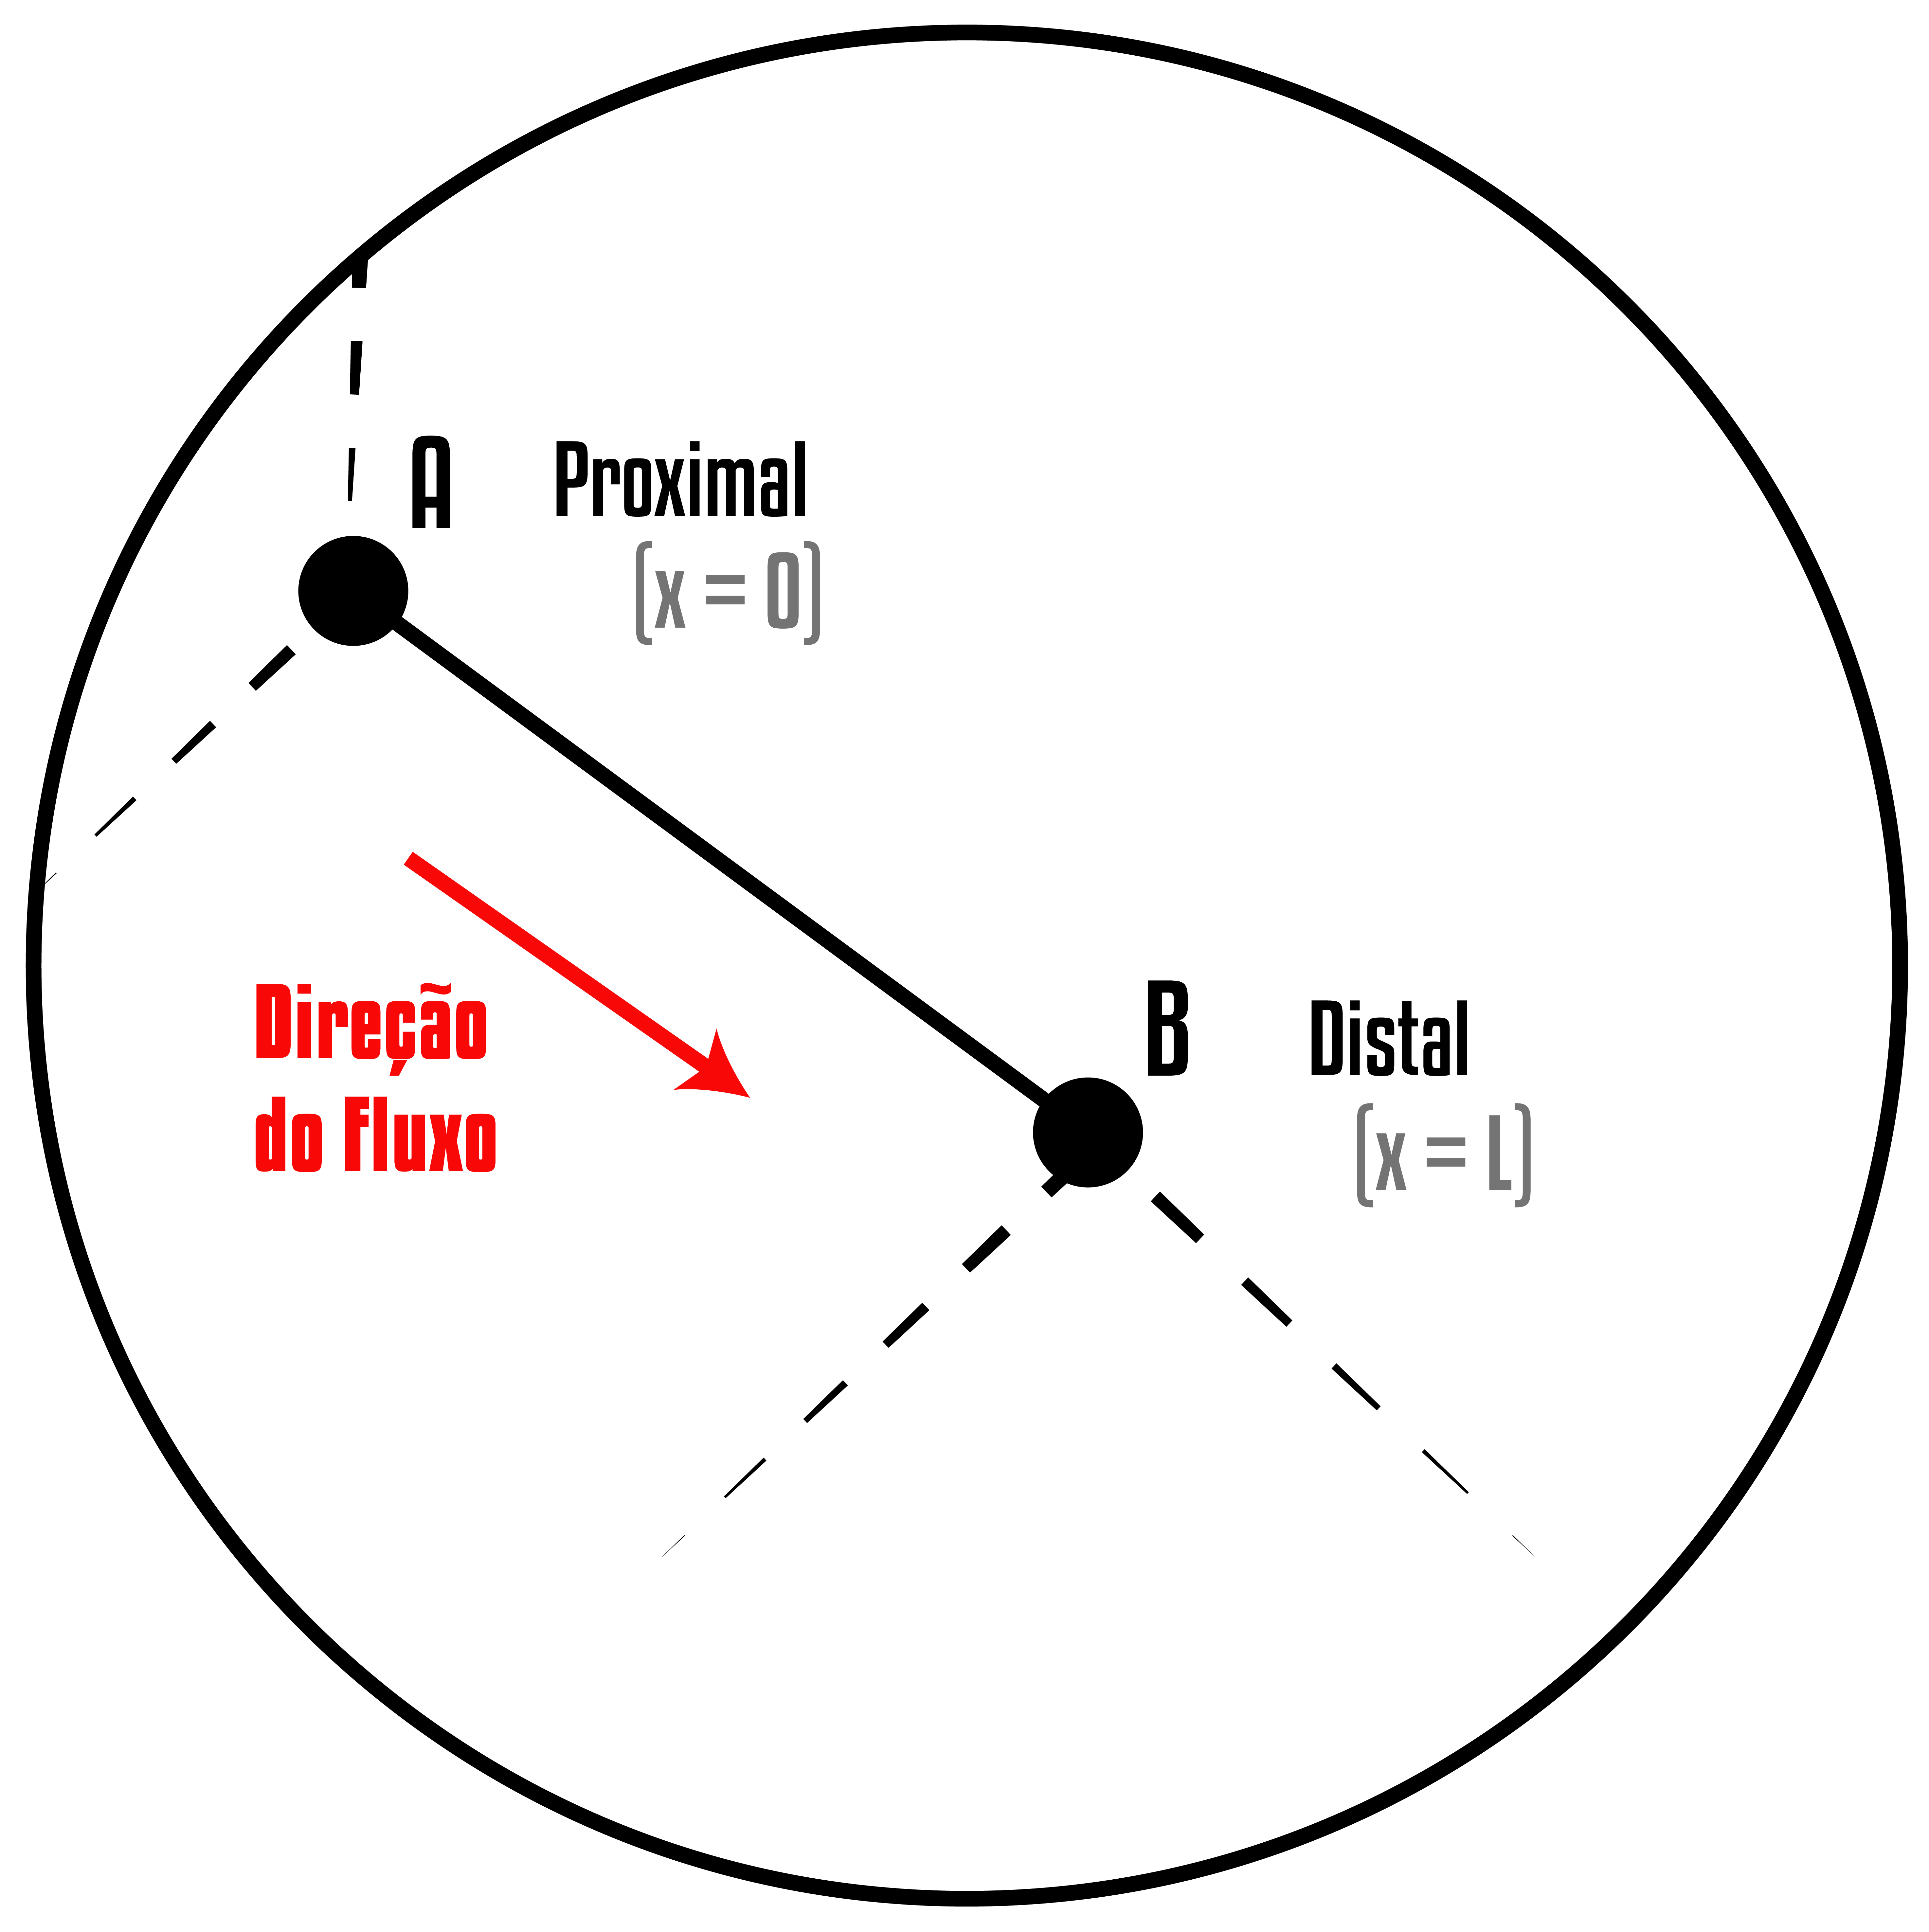
\includegraphics[scale=1]{Figures/ProximalDistal@16x.png}
	\caption{Segmento do modelo geométrico de uma árvore arterial, composto pelo nó proximal $A$ e pelo nó distal $B$.}
	\label{fig:proximaldistal}
\end{figure}

As Equações \eqref{03_p} e \eqref{04_1} para pressão e fluxo são aplicadas em cada segmento de vaso do modelo de árvore arterial, tomando $x = 0$ para o nó proximal e $x = L$ para o nó distal do segmento. Um segmento de vaso é definido pelo intervalo vascular entre dois locais de ramificação \cite{Zamir3}. No sistema arterial, as bifurcações são os locais de ramificação mais comuns~\cite{Zamir1}.

De~\citeyear{Duan}~\citeauthoronline{Duan}, um segmento de vaso é identificado por $(k,j)$, onde o $k$ representa o nível da geração e $j$ representa a ordem do segmento naquela geração, como na Figura~\ref{fig1:arterial-tree}. Desta forma, a pressão e o fluxo ao longo de um segmento  $(k,j)$ do modelo de árvore arterial são dados por:
\begin{eqnarray}
	p(k,j) &=& \bar{p}(k,j) \exp\left[i\omega\left(t - \frac{x(k,j)}{c(k,j)}\right)\right] \nonumber \\
	&+& R(k,j)  \bar{p}(k,j) \exp\left[i\omega\left(t - \frac{2L(k,j)}{c(k,j)} + \frac{x(k,j)}{c(k,j)}\right)\right],
	\label{05_p}\\
	q (k,j) &=& Y(k,j)\left\{\bar{p}(k,j) \exp\left[i\omega\left(t - \frac{x(k,j)}{c(k,j)}\right)\right]\right. \nonumber \\
	&-& \left. R(k,j)  \bar{p}(k,j) \exp\left[i\omega\left(t - \frac{2L(k,j)}{c(k,j)} + \frac{x(k,j)}{c(k,j)}\right)\right]\right\},
	\label{06_q}
\end{eqnarray}
nos quais $\bar{p}(k,j)$ é a amplitude combinada do grupo de ondas progressivas no segmento $(k,j)$ e $R(k,j)$ é o coeficiente de reflexão no final daquele segmento. \igunew{O coeficiente de reflexão $R$ é a razão das ondas progressivas pelas ondas atrasadas avaliadas no nó distal $x(k,j) = L(k,j)$. }

O grupo de ondas progressivas viaja no sentido positivo de $x(k,j)$, estas são compostas de ondas progressivas vindo de vasos acima deste, bem como, ondas refletidas na junção à montante $x(k,j) = 0$. O grupo de ondas atrasadas viaja no sentido oposto e é composto por ondas vindas de vasos conectados ao nó distal, estas ondas são refletidas na junção à jusante $x(k,j) = L(k,j)$\igunew{, estas ondas viajam na direção oposta ao fluxo sanguíneo e são consideradas a reflexão  das ondas progressivas nos segmentos adjacentes ao nó distal $B$}. 

As Equações \eqref{05_p} e \eqref{06_q} descrevem, respectivamente, as ondas de pressão e de fluxo localmente em um segmento $(k,j)$ do modelo de árvore, e localmente na posição $x(k,j)$ dentro deste segmento de vaso. \igunew{O principal objetivo deste modelo matemático é determinar as duas variáveis desconhecidas: a amplitude da pressão  $\bar{p} (k,j)$} e o coeficiente de reflexão $R (k,j)$, que são detalhados na Seção~\ref{sec:pressao-fluxo}. 

A Figura~\ref{fig1:arterial-tree} mostra a notação usada para identificar cada segmento de vaso $(k,j)$, onde $k$ é a geração/nível do vaso e $j$ é um número sequencial dentro daquela geração. Os nós proximal e distal do segmento $(k,j)$ são denotados por $A$ e $B$ na Figura~\ref{fig:proximaldistal}, respectivamente. O coeficiente de reflexão $R(k,j)$ do segmento $(k,j)$ está associado ao nó distal $B$.

Na Equação~\eqref{06_q}, tem-se a admitância característica para cada segmento dada por:
\begin{equation}
	Y(k,j) = \frac{A(k,j)}{\rho(k,j)c(k,j)},
	\label{eq:admitancia}
\end{equation}
nos quais $A(k,j)$ é a área da seção transversal do segmento $(k,j)$, $\rho(k,j)$ é a densidade do fluido dentro do vaso e $c(k,j)$ é a velocidade da onda correspondente. A admitância de um segmento é uma medida do quanto o segmento permite o fluxo.

Assumindo um segmento elástico de parede fina, a velocidade da onda $c(k,j)$ é calculada
por~\cite{Fung}:
\begin{equation}
	c(k,j) = \sqrt{\frac{E(k,j) h(k,j)}{\rho(k,j) d(k,j)}},\label{eq:velocidade}
\end{equation}
onde $E(k,j)$ é o módulo de Young, $d(k,j)$ é o diâmetro do segmento $(k,j)$ e $h(k,j)$ é a espessura da parede do segmento, a qual neste estudo é dada por~\cite{Duan}: 
\begin{equation}
	h(k,j) = 0,05 d(k,j).
\end{equation}

\begin{figure}[h] 
	\begin{center}
		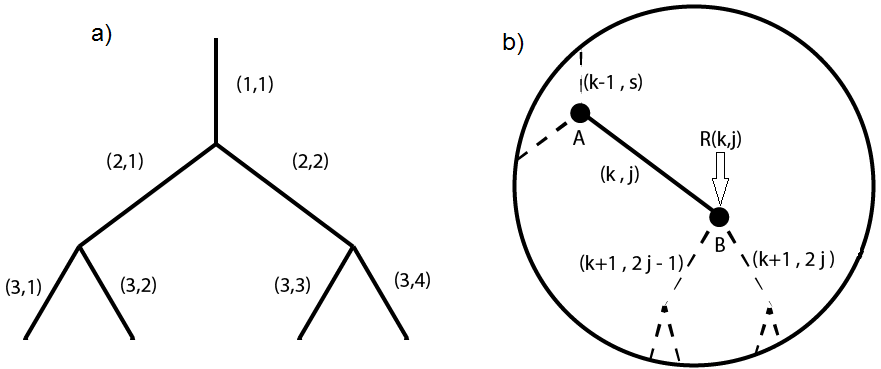
\includegraphics[scale = 0.5]{Figures/ArterialTree_Zamir.png}%
		\caption{Notação usada para identificar cada segmento de vaso $(k,j)$ (figura adaptada de~\citeauthoronline{Duan}(\citeyear{Duan})). }
		\label{fig1:arterial-tree}%
	\end{center}
\end{figure}

%--------------------------------------------------------------------------------%
\subsection{CÁLCULO DA PRESSÃO E DO FLUXO SANGUÍNEO}\label{sec:pressao-fluxo}

Para determinar a pressão $\bar{p} (k,j)$ em um certo segmento $(k,j)$, aplica-se a condição de continuidade de pressão no nó proximal $A$ (ver Figura \ref{fig1:arterial-tree}). Escrevendo as componentes progressiva e atrasada da onda como $p_f (k,j)$ e $p_b (k,j)$ respectivamente, a pressão na posição proximal do segmento  $x(k,j) = 0$ é dada por:
\begin{equation}
	\left[ p (k,j) \right]_A = \left[ p_f (k,j) \right]_A + \left[ p_b (k,j)\right]_A,
	\label{09_p}
\end{equation}
nos quais as pressões $\left[ p_f(k,j) \right]_A$ e $\left[ p_b(k,j) \right]_A$ são expressas por:
\begin{eqnarray}
	\left[ p_f(k,j) \right]_A &=& \bar{p}(k,j)\exp\left[ i\omega t\right],
	\label{10_p_f}\\
	\left[ p_b (k,j) \right]_A &=& R(k,j)\bar{p}(k,j)\exp\left[i\omega \left(t - \frac{2L(k,j)}{c(k,j)}\right) \right].
	\label{11_p_b}
\end{eqnarray}
Similarmente, a pressão no segmento pai $(k-1,s)$ pode ser escrita como:
\begin{equation}
	p(k-1,s) =  p_f(k-1,s) + p_b (k-1,s),
	\label{12_p|_f}
\end{equation}
nos quais $s$ é um número sequencial do segmento pai e as pressões $ p_f (k-1,s)$ e $p_b (k-1,s)$ são dadas por:
\begin{eqnarray}
	p_f (k-1,s) &=& \bar{p}(k-1,s)\exp\left[i\omega \left(t - \frac{x(k-1,s)}{c (k-1,s)}\right) \right],\\
	\label{13_p_f}
	p_b (k-1,s) &=& R (k-1,s)\bar{p}(k-1,s)\exp\left[ i\omega \left( t - \frac{2L(k-1,s)}{c(k-1,s)} + \frac{x(k-1,s)}{c(k-1,s)}\right) \right]. \nonumber
\end{eqnarray}

No nó distal do vaso superior, $x(k-1,s) = L(k-1,s)$, a pressão é dada por:
\begin{equation}
	\left[ p(k-1,s) \right]_A = \left[ p_f(k-1,s)\right]_A + \left[ p_b(k-1,s) \right]_A,
	\label{13_p|_f}
\end{equation}
nos quais 
\begin{eqnarray}
	\left[ p_f(k-1,s) \right]_A &=& \bar{p}(k-1,s)\exp\left[ i\omega \left(t - \frac{L(k-1,s)}{c(k-1,s)}\right)\right],
	\label{15_p_f}
	\\
	\left[ p_b(k-1,s) \right]_A &=& R(k-1,s)\bar{p}(k-1,s)\exp\left[i\omega \left( t - \frac{L(k-1,s)}{c(k-1,s)} \right) \right]. 
	\label{16_p_b}
\end{eqnarray}

A condição de continuidade da pressão exige que na junção ela assuma um único valor, portanto
\begin{equation}
	\left[ p_f(k-1,s) \right]_A + \left[ p_b (k-1,s) \right]_A = \left[ p_f(k,j) \right]_A + \left[ p_b(k,j) \right]_A.
	\label{17_p_cont}
\end{equation}

Substituindo as Equações \eqref{10_p_f}, \eqref{11_p_b}, \eqref{15_p_f} e \eqref{16_p_b} na Equação \eqref{17_p_cont} e resolvendo para $\bar{p}(k,j)$, resulta em:
\begin{equation}
	\bar{p} (k,s) =  \frac{\bar{p}(k-1,s)\left[1 + R(k-1,s)\right] \exp\left[ -\frac{i \omega L(k-1,s)}{c(k-1,s)}\right]}{1 + R(k,j)\exp{\left[ -2i\omega \frac{L(k,j)}{c(k,j)}\right]}}.
	\label{18_barp}
\end{equation}

Conforme~\citeauthoronline{Duan}(\citeyear{Duan}), para efeitos de cálculo da pressão e fluxo, adimensionalizam-se as pressões em \eqref{18_barp} em termos da pressão de entrada $p_0 = \bar{p}_0 \exp[i\omega t]$. 

Considerando $P(k,j) = \frac{p(k,j)}{p_0}$ e $\bar{P} (k,j) = \frac{\bar{p}(k,j)}{\bar{p}_0}$, a Equação~\eqref{05_p} para o cálculo da pressão  pode ser expressa de forma adimensionalizada por:
\begin{eqnarray}
	P(k,j) &=& \bar{P}(k,j)\big\{\exp[ -i\beta(k,j) X(k,j)] \nonumber \\
	& +& R(k,j) \exp[-i2\beta(k,j)] \exp[i\beta(k,j) X(k,j)]\big\},
	\label{21_P}
\end{eqnarray}
nos quais $\beta(k,j) = \frac{\omega L(k,j)}{c(k,j)}$ e $X = \frac{x(k,j)}{L(k,j)}$. Similarmente, a Equação~\eqref{06_q} para o fluxo $q(k,j)$ pode ser obtida de forma adimensionalizada por:
\begin{eqnarray}
	Q(k,j) &=& M(k,j)\bar{P}(k,j)\big\{ \exp\left[ -i\beta(k,j) X(k,j) \right] \nonumber \\ 
	&-& R(k,j) \exp[ -2i\beta(k,j)] \exp[i\beta(k,j) X(k,j)] \big\},
	\label{23_Q}
\end{eqnarray}
nos quais $Q(k,j) = \frac{q (k,j)}{q_0}$, $M = \frac{Y(k,j)}{Y(1,1)}$ e $q_0 = Y(1,1)p_0$. O cálculo da admitância $Y(1,1)$ na posição proximal do segmento raiz, ou seja, da artéria de alimentação é apresentado na próxima seção.

%------------------------------------------------------------%
\subsection{CÁLCULO DO COEFICIENTES DE REFLEXÃO E ADMITÂNCIA}

Para determinar os coeficientes de reflexão nas junções, consideram-se as duas junções $A$ e $B$ das extremidades de um segmento genérico $(k,j)$ de um modelo de árvore arterial (ver Figura~\ref{fig1:arterial-tree}). Na posição distal $B$, o coeficiente de reflexão é definido por~\cite{Fung,Lighthill}:
\begin{equation}
	R(k,j) = \frac{Y(k,j) - [Y_e(k+1,2j) + Y_e(k+1,2j-1)]}{Y(k,j) + [Y_e(k+1,2j) + Y_e(k+1,2j-1)]},
	\label{27_R}
\end{equation}
nos quais $Y_e(k+1,2j-1)$ e $Y_e(k+1,2j)$ são admitâncias efetivas nos segmentos à jusante de $B$. Estas admitâncias são determinadas pela razão entre o fluxo e pressão naquela posição, que é dada por:
\begin{equation}
	Y_e(k+1,s) = \frac{Y(k+1,s)\left\{1 - R(k+1,s)\exp{[-i2\beta(k+1,s)]}\right\}}{1 + R(k+1,s)\exp{[-i2\beta(k+1,s)]}},
	\label{28_Ye}
\end{equation}
nos quais $s = 2j-1$ e $2j$ são os números sequenciais dos dois segmentos filhos e $R(k+1,s)$ é o coeficiente de reflexão na posição distal de cada segmento. Similarmente, $Y_e(k,j)$, a admitância na posição proximal $A$ do segmento $(k,j)$ pode ser dada por:
\begin{equation}
	Y_e(k,j) = \frac{Y(k,j)\{1 - R(k,j)\exp{[-i2\beta(k,j)]}\} }{1 + R(k,j)\exp{[-i2\beta(k,j)]}}
	\label{29_Ye}.
\end{equation}
Substituindo $R(k,j)$ da Equação \eqref{27_R} em \eqref{29_Ye}, obtém-se  uma equação para cálculo das admitâncias efetivas ao longo do modelo de árvore arterial:
\begin{equation}
	Y_e(k,j) = \frac{Y(k,j) [Y_e(k+1,2j) + Y_e(k+1,2j-1)+ i Y(k,j)\tan{\beta(k,j)}]}{Y(k,j) + i[Y_e(k+1,2j) + Y_e(k+1,2j-1)]\tan{\beta(k,j)}}.
	\label{30_Ye}
\end{equation}

Em segmentos terminais, pode ser assumido que não ocorrem mais reflexões à jusante das posições distais destes segmentos, portanto a admitância efetiva destes segmentos é igual às suas admitâncias características. Adotando a Equação \eqref{29_Ye}, todas as admitâncias efetivas podem ser determinadas percorrendo a árvore a partir dos segmentos terminais até o segmento raiz.

\subsection{CÁLCULO DA IMPEDÂNCIA DE ENTRADA}

A impedância vascular de um modelo de árvore arterial é expresso por
\begin{equation}
	z = \frac{p}{q},
\end{equation}
onde $p$ e $q$ podem ser definidos pelas Equações \eqref{03_p} e \eqref{04_1}, respectivamente. Dados que $p(k,j) = P(k,j) p_0$, $q(k,j) = Q(k,j) q_0$ e $q_0 = Y(1,1) p_0$, em termos de variáveis adimensionalizadas, a impedância pode ser reescrita por
\begin{equation}
	Z = \frac{P(k,j)}{Y(1,1) Q(k,j)}.
\end{equation}

A impedância de entrada de um modelo de árvore arterial determina $Z$ na posição proximal do vaso raiz, ou seja, em $x (k,j) = 0$. 

Adotando as Equações~\eqref{21_P} e~\eqref{23_Q} com $x (k,j) = 0$, obtém-se a impedância de entrada:
\begin{equation}
	Z = \frac{-1}{Y(1,1)}.
\end{equation}
Em suma, a impedância de entrada  em módulo é o inverso da admitância característica da artéria de alimentação.

%--------------------------------------------------------------------------------%
\subsection{INCORPORAÇÃO DA VISCOSIDADE E VISCOELASTICIDADE NO MODELO}
\label{sec:cenario}
A partir do modelo matemático aqui apresentado, os seguintes cenários podem ser investigados nas simulações hemodinâmicas:
\begin{itemize}
	\item \textbf{2.1.4.1 - Cenário 1}: análise do impacto da viscosidade sanguínea ($\mu(k,j)$).\\
	Os efeitos da viscosidade sanguínea podem ser investigados por substituir a velocidade
	da onda $c(k,j)$ por uma velocidade da onda complexa:
	\begin{equation} 
		c_v(k,j) = c(k,j) \sqrt{\epsilon},\label{eq:velocidade-complexa}
	\end{equation}
	onde $\epsilon$ é um fator viscoso que corresponde a um tubo elástico com restrições~\cite{Duan1992}. Seja $\alpha$ o
	número de Womersley adimensional
	\begin{equation}
		\alpha = r(k,j) \sqrt{\frac{\omega \rho(k,j)}{\mu(k,j)}},
	\end{equation}
	o fator viscoso $\epsilon$ é calculado por:
	\begin{equation}
		\epsilon = 1 - F_{10} (\alpha),
	\end{equation}
	onde a função $F_{10}$ é avaliada deste modo:
	\begin{equation}
		F_{10} (\alpha) = \frac{2}{\alpha \sqrt{i}}(1+\frac{1}{2\alpha}),
	\end{equation}
	onde $J_p$ denota a função de Bessel de índice $p$.
	
	\item \textbf{2.1.4.2 - Cenário 2}: análise do impacto da viscoelasticidade da parede do vaso ($\phi_0$).\\
	A viscoelasticidade da parede do segmento é incorporada substituindo o módulo de Young
	estático $E(k,j)$ por um módulo elástico complexo $E_c(k,j)$ no cálculo da velocidade $c(k,j)$ na equação~\eqref{eq:velocidade}
	da seguinte forma~\cite{Duan}:
	\begin{equation}
		E_c(k,j) = |E_c(k,j)| \exp\{i\phi\},\label{eq:Young}
	\end{equation}
	onde $\phi$ é o ângulo de fase entre a pressão e o deslocamento da parede do segmento \cite{Taylor3} expresso por $\phi = \phi_0 [1-\exp(-\omega)]$ e $|E_c (k,j)|$ corresponde ao módulo de Young fornecido para a simulação.
	
	\item \textbf{2.1.4.3 - Cenário 3}: efeitos da viscosidade sanguínea $\mu(k,j)$ e da viscoelasticidade da parede do segmento $\phi_0$ de forma combinada.
	
	Neste último cenário, utiliza-se a Equação~\eqref{eq:Young} para determinar a velocidade da onda $c(k,j)$~\eqref{eq:velocidade} no modelo. Com este resultado, calcula-se  a Equação~\eqref{eq:velocidade-complexa} para determinar a velocidade complexa $c_v(k,j)$ a ser considerada no modelo.
\end{itemize}





%--------------------------------------------------------------------------------%
%\chapter{FERRAMENTA COMPUTACIONAL}\label{sec:ferramenta_computacional}

Nesta seção apresentam-se detalhes da ferramenta computacional desenvolvida para simulação do escoamento sanguíneo em modelos de árvores arteriais. A principal finalidade desta ferramenta é possibilitar a visualização de estruturas das árvores arteriais e após a simulação hemodinâmica,  a visualização das curvas de distribuição do fluxo sanguíneo e pressão.

Esta ferramenta foi desenvolvida em C++ utilizando as bibliotecas comuns do Qt 5.15.0 \cite{QTClasses} e OpenGL \cite{OpenGL}, que ajudam na construção da interface gráfica e na exibição de modelos gráficos, como árvores arteriais e gráficos. A ferramenta foi disponibilizada em dois ambientes, o primeiro nomeado de \textit{Iterador Gráfico Universal} (IGU), pois em seu modelo de classes qualquer objeto que implemente a classe \textit{WiseObject}, elucidada na Seção~\ref{sec:estrutura}, está apto para realizar iterações e desenhar-se através de diretivas OpenGL em um elemento de interface gráfica. O segundo ambiente disponibilizado foi nomeado de \textit{Iterador não-Gráfico Universal} (InGU), pois segue a mesma generalização, entretanto é disponibilizada pelo console, não possuindo interface gráfica. Buscou-se no desenvolvimento desta ferramenta alto grau de generalização para que seja possível analisar todos os parâmetros de um objeto facilmente e que ela possua grande versatilidade. Além de árvores arteriais a ferramenta possibilita que outros objetos sejam geradas para visualização.

A Figura~\ref{fig1:gui} ilustra a ferramenta desenvolvida. À seguir, apresentam-se em detalhes a implementação computacional realizada.

\begin{figure}[!htbp]
	\centering
	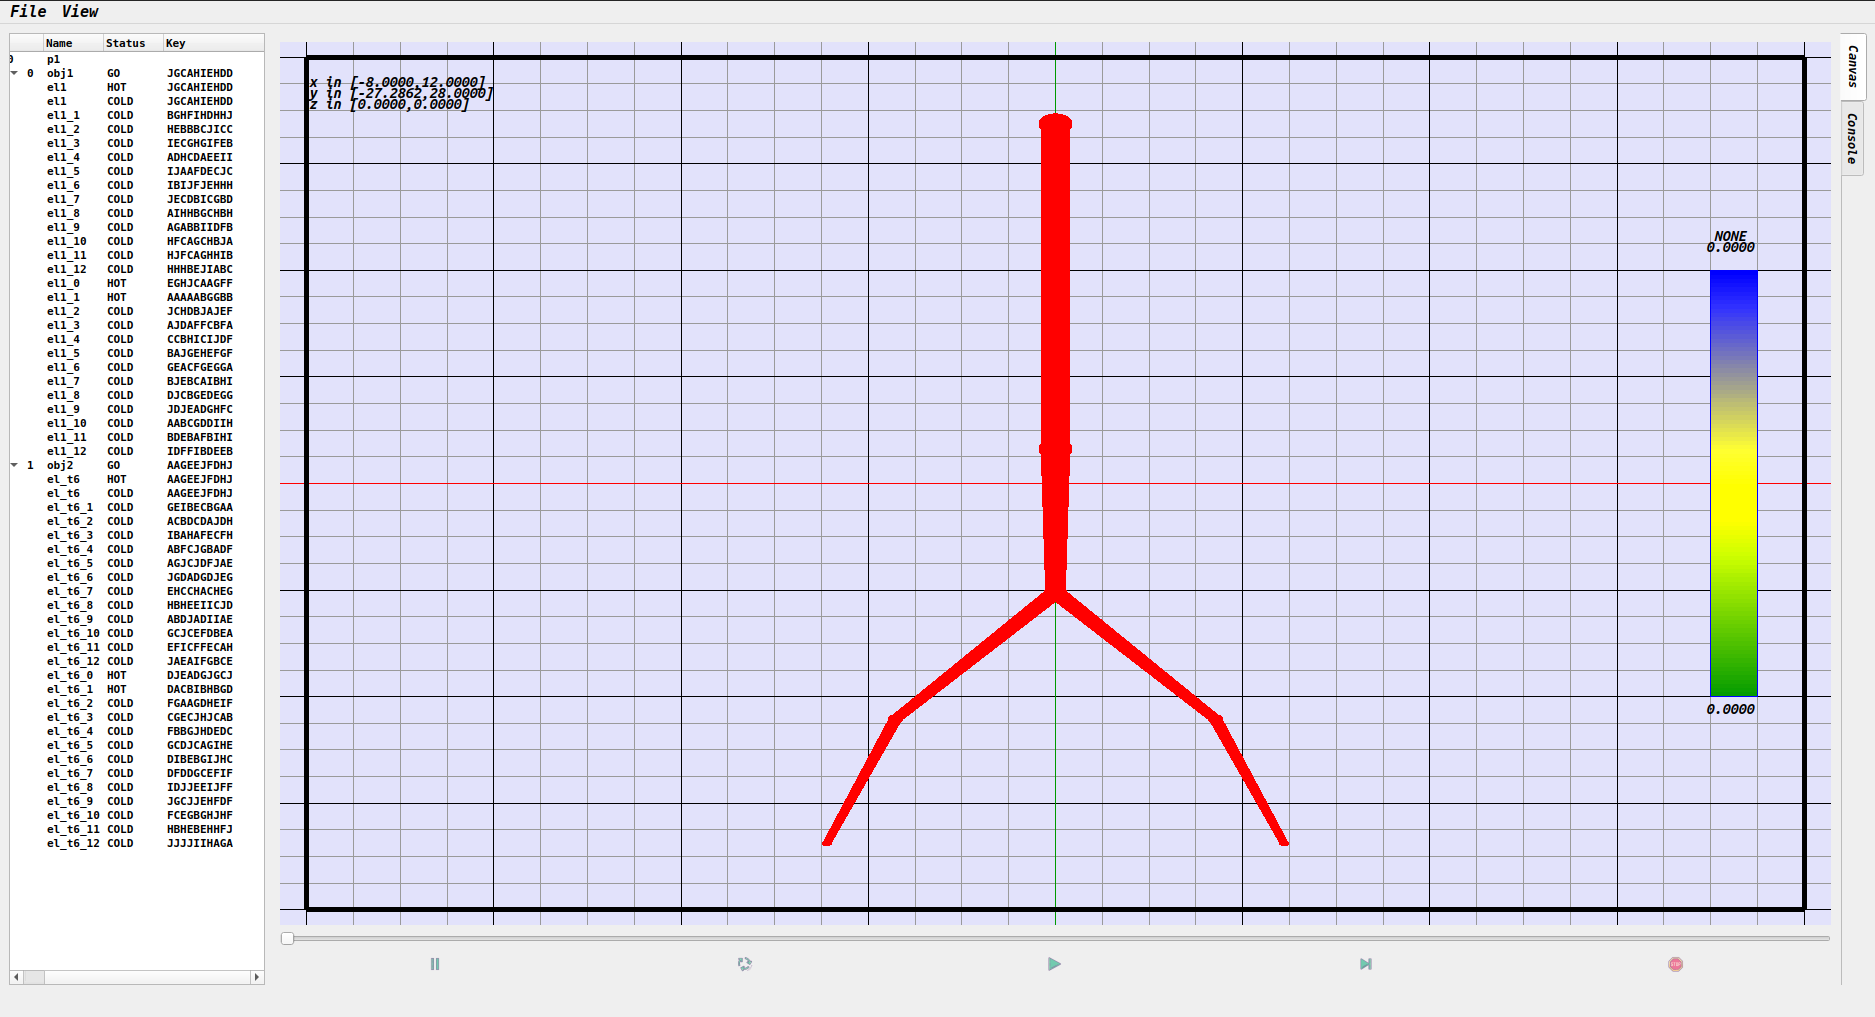
\includegraphics[scale=0.25]{Figures/IGU_002.png}
	\caption{Interface gráfica da ferramenta desenvolvida.}
	\label{fig1:gui}
\end{figure}

Através da modelagem de classes no paradigma do C++ \cite{AlanParker}, foi possível realizar diversas generalizações que ampliam a adaptabilidade dos objetos que podem ser inseridos neste modelo de classes. Na seção seguinte apresentamos um esquema de classes virtuais, ou abstratas, que foram criadas para facilitar o manuseio dos objetos dentro do ambiente computacional e prover funções básicas. 

Uma classe virtual não possui construtor próprio, porque classes virtuais são incompletas. Estas classes possuem métodos virtuais, que por sua vez precisam ser definidos pela classe herdeira. Portanto uma classe virtual funciona como um conjunto de regras que classes herdeiras devem seguir, todas as classes que implementem esta classe virtual devem ter sua própria definição dos métodos virtuais, podendo ter funcionamentos distintos, entretanto recebendo os mesmo parâmetros.  Adicionado este conceito à estrutura de dados, classes virtuais generalizam os objetos e garantem o seu funcionamento, separando as estruturas de acordo com seu propósito em classes.

%--------------------------------------------------------------------------------%
\section{ESTRUTURA DE DADOS}\label{sec:estrutura}

Nesta seção apresentam-se detalhes da estrutura de dados adotada no funcionamento da ferramenta computacional. Como mencionado na Seção~\ref{sec:algoritmo}, uma estrutura de ponteiros é utilizada,  sendo capaz de armazenar todas as informações do modelo geométrico da árvore arterial. A ferramenta computacional foi desenvolvida para ser capaz de armazenar, carregar e iterar o modelo matemático e gerar novas estruturas para visualização, a estrutura de dados proposta para a ferramenta precisa realizar estar operações e armazenar corretamente os dados gerados.

As seções à seguir descrevem a estrutura de dados genérica, tendo como principal objeto de estudo, o fluxo pulsátil enquanto atravessa uma estrutura de árvore arterial e a visualização de seus resultados. Em versões anteriores, a ferramenta computacional definia seus modelo matemáticos, geométricos e de visualização em apenas uma estrutura abstrata, o que acarretou em classes grandes com difícil manutenção e pouca versatilidade. Isto porque o mesmo objeto ficava responsável por diversas funções, era capaz de se instanciar, iterar e desenhar na tela através de diretivas OpenGL. Portanto, nesta versão da ferramenta computacional as classes foram desenvolvidas para ter propósito único, cujo objetivo é garantir que as classe tenham uma função apenas, garantindo uma classe enxuta e de fácil interpretação.

Com a experiência adquirida previamente três principais fluxos foram identificadas:  A iteração dos objetos, uma vez carregados estes objetos são atualizados por algoritmos, gerando novas versões; O armazenamento dos objetos, os elementos criados no método de iteração podem ser armazenados em um cache e então recuperados;  E a exibição dos objetos, uma vez carregados os objetos podem ser exibidos na tela e visualizados. Entendendo o método iterativo como uma animação em que todos os quadros precisam ser armazenados, o objeto inteligente \textit{WiseObject} foi criado representando toda a animação e o elemento inteligente \textit{WiseElement} como cada quadro da animação. Cada quadro antes de ser exibido precisa ser processado em diretivas OpenGL, o responsável sobre esse processo é o elemento gráfico \textit{GraphicObject}. Igualmente quando se tratam de animações e reproduções de vídeo, somente quadros necessários estarão em memória. 

Finalmente, estas estruturas são utilizadas pela ferramenta computacional possibilitando que modelos geométricos sejam carregados, iterados e então exibidos, sem que haja perda dos quadros ou de algum dado. Os elementos principais da estrutura de dados serão descritos nas seções que se seguem.

%--------------------------------------------------------------------------------%
\subsection{ELEMENTO INTELIGENTE}\label{sec:elemento_inteligente}

Elementos inteligentes são objetos que implementam a classe \textit{WiseElement}, o principal objetivo de um elemento inteligente é manter os dados mais recentes de um modelo geométrico e os dados necessários para o método de iteração. No caso do estudo do fluxo pulsátil consideramos que uma iteração seja a execução completa do algoritmo apresentado na Seção~ \ref{sec:algoritmo} em toda a árvore. Portanto cada elemento inteligente possuirá todas as informações do modelo geométrico de uma árvore arterial, seus segmentos e suas propriedades.

Através das malhas estruturadas e desestruturadas presentes na biblioteca \textit{VTK}(\textit{Visua}-\textit{lization ToolKit}) é possível descrever diversas estruturas de dados através de elementos padronizados, como pontos, linhas e células. Utilizando os elementos básicas contidas nestas malhas, variáveis e ferramentas da linguagem a estrutura básica da arquitetura foi criada, presente na Figura~\ref{fig2:wiselement}.

\begin{figure}[!htbp]
	\centering
	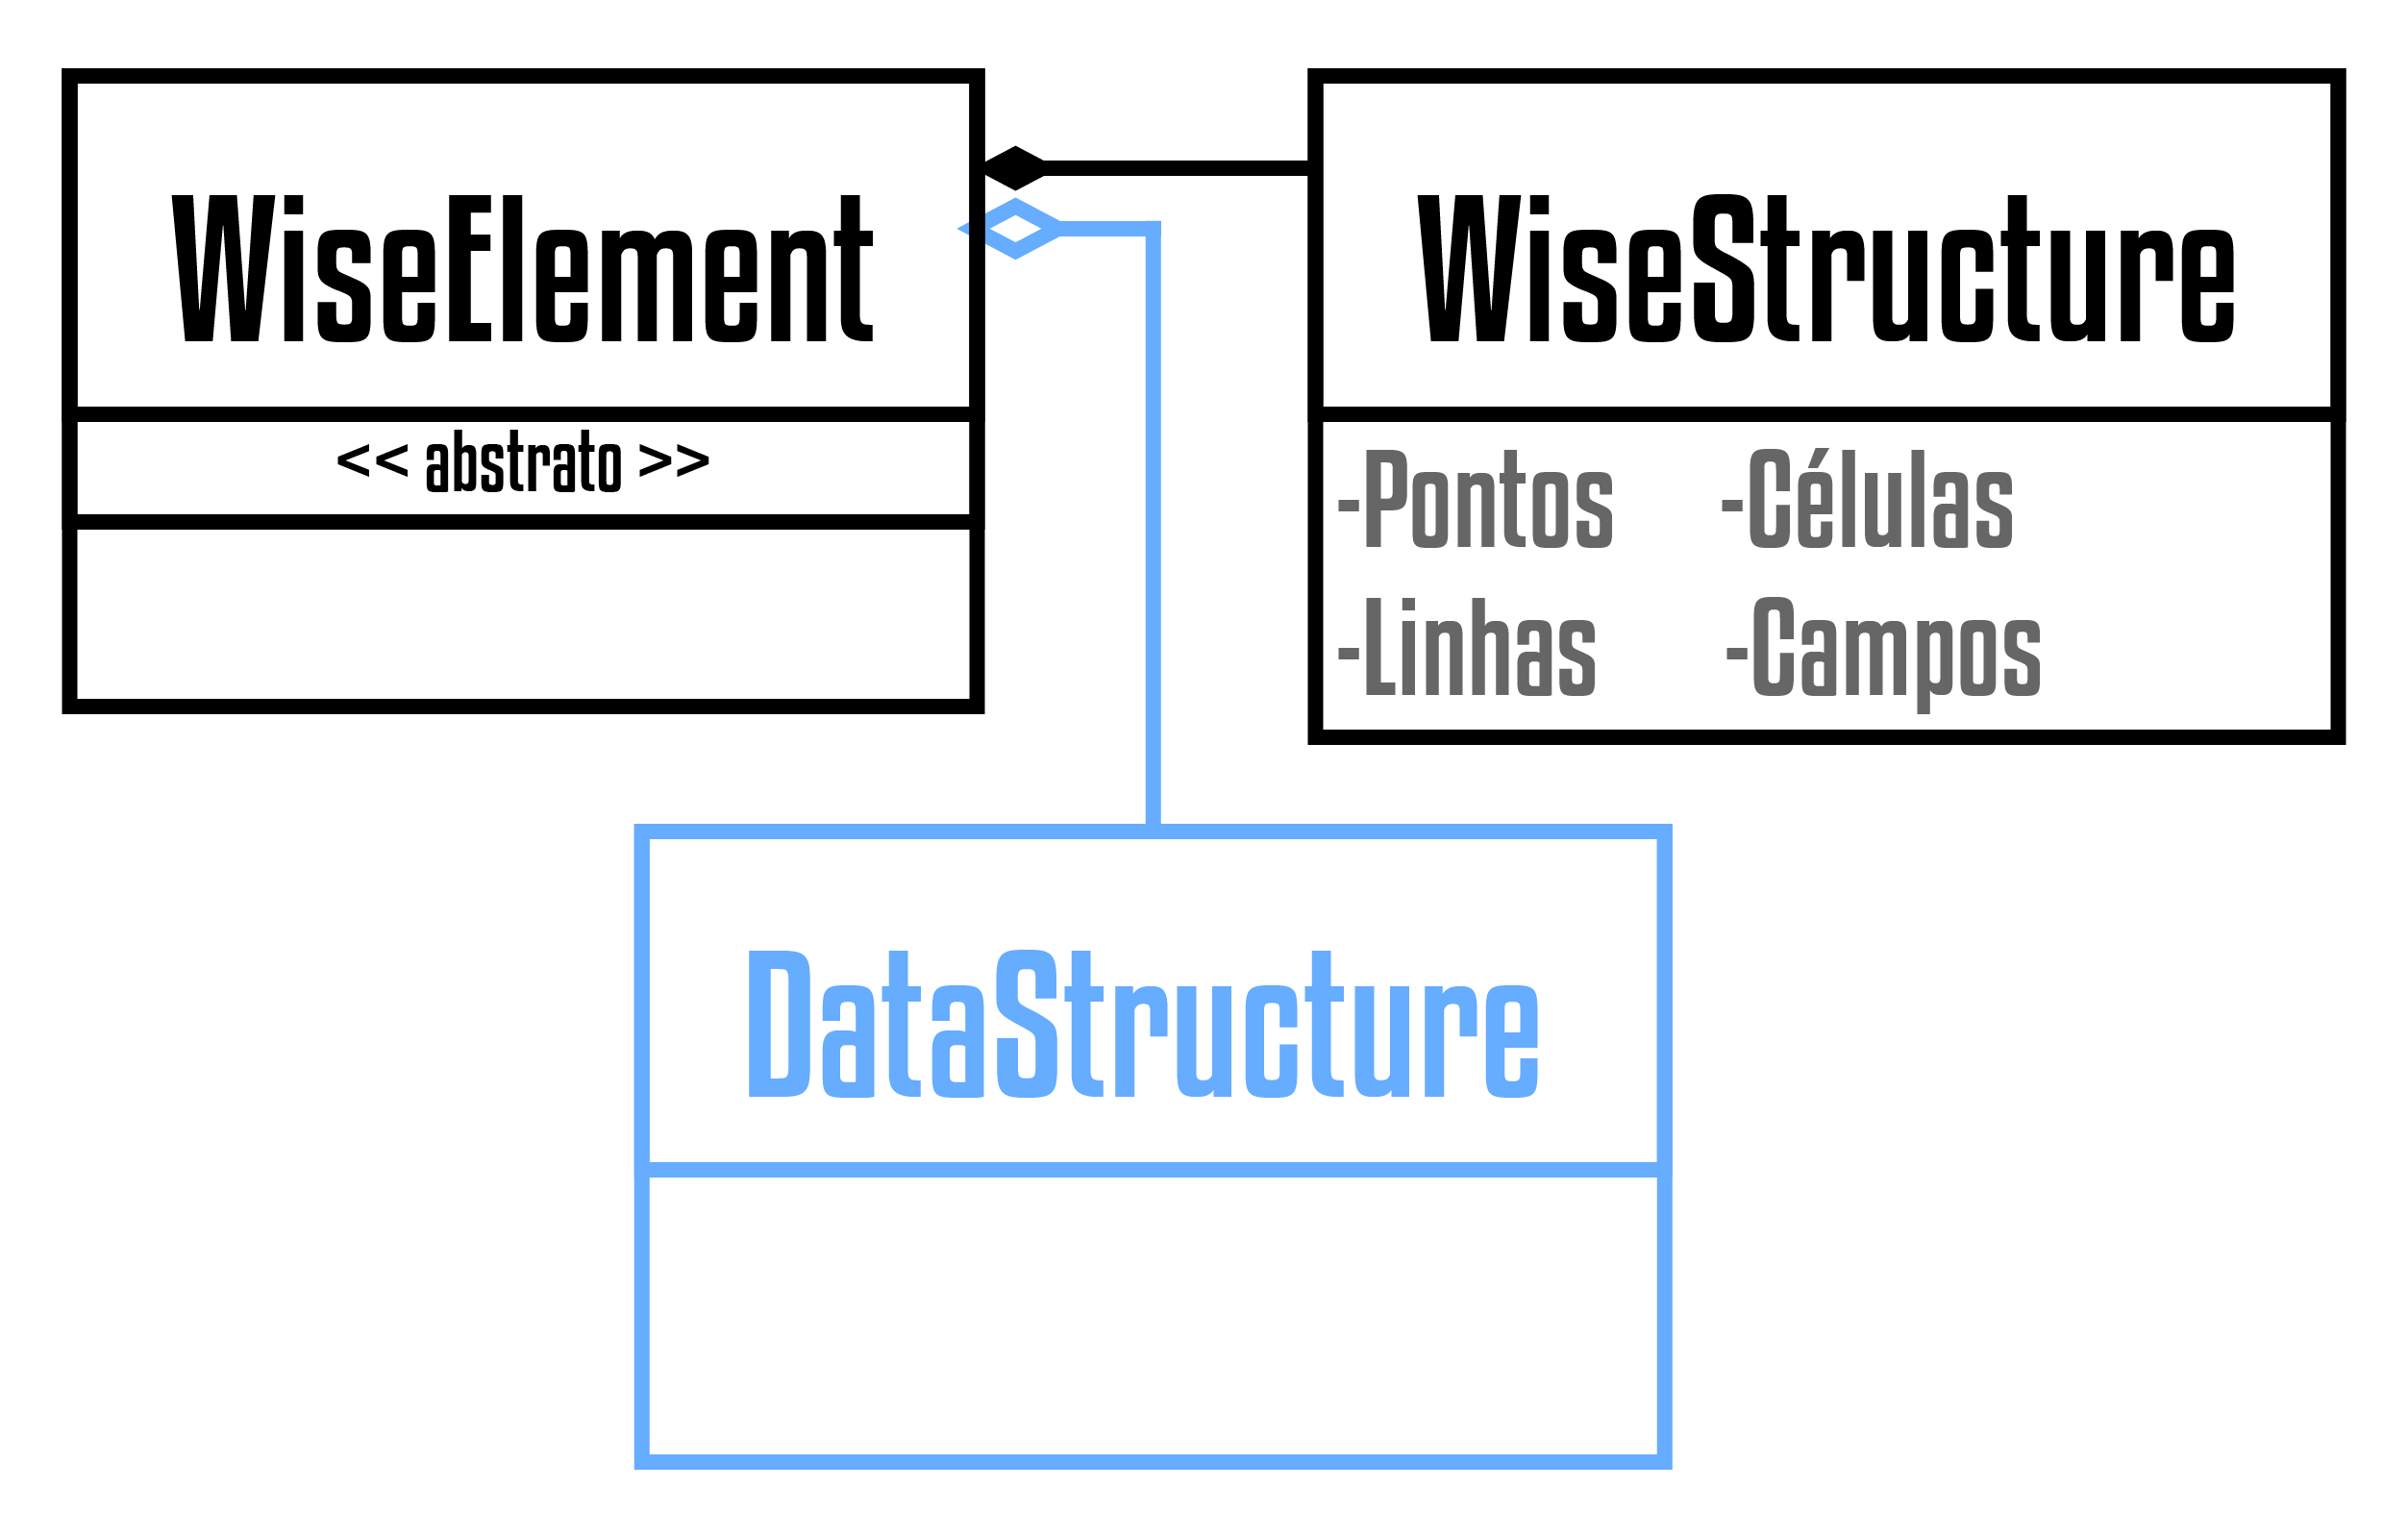
\includegraphics[scale=2]{Figures/WiseElement@16x.png}
	\caption{Representação de classes de um elemento inteligente. WiseElement a classe abstrata base e seus componentes: WiseStructure representa a estrutura contida em um arquivo VTK e DataStructure representa a estrutura de ponteiros e variáveis utilizadas na iteração. Tingido de azul as estruturas que nem sempre estão presentes.}
	\label{fig2:wiselement}
\end{figure}

A Figura~\ref{fig2:wiselement} mostra que um elemento inteligente é composto por duas outras estruturas: A primeira \textit{WiseStructure}, utiliza pontos, linhas, células e campos para determinar estruturas geométricas; A segunda \textit{DataSructure}, representa os dados abstratos específicos de cada elemento. Estas estruturas são equivalentes entre si, isto é feito para que a primeira estrutura siga um formato padrão de pontos, linhas, células e campos seja mantida. Enquanto dados abstratos equivalentes podem ser utilizados. Os dados mantidos na estrutura padrão \textit{WiseStructure} são utilizados principalmente na leitura e escrita de objetos, portanto são mantidos como vetores que possuem cadeias de caracteres, os dados presentes nesta estrutura podem ser editados pelo usuário. Enquanto os dados abstratos contém a mesma informação contida em variáveis da linguagem, como números inteiros, vetores, ponteiros e outros.

Cada parâmetro de um elemento inteligente representa uma grandeza associada à um componente do modelo geométrico (pontos,  linhas e células) ou ainda sobre todo o modelo (campos). Cada parâmetro irá possuir um nome e uma estrutura associada, os raios de um árvore arterial $r$ são dados relacionados às linhas da estrutura e somente um valor será armazenado. Enquanto os valores da onda de uma onda de pressão $P$ através de um segmento com $X \in [0,1]$ estão relacionados as mesmas linhas, mas são representados por uma sequência de valores. Ambos os valores são salvos na mesma estrutura e podem ser acessados da mesma forma.

\begin{figure}[!htbp]
	\centering
	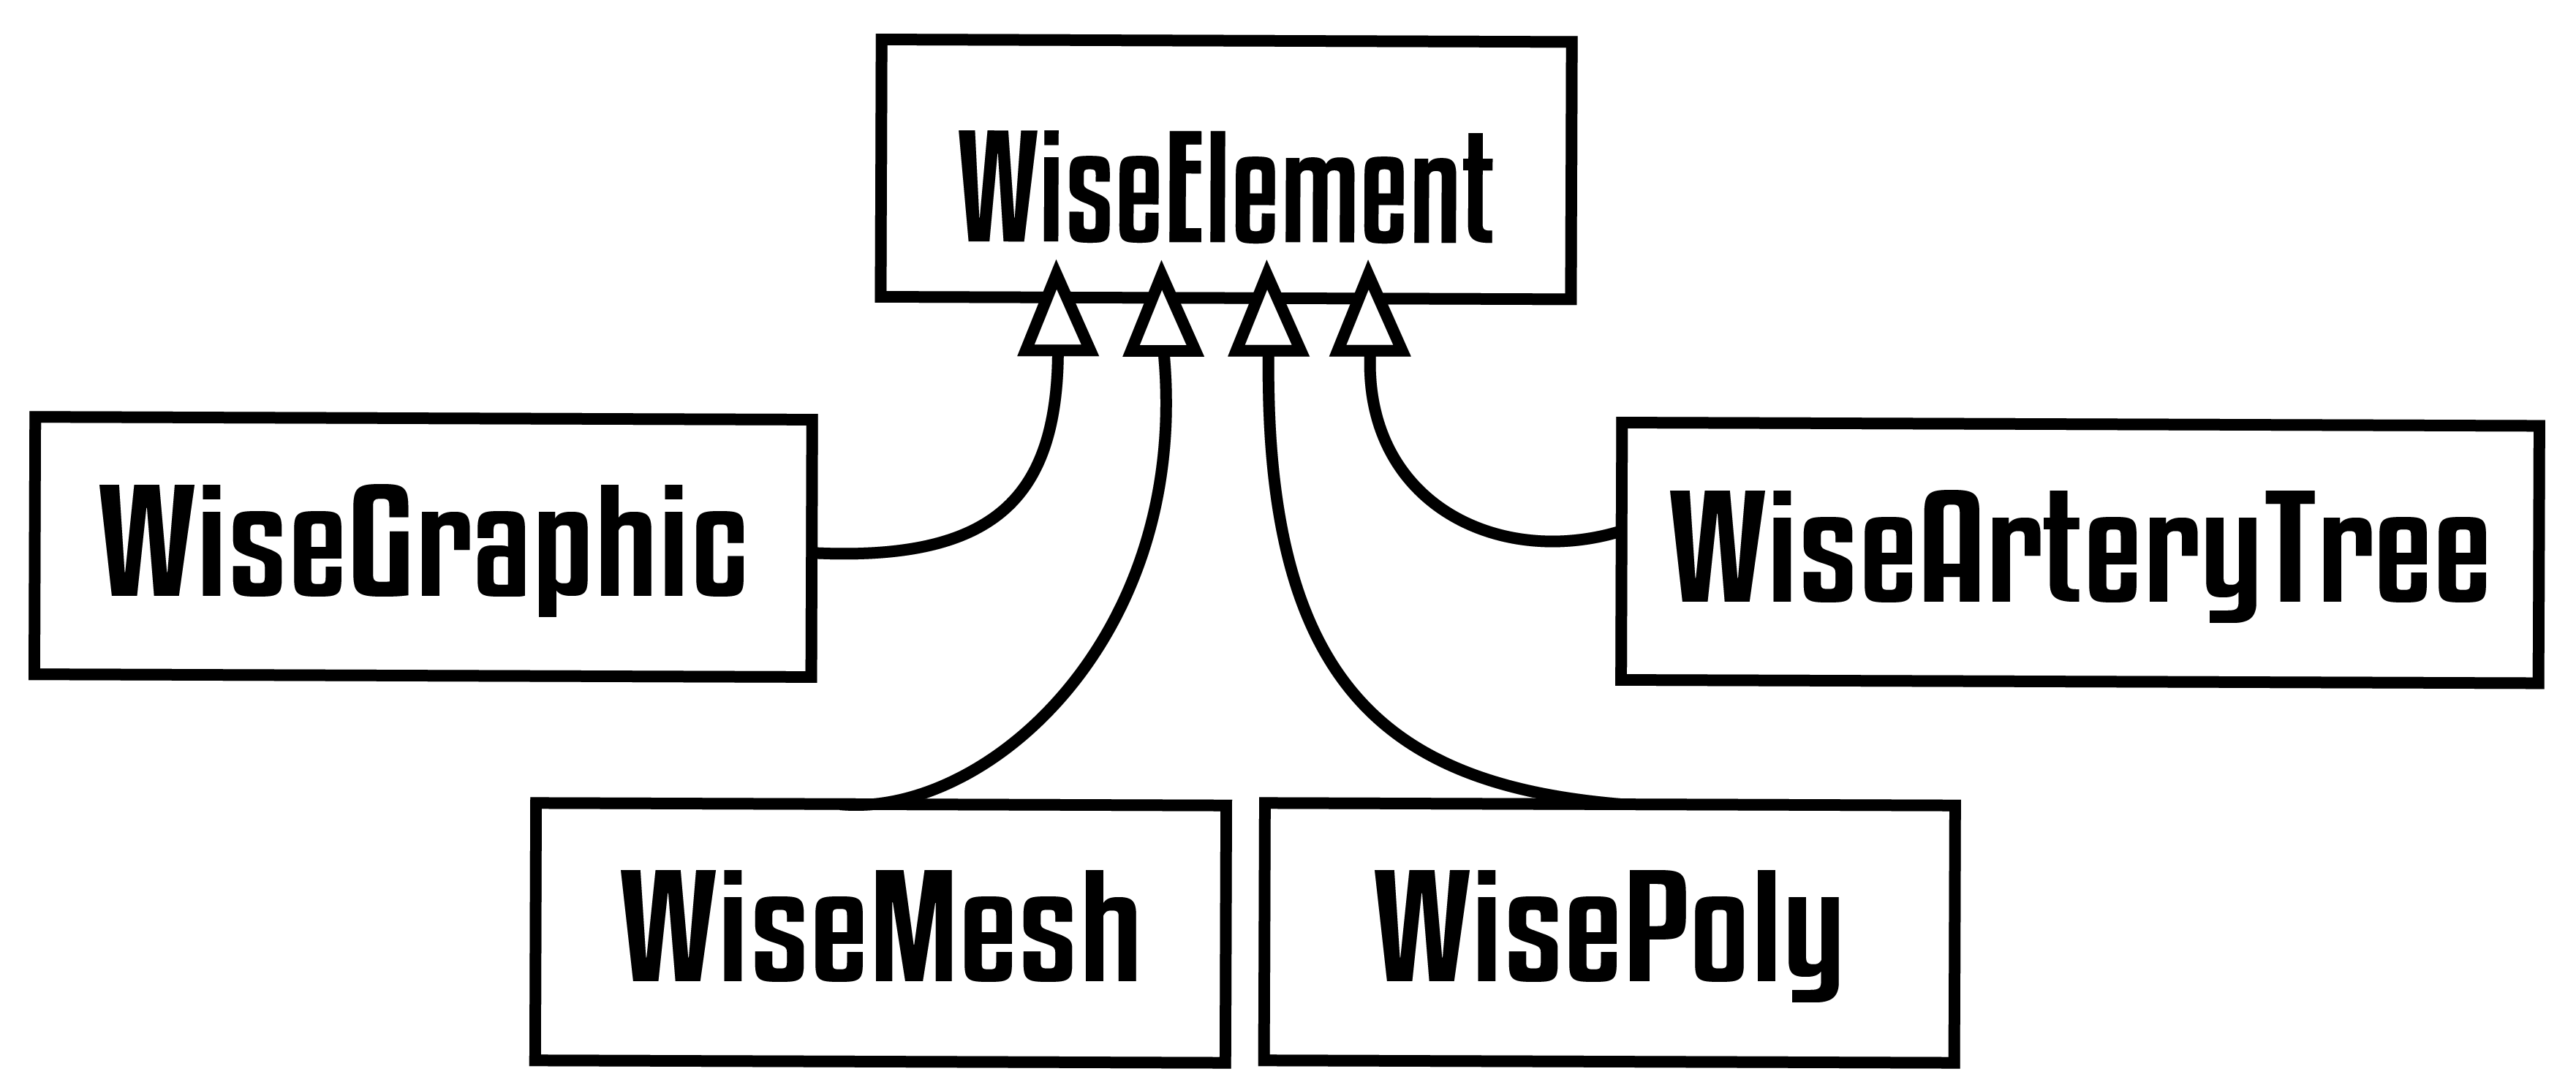
\includegraphics[width=\textwidth]{Figures/WiseElements@16x.png}
	\caption{Tipos de elementos inteligentes. \textit{WiseGraphic}, um gráfico bidimensional. \textit{WiseMesh}, uma malha tridimensional. \textit{WisePoly}, um cubo. \textit{WiseArteryTree}, uma árvore arterial}
	\label{fig2:wiselements}
\end{figure}

Como demonstrado na Figura~\ref{fig2:wiselements} um elemento inteligente é aquele que implementa a classe abstrata \textit{WiseElement}, os dados abstratos \textit{DataStructure} de cada classe podem ser salvos na estrutura padrão \textit{WiseStructure} e utilizados quando necessário. 

O modelo geométrico de uma árvore arterial foi traduzido para o elemento inteligente \textit{WiseArteryTree}, a estrutura inteligente deste elemento conta com pontos e linhas que definem os parâmetros do modelo geométrico na estrutura \textit{WiseStructure}, a estrutura abstrata \textit{DataStructure} conta com ponteiros para cada segmento e grandezas físicas armazenadas em pontos flutuantes de precisão dupla.

O elemento inteligente \textit{WiseGraphic} foi criado para armazenar dados ao longo de uma dimensão, como a pressão ao longo da árvore arterial. Os elementos \textit{WiseMesh} e \textit{WisePoly} foram criados para armazenar dados ao longo de duas dimensões e ao longo de três dimensões, estes dois elementos foram utilizados como exemplo de objetos que podem ser generalizados na ferramenta e visualizados, mudando pouco as estruturas já existentes. O elemento \textit{WiseGraphic} é equivalente à um vetor de valores $(x,v)$, o elemento \textit{WiseMesh} à uma matriz de valores $(x,y,v)$ e o elemento \textit{WisePoly} uma matriz tridimensional de valores $(x,y,z,v)$, onde $v$ é o valor associado e $(x,y,z)$ a posição. Através deste modelo, é possível armazenar em um \textit{WiseMesh} o valor $v$ da pressão ao longo de uma árvore arterial na direção $x$ variando a frequência no eixo $y$.

Os elementos inteligentes servem como estruturas de armazenamento padrão que compõem um outro objeto. O ciclo de manipulação desses elementos se divide em três partes: A criação, aonde os objetos podem ser criados à partir de exemplos pré-definidos ou através de um arquivo de entrada \textit{VTK} ou \textit{XML (eXtensible Markup Language)}; A iteração, processo em que o elemento inteligente com todas as estruturas definidas e consistentes é utilizado por um algoritmo; A exibição, este último ciclo utiliza a estrutura atualizada e gera um objeto para visualização.

Todo elemento inteligente completo possui uma redundância de dados, podendo ser representado por qualquer uma das duas estruturas que o compõe. A estrutura inteligente \textit{WiseStructure} utiliza componentes simples para descrever as estruturas e seus parâmetros, essa estrutura é a que mais se assemelha à encontrada na arquitetura \textit{VTK}. Por utilizar uma quantidade limitada de diretivas o arquivo proveniente dessa estrutura pode ser rapidamente lido, interpretado e até mesmo exportado.

\begin{figure}[!htbp]
	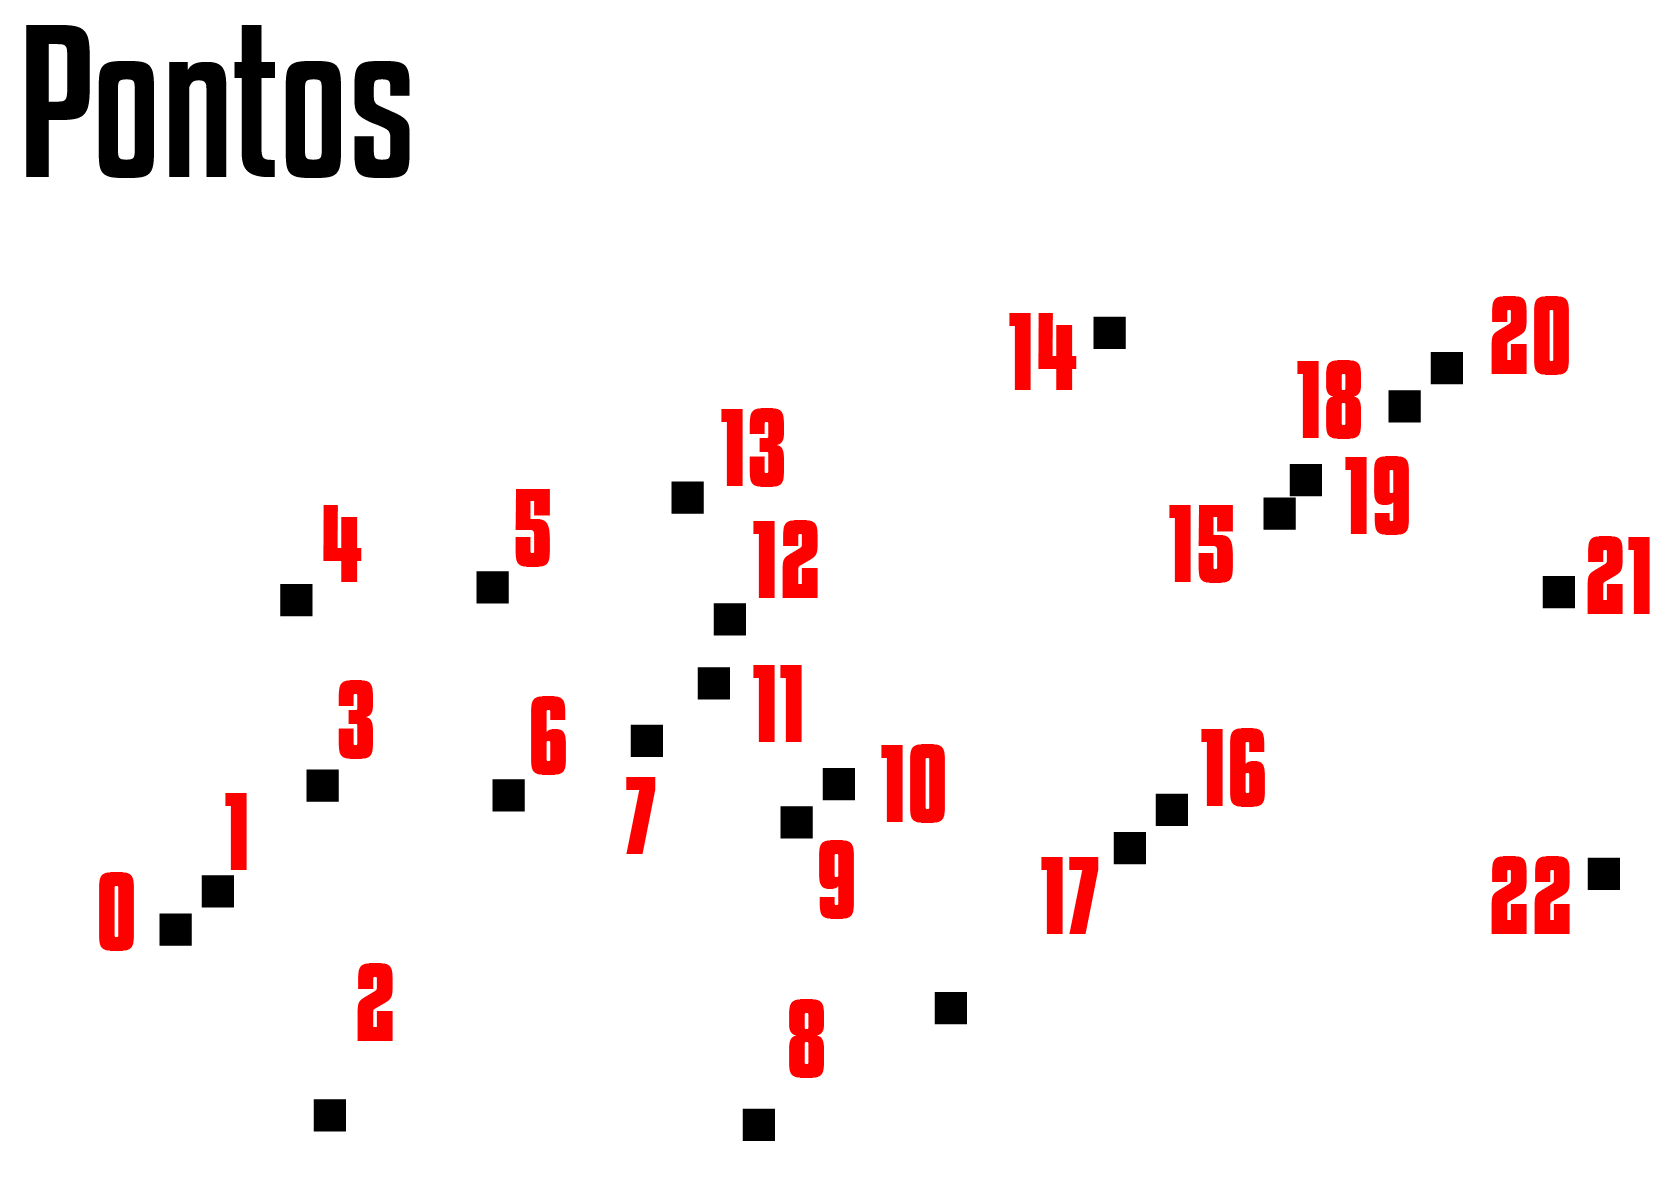
\includegraphics[width=0.5\textwidth]{Figures/WiseElementPoints@16x.png}
	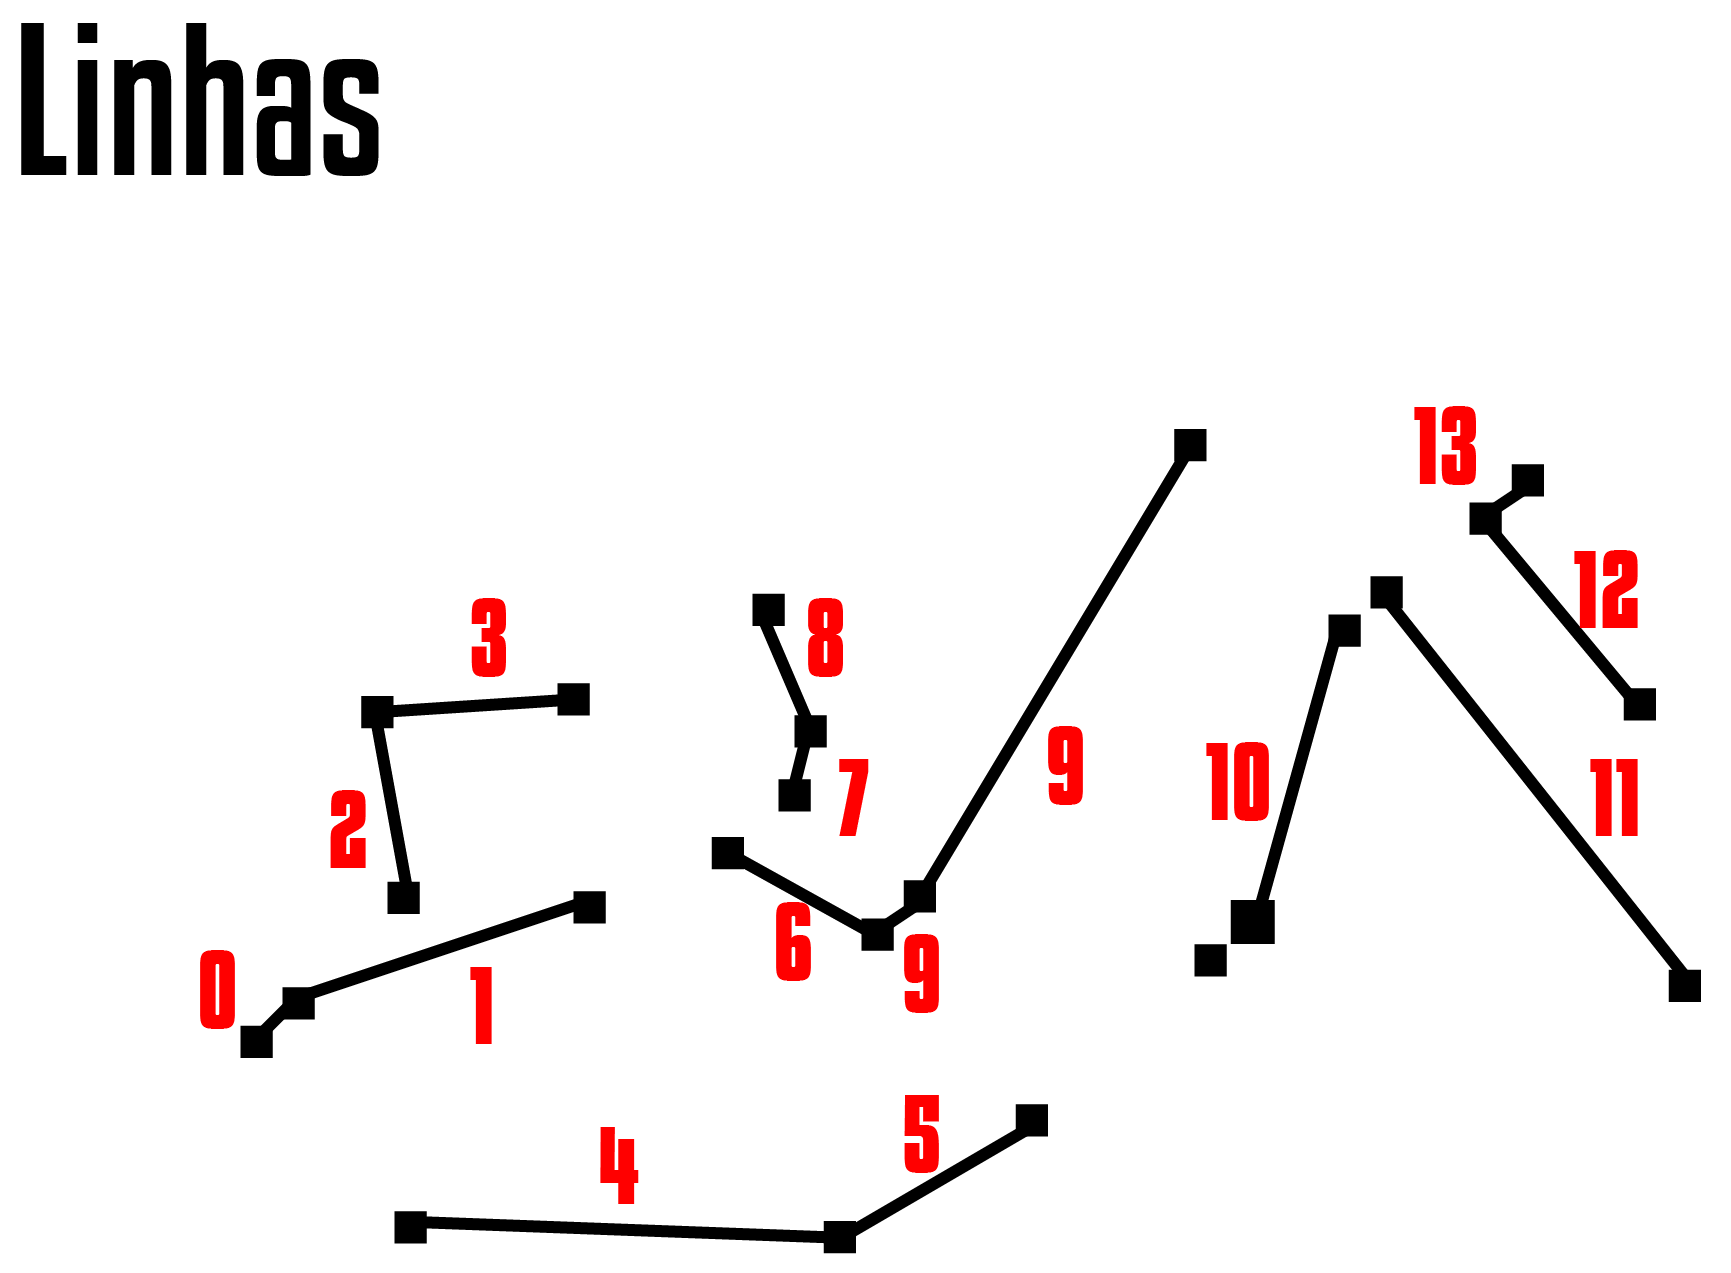
\includegraphics[width=0.5\textwidth]{Figures/WiseElementLines@16x.png}
	
	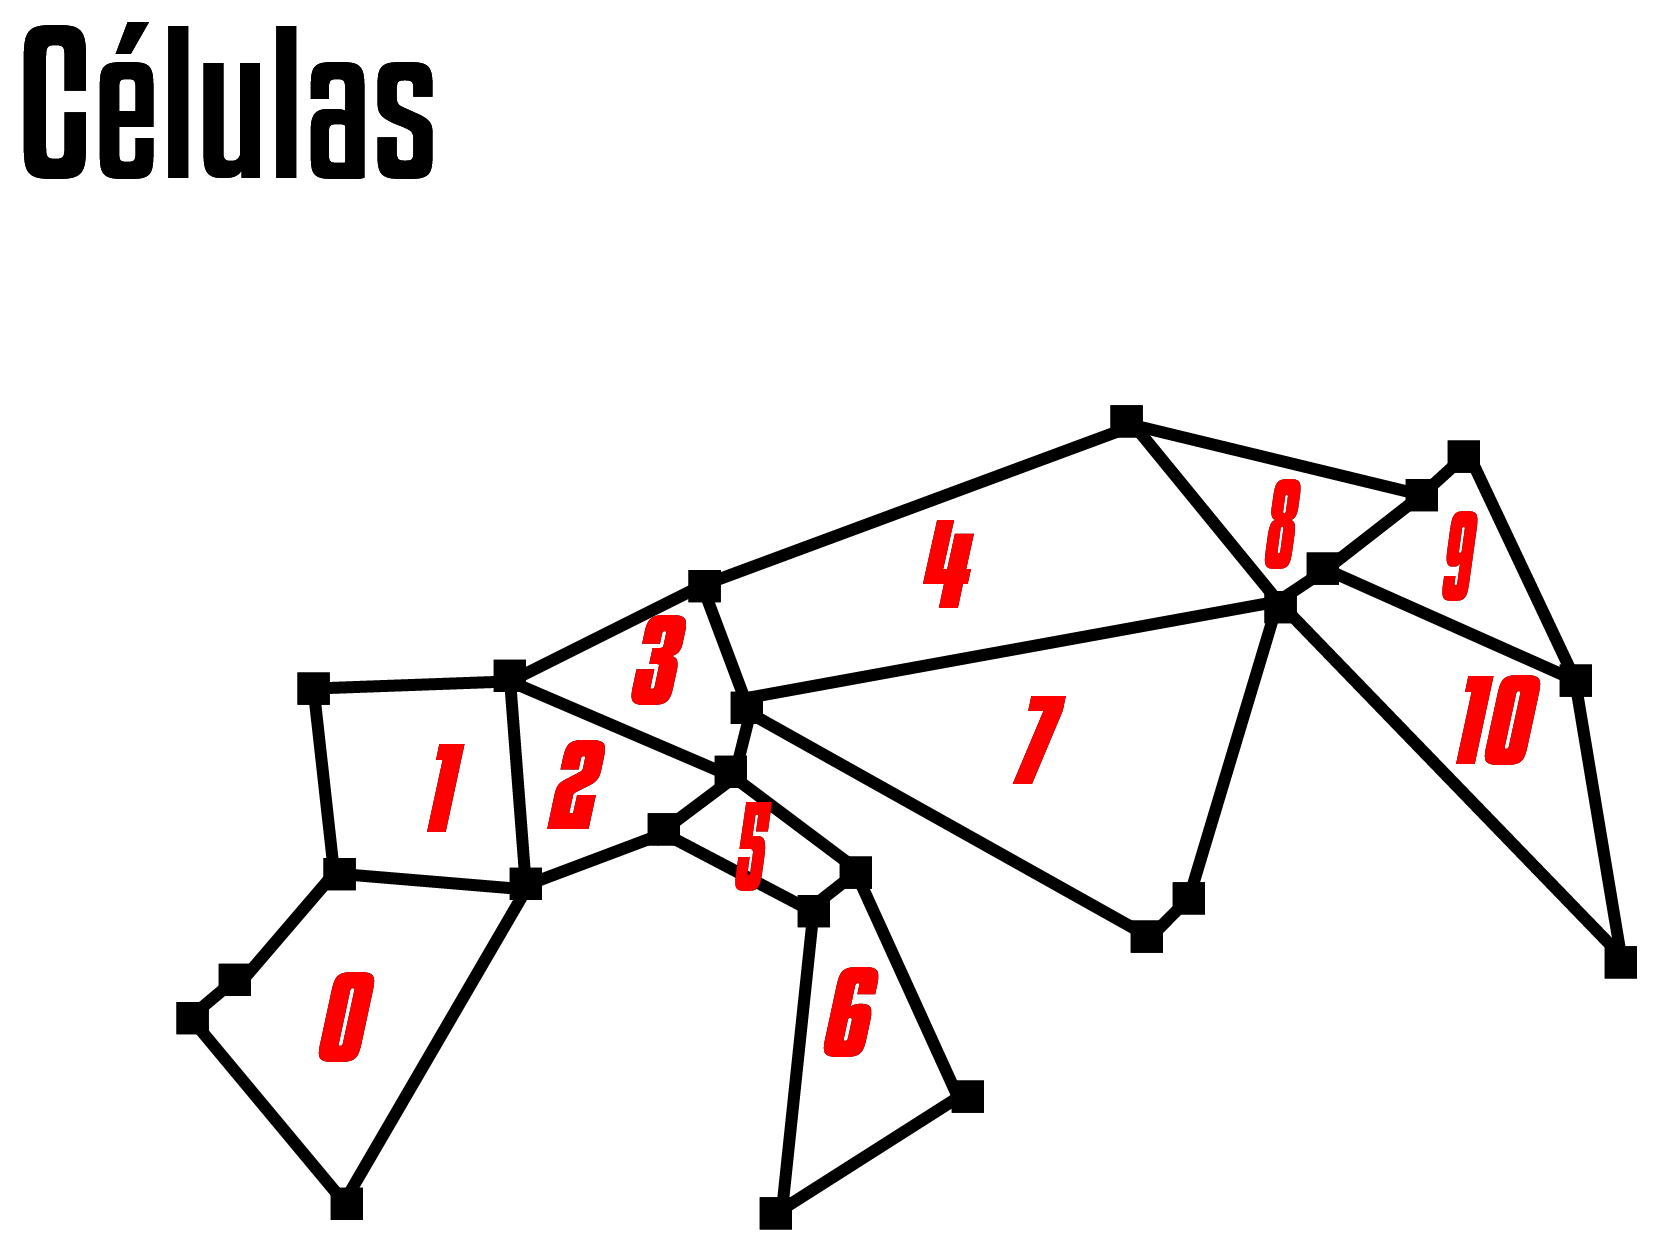
\includegraphics[width=0.5\textwidth]{Figures/WiseElementCells@16x.png}
	\caption{Pontos utilizados na especificação do modelo geométrico. Linhas utilizadas na especificação do modelo geométrico, através dos pontos previamente definidos. Células utilizadas na especificação do modelo geométrico, através dos pontos previamente definidos.}
	\label{fig2:wiselementstructs}
\end{figure}

Os componentes de uma estrutura inteligente são pontos, células, linhas e campos. Pontos demarcam uma posição no espaço, células e linhas representam conjuntos de pontos e os campos são dados gerais da estrutura. Um modelo de pontos e linhas é capaz de representar o mesmo modelo geométrico de uma árvore arterial, basta considerar cada ponto uma bifurcação de vasos e cada segmento de vaso uma linha. Através destes componentes simples é possível armazenar e acessar dados sobre cada segmento. Para dados gerais do modelo, como a frequência $f$, os campos da estrutura inteligente são utilizados.

A classe \textit{WiseElement} foi desenvolvida para construir a estrutura abstrata (\textit{DataStructure}) à partir das informações contidas na estrutura inteligente (\textit{WiseStructure}), desta forma é importante que a estrutura inteligente possa rapidamente ser armazenada e recuperada. O elemento inteligente é o elemento básico do método de iteração, sendo duplicado antes de ser iterado, gerando novas estruturas inteligente e abstrata idênticas. Imediatamente a nova estrutura abstrata \textit{DataStructure} é descartada e os dados contidos na nova estrutura inteligente \textit{WiseStructure} são armazenados. Portanto, a estrutura abstrata não estará sempre presente. Seguindo este ciclo de vida, todos os elementos inteligentes obedecem à máquina de status contida na Figura~\ref{fig3:wiselementstatus}.

\begin{figure}[!htbp]
	\centering
	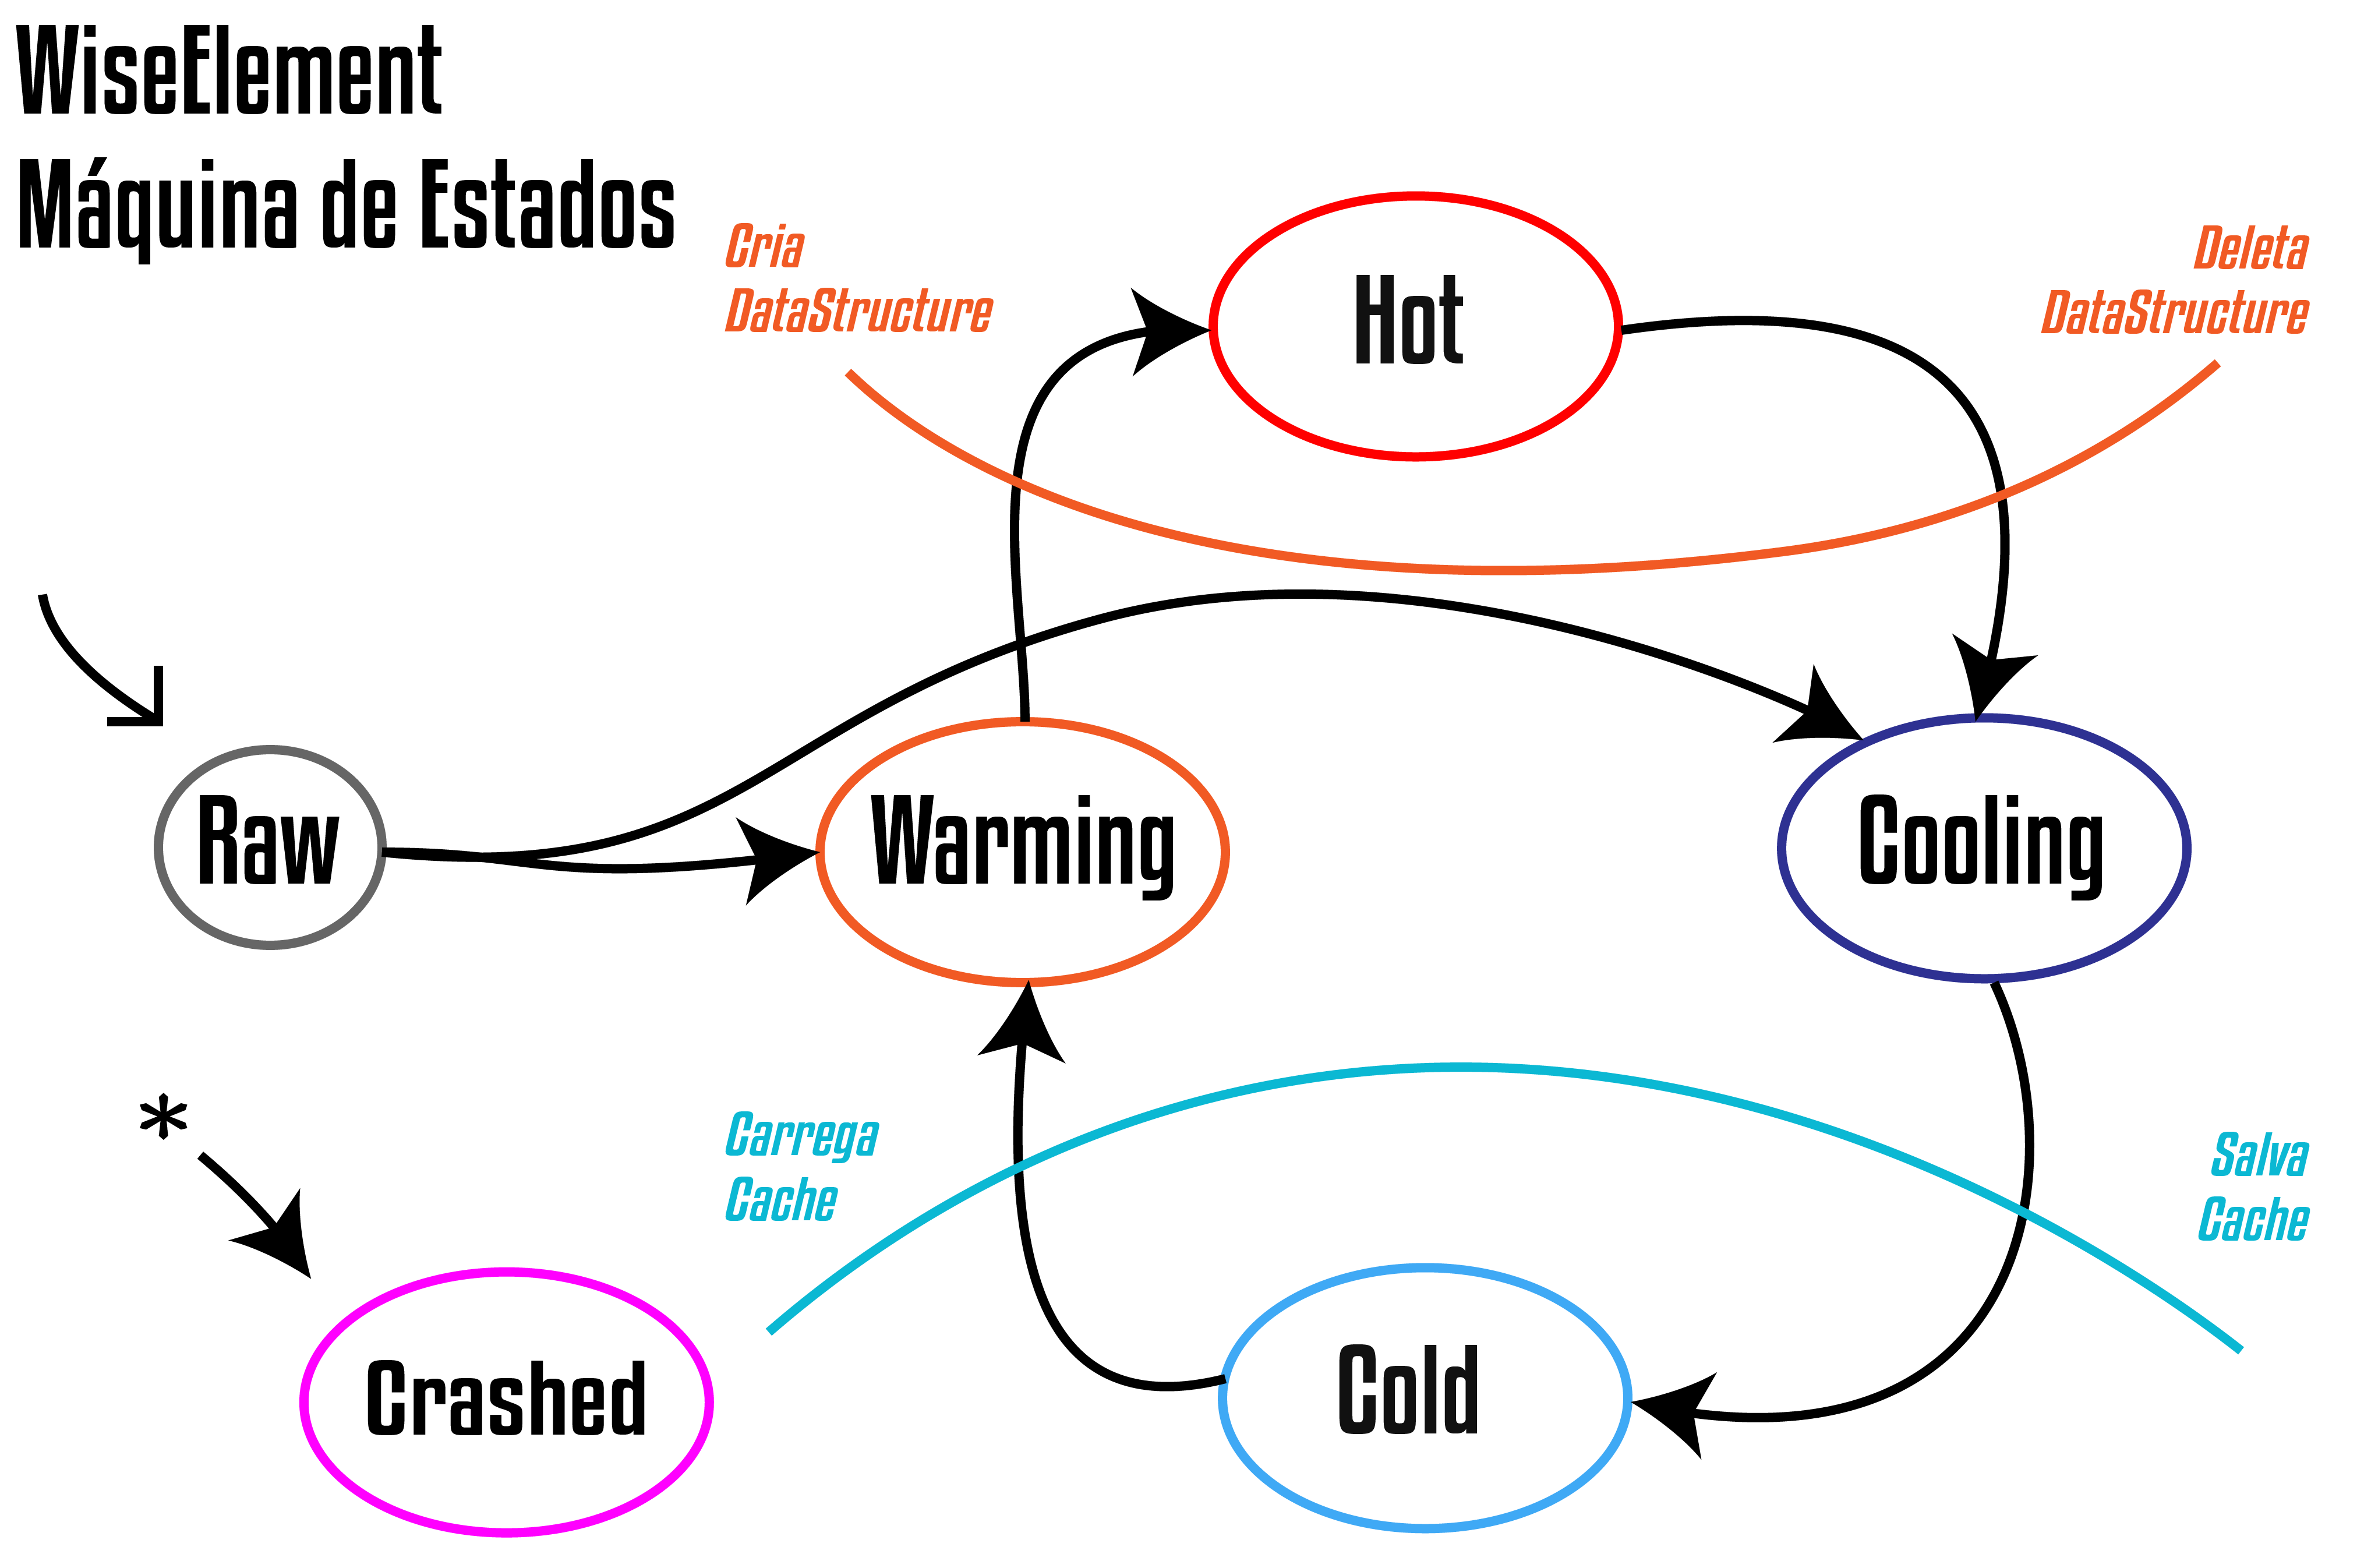
\includegraphics[scale=1.5]{Figures/WiseElementStatus@16x.png}
	\caption{Máquina de estados que controla o funcionamento de um elemento inteligente.}
	\label{fig3:wiselementstatus}
\end{figure}

A máquina de status dos elementos inteligentes gerencia o ciclo de vida de todos os elementos inteligentes, elementos inicialmente recebem o estado \textit{Raw}, ou cru, que representa um elemento ainda sem estruturas carregadas ou sem consistência garantida. Uma vez que a estrutura inteligente é inserida e verificada o elemento muda para o status \textit{Warming} ou \textit{Cooling}, respectivamente esquentando ou esfriando, suas estruturas estão representadas na Figura~\ref{fig4:wiselementwarming}.

\begin{figure}[!htbp]
	\centering
	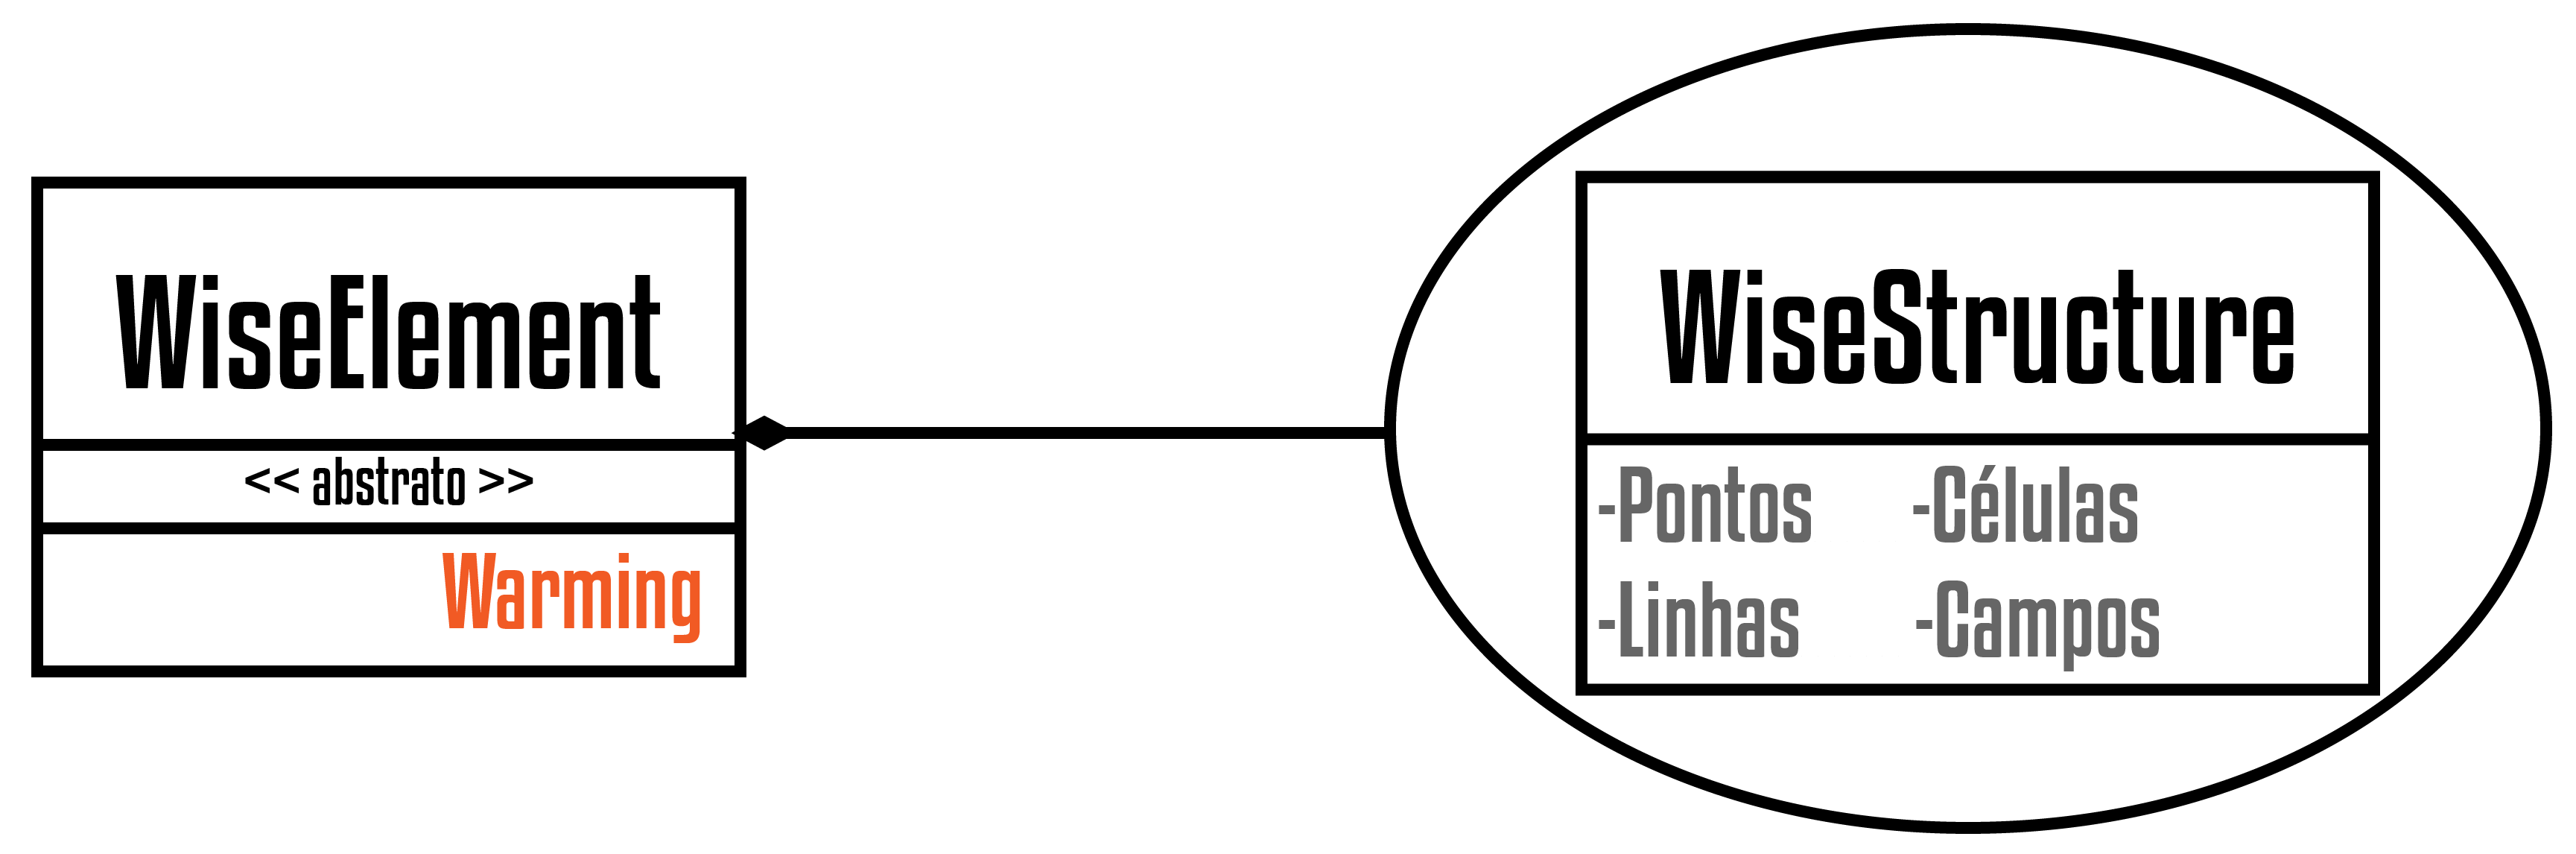
\includegraphics[scale=1.85]{Figures/WiseElementWarming@16x.png}
	\caption{Elemento inteligente enquanto no estado \textit{Warming}.}
	\label{fig4:wiselementwarming}
\end{figure}

A figura~\ref{fig4:wiselementwarming} mostra as estruturas presentes em elementos no estado \textit{Warming} que é a mesma dos estados \textit{Raw} e \textit{Cooling}. Cada estado possui uma finalidade diferente e representa em que estado estão as informações do elemento inteligente. Elementos no estado \textit{Warming} estão aguardando a construção de sua estrutura abstrata, enquanto elementos  no estado \textit{Cooling} aguardam que seus dados sejam salvos em cache. Finalmente, elementos no estado \textit{Raw} indicam que não é esperada a consistência dos dados.

Inicialmente os elementos inteligentes são criados no estado \textit{Raw}, enquanto os dados do elemento são carregados ele permanecerá neste estado. Ao final do carregamento o objeto trocará de estado para \textit{Warming} ou \textit{Cooling}, que indicam o próximo passo do elemento. Estar no estado \textit{Warming} indica que o objetivo é esquentar o objeto, atingindo o estado \textit{Hot}. Enquanto o estado \textit{Cooling} indica que a estrutura inteligente aguarda resfriamento, atingindo o estado \textit{Cold}. Quando os dados abstratos são criados corretamente para o elemento inteligente seu estado é definido como \textit{Hot}, neste estado todas as informações do objeto estão em memória, sendo este o estado mais pesado do elemento inteligente. Em contraponto, o estado \textit{Cold} indica que a estrutura inteligente foi corretamente armazenada em disco, elementos inteligentes neste estado estão em seu estado mais leve, pois possuem em memória apenas o caminho para a estrutura inteligente armazenada.

Como demonstrado na figura~\ref{fig3:wiselementstatus}, o estado frio (\textit{Cold}) está associado com o uso de um cache para estruturas inteligentes. A estrutura do arquivo é equivalente à uma malha estruturada VTK, mas são efetivamente salvos em um arquivo \textit{XML}. Caso sejam novamente carregados por uma mudança de estado ou deletados o arquivo armazenado é deletado. 

\begin{figure}[!htbp]
	\centering
	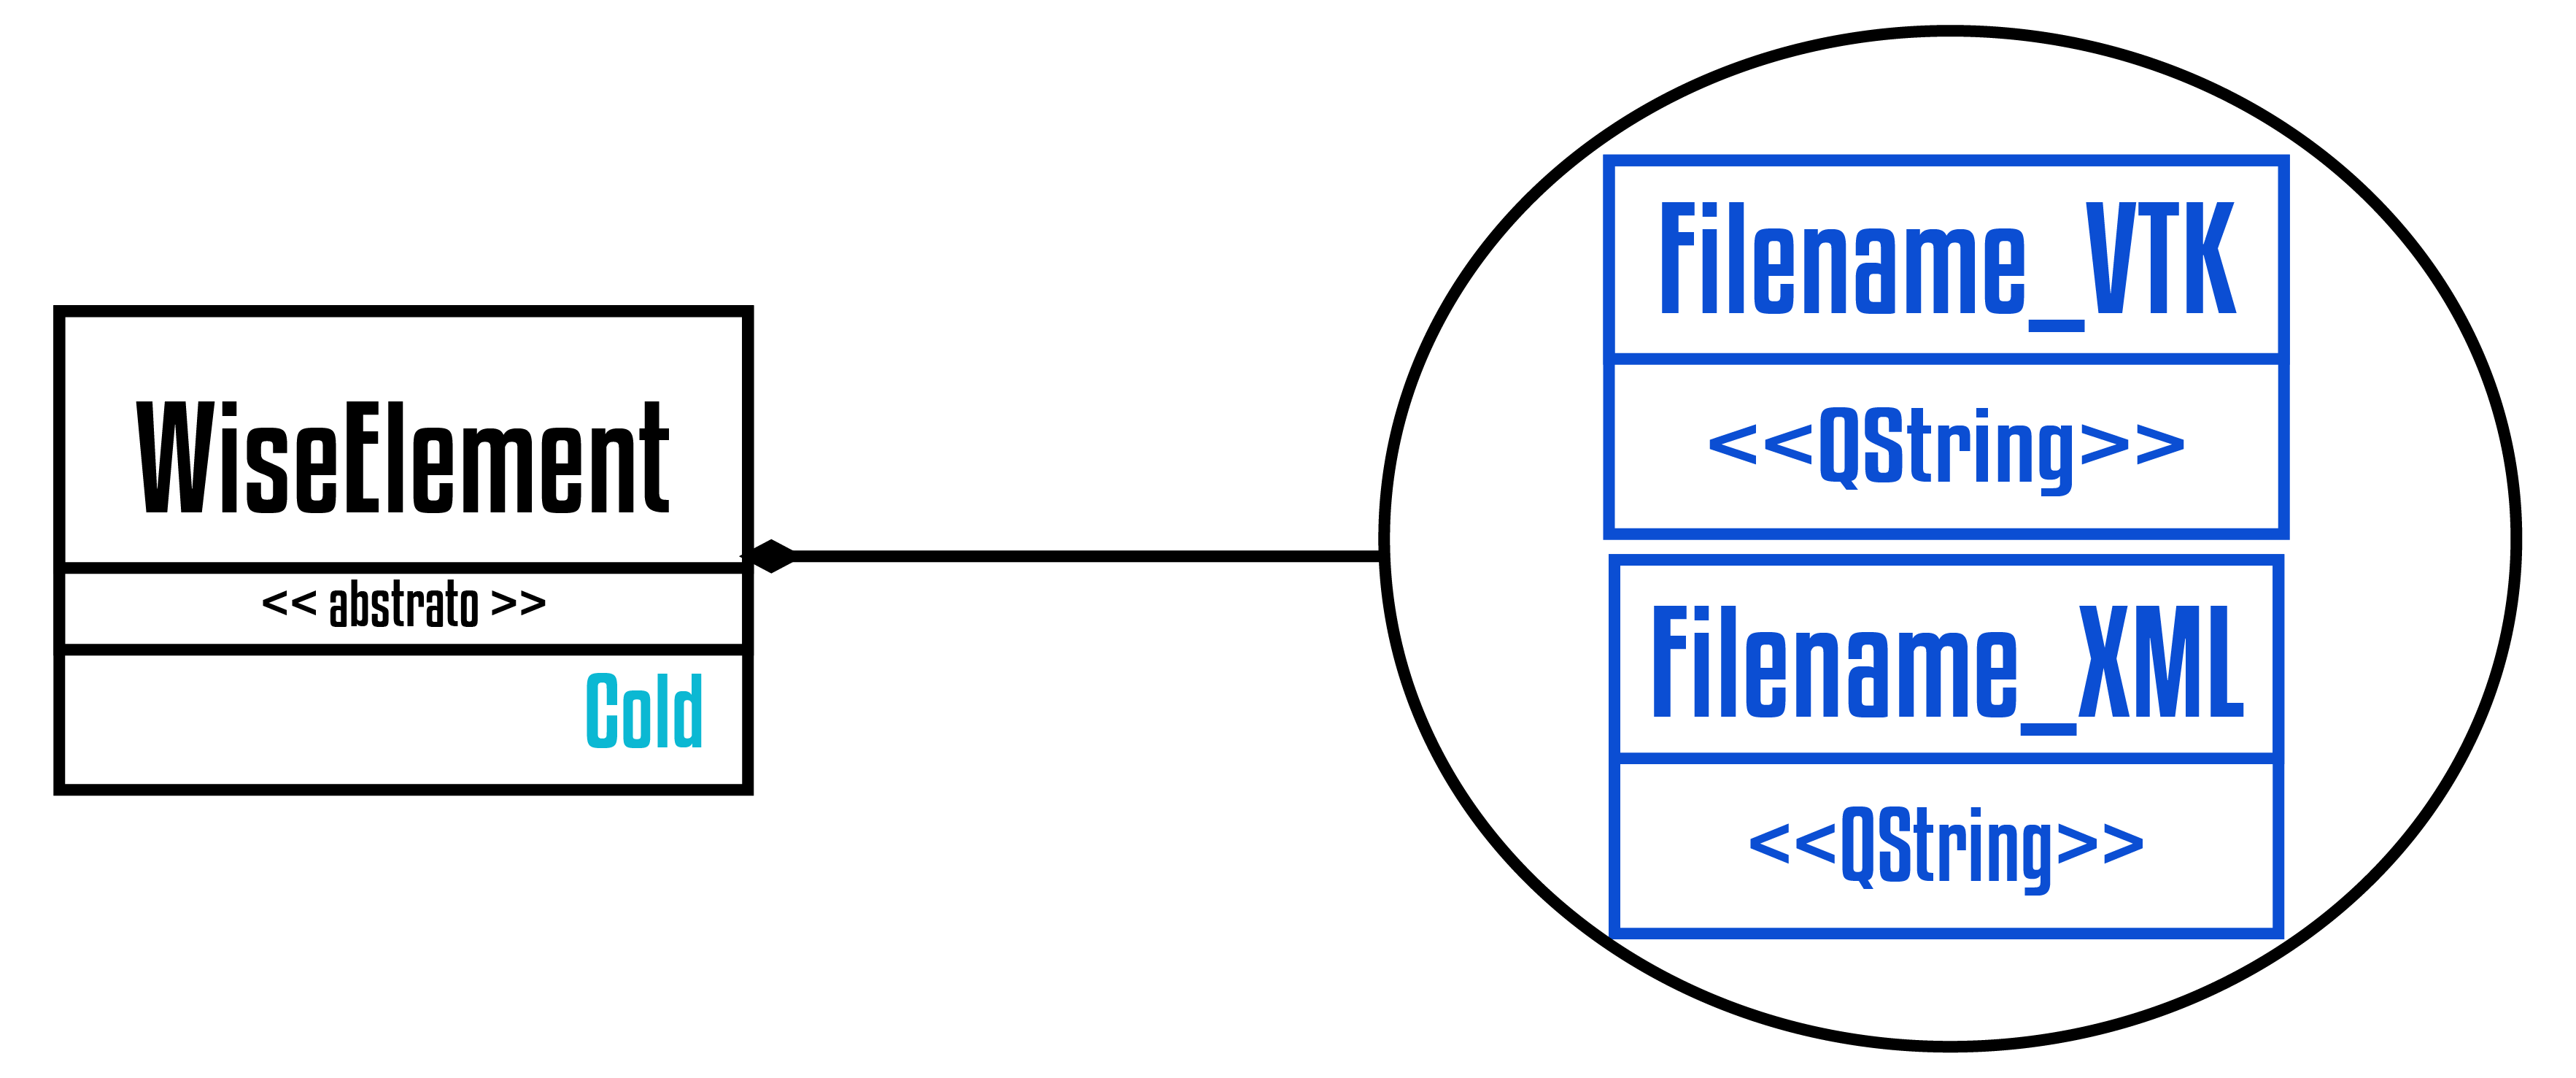
\includegraphics[scale=1.85]{Figures/WiseElementCold@16x.png}
	\caption{Elemento inteligente enquanto no estado \textit{Cold}.}
	\label{fig5:wiselementcold}
\end{figure}

O estado \textit{Crashed} serve para identificar objetos que não tem mais o funcionamento esperado. Durante a troca de estados do elemento é verificado se as estruturas esperadas estão presentes, caso não estejam o objeto é direcionado à este estado.

Finalmente, o estado \textit{Hot} representa os elementos que possuem todas as estruturas presentes. Isto significa que a estrutura inteligente \textit{WiseStructure} e a estrutura abstrata equivalente \textit{DataStructure} estão presentes e são consistentes.

\begin{figure}[!htbp]
	\centering
	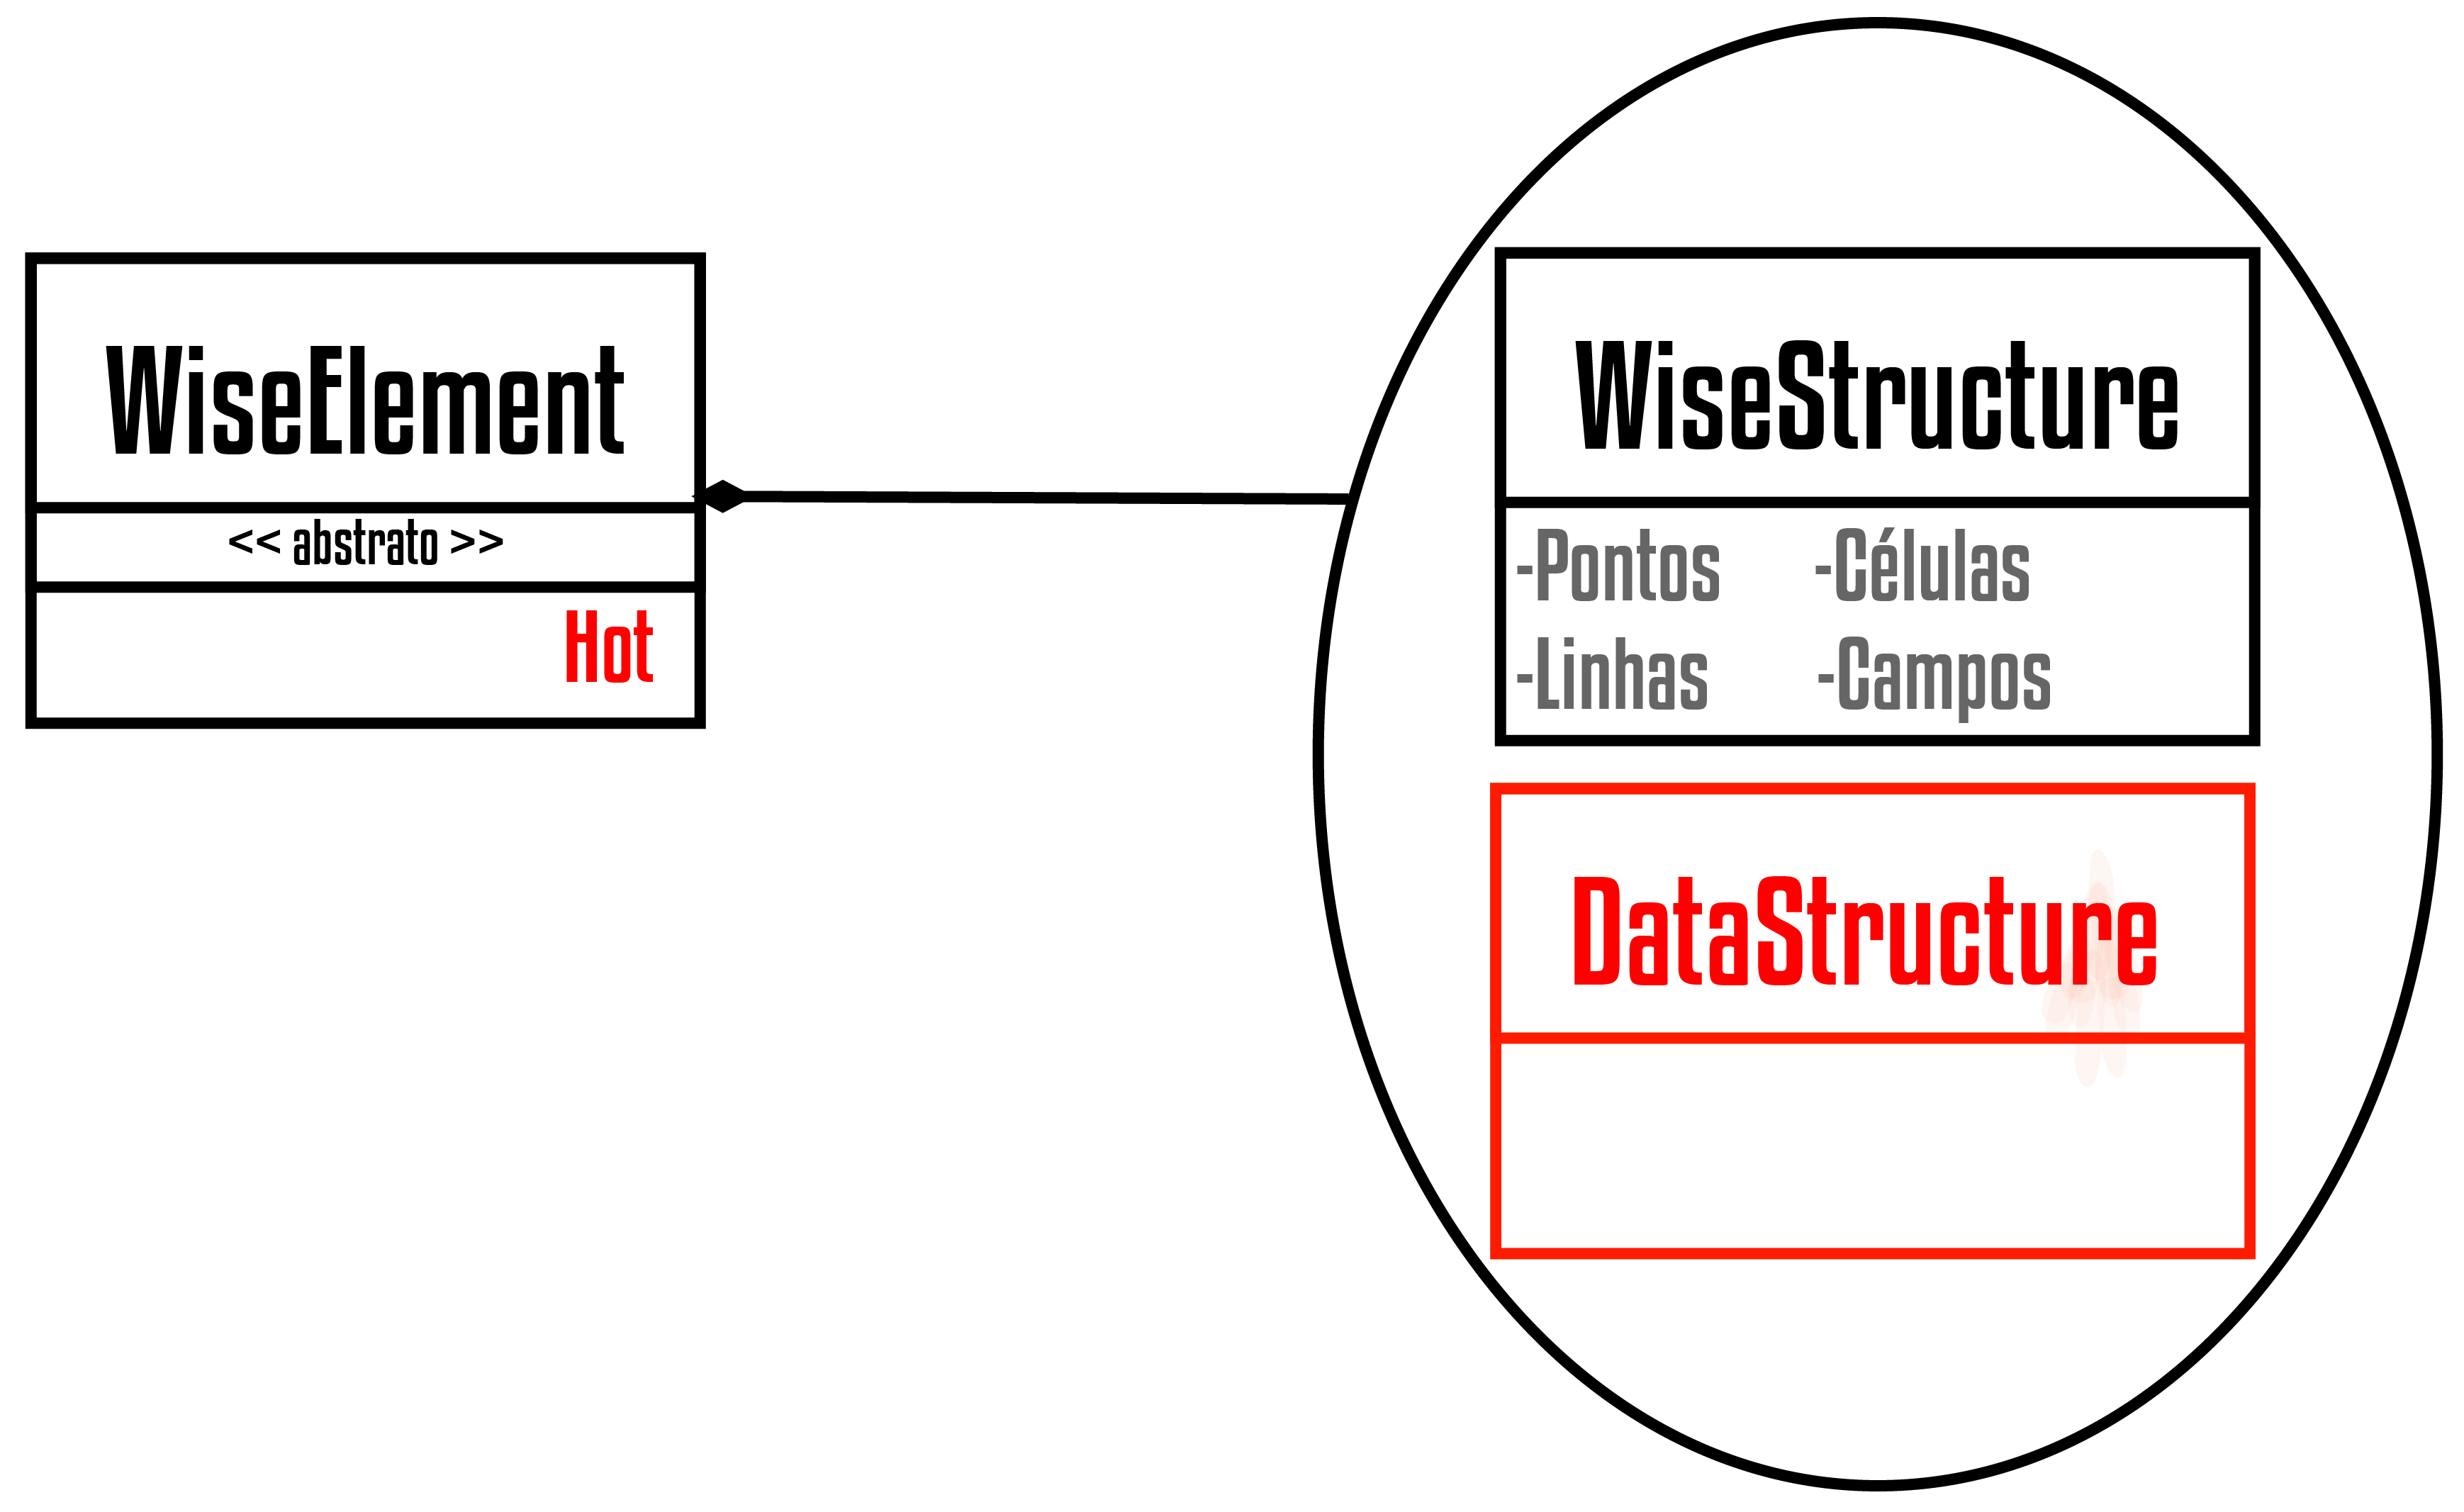
\includegraphics[scale=1.85]{Figures/WiseElementHot@16x.png}
	\caption{Elemento inteligente enquanto no estado \textit{Hot}.}
	\label{fig6:wiseelementhot}
\end{figure}

Para que um elemento possa ser iterado ele precisa estar no estado \textit{Hot}, porque durante a iteração de um elemento inteligente seus dados abstratos são utilizados. A cada passo da iteração a estrutura \textit{DataStructure} é atualizada, exigindo uma atualização da estrutura \textit{WiseStructure}.

Seguindo o conceito de classes com propósito único, os elementos inteligentes são responsáveis apenas por gerir os dados contidos na estrutura inteligente e abstrata. Portanto as funções de criar, iterar e visualizar estas estruturas foram divididas em outras classes.

%--------------------------------------------------------------------------------%
\subsection{FÁBRICA}\label{sec:fabrica} 

Como mencionado anteriormente três principais barreiras foram identificadas armazenamento, iteração e visualização. Nesta seção uma arquitetura de classes que permite a execução de cada passo através do paradigma de Fábricas Dinâmicas~ \cite{factorypattern} é proposta. Uma arquitetura com fábricas permite a criação de instâncias com definições concretas, armazenadas como metadados. Isso facilita a adição de novos objetos que podem ser interpretados sem modificar o código da fábrica em si. Sendo a fábrica também uma classe virtual, três principais tipos de fábricas foram idealizadas, a primeira responsável por criar elementos inteligentes, a  segunda responsável por iterar o elemento e a terceira que cria um elemento gráfico a partir de um elemento inteligente.

\begin{figure}[!htbp]
	\centering
	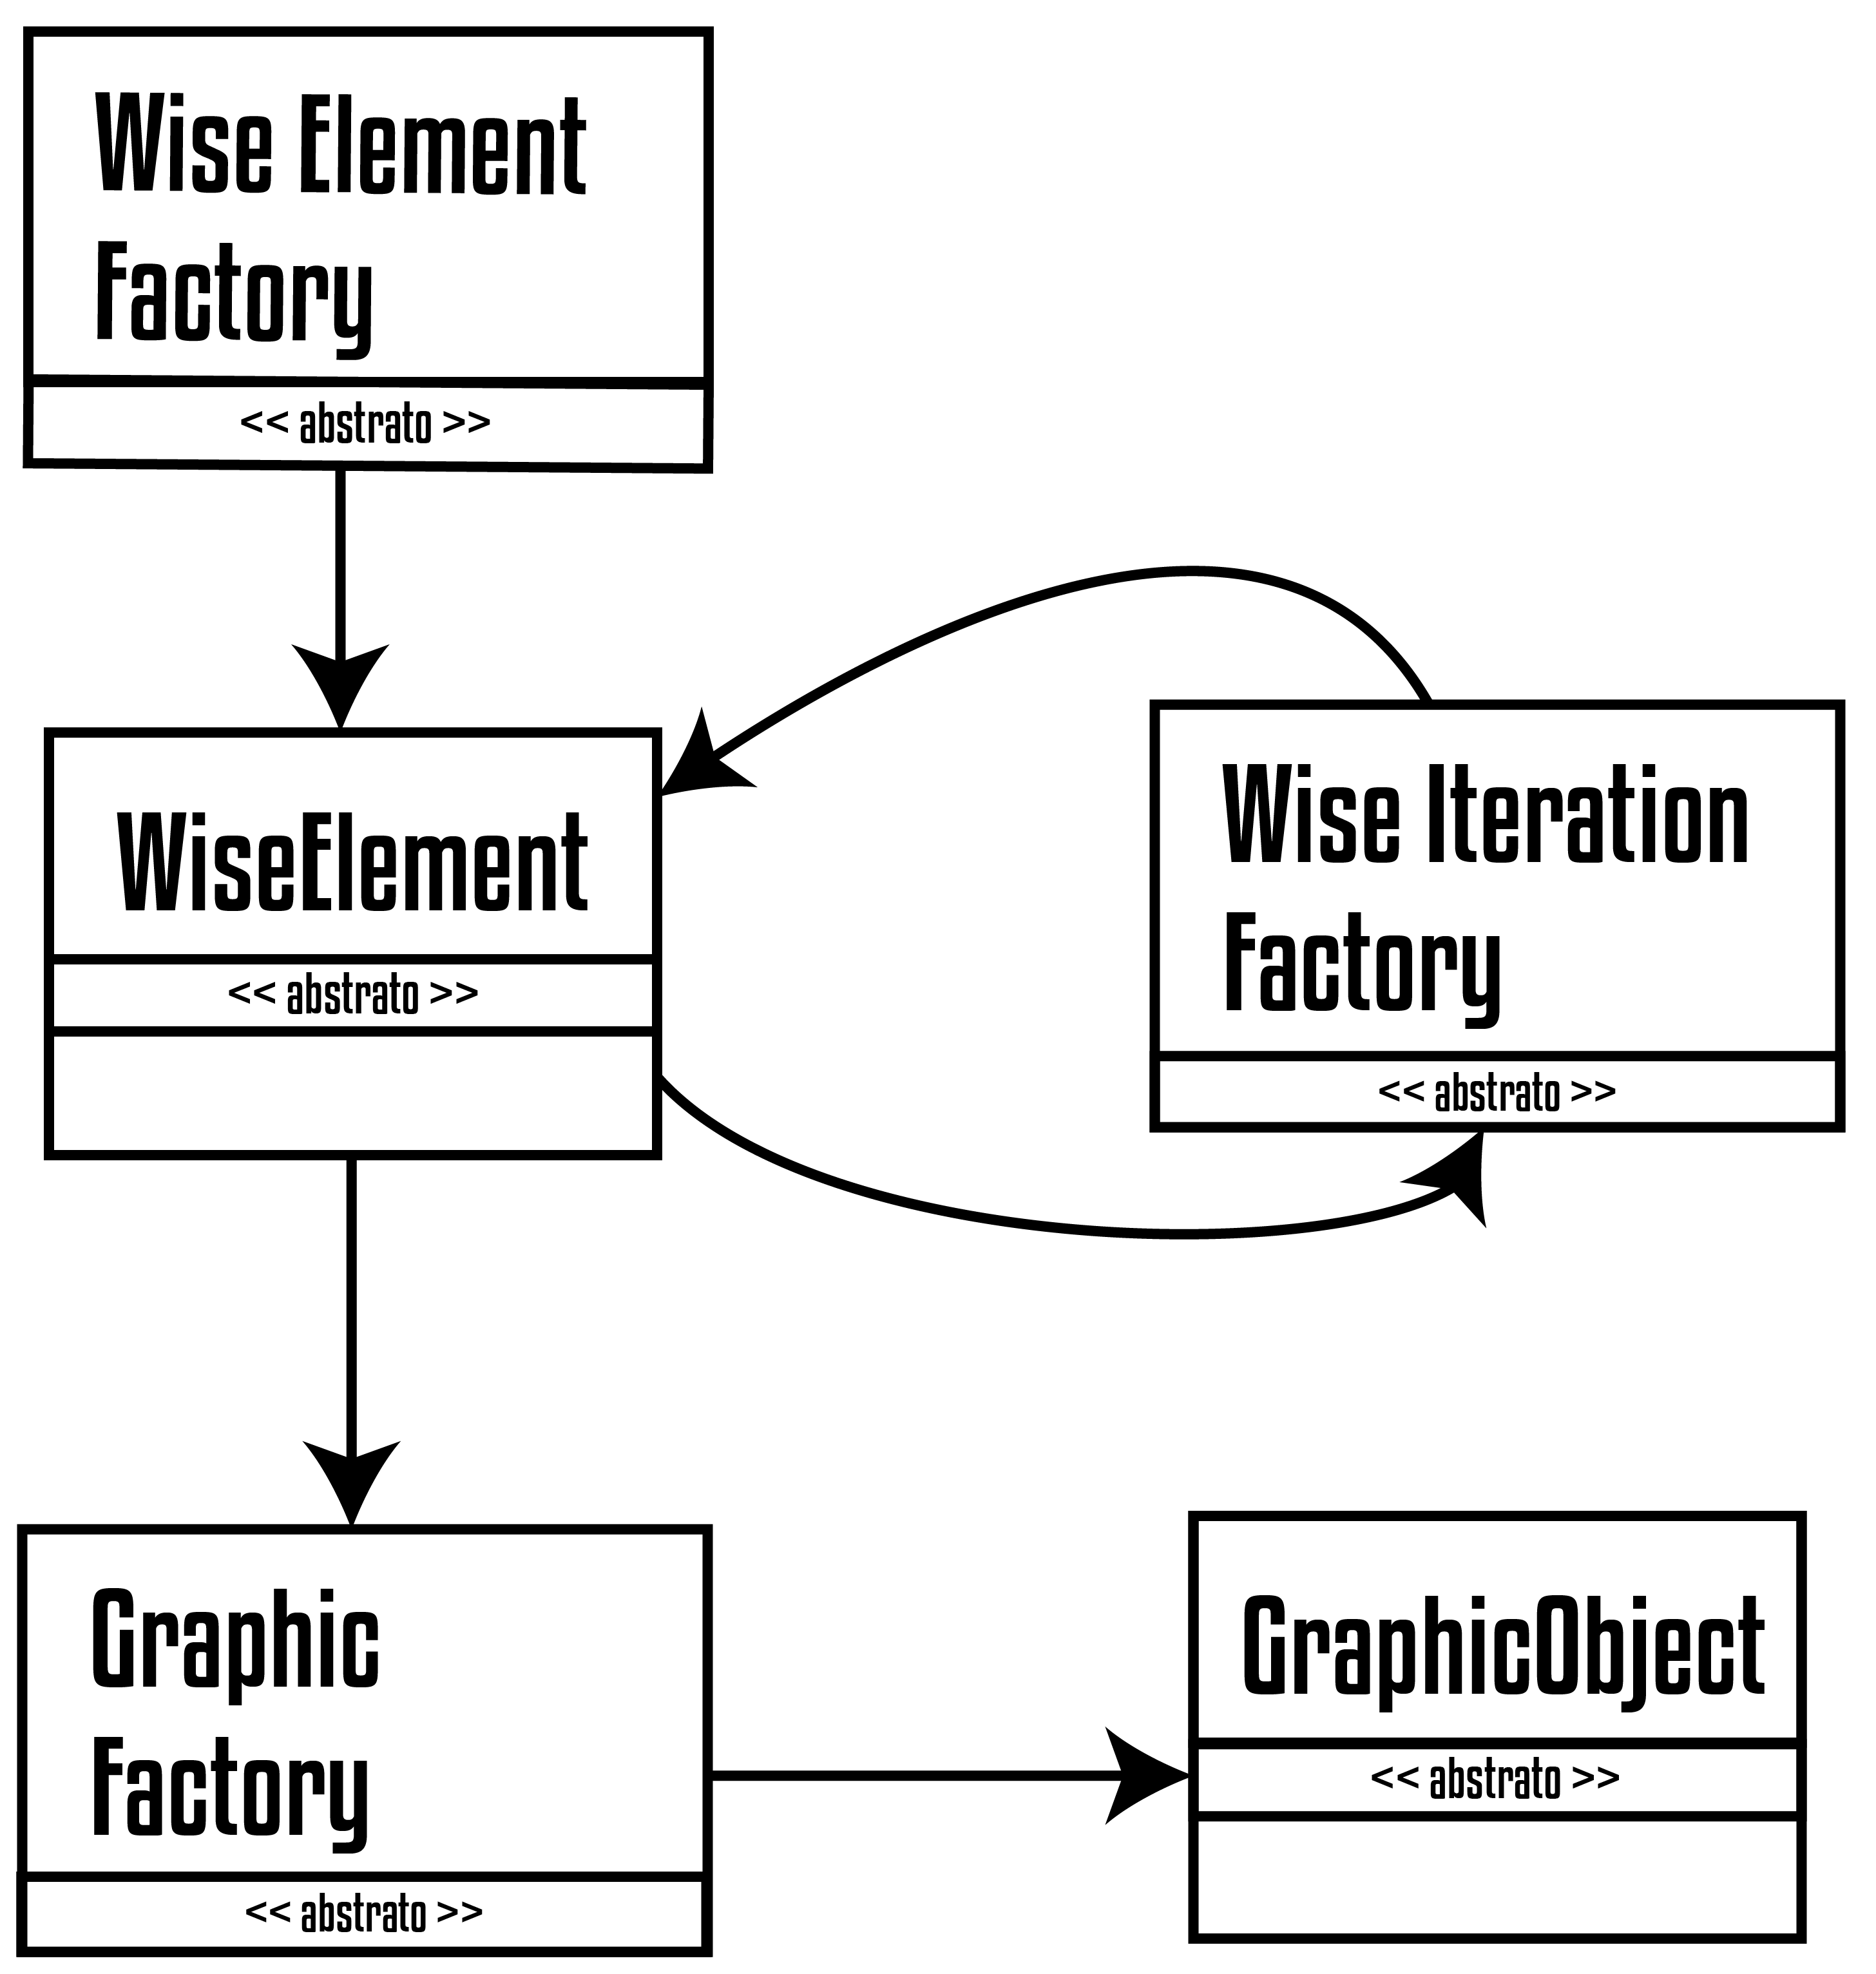
\includegraphics[width=0.75\textwidth]{Figures/WiseElementWorkflow@16x.png}
	\caption{Arquitetura de classes fábrica e fluxo de trabalho do elemento inteligente WiseElement. A fábrica WiseElementFactory é responsável por criar o elementos inteligentes, a fábrica WiseIterationFactory é reponsável pela iteração do elemento inteligente e a fábrica GraphicFactory é responsável por criar as estrturas de visualização. }
	\label{fig2:wiselementsworkflow}
\end{figure}

Primeiramente, a fábrica de elementos inteligentes \textit{WiseElementFactory} é utilizada para a criação de elementos inteligentes, essa fábrica é utilizada para criar um elemento inteligente à partir de parâmetros pré-definidos. Esse tipo de fábrica é também uma classe virtual, seus métodos definem que fábricas de elementos inteligentes possuem três maneiras de executar: Um dos métodos permite a criação de elementos à partir de uma lista de exemplos; Outro método cria um elemento com um arquivo \textit{VTK} ; E, um último que recebe um arquivo \textit{XML} como entrada.

Os métodos de criação de elementos são selecionados através do nome da fábrica e de um dos três métodos de criação. A ferramenta computacional possui uma lista com todas a fábricas disponíveis e as utiliza quando necessário. Devido à forma como os dados são carregados para cada elemento, é necessário que haja uma fábrica para cada tipo de elemento inteligente.

Similarmente, a fábrica \textit{WiseIterationFactory} só pode operar com um tipo específico de elemento inteligente, entretanto é possível que haja mais de uma fábrica de iteração disponível por tipo de elemento inteligente. Desta forma uma árvore arterial pode ser iterada por diferente algoritmos de iteração e o mesmo ocorre com os outros tipos de elementos. Estas fábricas são responsáveis por executar algum algoritmo que utilize o tipo de dados do elemento inteligente. No caso de uma árvore arterial é possível utilizar uma fábrica que irá executar o modelo matemático descrito na Seção~\ref{sec:algoritmo} utilizando os ponteiros para segmentos disponíveis em uma \textit{WiseArteryTree}.

Por último, a fábrica \textit{GraphicFactory} irá criar o objeto gráfico correspondente ao elemento inteligente. Assim como um elemento inteligente um objeto gráfico pode ser salvo em cache.  Um elemento inteligente é composto por todas as linhas, pontos, células e seus valores associados, enquanto um objeto gráfico contém as representações gráficas destas estruturas e permite a visualização destes valores associados. Os elementos estruturais de uma árvore arterial, que são seus pontos e linhas, são traduzidos em esferas e cilindros como visto na Figura~\ref{fig1:gui}. A cor destas esferas e cilindros representam algum valor associado à estrutura, apenas um valor pode ser exibido por vez ao longo da escala de cores, como o fluxo $Q$ ou a pressão $P$. Desta forma os elementos gráficos só exigem que um parâmetro por vez seja armazenado.


%--------------------------------------------------------------------------------%
\subsection{OBJETO INTELIGENTE}\label{sec:objeto_inteligente}

A classe que combina todas as estruturas utilizadas no método de iteração da ferramenta computacional foi nomeada de objeto inteligente \textit{WiseObject}, este objeto preserva todos os passos de de iteração e poupa a quantidade de recursos mantida em memória. A classe é composta por um coleção de elementos inteligentes e objetos gráficos equivalentes entre si. A presença de uma fábrica gráfica é opcional, possibilitando que objetos sejam iterados sem que alguma estrutura seja disponibilizada para visualização. Utilizando a mesma separação de classes com propósito único, fábricas dinâmicas garantem que um objeto inteligente seja criado corretamente. As fábricas presentes na Seção~\ref{sec:fabrica} foram incluídas como propriedades de um objeto inteligente, desta forma estes objetos serão compostos por três fábricas.

O ciclo de vida de um objeto inteligente consiste na sua criação, a iteração de um modelo matemático e, opcionalmente, a exibição de um modelo gráfico. Objetos inteligentes são criados com seu primeiro elemento inteligente. Ao criar um objeto inteligente, sua fábrica adiciona em sua estrutura a fábrica de elementos inteligentes, desta forma objetos inteligentes são capazes de replicar seus elementos inteligentes. No momento da criação, o primeiro elemento é duplicado e uma instância segue para o \textit{Forno}, enquanto a outro segue para o \textit{Freezer}.

O elemento inteligente guardado no \textit{Forno} será o objeto utilizado pelo algoritmo a cada iteração, portanto é sempre o mais recente. A cada ciclo iterativo o elemento contido no \textit{Forno} é duplicado e uma nova instância é adicionada ao \textit{Freezer}, estes elementos aguardam armazenamento.

\begin{figure}[!htbp]
	\centering
	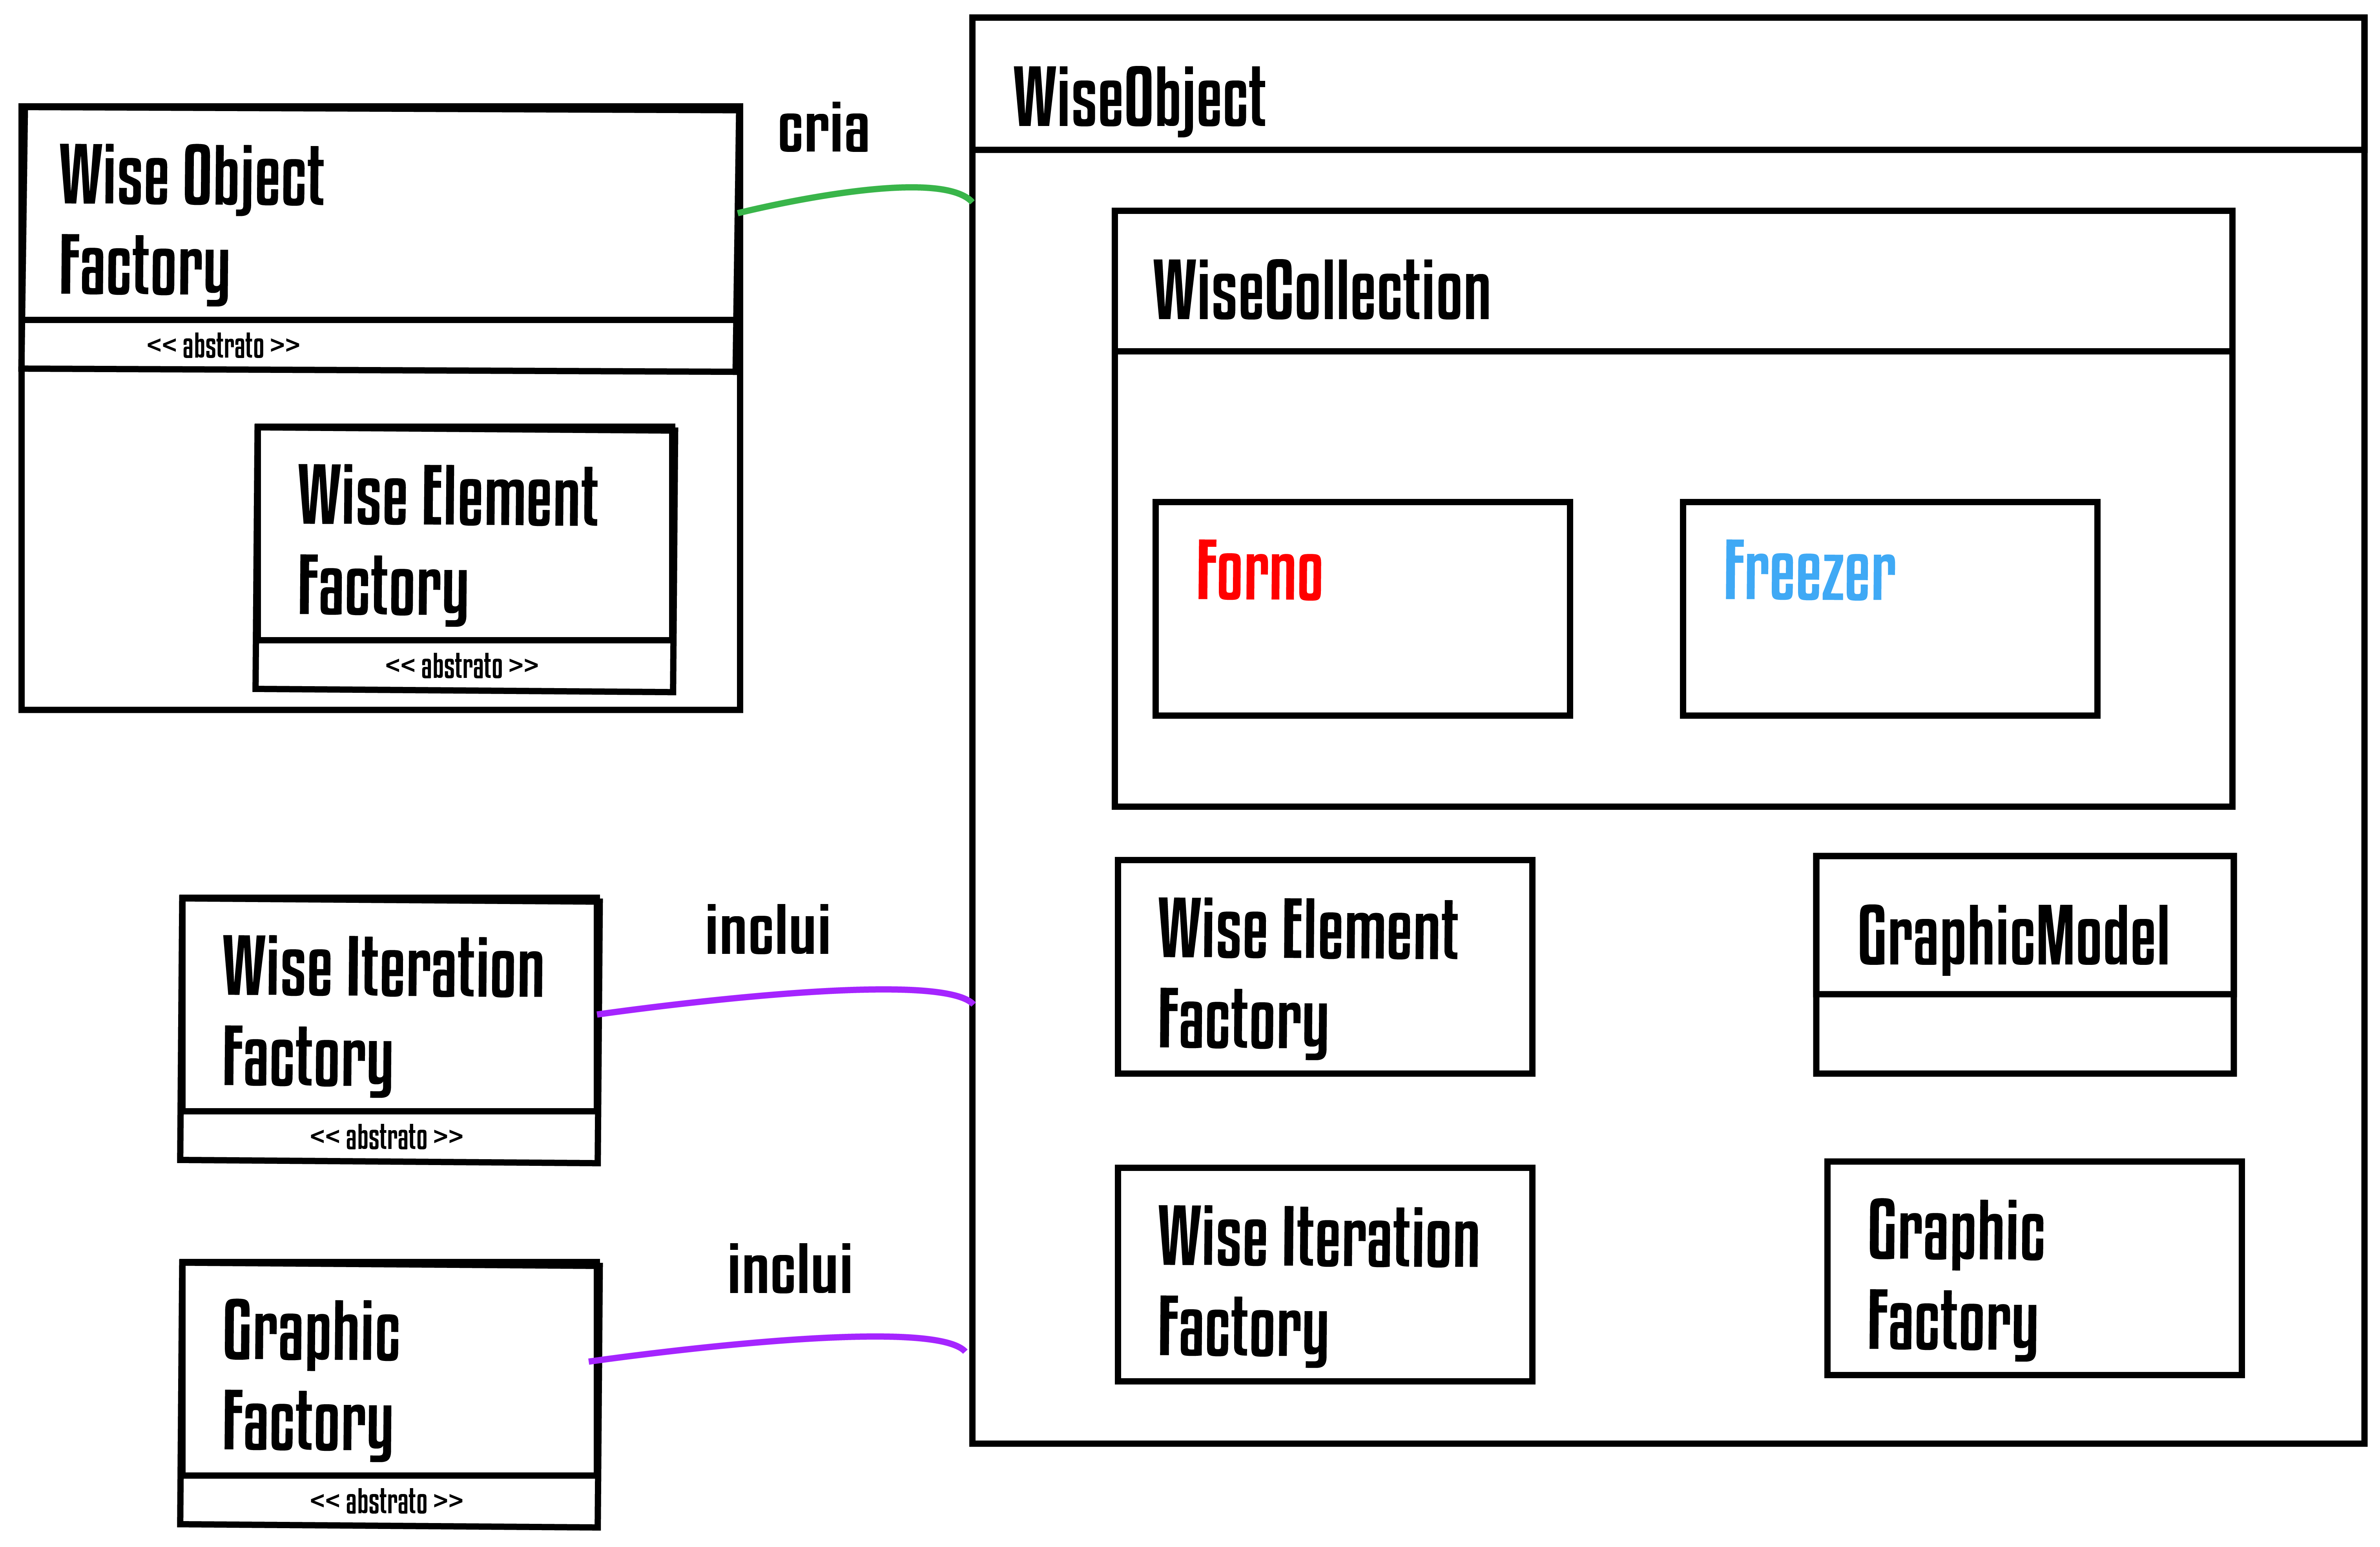
\includegraphics[scale=1.15]{Figures/WiseObject@16x.png}
	\caption{Objeto inteligente \textit{WiseObject} e todos seu componentes:\textit{WiseObjectFactory}, fábrica responsável pela criação de objetos inteligentes; \textit{WiseElementFactory}, fábrica responsável pela criação de elementos inteligentes; \textit{WiseIterationFactory}, fábrica de iteração; \textit{WiseGraphicFactory}, fábrica gráfica; \textit{WiseCollection}, coleção de elementos inteligentes; \textit{GraphicModel}, coleção de objetos gráficos.}
	\label{fig7:wiseobject}
\end{figure}

Através do modelo de classes de um objeto inteligente presente na Figura~\ref{fig7:wiseobject} é possível identificar todos os componentes presentes em um objeto inteligente. O objeto inteligente troca seus elementos de estado automaticamente, a coleção de elementos inteligentes \textit{WiseCollection} irá manter apenas um elemento em memória, o elemento contido no \textit{Forno} que deve permanecer no estado \textit{Hot}. Ao mesmo tempo a coleção irá manter um históricos de elementos armazenados no \textit{Freezer} que devem permanecer no estado \textit{Cold}. É possível que o objeto inteligente volte à um estado anterior, substituindo o elemento presente no \textit{Forno} com algum estado anterior armazenado no \textit{Freezer}, dessa forma o elemento inteligente utilizado no método iterativo será o objeto recuperado. Ao realizar essa operação, a coleção de elementos inteligentes irá recuperar a estrutura inteligente do elemento, alterando seu estado para \textit{Warming}, em seguida irá recriando seus dados abstratos utilizando a fábrica de elementos inteligentes disponível, alterando seu estado para \textit{Hot}. Estas mudanças de estados são descritas pela máquina de estados do objeto inteligente.

\begin{figure}[!htbp]
	\centering
	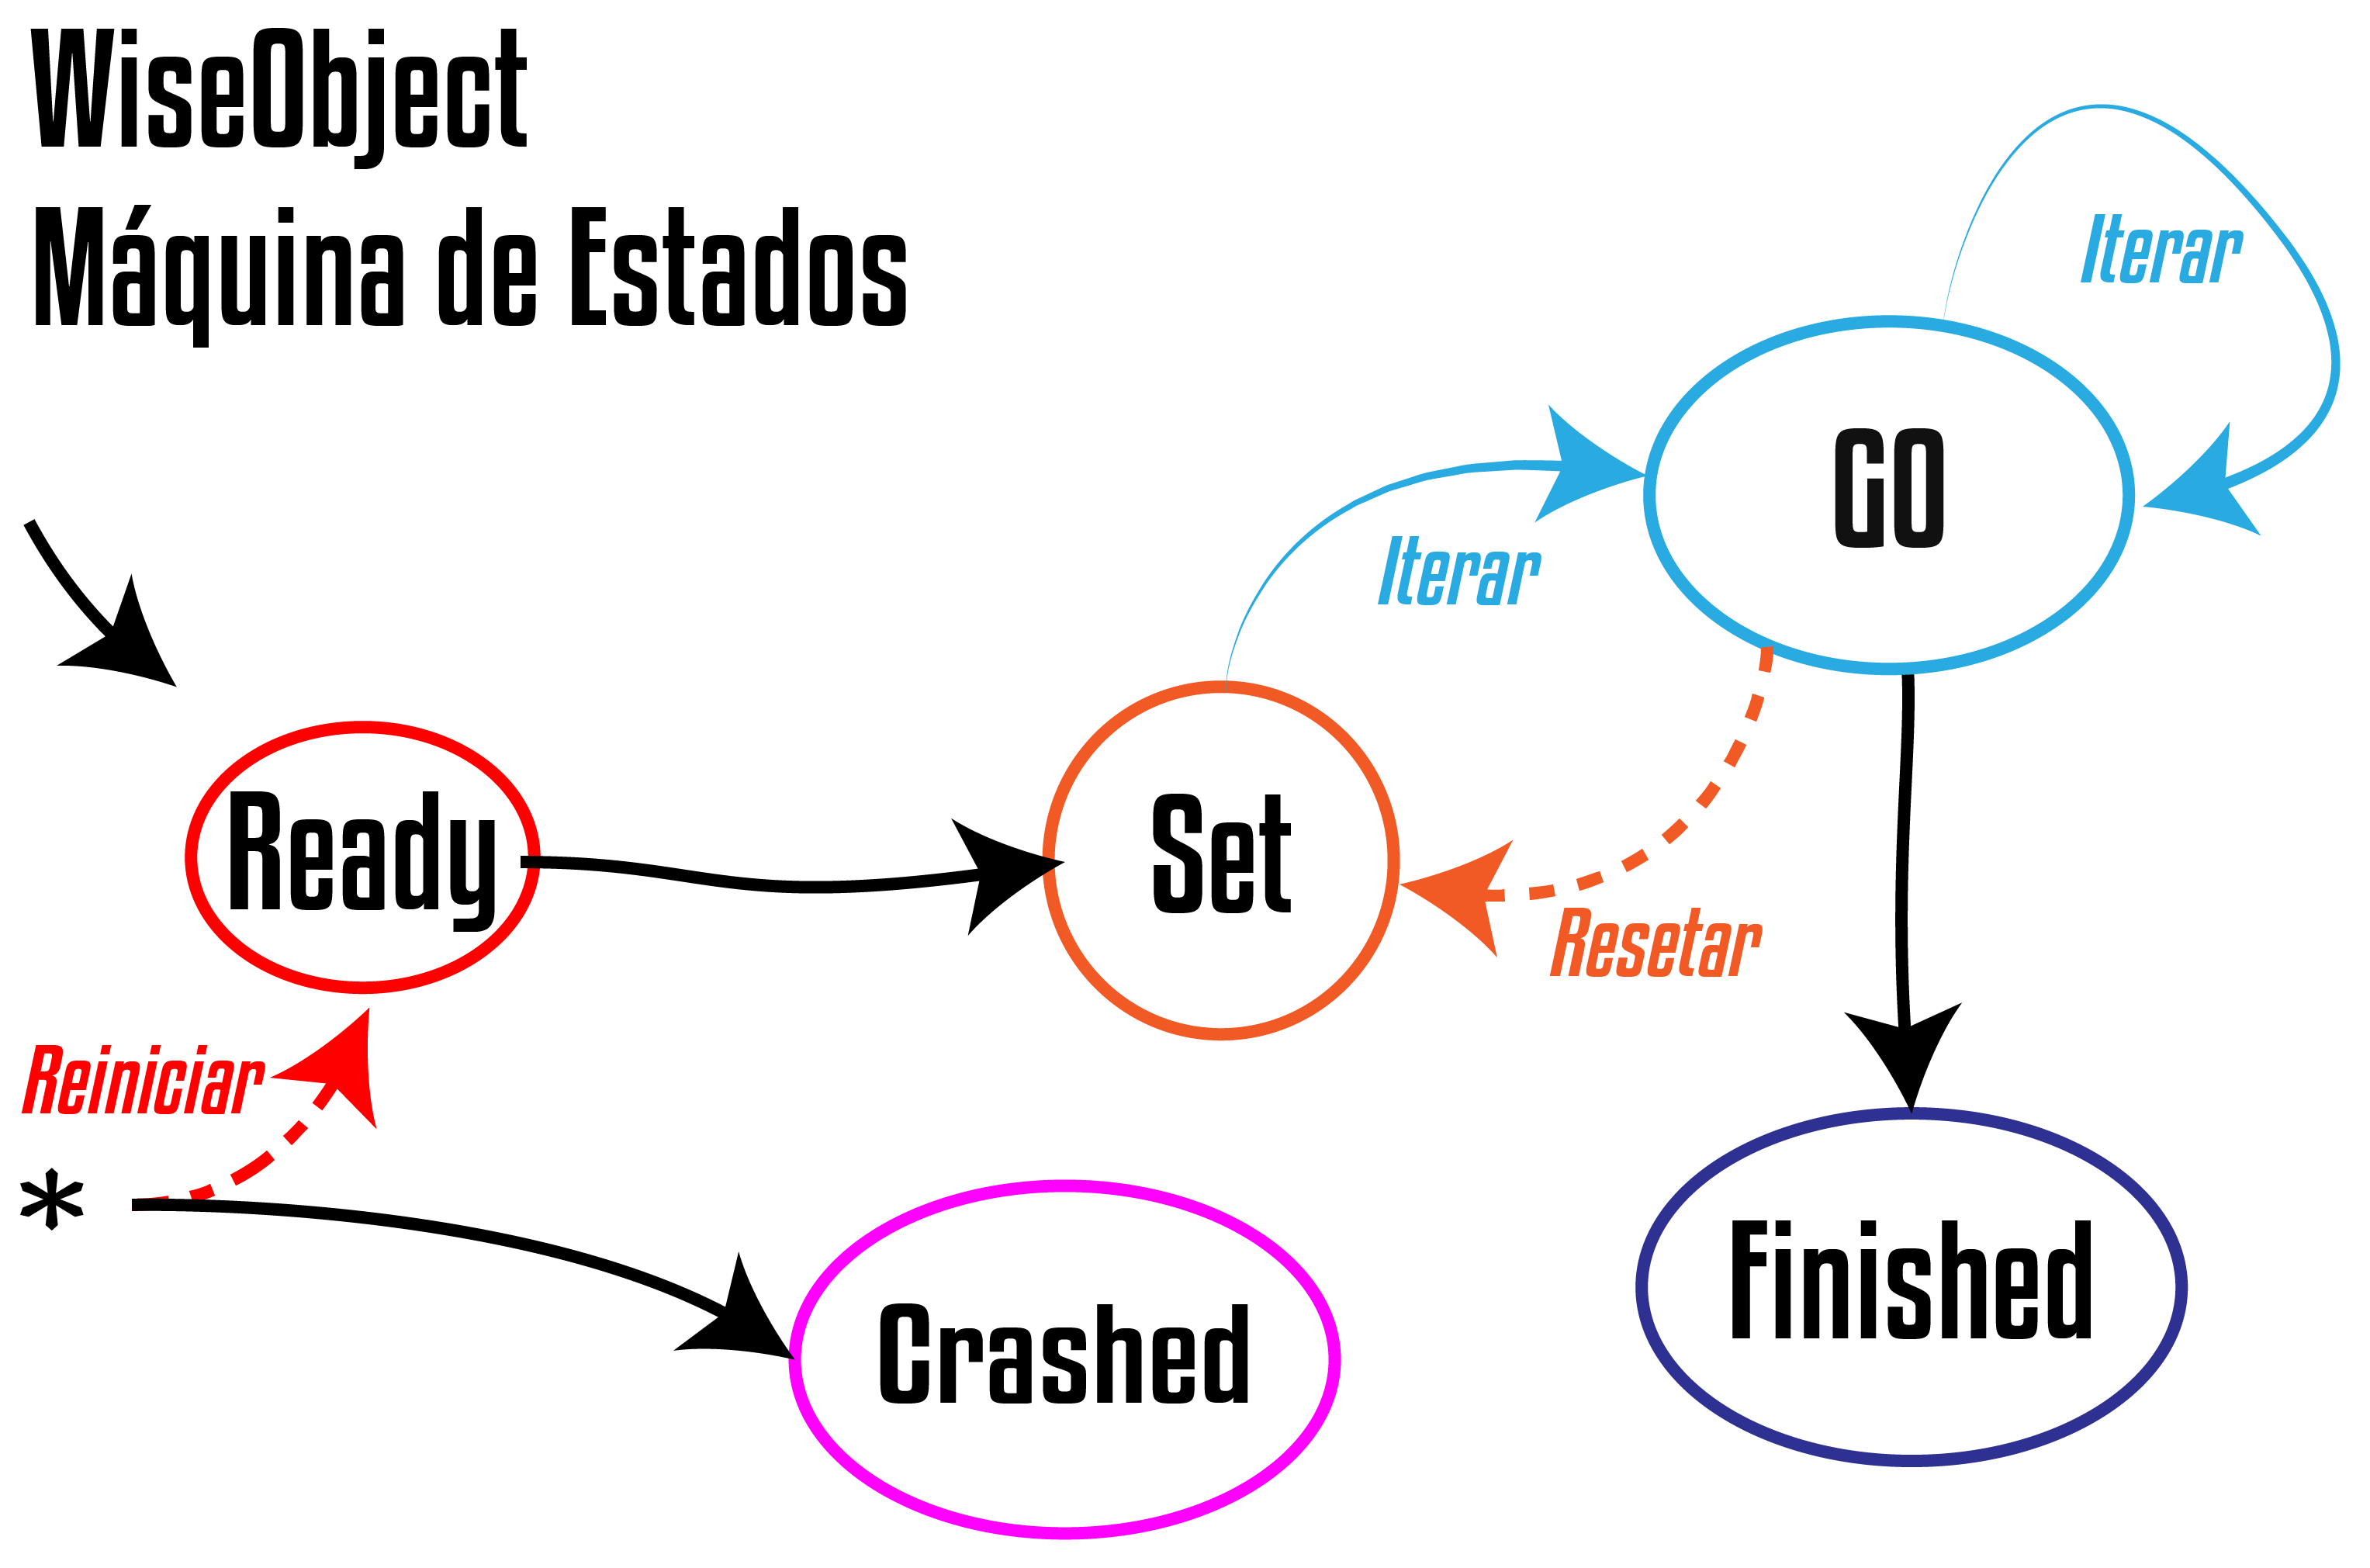
\includegraphics[scale=2]{Figures/WiseObjectStatus@16x.png}
	\caption{Máquina de estados utilizada pelos objetos inteligentes \textit{WiseObject}.}
	\label{fig7:wiseobjectstatuses}
\end{figure}

As trocas de estado dos objetos inteligentes são causadas por operações do usuário para preparar o objeto para iteração e para executar o método de iteração. Desta forma o usuário pode definir quais fábricas serão inseridas no objeto, parâmetros do modelo geométrico e do experimento e quais trocas de estados devem ser executadas.

Como objetos inteligentes são criados à partir de um elemento inteligente, eles possuem os mesmos métodos de criação. Desta forma, as fábricas de objetos inteligentes \textit{WiseObjectFactory} são compostas por fábricas de elementos inteligentes \textit{WiseElementFactory}. Finalmente, com este modelo de classes duas formas de criar objetos inteligentes foram disponibilizadas, utilizando um elemento inteligente já existente ou os métodos de criação de elementos disponíveis na fábrica de elementos inteligentes.

Em seguida é necessário definir qual será a lógica de iteração do objeto, adicionando uma fábrica de iteração \textit{WiseIterationFactory} compatível. Para o caso de escoamento pulsátil através de uma árvore arterial é necessário se adicionar a fábrica de iteração correspondente ao algoritmo da Seção~\ref{sec:algoritmo} e em seguida definir os parâmetros desejados, como a frequência $f$, a viscosidade $\mu$ e o ângulo de fase $\phi$. Com as alterações concluídas o objeto passa a poder ser iterado, opcionalmente uma fábrica gráfica \textit{GraphicFactory} pode ser inserida. Caso seja incluída, o objeto inteligente passará a gerar objetos gráficos \textit{GraphicObject} a cada iteração.

Inicialmente, um objeto é criado no estado \textit{Ready} com somente seu elemento inicial e uma fábrica do tipo \textit{WiseElementFactory}. Neste estado é esperada a inclusão das fábricas de iteração e gráficas. Uma vez que elas estejam corretamente acopladas ao objeto inteligente, é possível fazer a troca do estado \textit{Ready} para o estado \textit{Set}. Com a mudança de estado, é adicionado à estrutura inteligente \textit{WiseStructure} todos os parâmetros disponibilizados pelas fábricas de iteração e gráfica. Um objeto no estado \textit{Set} indica que o objeto foi corretamente criado, uma fábrica de iteração foi adicionada, possivelmente uma fábrica gráfica, e agora objeto aguarda alterações nestes parâmetros ou execução do método iterativo.

Com os parâmetros definidos e as fábricas devidamente acopladas os objeto está pronto para a iteração. O método iterativo de um objeto inteligente é representado na transição para o estado \textit{Go}. Uma iteração de uma \textit{WiseArteryTree} representa o cálculo dos valores de pressão e fluxo em toda a árvore arterial. Caso algum erro ocorra durante o processamento de dados o objeto se desloca para o estado \textit{Crashed}, assim como elementos inteligentes. É possível também finalizar a execução de um objeto inteligente o enviando para o estado \textit{Finished}, neste estado o objeto não poderá ser iterado novamente. Para que parâmetros da iteração possam ser alterados sem que se perda elementos inteligentes até então definidos, é possível que um objeto no estado \textit{Go} seja resetado e retorne para o estado \textit{Set}.

%--------------------------------------------------------------------------------%
\subsection{OBJETO GRÁFICO}\label{sec:objeto_grafico}


Quando o objeto inteligente \textit{WiseObject} estiver corretamente carregado e uma fábrica gráfica \textit{GraphicFactory} for adicionada à sua estrutura o primeiro objeto gráfico \textit{GraphicObject} de sua coleção será criado. Assim como o elemento inteligente representa uma iteração, um objeto gráfico representa um ciclo iterativo. Enquanto a estrutura responsável por elementos inteligentes, \textit{WiseCollection}, é responsável por manter os últimos dados de iteração aquecidos, a coleção de objetos gráficos \textit{GraphicModel} mantém o objeto que está sendo exibido por alguma tela e os mais próximos. As coleções tem como objetivo manter seus elementos e realizar trocas de estados quando necessário. No caso dos elementos inteligentes, somente o último objeto é necessário e isso não muda, no contexto dos objetos gráficos apenas o objeto exibido em um elemento da interface de usuário e seus vizinhos serão mantidos em memória.

\begin{figure}[!htbp]
	\centering
	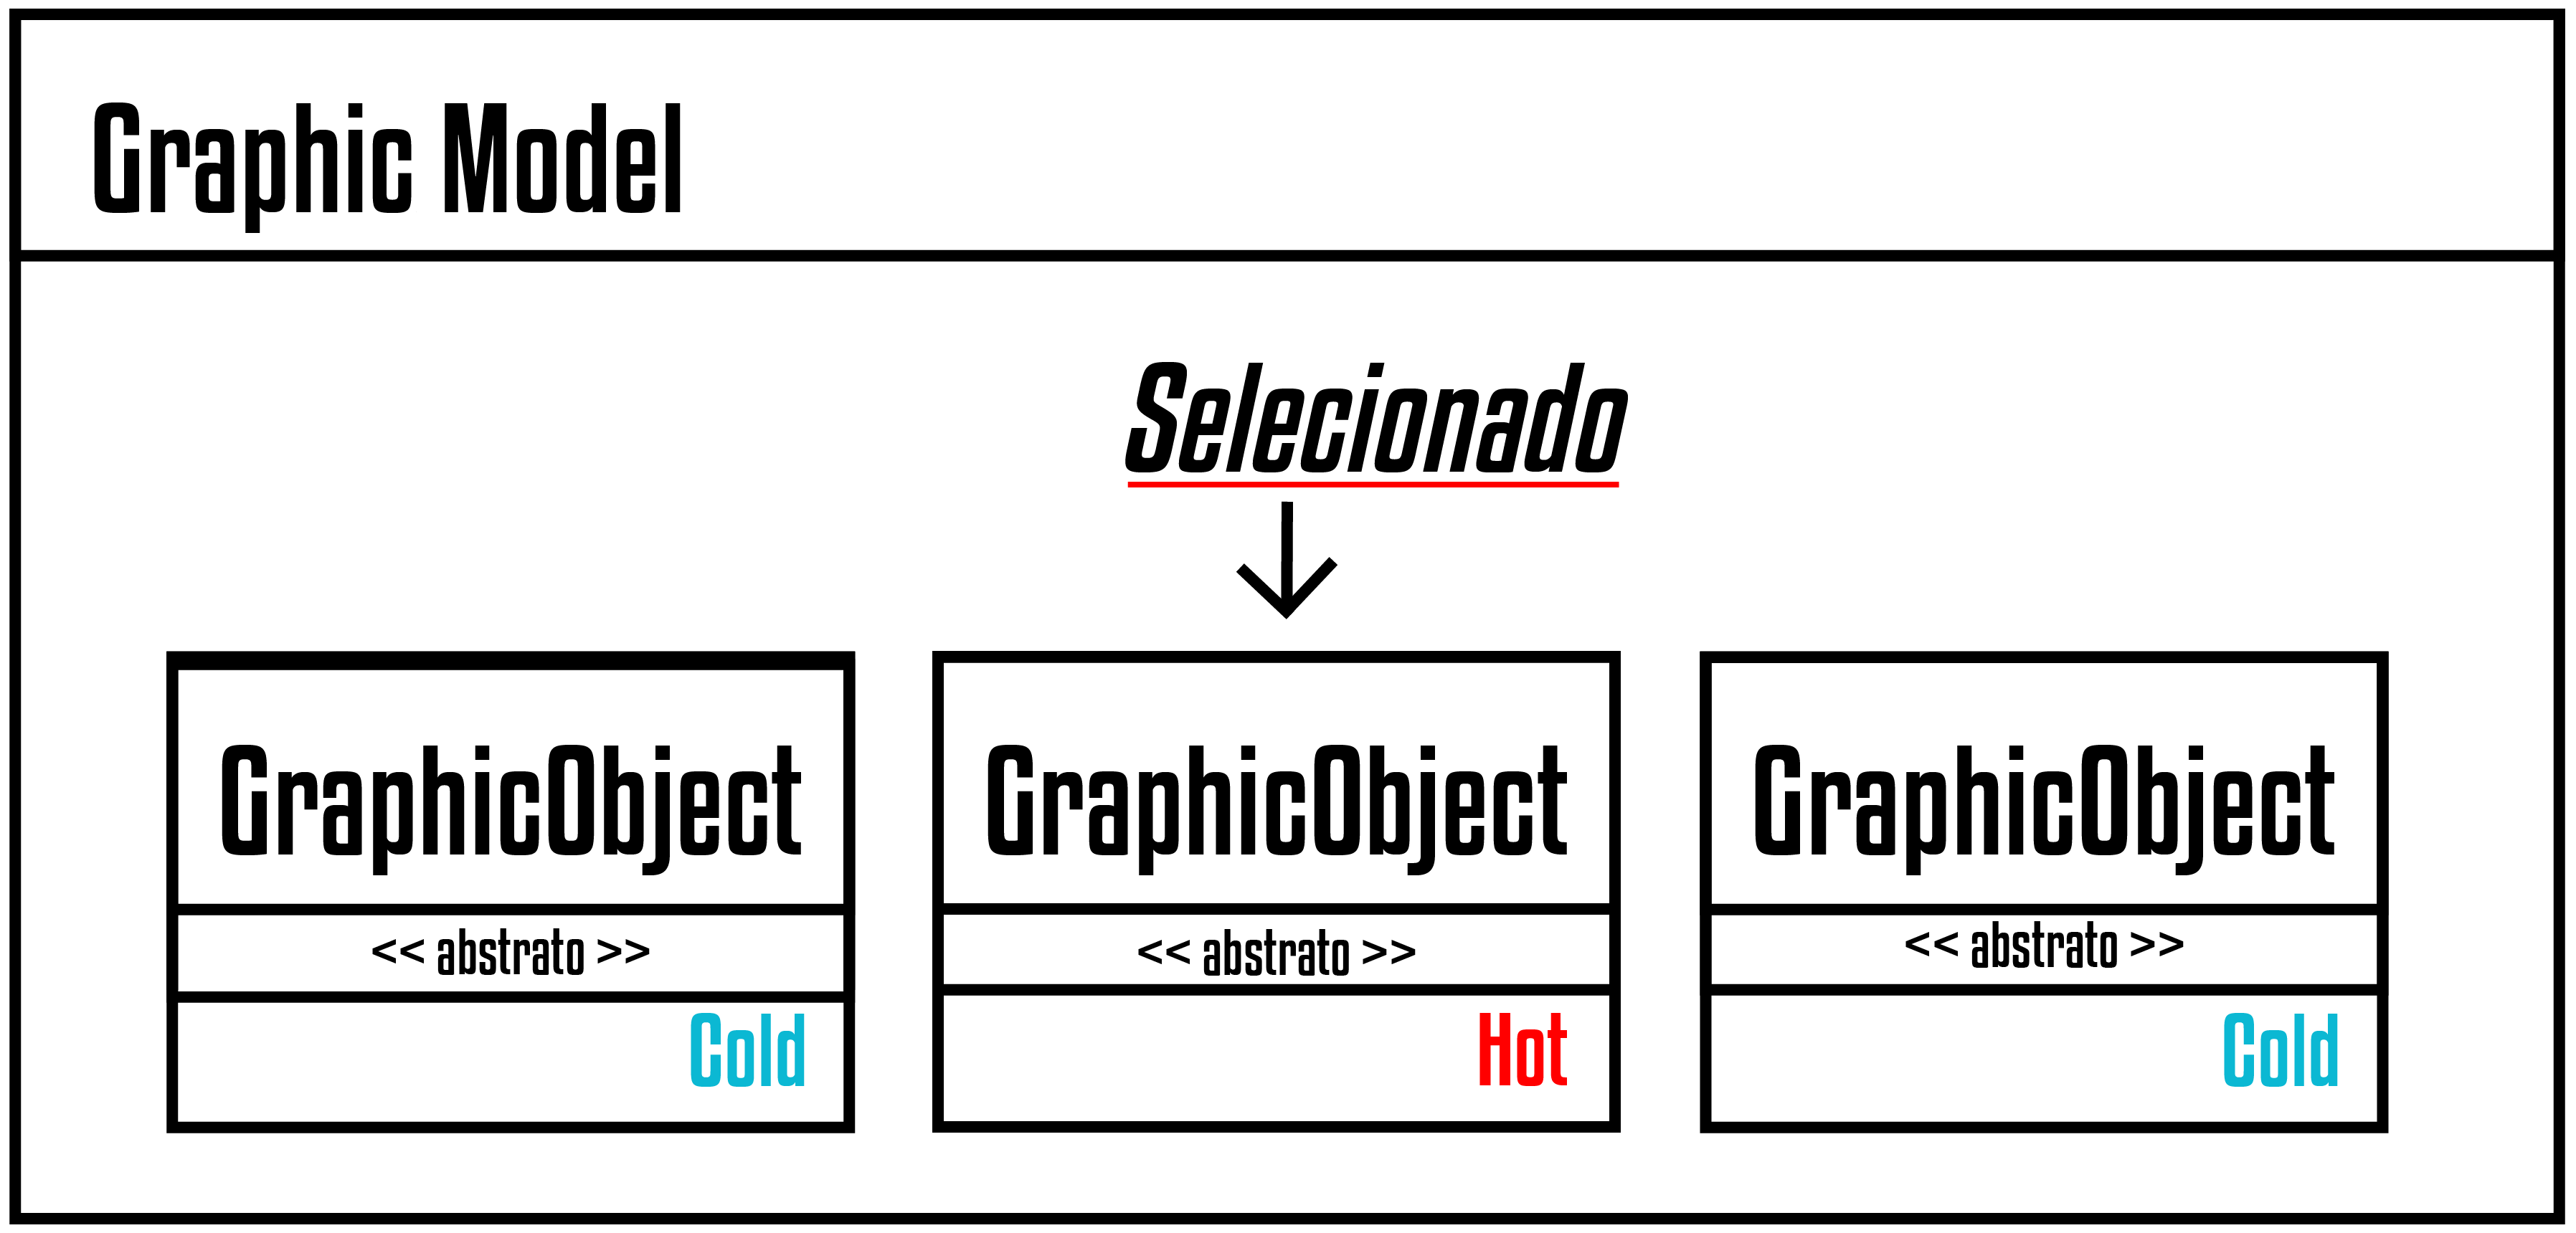
\includegraphics[scale=2]{Figures/GraphicModel@16x.png}
	\caption{Modelo gráfico \textit{GraphicModel}, contém uma coleção de objetos gráficos.}
	\label{fig7:graphicmodel}
\end{figure}

Presente na Figura~\ref{fig7:graphicmodel} estão os componentes que permitem armazenar todos os quadros da animação final. Quando um objeto \textit{WiseObject} está corretamente configurado com uma instância de fábrica gráfica \textit{GraphicFactory}, seu método iterativo é atrelado à criação de objetos gráficos. Isso permite que o objeto iterado crie um elemento inteligente \textit{WiseElement} e um objeto gráfico \textit{GraphicObject} à cada iteração.

\begin{figure}[!htbp]
	\centering
	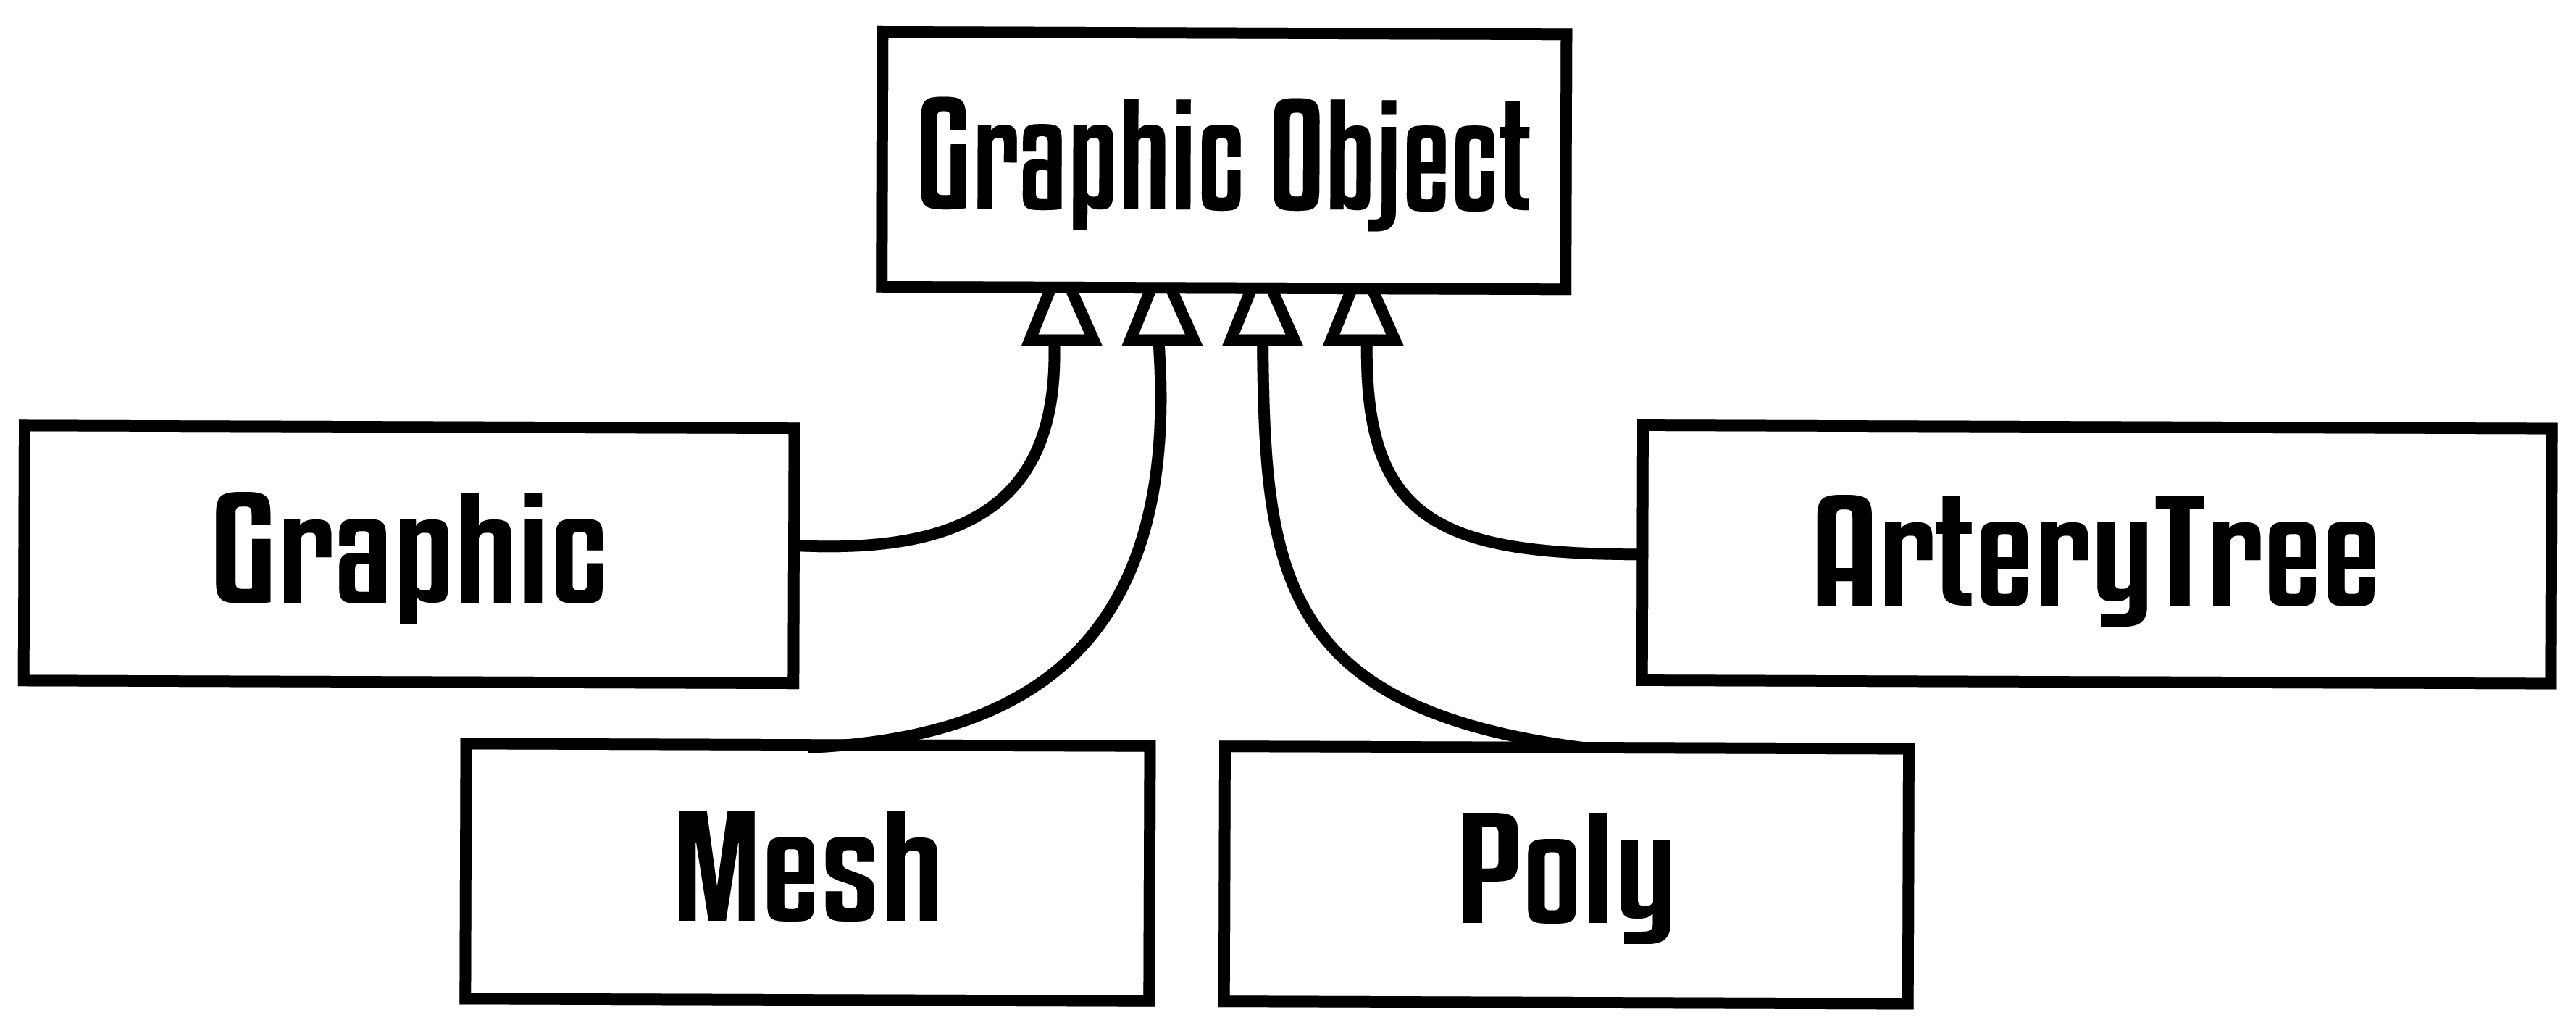
\includegraphics[scale=2]{Figures/GraphicObjects@16x.png}
	\caption{Tipos de objetos gráficos \textit{GraphicObjects}.}
	\label{fig7:graphicobjects}
\end{figure}

Cada objeto gráfico se desenha através de diretivas OpenGL, o formato do modelo geométrico é apresentado ao usuário através das formas desenhadas, enquanto algum parâmetro do elemento inteligente \textit{WiseElement} é visualizado através de uma escala de cores.

Os objetos gráficos contidos na Figura~\ref{fig7:graphicobjects} possuem métodos específicos para se desenhar utilizando um gradiente de cores e formas geométricas padrão, bidimensionais ou tridimensionais. Cada forma geométrica utilizada é representada por elementos gráficos \textit{GraphicElement}. A cada iteração  a fabrica utilizará o elemento inteligente contido na estrutura \textit{Forno}, retirando a informação do elemento inteligente mais atual. Cada objeto gráfico possui um valor máximo e mínimo que é vinculado ao gradiente cores, com isso as cores representam os valores armazenados em cada objeto gráfico.

\begin{figure}[!htbp]
	\centering
	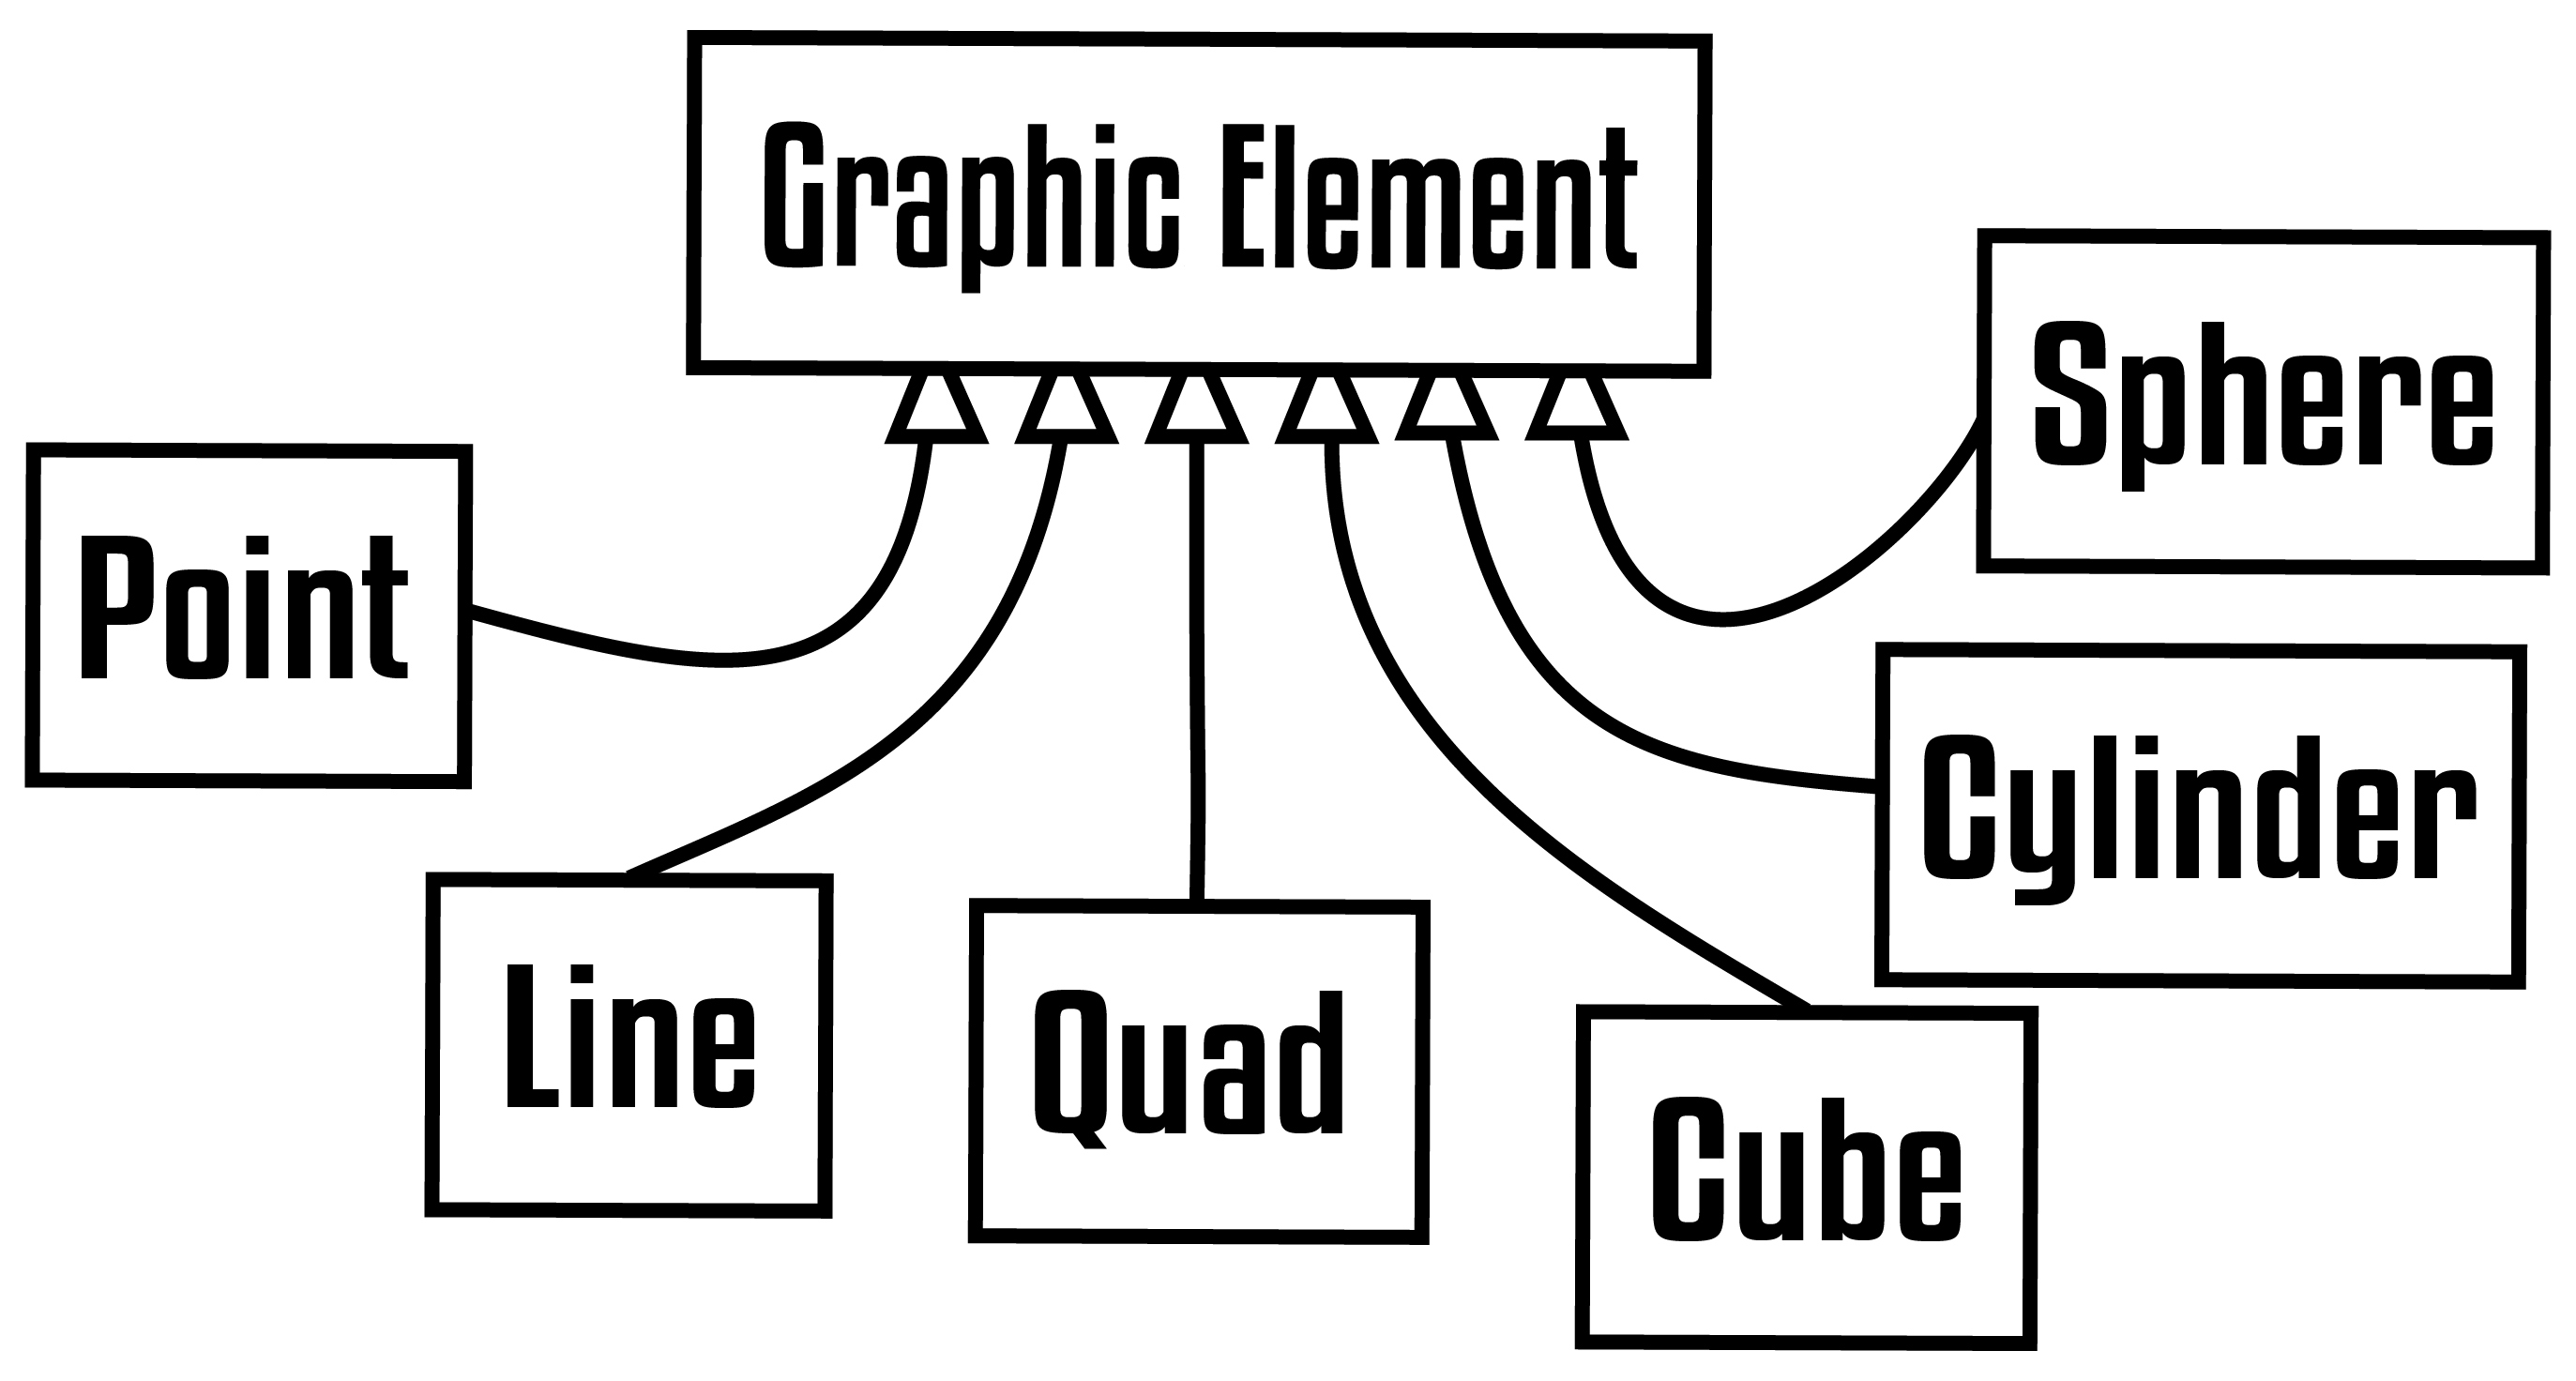
\includegraphics[scale=2]{Figures/GraphicElements@16x.png}
	\caption{Tipos de elementos gráficos \textit{GraphicElements}. \textit{Point}, um ponto. \textit{Line}, uma linha. \textit{Quad}, um quadrado. \textit{Cube}, um cubo. \textit{Cylinder}, um cilindro. \textit{Sphere}, uma esfera.}
	\label{fig7:graphicelements}
\end{figure}

Os elementos gráficos podem ser utilizados por qualquer tipo de objeto gráfico. A representação geométrica de uma árvore arterial é construída utilizando cilindros e esferas, que representam segmentos de vaso e terminais, respectivamente. Por padrão, os cilindros receberão uma lista de valores da pressão $P(X) \forall X \in [0,1]$, enquanto as esferas receberão os valores da pressão $P(X)$ quando $X=0$ ou $X=1$, condicionado a escolha do nó distal($X=1$) ou o nó proximal($X=0$).  Assim como os objetos inteligentes \textit{WiseObject} têm seus tipos definidos pelo tipo de elemento inteligente que o compõe, o objeto gráfico \textit{GraphicObject} tem seu tipo definido pelo elemento inteligente que representa, com sua fábrica própria.

Apesar do objeto gráfico \textit{GraphicObject} ser uma redundância dos dados armazenados em um elemento inteligente \textit{WiseElement}, ele é menor, podendo ser carregado e armazenado mais rapidamente. O objetivo das estruturas nesta seção é permitir que diversos objetos gráficos \textit{GraphicObjects} possam ser armazenados  e rapidamente carregados em memória. Os objetos gráficos em sequência representam uma animação que pode ser visualizada através da interface gráfica. 


%--------------------------------------------------------------------------------%
\subsection{PROJETO INTELIGENTE}\label{sec:projeto}

Os projetos inteligentes \textit{WiseProject} são os escopos de trabalho da ferramenta computacional, sendo utilizada na organização dos objetos dentro da ferramenta computacional. O primeiro passo para se utilizar a ferramenta é criar um projeto inteligente que irá conter todos os objetos e elementos inteligentes criados.


\begin{figure}[!htbp]
	\centering
	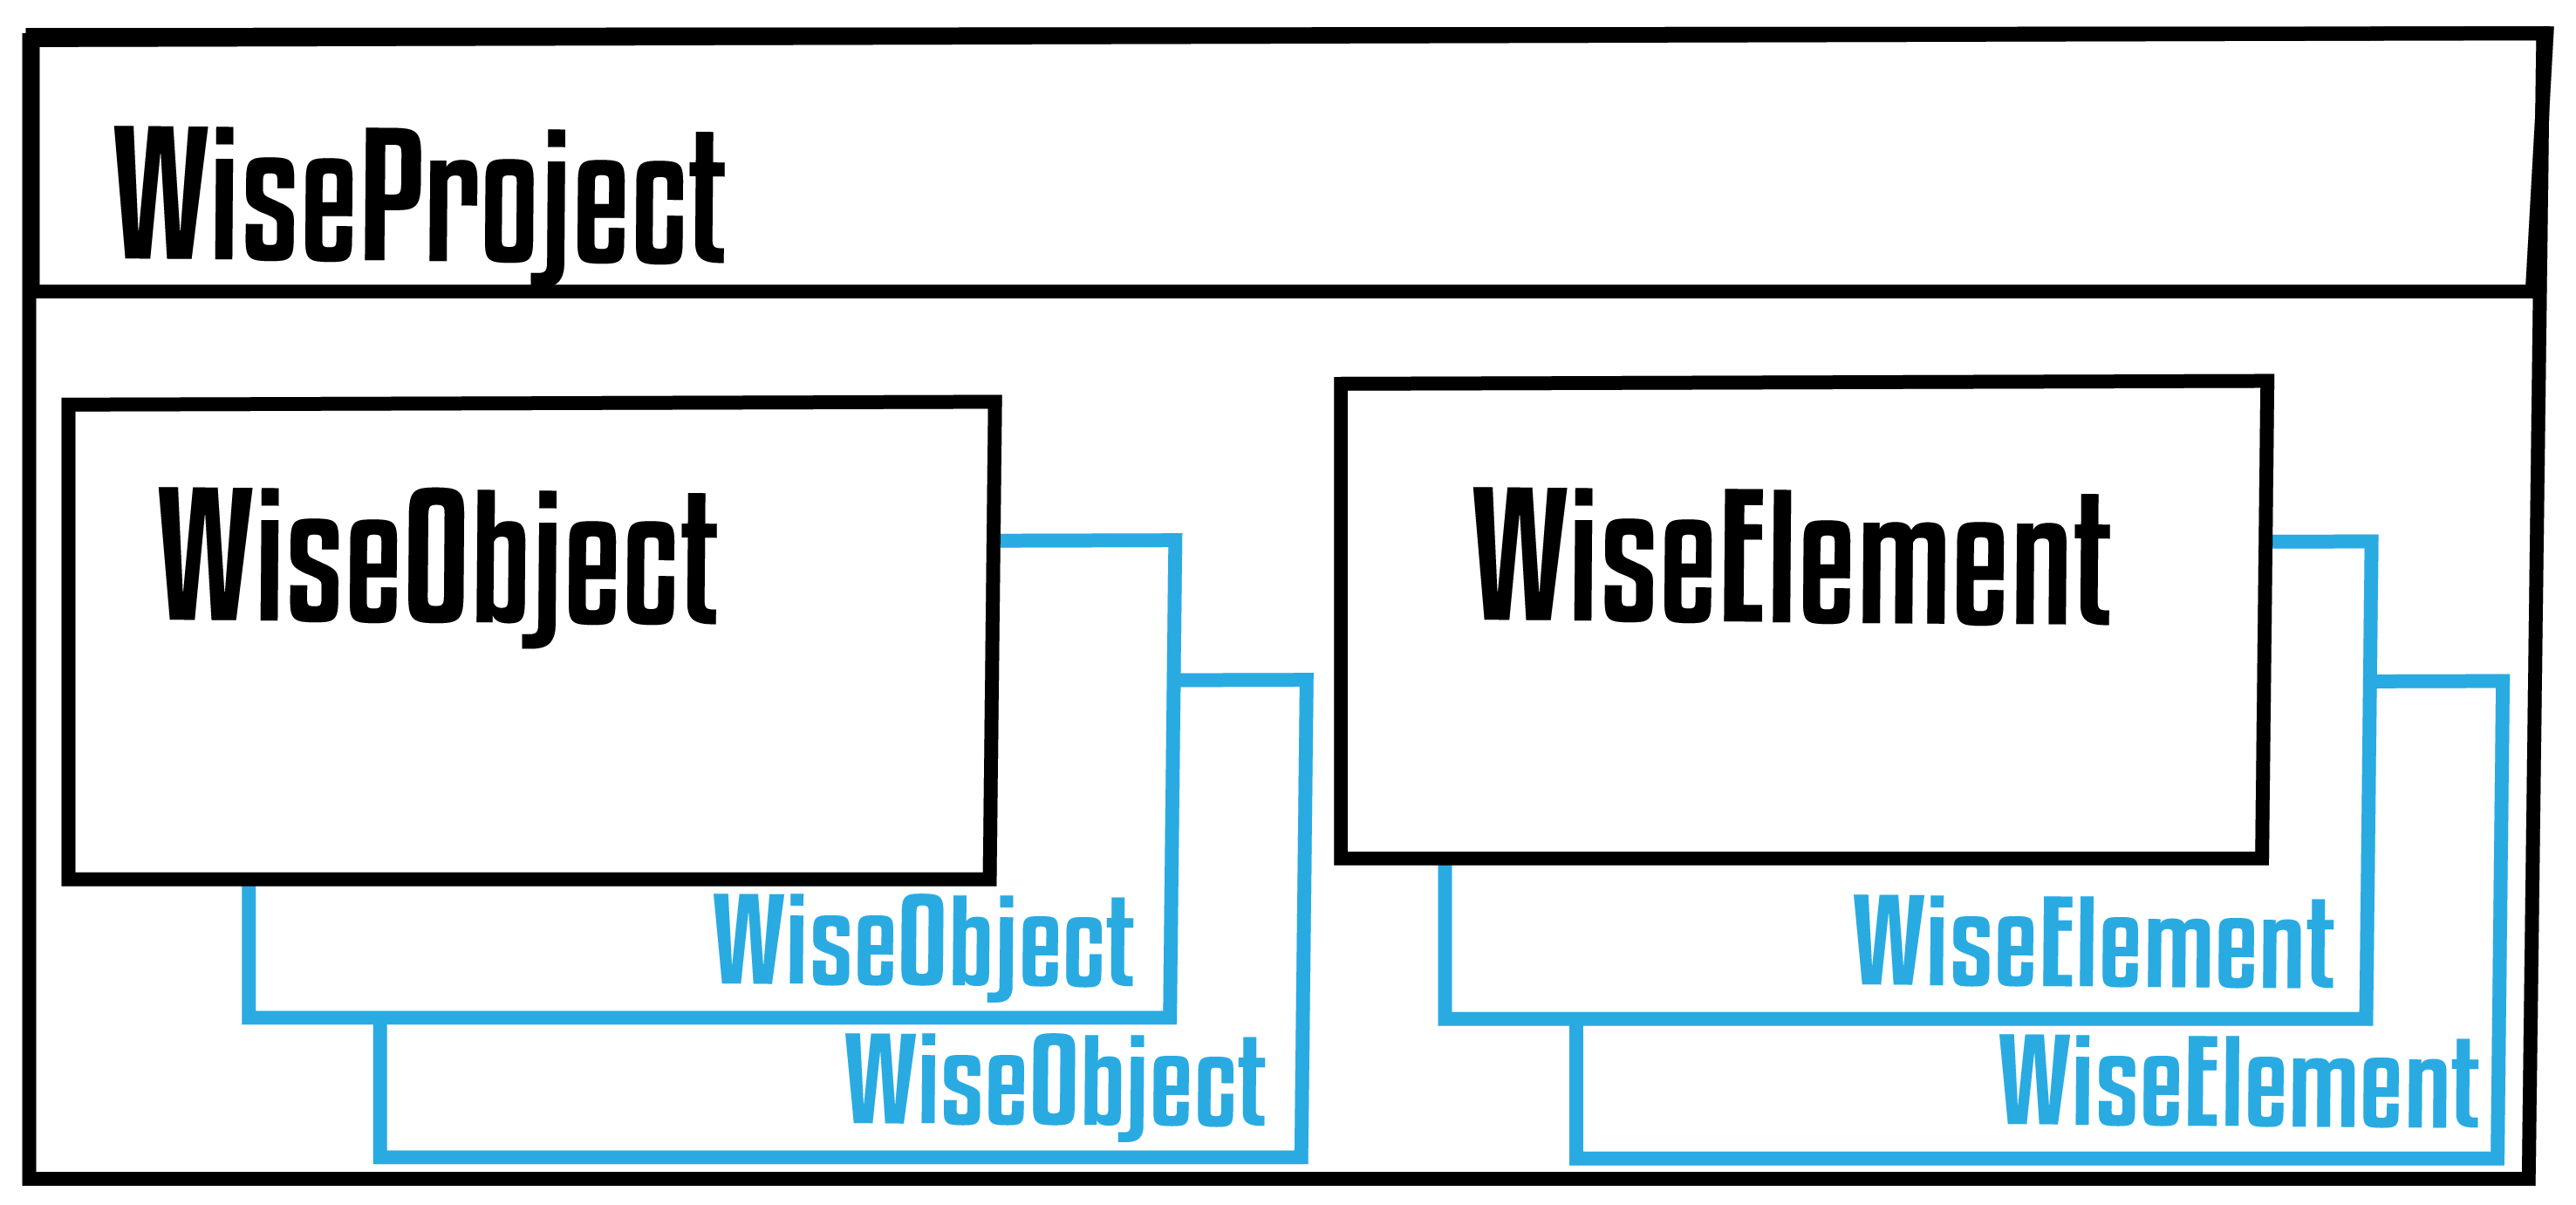
\includegraphics[scale=2]{Figures/WiseProject@16x.png}
	\caption{Projeto inteligente \textit{WiseProject} e seus componentes, uma lista de objetos inteligentes \textit{WiseObject} e uma lista de elementos inteligentes \textit{WiseElement}.}
	\label{fig7:project}
\end{figure}

Como demonstrado na Figura~\ref{fig7:project}, os projetos inteligentes são representados por duas coleções, uma de elementos inteligentes \textit{WiseElement} e outra de objetos inteligentes \textit{WiseObject}. Os comandos recebidos pela ferramenta computacional terão efeito apenas sobre um projeto inteligente e suas coleções. Por exemplo, quando um elemento inteligente for utilizado na criação de um objeto inteligente eles devem estar no mesmo projeto inteligente.

Os projetos inteligentes são estrutura organizacionais, uma vez que um comando é executado sobre objetos de um projeto, esses objetos são bloqueados pelo projeto. Ao excluir um projeto, todas as demandas devem ser finalizadas. Finalmente, as estruturas dos projetos podem ser salvas e carregadas, portanto estas estruturas servem também para armazenar experimentos inteiros e seus resultados.

%--------------------------------------------------------------------------------%
\subsection{FÁBRICA DE PROJETO}\label{sec:fabrica_projeto} 

O conceito de fábrica foi adicionado ao projeto para padronizar a construção de objetos, inclusa neste conceito, a fábrica de projetos \textit{WiseProjectFactory} é responsável pela construção de projetos. Diferentemente das outras fábricas, a fábrica de projetos inteligentes contém todas as fábricas suportadas pela ferramenta computacional.

\begin{figure}[!htbp]
	\centering
	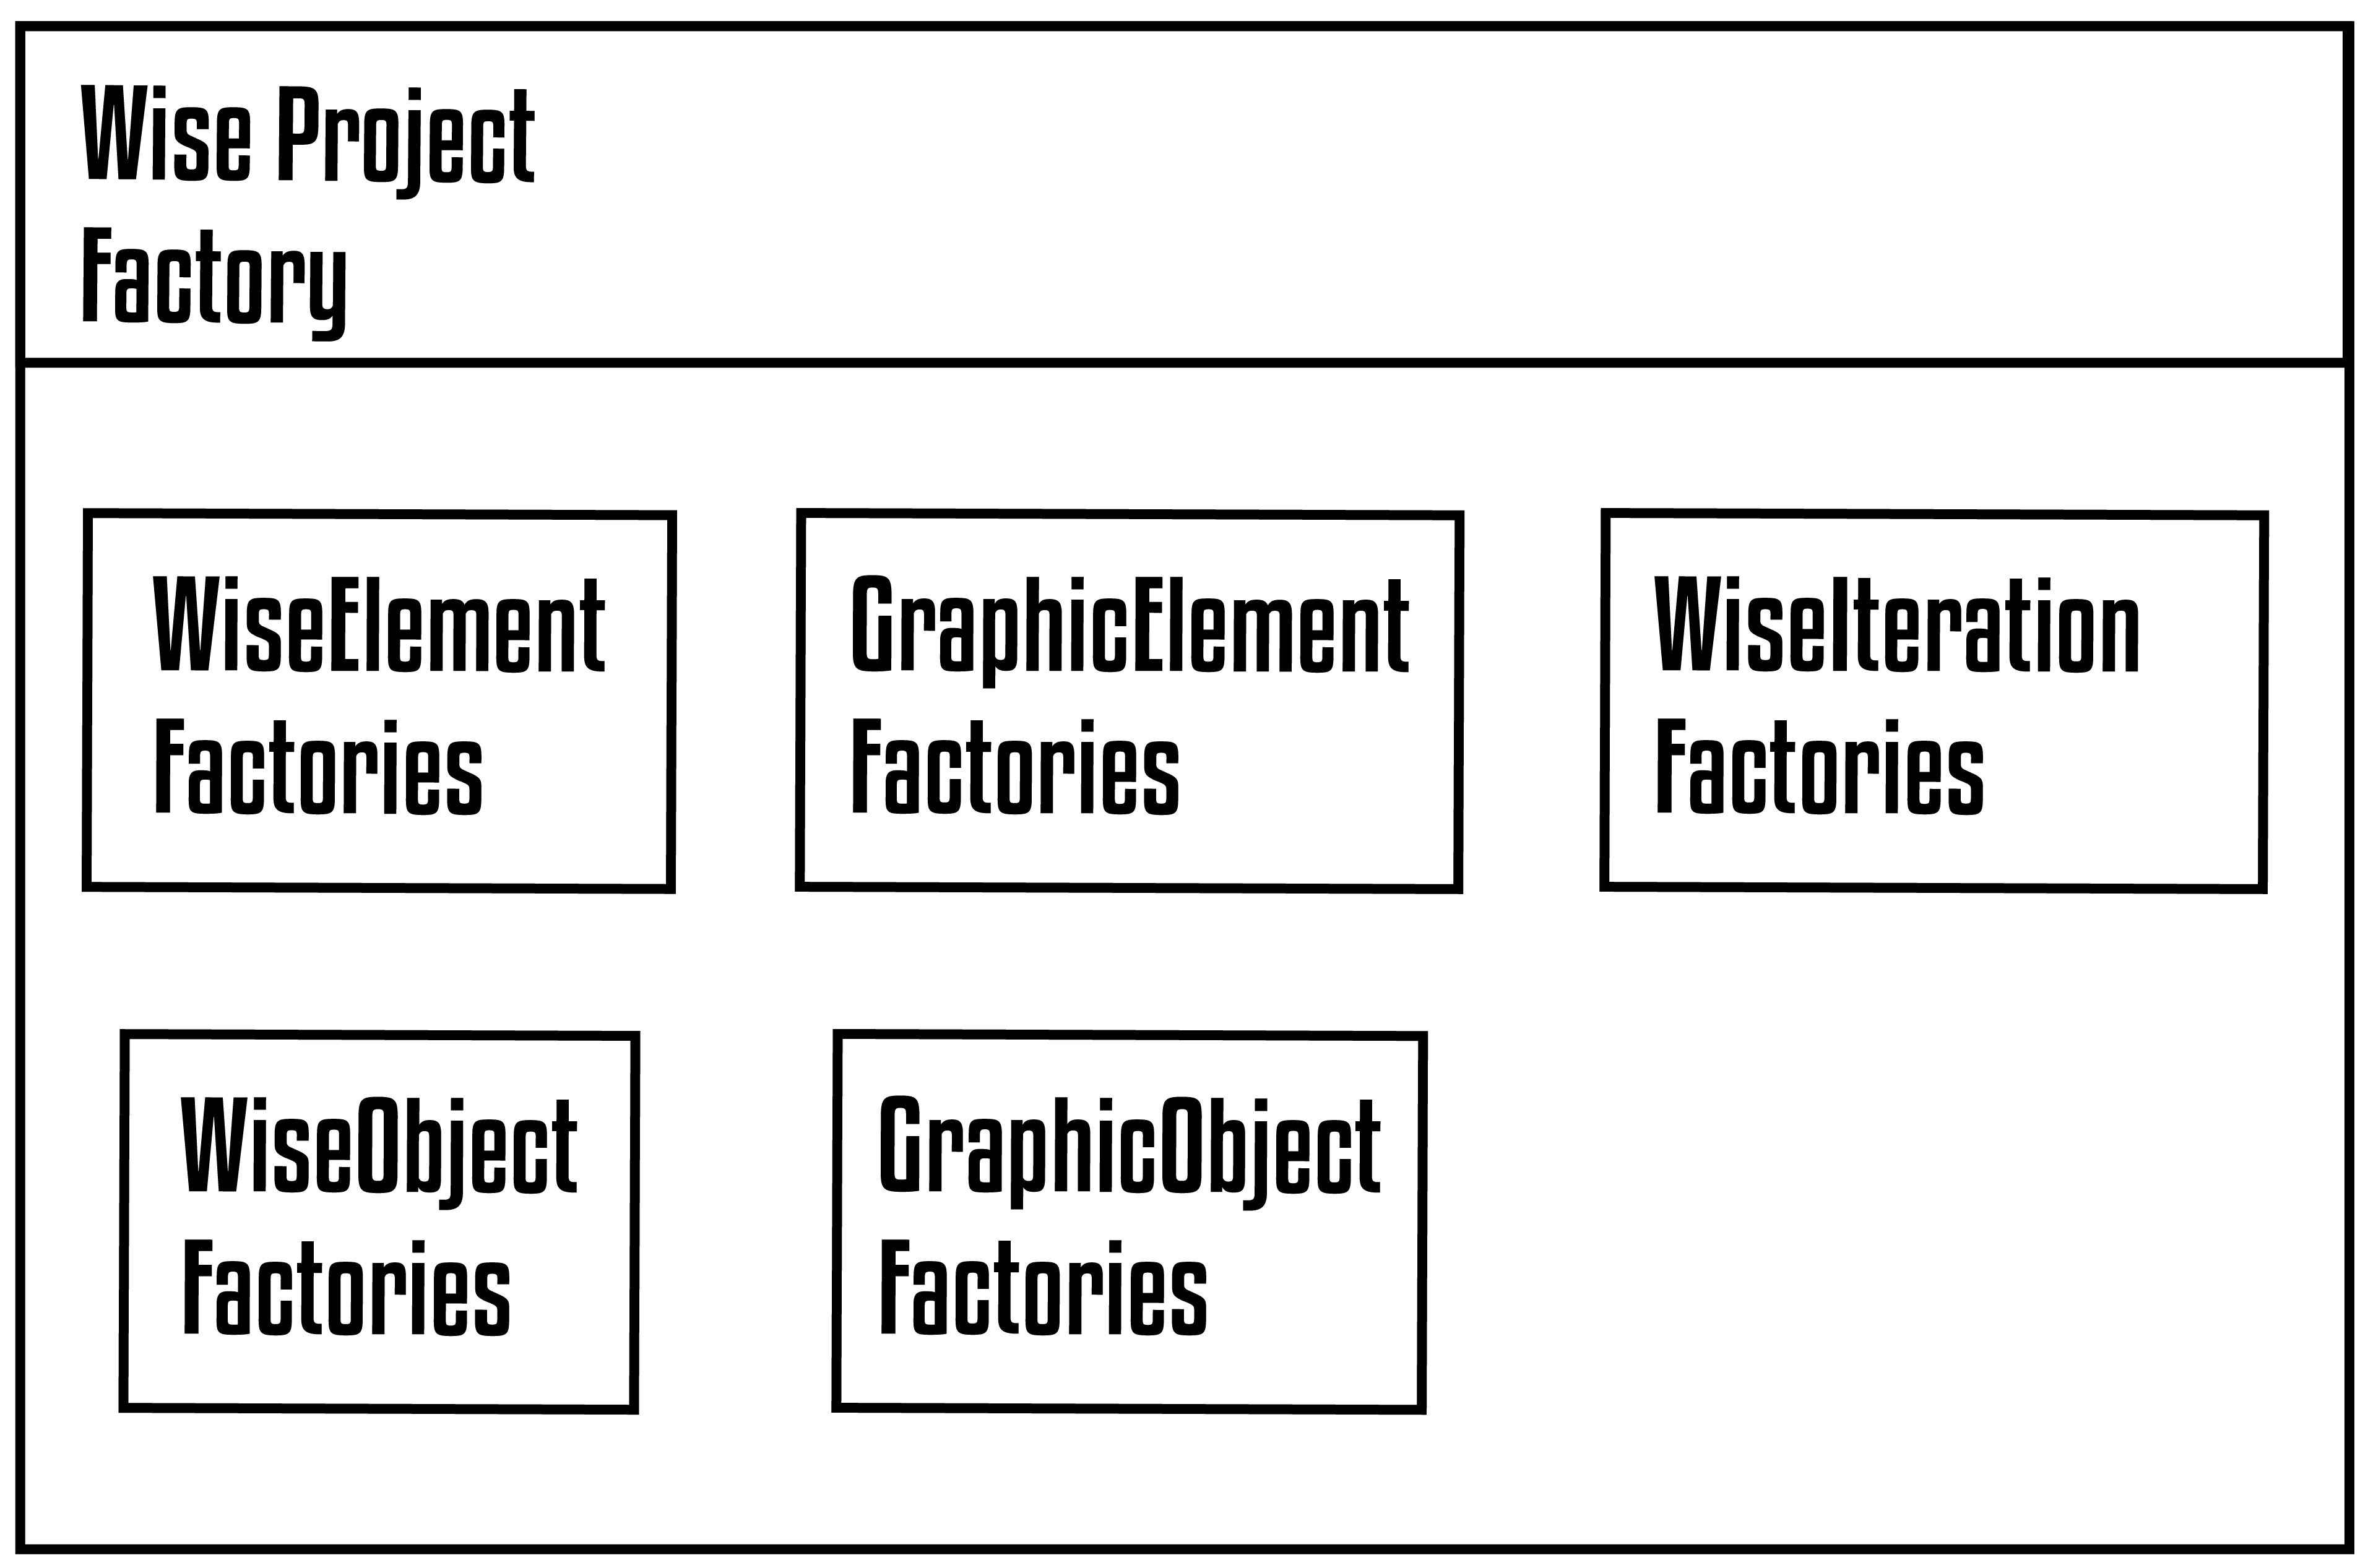
\includegraphics[scale=1.5]{Figures/WiseProjectFactory@16x.png}
	\caption{Fábrica de projetos inteligentes \textit{WiseProjectFactory} e seus componentes, fábricas de elementos inteligentes \textit{WiseElementFactories}, fábricas de objetos inteligentes \textit{WiseObjectFactories}, fábrica de objetos gráficos \textit{GraphicObjectFactories}, fábricas de elementos gráficos \textit{GraphicElementFactories} e fábricas de iteração \textit{WiseIterationFactories} .}
	\label{fig7:projectfactory}
\end{figure}

Como é possível observa na Figura~\ref{fig7:projectfactory}, a fábrica de projetos inteligentes é composta de outras coleções de fábricas, agrupadas pelo tipo de estrutura que criam. Nesta classe estão as fábricas de elementos inteligentes \textit{WiseElement}, objetos inteligentes \textit{WiseObject}, objetos gráficos \textit{GraphicObject}, elementos gráficos \textit{GraphicElement} e iteração \textit{WiseIterationFactory}. Por exemplo, quando um projeto contendo diversas árvores arteriais e gráficos é carregado ele é construído pela fábrica de projetos. A fábrica de projetos irá reconhecer o formato de cada estrutura e encaminhar para a fábrica correspondente.

\begin{figure}
	\begin{tabular}{cc}
		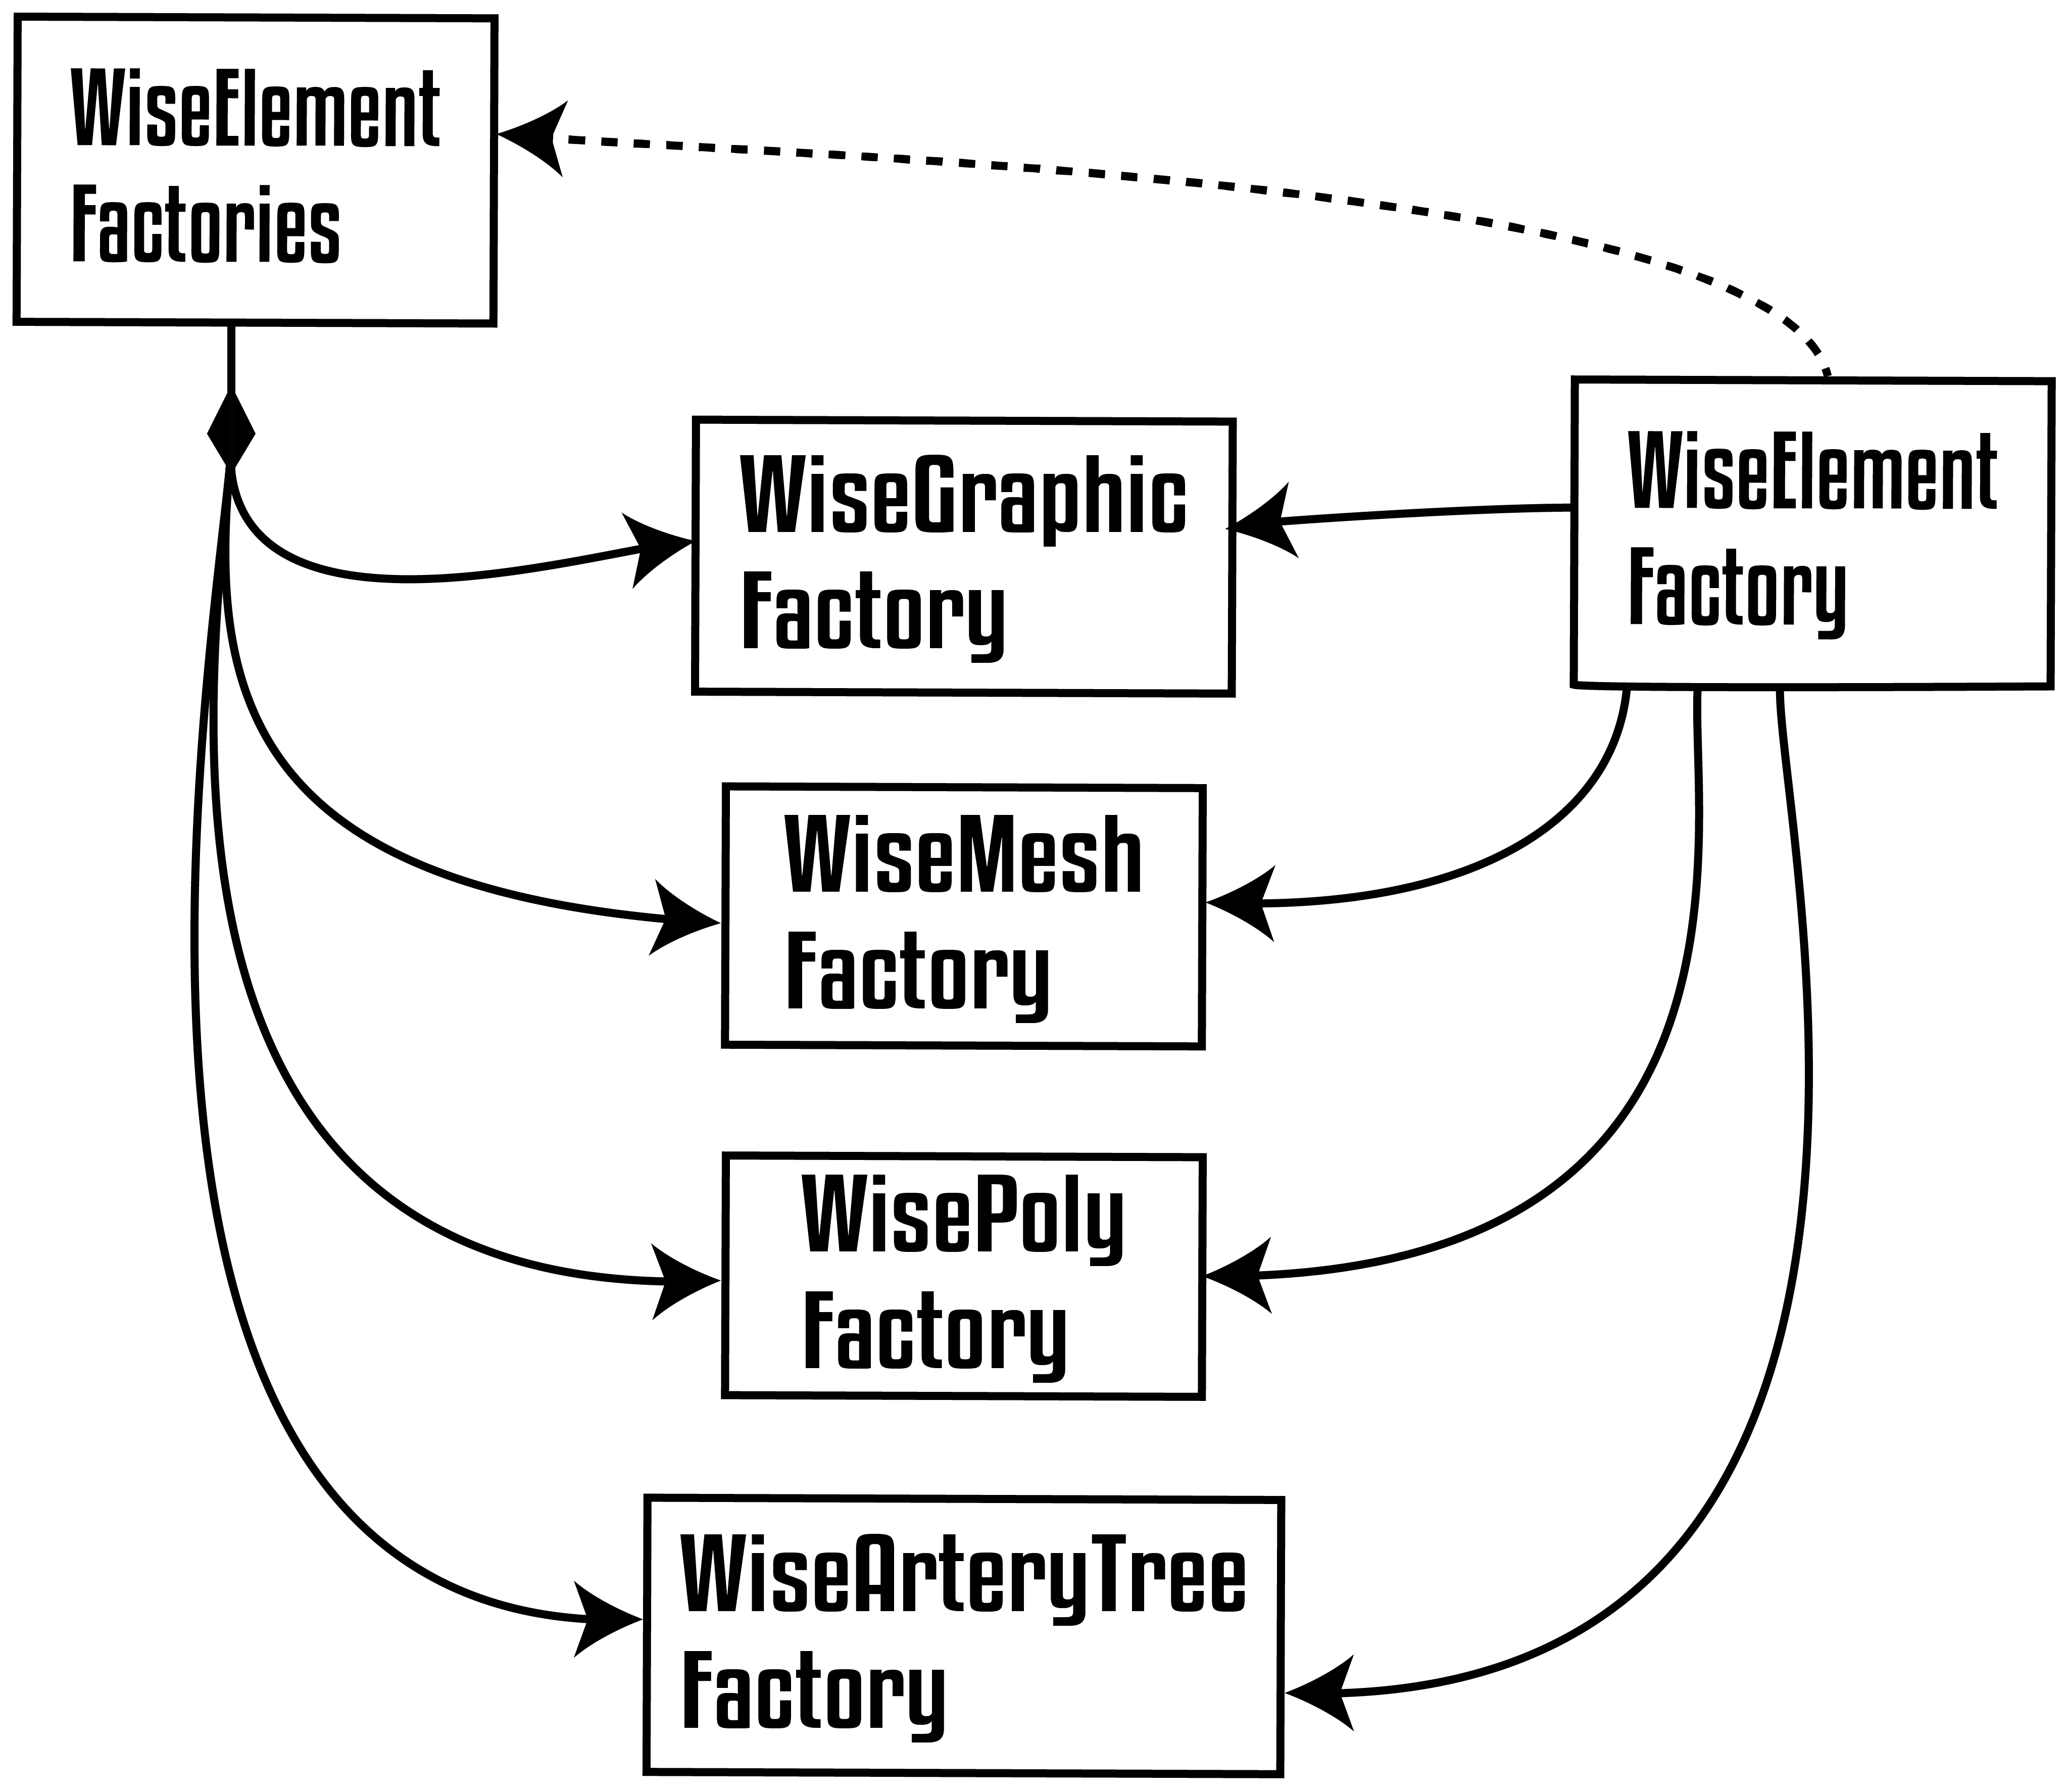
\includegraphics[width=0.5\linewidth]{Figures/WiseElementFactories@16x.png} &   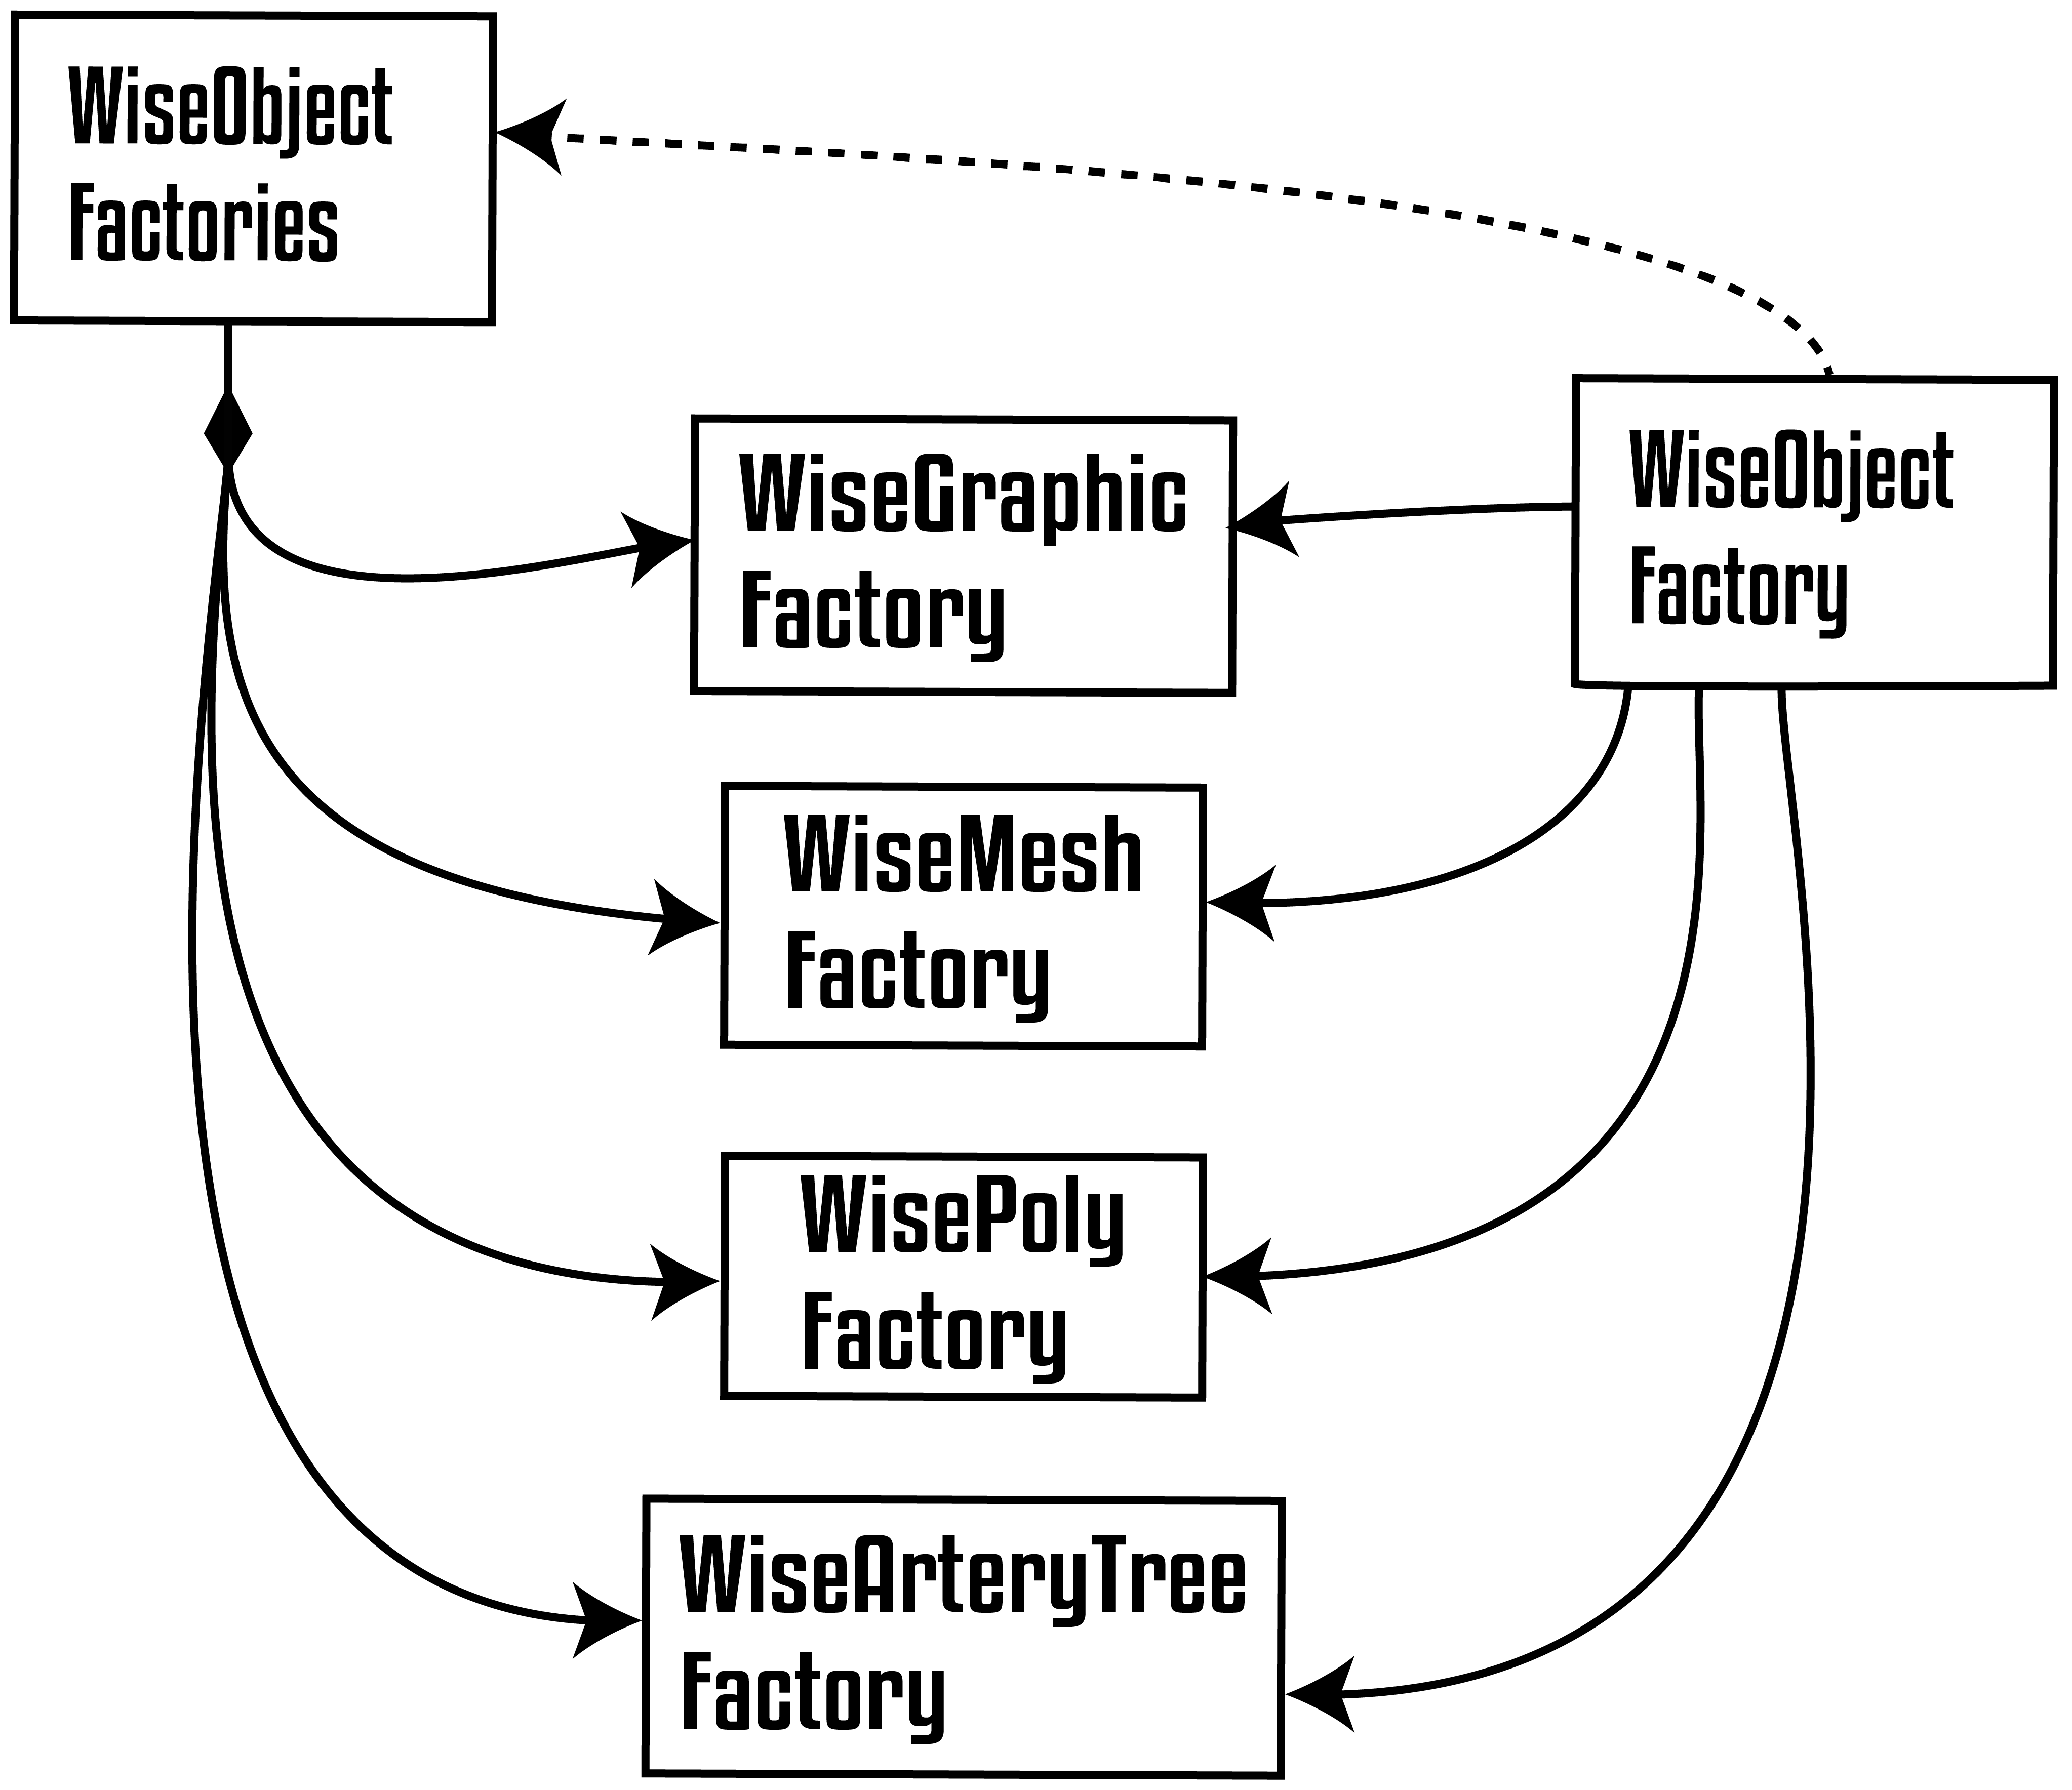
\includegraphics[width=0.5\linewidth]{Figures/WiseObjectFactories@16x.png} \\
		(a) Fábricas de elementos inteligentes & (b) Fábricas de objetos inteligentes \\[6pt]
		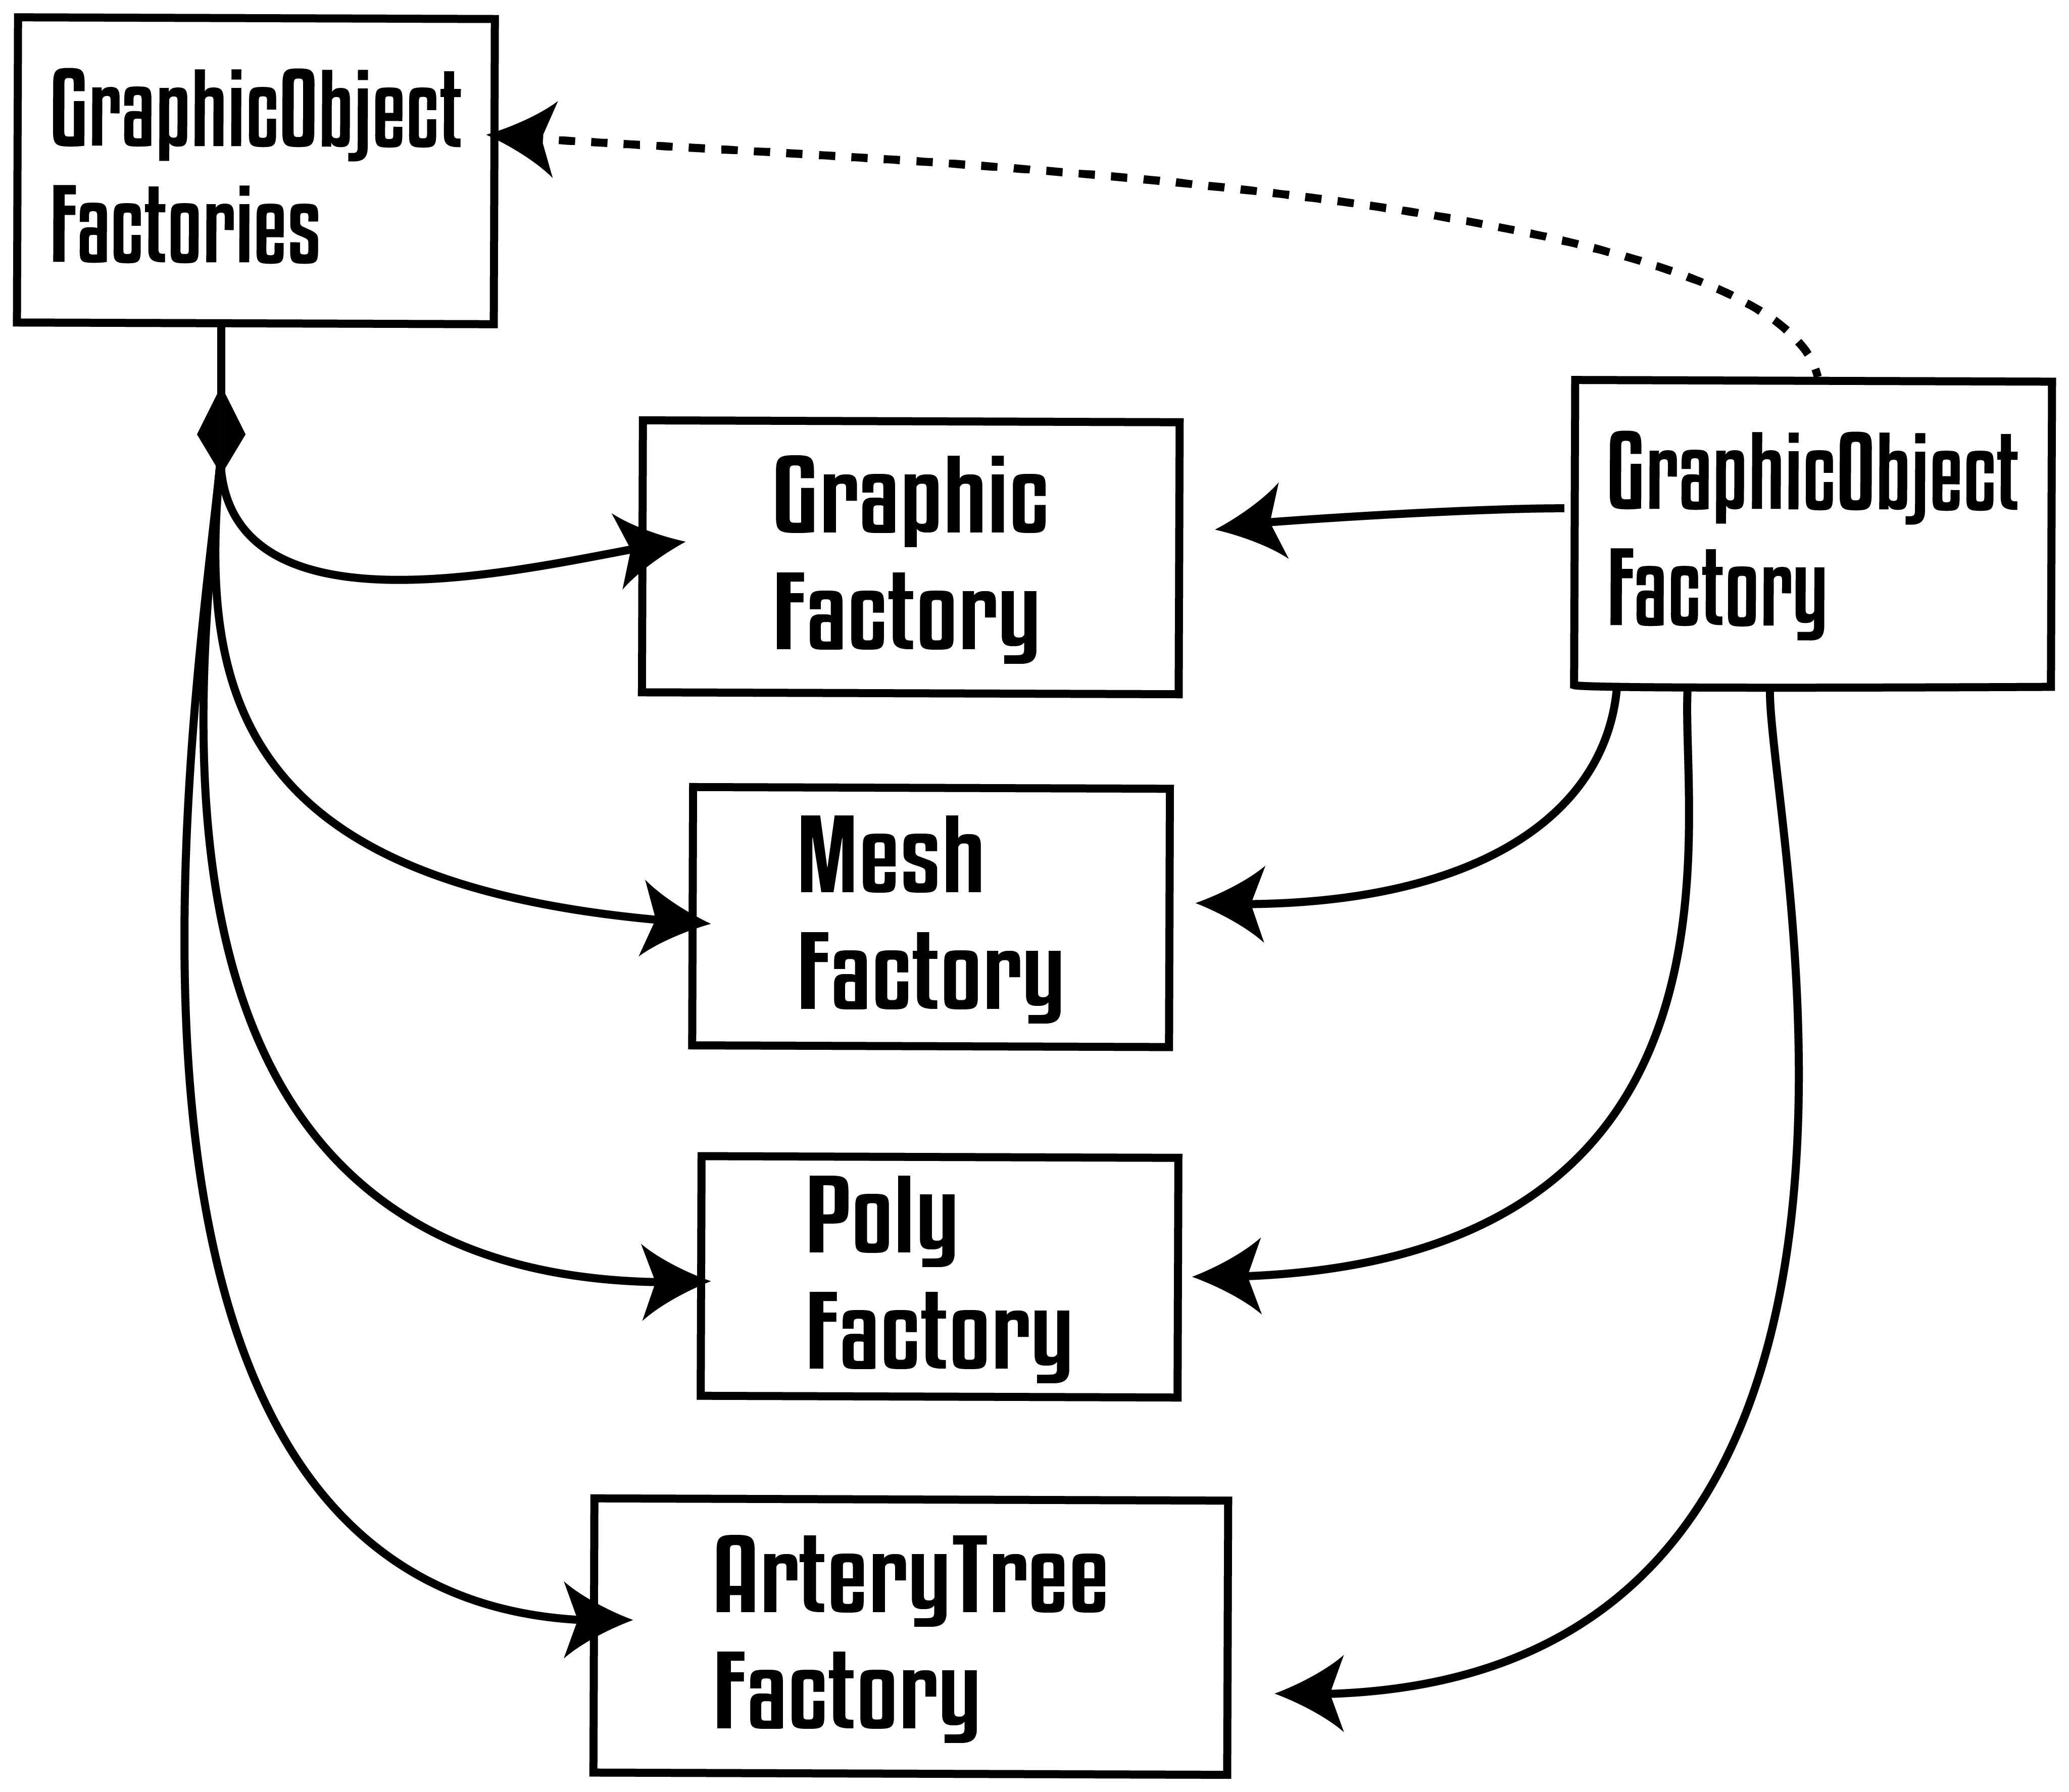
\includegraphics[width=0.5\linewidth]{Figures/GraphicObjectFactories@16x.png} &   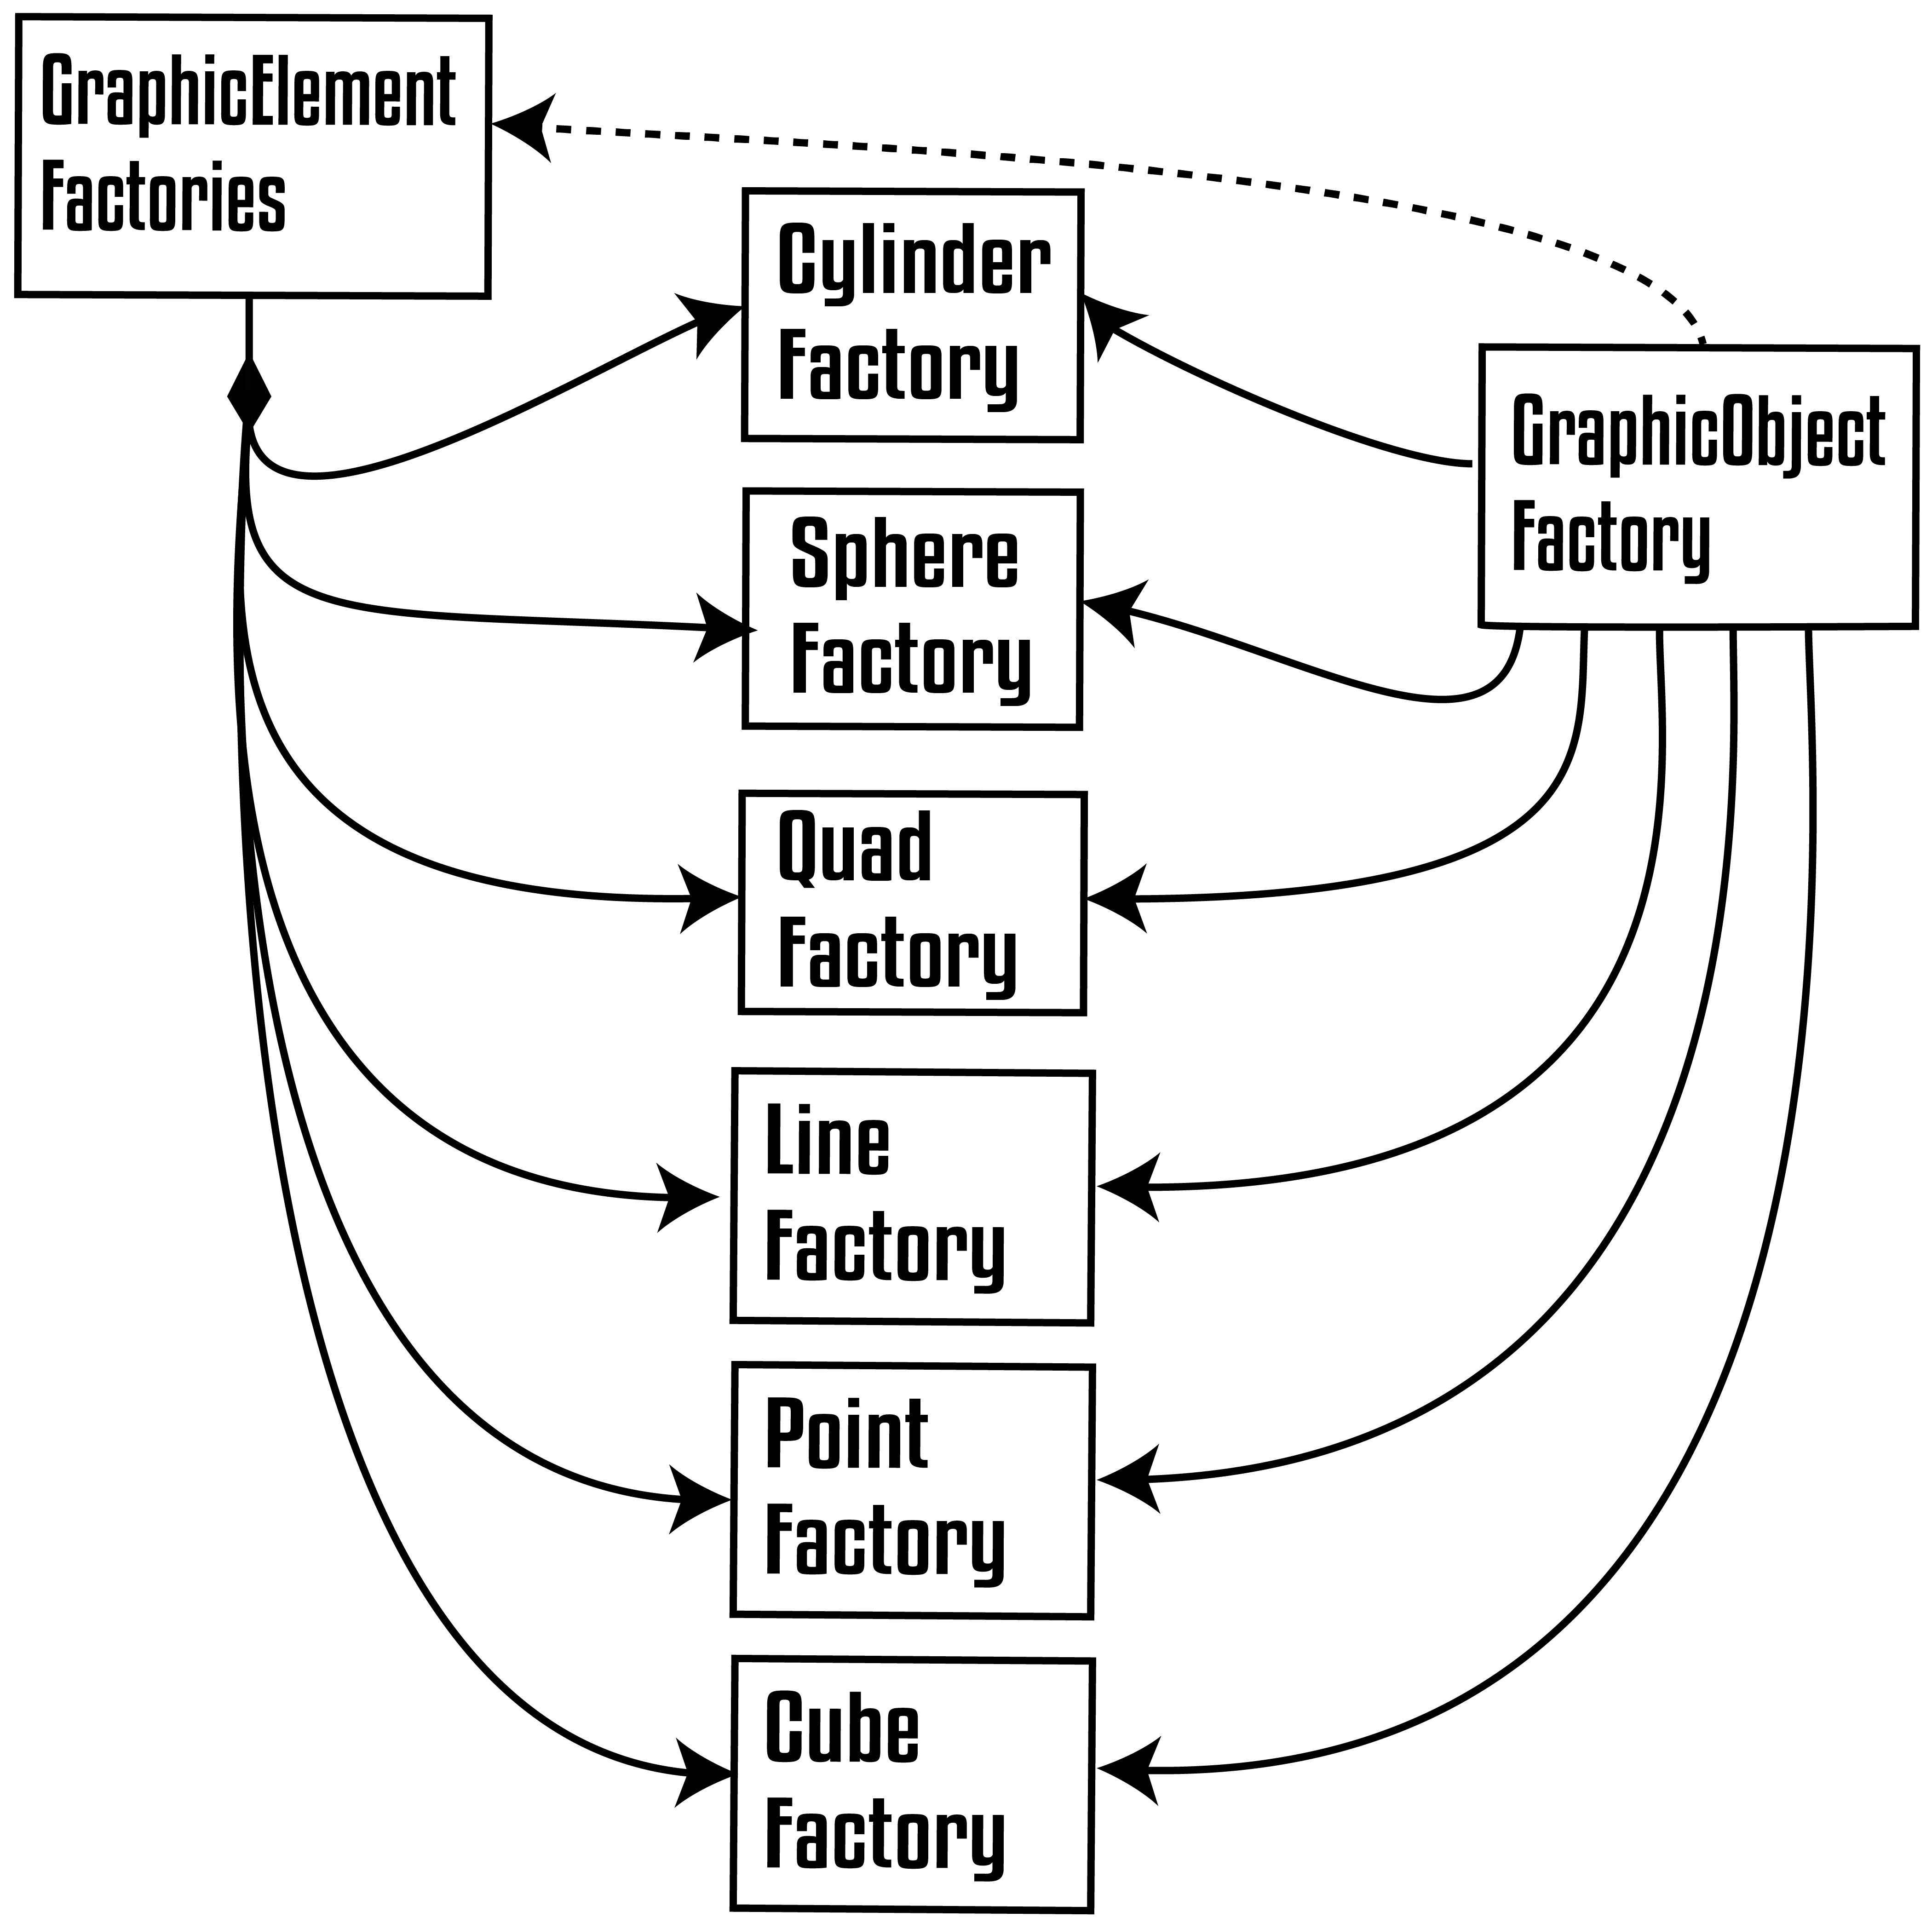
\includegraphics[width=0.5\linewidth]{Figures/GraphicElementFactories@16x.png} \\
		(c) Fábricas de objetos gráficos & (d) Fábricas de elementos gráficos \\[6pt]
		\multicolumn{2}{c}{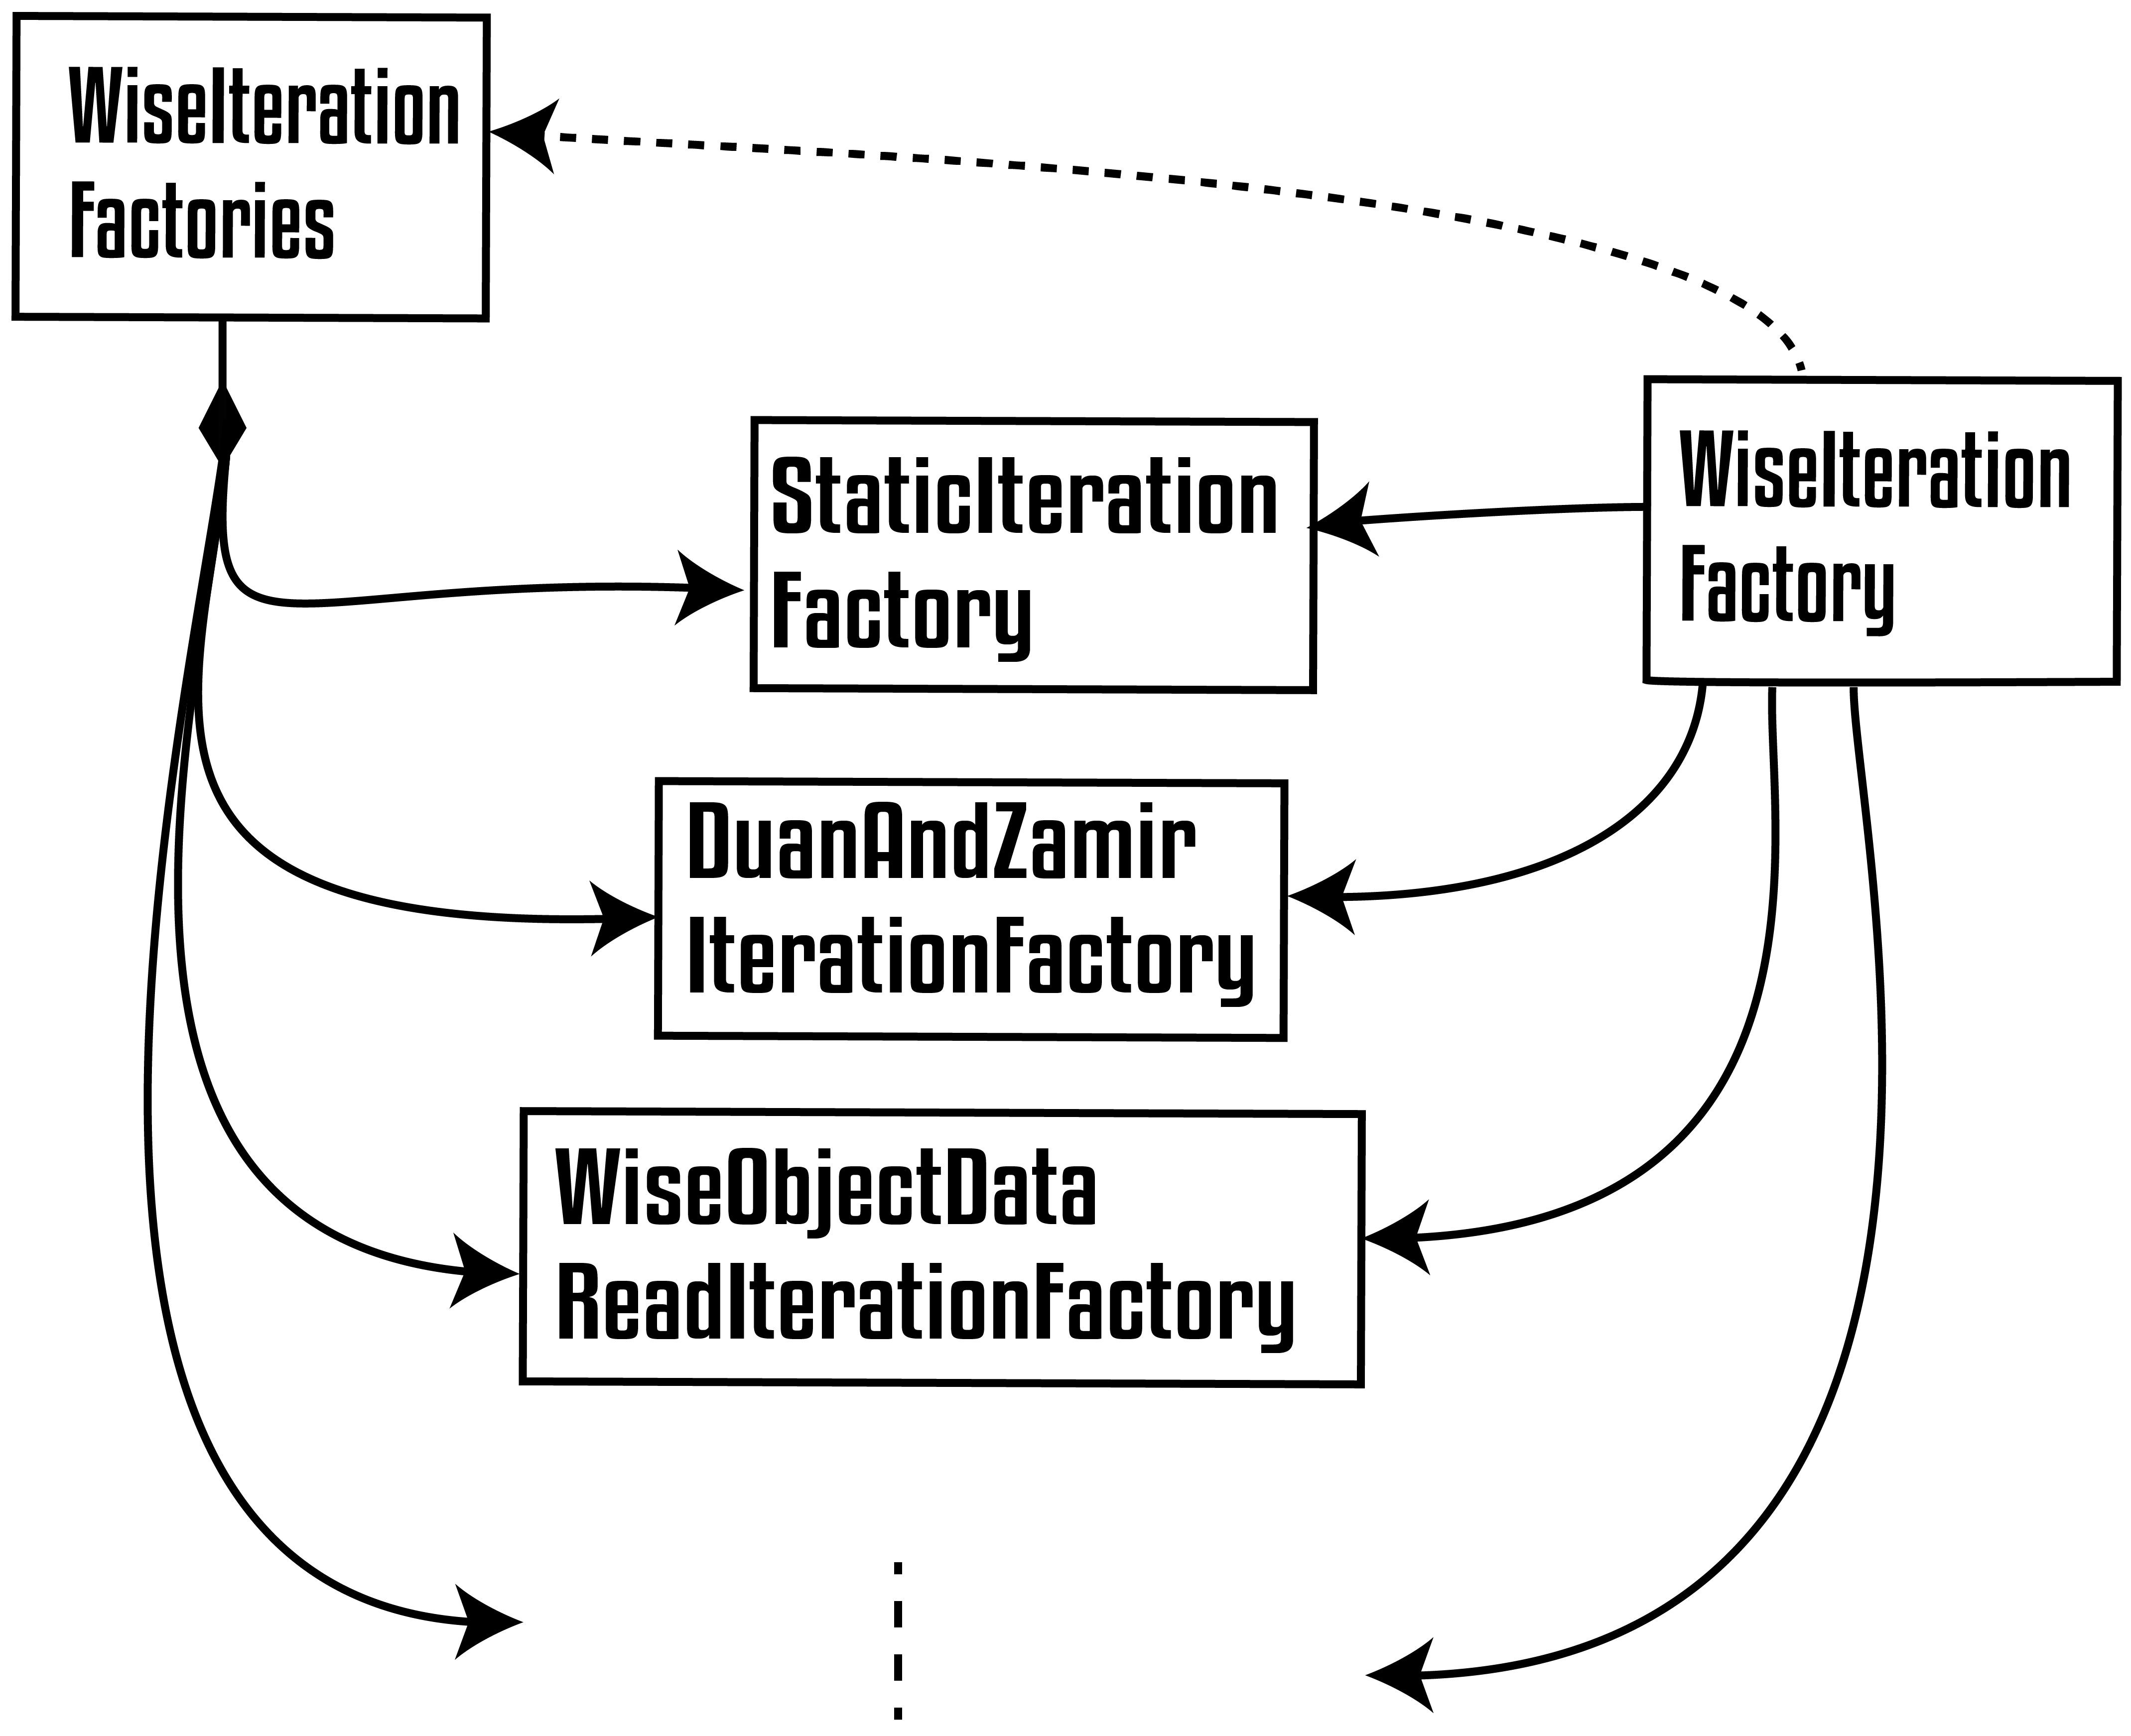
\includegraphics[width=0.5\linewidth]{Figures/WiseIterationFactories@16x.png} }\\
		\multicolumn{2}{c}{(e) Fábricas de iteração}
	\end{tabular}
	\caption{Todas as fábricas que compõem uma fábrica de projeto.}
	\label{tab:factories} 
\end{figure}

As fábricas de iteração descritas na Figura~\ref{tab:factories} foram criadas para resolver o modelo matemático descrito na Seção~\ref{sec:modelo_matematico} e extrair o seu resultado. A fábrica de iteração estática \textit{StaticIterationFactory} é uma fábrica que não altera o objeto inteligente no processo de iteração, esta é a única classe de iteração que pode ser utilizada em mais de um tipo de objeto, podendo ser executada em qualquer tipo de objeto inteligente.

O modelo do escoamento pulsátil proposto está presenta na fábrica de iteração \textit{DuanAndZamirIterationFactory}, esta fábrica é responsável por utilizar a estrutura de uma árvore arterial \textit{WiseArteryTree} e aplicar o modelo matemático. Finalmente, a fábrica de iteração \textit{WiseObjectDataReadIterationFactory} é uma fábrica responsável por armazenar os resultados obtidos a cada iteração e armazenar em uma estrutura do tipo \textit{WiseMesh}.

%--------------------------------------------------------------------------------%
\subsection{THREADS INTELIGENTES}\label{sec:threads}

Até o momento as estruturas foram construídas utilizando conceitos padrões da linguagem C++, herança de propriedades através do polimorfismo, ponteiros, classes virtuais e fábricas dinâmicas. Nesta seção o conceito de programação paralela e divisão de tarefas entre threads acoplado à ferramenta computacional é proposto. Observou-se que as estruturas possuem comportamentos padronizados e que um objeto inteligente é autônomo, ele sozinho é capaz de se armazenar, reconstruir, iterar e ocasionalmente se desenhar. Imaginando um cenário em que diversos objetos inteligente estão iterando, as tarefas foram dividas em três tipos de \textit{Threads}, primeiramente trabalhos de leitura e escrita, em seguida a iteração dos objetos. Desta forma computadores \textit{multi-thread} podem fazer uso de suas threads e permitir que mais de um objeto realize suas tarefas por vez.

Ao longo da pesquisa esta estrutura foi agregada as bibliotecas comuns do Qt 5.15.0 \cite{QTClasses}, em um primeiro momento para facilitar a visualização dos resultados através dos elementos gráficos de interface de usuários disponibilizados. Em seguida, permitiu o processamento de elementos de forma paralela. Com isso um modelo que suportasse o processamento distribuído utilizando classes \textit{QThreads} que possuem tarefas concorrentes foi construído.


\begin{figure}[!htbp]
	\centering
	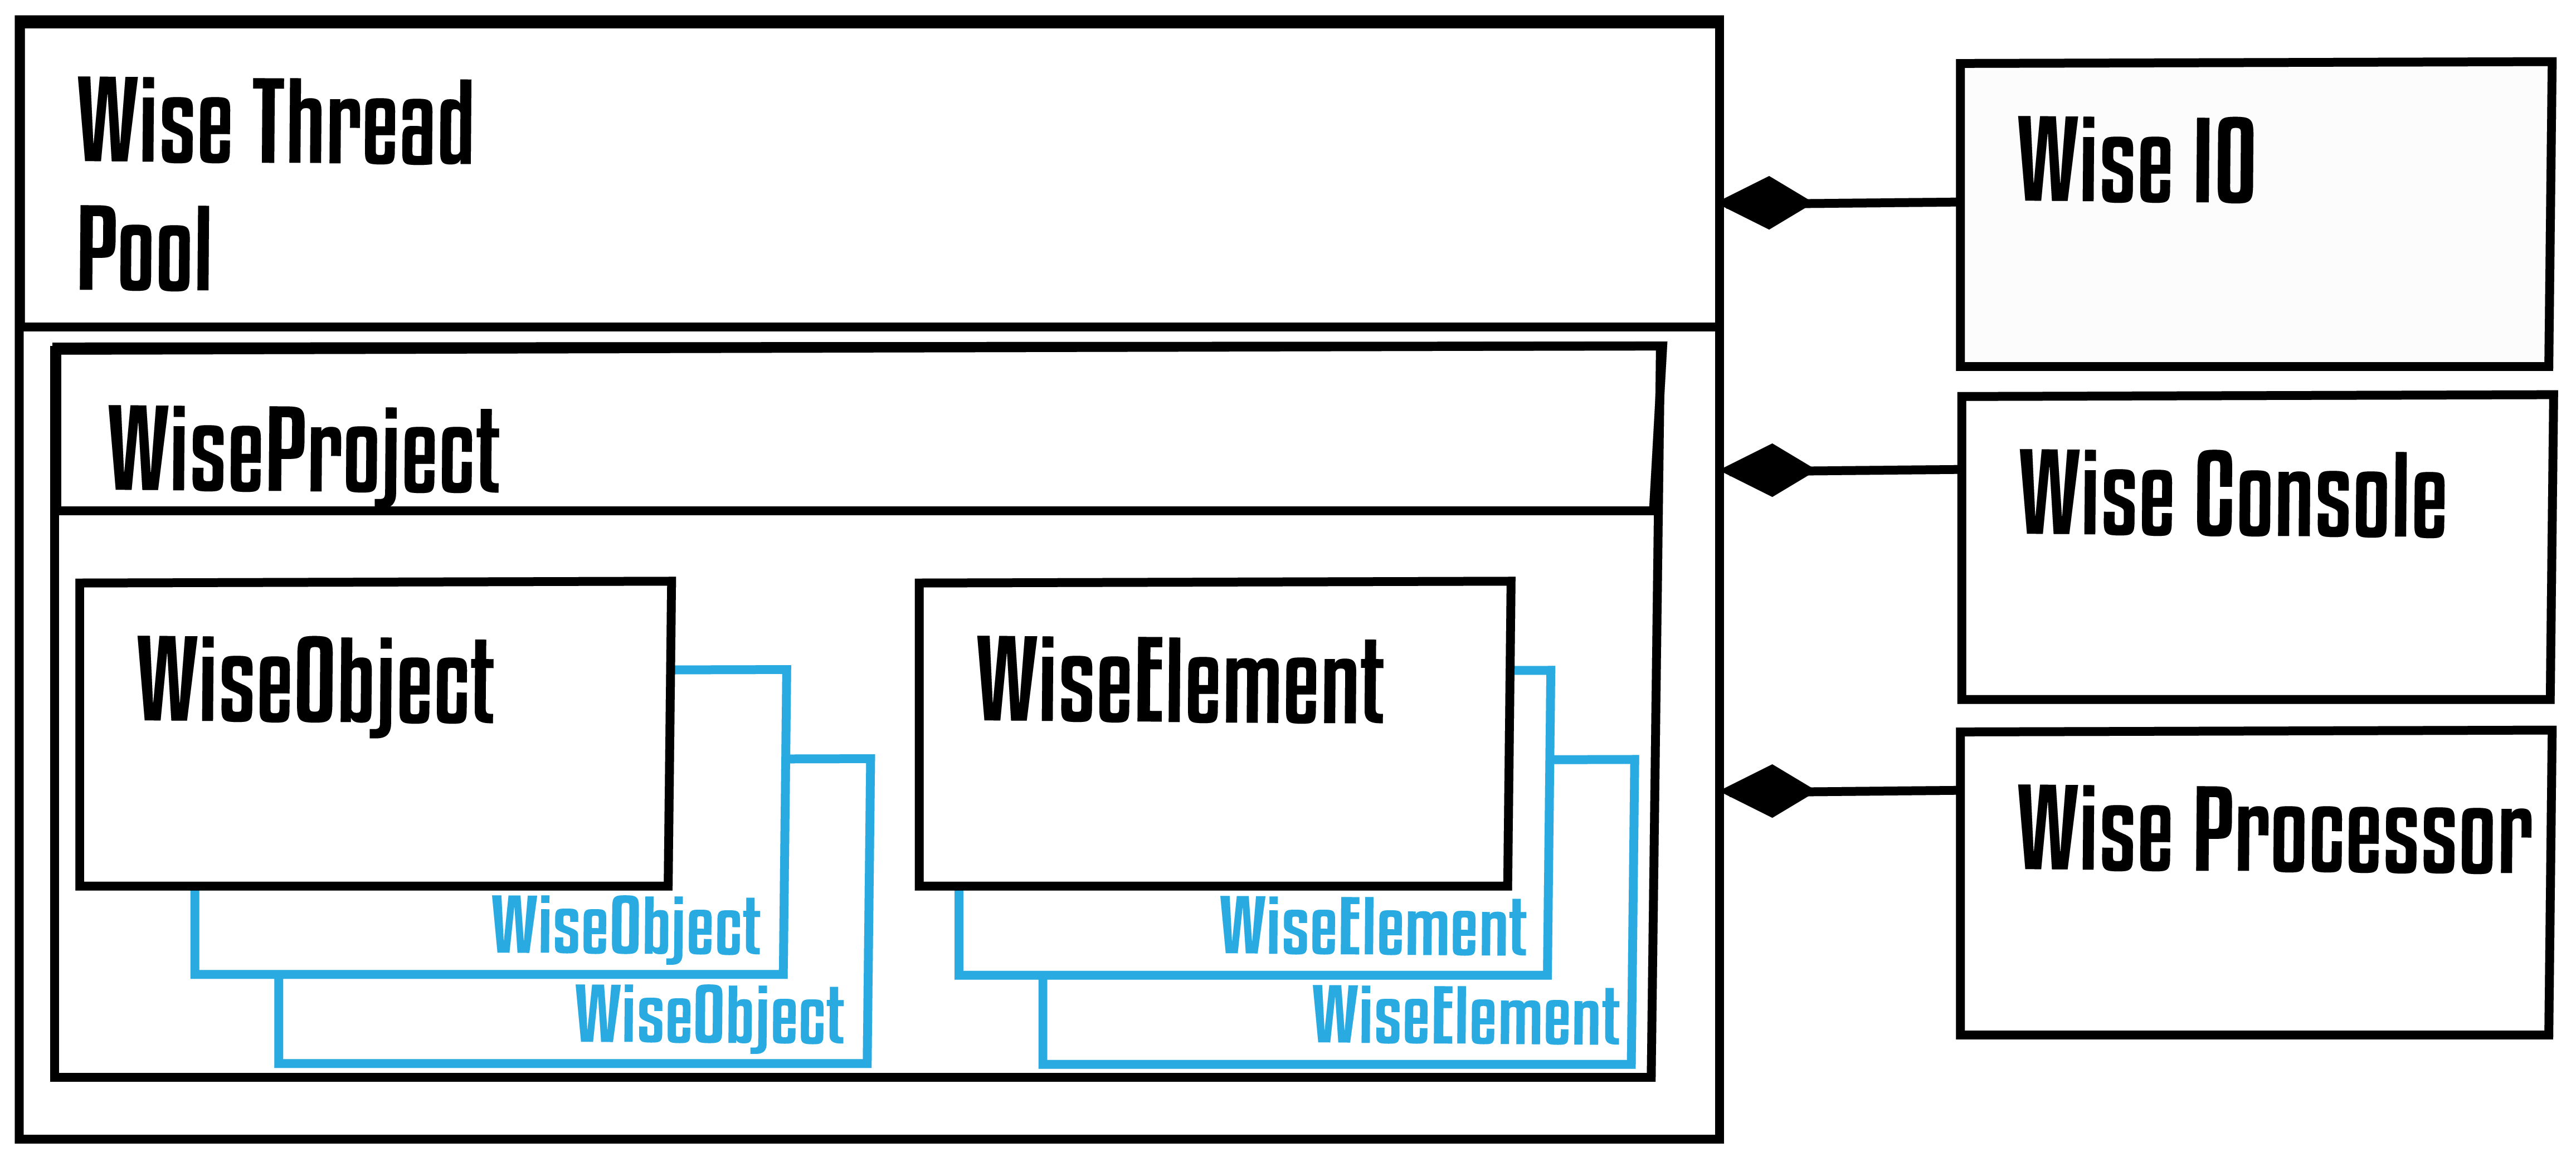
\includegraphics[width=\linewidth]{Figures/WiseThreadPool@16x.png}
	\caption{Modelo de Threads. \textit{WiseThreadPool}, responsável por orquestrar o funcionamento das demais threads, bem como os objetos contidos em um projeto \textit{WiseProject}. \textit{WiseIO}, thread responsável por processos de leitura e escrita. \textit{WiseConsole}, thread responsável por interpretar os comandos de texto e os traduzir-los na chamada de métodos. \textit{WiseProcessor}, thread responsável por realizar o método iterativo de um objeto inteligente \textit{WiseObject}}
	\label{fig7:threads}
\end{figure}

As tarefas se dividem em três principais grupos: tarefas auxiliares, tarefas de leitura/escrita e trabalhos de iteração. O principal trabalho auxiliar é interpretar os comandos recebidos pelo programa e então criar a instância de trabalho inteligente \textit{WiseJob}. Sendo os grupos de tarefas mais custosos os de tarefas de escrita/leitura e iteração, se dividiram em threads específicas, \textit{WiseIO} e \textit{WiseProcessor} respectivamente.

Os objetos distribuídos \textit{threads} contidos na Figura~\ref{fig7:threads} possuem um ciclo próprio, portanto executam tarefas assíncronas e precisam de tratamento adequado. O sistema de sinais e fendas disponibilizado pelas bibliotecas comuns do Qt permitem que as \textit{threads} se comuniquem assincronamente através do envio de mensagens. Estas mensagens são chamadas de trabalhos inteligentes \textit{WiseJobs}, cada uma possuindo sua atividade relacionada e objeto relacionado. Uma vez criados, os trabalhos inteligentes são alocados à sua respectiva categoria de \textit{thread} passando por um balanceamento executado pelo gerenciador de threads \textit{WiseThreadPool}. Enquanto o processamento é feito, todos os dados relativos ao processamento são bloqueados, isso previne a sobrescrita de dados quando há mais de uma thread trabalhando.

O gerenciador de threads \textit{WiseThreadPool} é composto por \textit{threads} que executam os trabalhos e por projetos inteligentes \textit{WiseProject} que criam trabalhos \textit{WiseJobs}. Ao executar um comando de texto, a linha de entrada será recebida pelo gerenciador e o primeiro trabalho inteligente \textit{WiseJob} será criado. Em seguida será interpretado por \textit{threads} do grupo de tarefas auxiliares \textit{WiseConsole}, caso seja um trabalho de leitura, escrita ou iteração um trabalho inteligente associado será criado e enviado ao gerenciador de \textit{threads}. Caso não seja um trabalho desses tipos ele será executado na thread atual e o trabalho inteligente finalizado. O console inteligente \textit{WiseConsole} funciona como interpretador principal dos comando e das mensagens, ao receber uma linha de texto este objeto irá analisar seu conteúdo e executar a ação correspondente.

\begin{figure}[!htbp]
	\centering
	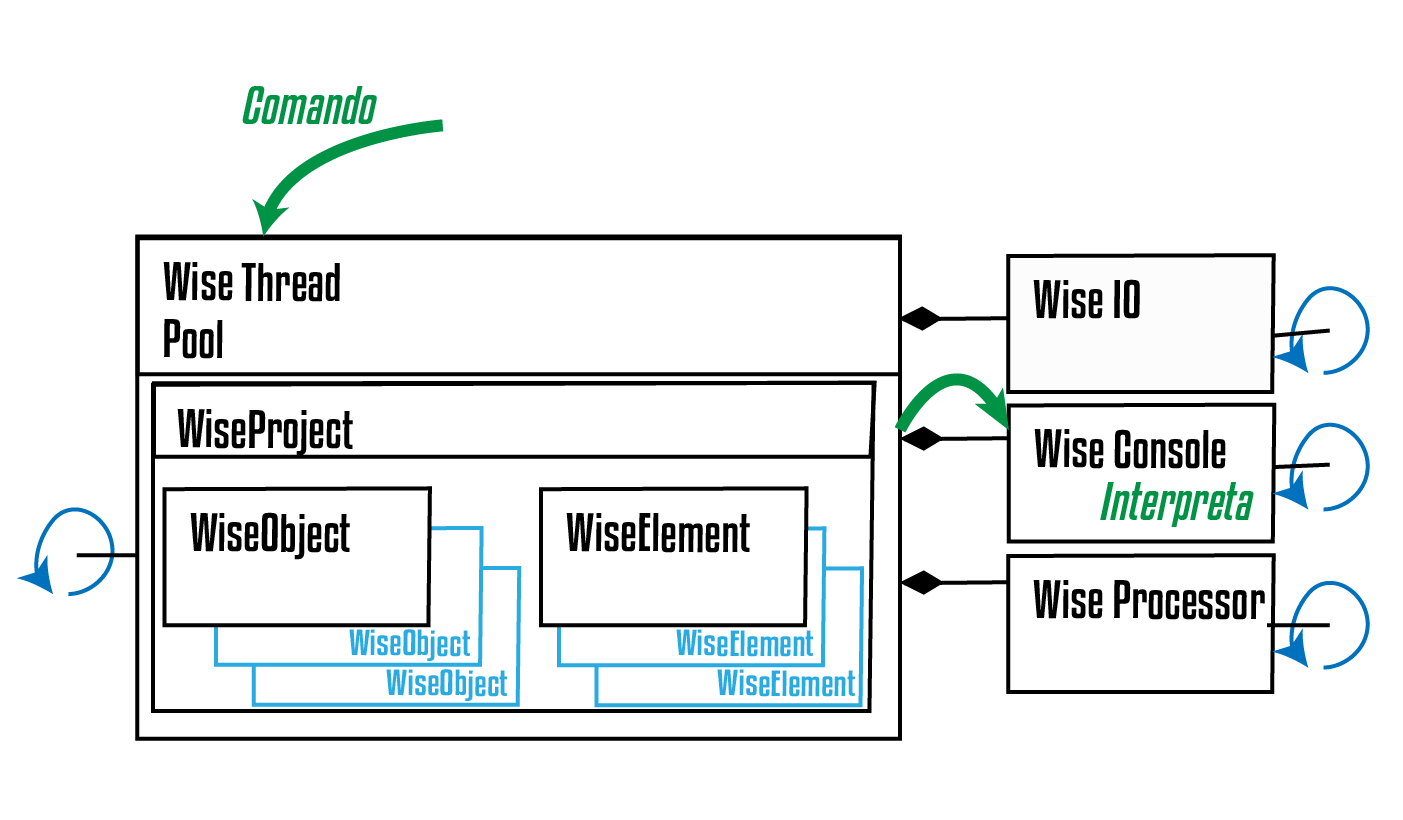
\includegraphics[width=\linewidth]{Figures/WiseThreaPoolCMD.png}
	\caption{Modelo de Threads ao receber uma linha de comando da interface de usuário.}
	\label{fig8:threads}
\end{figure}

Quando se trata de um comando de escrita ou leitura, a thread \textit{WiseIO} é utilizada, ao receber esse tipo de comando o console inteligente irá listar o trabalho no gerenciador de threads \textit{WiseThreadPool}. O gerenciador irá balancear as requisições entre as threads e em seguida o gerenciador de threads irá aguardar uma mensagem, indicando o final da execução do trabalho. Quando um objeto inteligente \textit{WiseObject} é iterado um elemento inteligente é criado na estrutura \textit{Freezer}, gerando uma requisição através de um trabalho inteligente. Portanto a thread \textit{WiseIO} é muito utilizada no ciclo de vida de um elemento inteligente, gerenciando o processo de armazenamento e reconstrução do elemento. É esta estrutura que efetivamente aquece e resfria elementos inteligentes.

\begin{figure}[!htbp]
	\centering
	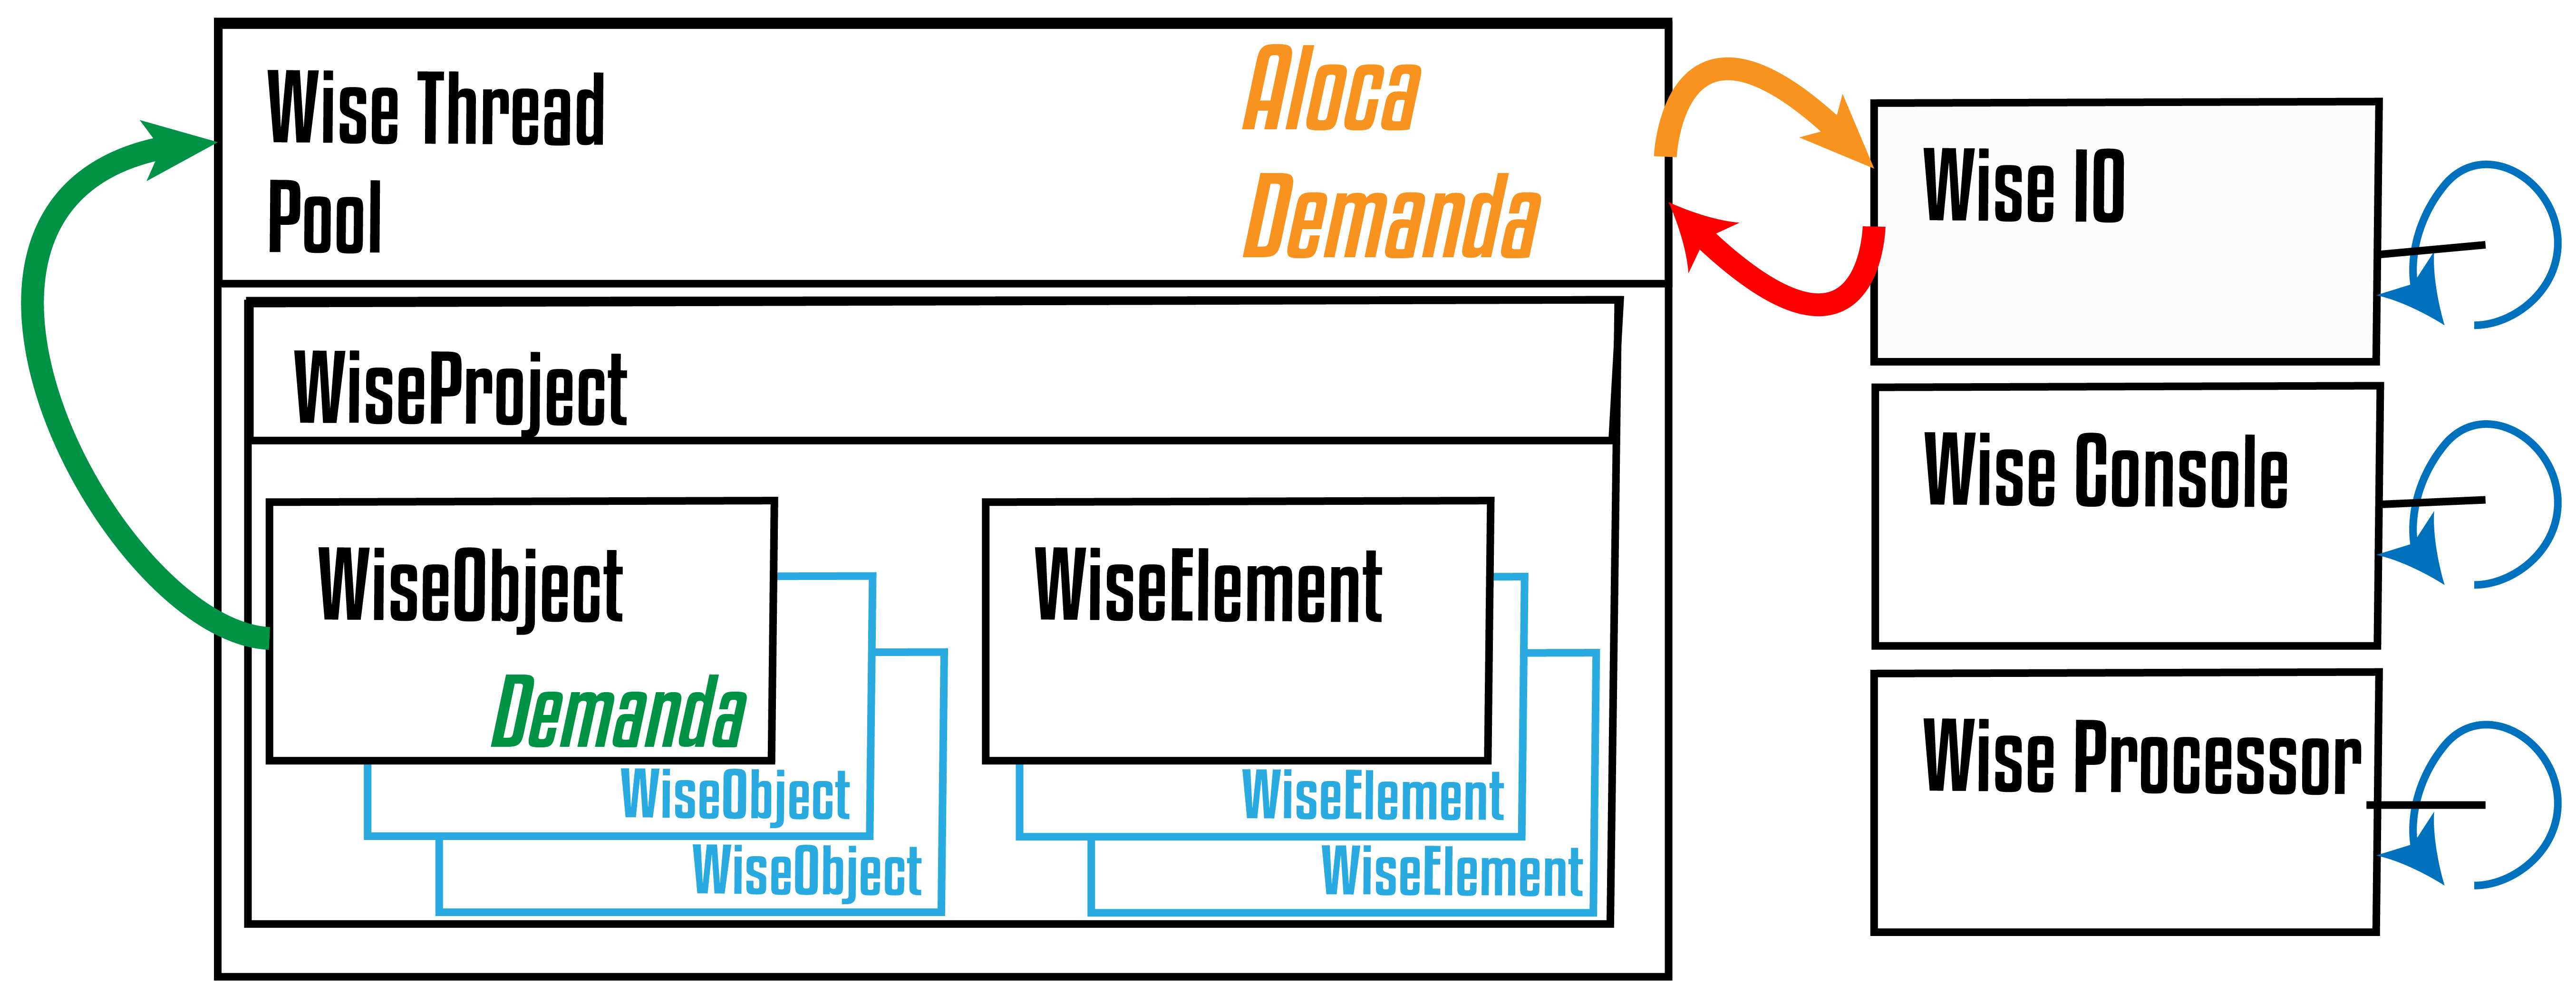
\includegraphics[width=\linewidth]{Figures/WiseThreadPoolHeating@16x.png}
	\caption{Modelo de Threads ao receber um comando de escrita/leitura.}
	\label{fig9:threads}
\end{figure}

Os trabalhos de iteração funcionam da mesma forma que as de leitura ou escrita, entretanto são enviadas a threads \textit{WiseProcessor}. Estas \textit{threads} não possuem lógicas muito complexas, elas são responsáveis apenas por gerenciar os objetos e executar os métodos requisitados, por este motivo os objetos inteligentes e elementos inteligentes possuem métodos abstratos e seguem esses conjuntos de regras, para que uma estrutura que desconheça o seu funcionamento ou suas estruturas internas sejam capazes de executar métodos padrões. 

Mesmo com a arquitetura de threads inclusa na ferramenta computacional ainda é possível que ela seja executada em plataformas de thread única, neste caso mais threads inteligentes não farão diferença, pois apesar dos trabalhos ainda serem dividos em threads diferentes, elas serão executadas no mesmo núcleo de processamento. As threads inteligentes têm um impacto maior nas atividades de escrita e leitura, isto porque o objeto inteligente está divido em várias estruturas menores que são armazenadas e acessadas constantemente, principalmente no caso de uma animação gráfica.

Ainda dentro do gerenciador de threads inteligentes existem quatro listas de espera:

\begin{itemize}
	\item \textbf{Pre-Queue (Pre-Q)}: Lista de pré-seleção. Nesta estrutura os trabalhos são agrupados por grupo de trabalho e ordenadas por data de criação.
	\item \textbf{Queue (Q)}: Lista de espera, para trabalhos que aguardam sua alocação em threads adequadas.
	\item \textbf{Running}: Lista de trabalhos que já foram enviados às suas respectivas threads e aguardam resposta.
	\item \textbf{Finished}: Lista de trabalhos que já terminaram o seu ciclo de execução.
\end{itemize}

No momento de criação os objetos são adicionados à lista \textit{Pre-Q}. A cada ciclo da thread \textit{WiseThreadPool} trabalhos da lista \textit{Pre-Queue} são enviados a lista de espera \textit{Queue}, os trabalhos de cada carga de trabalho são selecionados e enviados caso não haja pré-requisitos. Como exceção está a carga de trabalho utilizada pela ferramenta para armazenar e recuperar objetos rapidamente, para isto foi reservada a carga de trabalho $w = 6$.

Os trabalhos na lista de espera \textit{Queue} são balanceados entre as threads disponíveis utilizando uma distribuição uniforme. Uma vez alocados, os trabalhos passam para a lista de trabalhos \textit{Running}, que contém os trabalhos em execução.

Finalmente, ao final da execução em uma thread separada, a estrutura armazena os trabalhos finalizados em uma lista \textit{Finished}, estes finalizaram seu processamento em uma thread concorrente e uma resposta foi recebida pelo gerenciador de threads.

%--------------------------------------------------------------------------------%
\subsection{TRABALHOS INTELIGENTES}\label{sec:trabalhos}

Para que a comunicação entre as threads inteligentes \textit{WiseThreads} seja feita de forma padronizada e possa ser estendida futuramente. Ao receber alguma demanda, o gerenciador de thread inteligentes \textit{WiseThreadPool} irá criar um objeto do tipo \textit{WiseJob}, este objeto contém os seguinte parâmetros:

\begin{itemize}
	\item \textbf{ID}: Número de identificação único.
	\item \textbf{Workload}: Núemero de carga de trabalho.
	\item \textbf{Arg}: Cadeia de caracteres opcional, pode conter parâmetros para a execução do trabalho.
	\item \textbf{Type}: Tipo de trabalho.
	\item \textbf{Status}: Estado do trabalho.
	\item \textbf{Antecessors}: Lista de trabalhos que antecedem este na ordem de chamada.
	\item \textbf{Pre-requisites}: Lista de trabalhos que antecedem este na ordem de execução, ou seja, precisam ser finalizados antes.
	\item \textbf{Ponteiros}: O trabalho do tipo \textit{WiseJob} pode ter um ponteiro para estruturas da ferramenta computacional.
\end{itemize}

O número de identificação do trabalho é único e incremental, a carga de trabalho representa o grupo em que o trabalho irá executar. Ao executar a leitura de um arquivo de entrada, cada linha do arquivo irá ser interpretada como um comando e adicionada ao mesmo grupo de trabalho e vinculada ao último comando pela lista de antecessores \textit{Antecessors}, desta forma é garantido que eles serão executados em ordem.

O tipo \textit{Type} do trabalho inteligente é um identificador dado ao trabalho após sua interpretação inicial. Este identificador permite às threads determinar qual a composição do objeto e quais parâmetros para execução foram preenchidos, como ponteiros e linhas de entrada. 

\begin{figure}[!htbp]
	\centering
	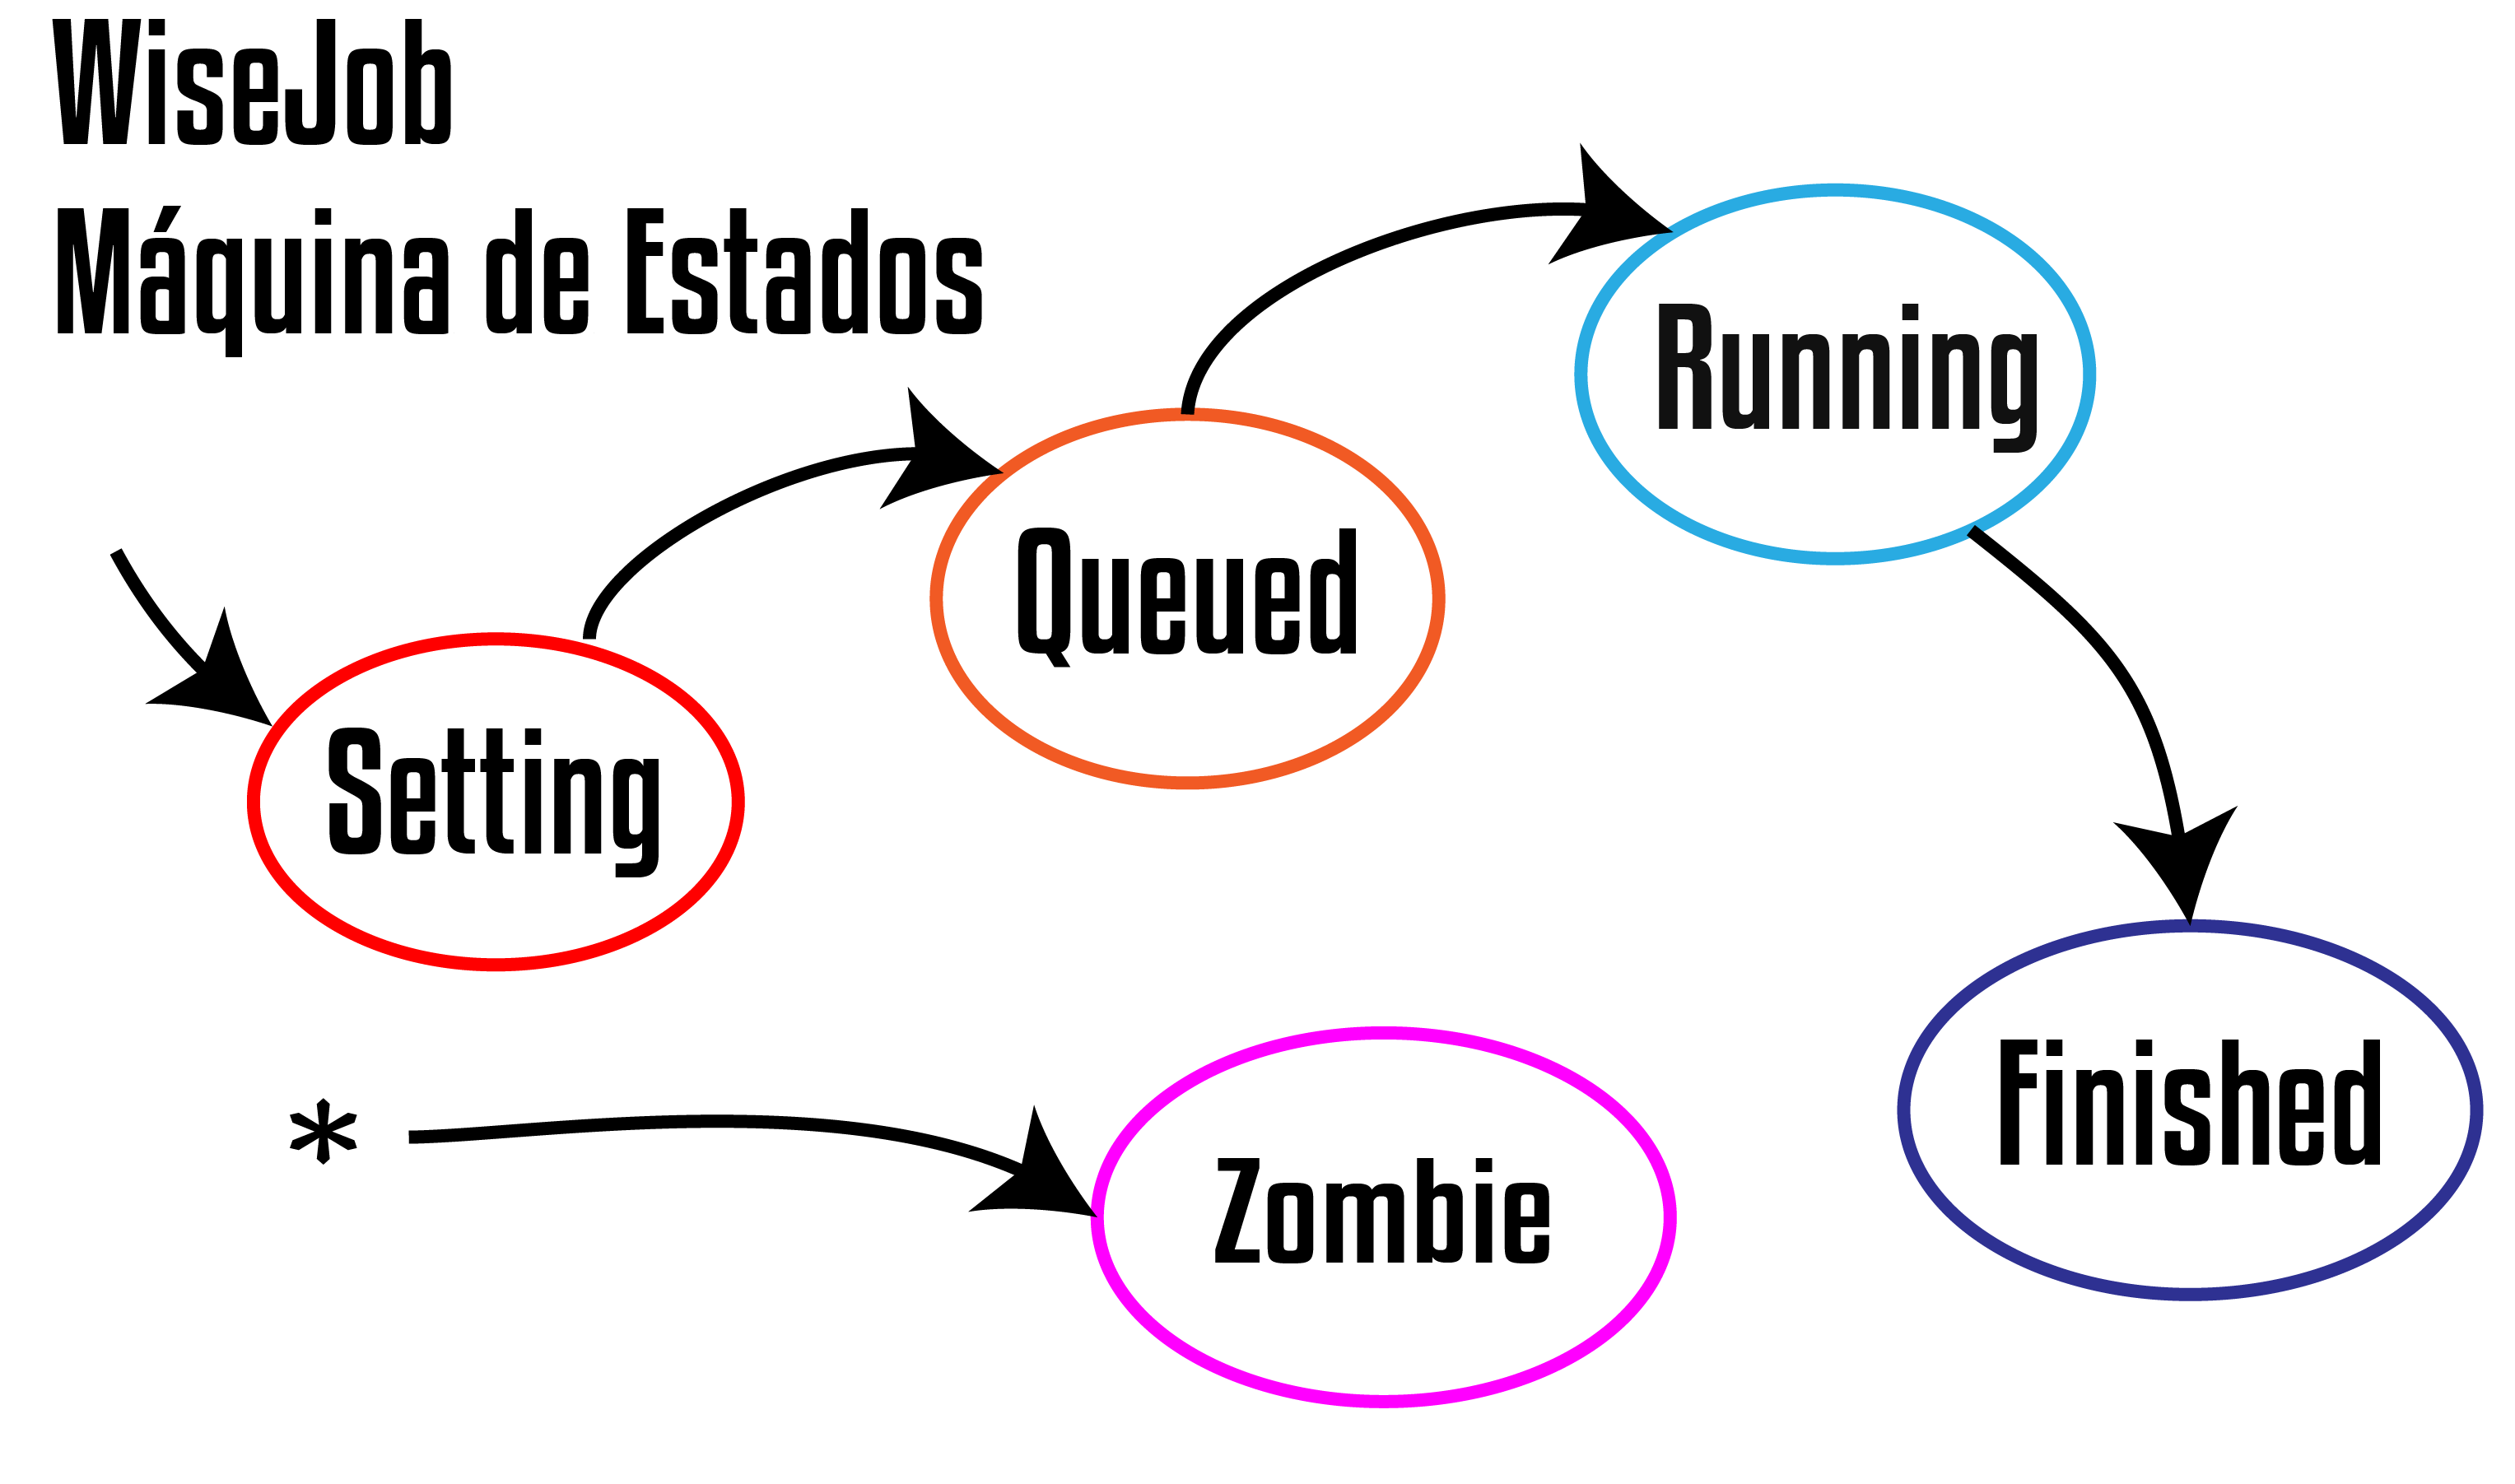
\includegraphics[width=\linewidth]{Figures/WiseJobStatus@16x.png}
	\caption{Máquina de estados utilizadas por trabalhos inteligentes \textit{WiseJobs}.}
	\label{fig9:wise_jobs}
\end{figure}

Os estados de um trabalho inteligente são ditados pela sua máquina de estados representada na Figura~\ref{fig9:wise_jobs}. Os estados desta máquina indicam em qual estrutura da \textit{WiseThreadPool} o trabalho está e se seu funcionamento é adequado. O estado \textit{Setting} indica que o trabalho foi criado e está na lista de seleção \textit{Pre-Q}; O estado \textit{Queued} significa que o trabalho foi adicionado à fila de espera e aguarda execução; O estado \textit{Running} indica que o trablho está sendo executado; O estado \textit{Finished} indica que o trabalho foi finalizado corretamente; E, o estado \textit{Zombie} indica que o trabalho não foi finalizado corretamente. 

Os objetos de trabalho inteligente servem como mensagens de comunicação entre as threads. Através desta estrutura objetos do tipo \textit{QObject} podem se comunicar e executar a requisição de trabalhos complexo. Isto foi feito para permitir que estruturas \textit{QWidget}, que são elementos gráficos da interface de usuário e herdam da classe \textit{QObject}, pudessem enviar mensagens diretamente ao gerenciador de threads.

%-------------------------------------------------------------------------------------------%
\section{INTERFACE DE USUÁRIO}\label{sec:userinterface}

Nesta seção apresentam-se detalhes da interface escolhida para facilitar o uso da ferramenta computacional. A interface de usuário foi concebida para permitir o controle de todas as estruturas descritas na Seção~\ref{sec:estrutura} com todos os seus recursos gráficos extraídos. A interface se divide em dois ambientes: Um console, que permite uma interação textual e acesso as mesmas funcionalidades de iteração; E uma janela com elementos gráficos capazes de exibir os resultados gráficos obtidos. 

\begin{figure}[!htbp]
	\centering
	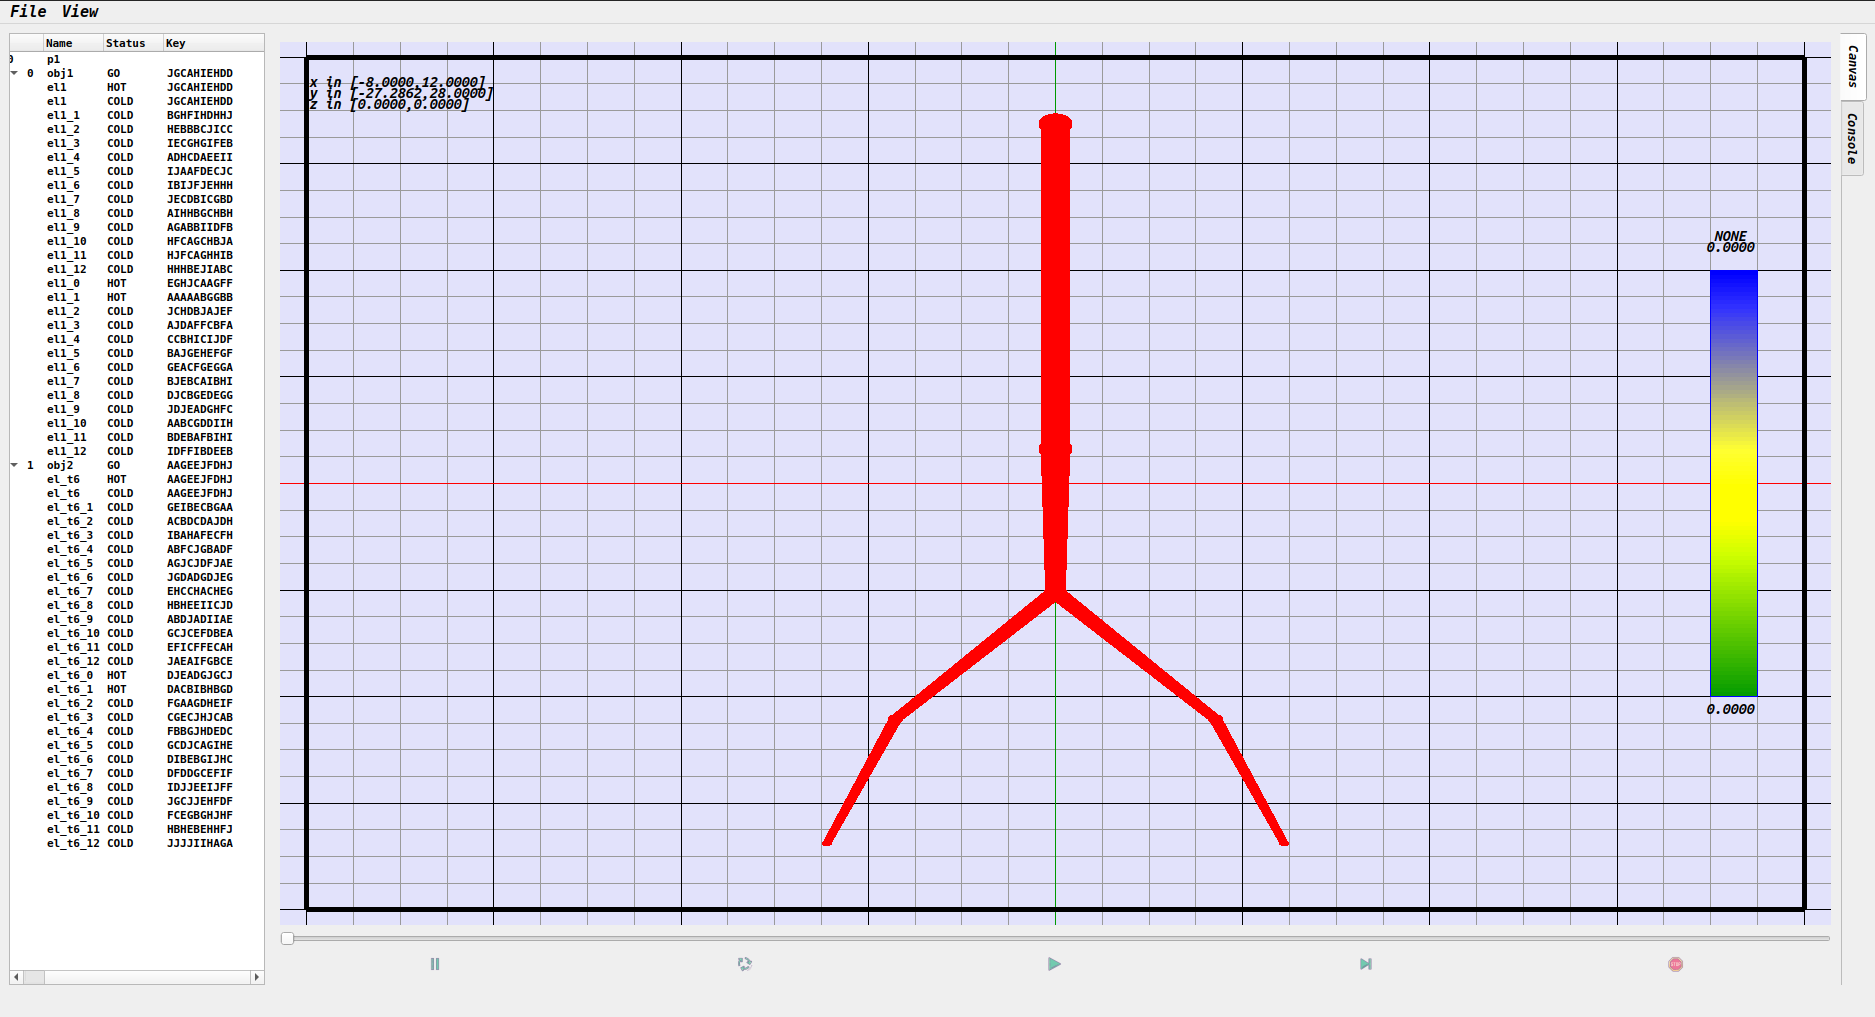
\includegraphics[width=\linewidth]{Figures/IGU_002.png}
	\caption{Interface de usuário gráfica.}
	\label{fig10:UI}
\end{figure}

Ambas as interfaces foram construídas para manipular objetos inteligentes e suas estruturas, por isto ambas possuem instâncias do gerenciador de threads inteligentes descritos na Seção~\ref{sec:estrutura}. O console se trata de um envio direto de mensagens para a thread \textit{WiseConsole}, que é efetivamente o console. Nas próximas seções os diferentes ambientes da ferramenta computacional serão descritos. Cada ambiente representa um projeto \textit{Qt}/\textit{C++} distinto, entretanto dividem as mesmas classes.

%-------------------------------------------------------------------------------------------%
\section{CONSOLE}\label{sec:console}

O ambiente de console da ferramenta computacional consiste em um projeto \textit{Qt}/\textit{C++} sem interface gráfica. O projeto foi intitulado \textit{InGU} ou \textbf{I}terador \textbf{n}ão-\textbf{G}ráfico \textbf{U}niversal, porque o ambiente apesar de não conter os elementos para a visualização dos elementos gráficos, é capaz de criar as estruturas gráficas para visualização futura.  No console as bibliotecas gráficas do OpenGL não foram incluídas no processo de compilação, portanto ambientes sem recursos gráficos são capazes de compilar e executar a ferramenta computacional através deste ambiente.

\begin{figure}[!htbp]
	\centering
	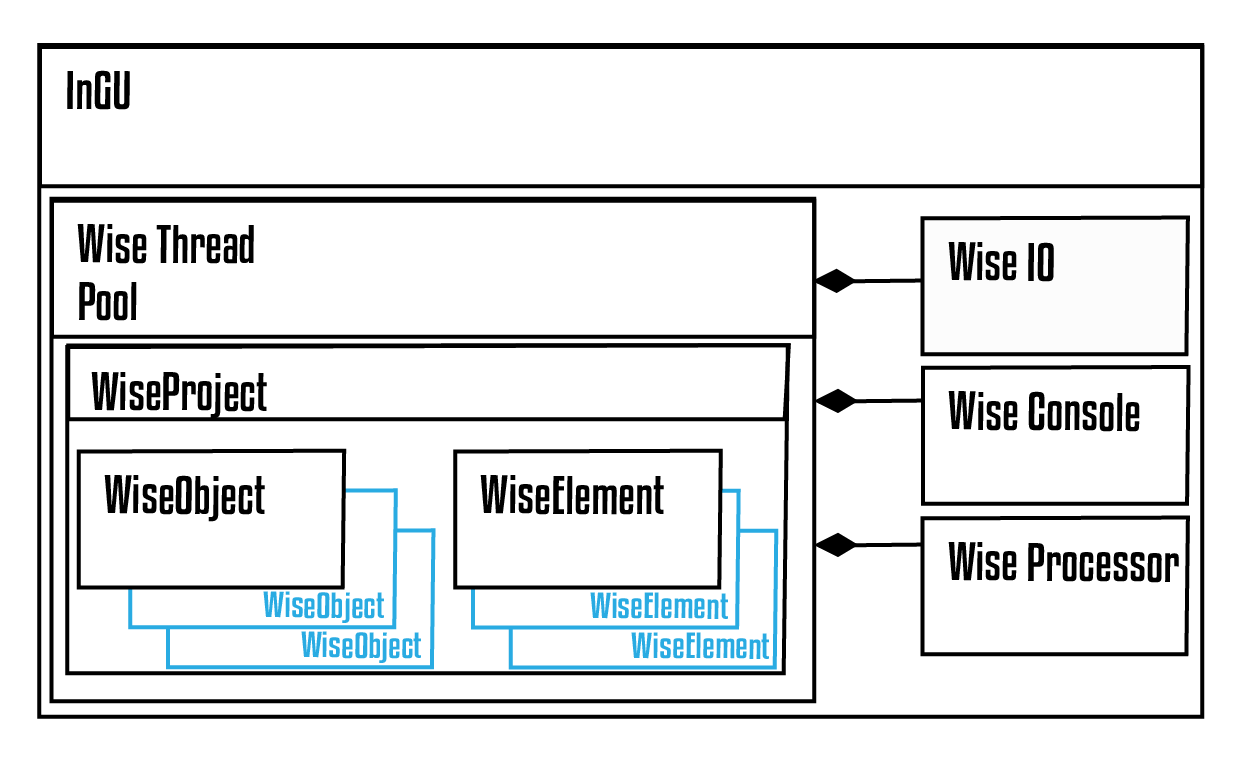
\includegraphics[width=\linewidth]{Figures/InGU.png}
	\caption{Estrutura do projeto que compõe o ambiente computacional InGU.}
	\label{fig10:console}
\end{figure}

No anexo estão as sequências de instruções necessárias para compilar todos os projetos da ferramenta computacional. Ao ser compilado, um executável InGU contendo o projeto console é gerado. Ao ser executado, o console corresponde do sistema operacional irá ser aberto com o cabeçalho da ferramenta e aguardará entrada de texto.

\begin{figure}[!htbp]
	\centering
	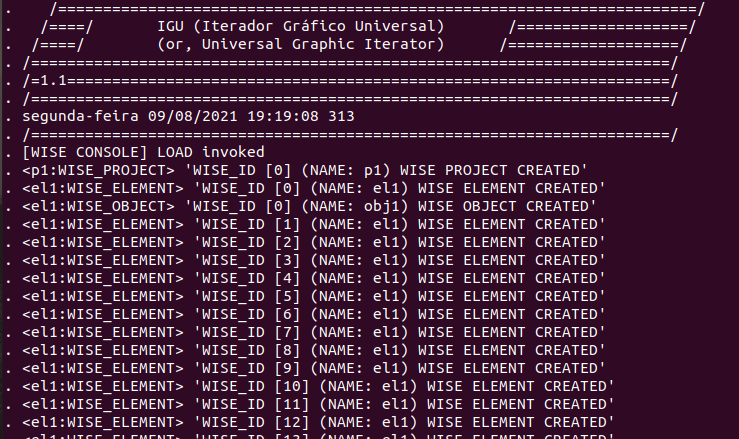
\includegraphics[scale=0.45]{Figures/InGU_console.png}
	\caption{Captura de tela com a execução do ambiente computacional InGU em um console.}
	\label{fig11:ajuda}
\end{figure}

Para executar um comando, basta inserir uma linha de texto e apertar a tecla \textit{Enter}.  Ao capturar a linha de texto, o programa de console irá na verdade redirecionar o comando para a estrutura \textit{WiseThreadPool}, que por sua vez irá alocar uma thread do tipo \textit{WiseConsole} para interpretar a mensagem. Este comportamento é o mesmo apresentado na Seção~\ref{sec:threads}. Uma lista de comandos foi disponibilizada e está acessível através do comando \textit{help}. Ao enviar este comando para o console uma lista com todos as possíveis entradas será exibida. Nas próximas seções estes comandos, suas entradas, seu escopo e thread responsável serão descritos, esta thread irá executar a tarefa. 

%--------------------------------------------------------------------------------%
\subsection{AJUDA}\label{sec:help}

O comando de ajuda é o primeiro comando da interface e foi feito para listar todas as entradas possíveis do programa. Ao receber este comando a thread \textit{WiseConsole} envia o texto pré-definido com todos os comandos.

\begin{center}
	\begin{table}[!htbp]
		\begin{tabular}{|c|m{0.6\textwidth}|}
			\hline
			\textbf{Linha de Comando} & \multicolumn{1}{c|}{help} \\
			\hline
			\textbf{Escopo} & \multicolumn{1}{c|}{nenhum} \\
			\hline
			\textbf{Thread Responsável} & \multicolumn{1}{c|}{WiseConsole} \\
			\hline
			\textbf{Entrada} & Nenhuma \\
			\hline
		\end{tabular}
		\caption{Descrição do comando ajuda.}
		\label{tab:help}
	\end{table}
\end{center}

Ao executar o comando, o usuário receberá uma lista de comandos divididos em escopos específicos. Os escopos foram criados para agrupar comandos por área de atuação, comandos auxiliares, como o comando de ajuda, são os comandos que não alteram as estruturas e exibem informações auxiliares ao usuário.


\begin{figure}[!htbp]
	\centering
	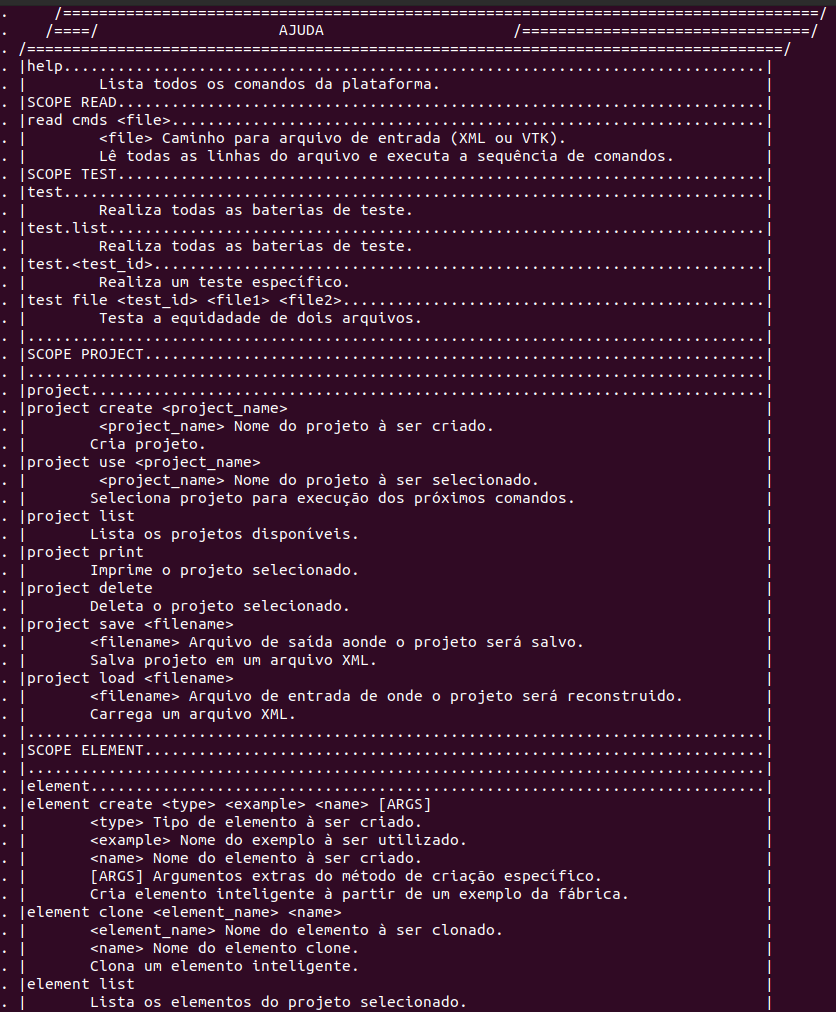
\includegraphics[scale=0.45]{Figures/InGU_help.png}
	\caption{Captura de tela com a execução do ambiente computacional InGU em um console.}
	\label{fig10:ajuda}
\end{figure}


%--------------------------------------------------------------------------------%
\subsection{LER ARQUIVO DE ENTRADA}\label{sec:read_cmds}


O comando ler arquivo de comandos irá receber o endereço de um arquivo local, este arquivo deve conter um comando por linha, um exemplo pode ser encontrado no Anexo~\ref{annex2}. Para este tipo de comando um \textit{WiseJob} contendo a linha de comando e qual a sequência de trabalhos que deve ser executada. Por se tratar de uma leitura de arquivo de comando, a thread \textit{WiseIO} será responsável por ler o arquivo e criar os trabalhos com os comandos subsequentes. Estes novos comandos irão passar novamente pela interpretação de uma thread do tipo \textit{WiseConsole} e em seguida executados.

\begin{center}
	\begin{table}[!htbp]
		\begin{tabular}{|c|c|m{0.6\textwidth}|}
			\hline
			\textbf{Linha de Comando} & \multicolumn{2}{c|}{read cmds <file>} \\
			\hline
			\textbf{Escopo} & \multicolumn{1}{c|}{READ} \\
			\hline
			\textbf{Thread Responsável} & \multicolumn{1}{c|}{WiseIO} \\
			\hline
			\textbf{Entrada} & \textbf{<file>} & Caminho para arquivo contendo sequência de comandos. \\
			\hline
		\end{tabular}
		\caption{Descrição do comando ler arquivo de comando.}
		\label{tab:read}
	\end{table}
\end{center}

%--------------------------------------------------------------------------------%
\subsection{BATERIA DE TESTES}\label{sec:test}

O ciclo principal de testes da ferramente se baseia em verificar a consistência de todas as fábricas e do fluxo principal da ferramenta computacional, exceto detalhes gráficos e do processo de iteração. Ao executar a bateria de testes todos os elementos inteligentes \textit{WiseElement} e objetos inteligentes \textit{WiseObject} disponíveis serão testados individualmente. Para isto, uma fábrica de projeto \textit{WiseProjectFactory} irá ser encarregada de criar todos os elementos e objetos inteligentes disponíveis.

Estes testes foram utilizados principalmente no momento do desenvolvimento da ferramenta e garantem que as fábricas de elementos e objetos inteligentes estão funcionando corretamente. Futuramente, caso novas estruturas sejam incluídas, estes testes garantem que todas as classes do projeto foram projetadas corretamente, com isso todas as estruturas que são carregadas pela ferramenta não perdem informação ao serem armazenadas e recuperadas, processo recorrente na ferramenta computacional. Os comandos deste tipo são de responsabilidade da thread \textit{WiseConsole}, que irá criar e executar subcomando, trabalhos \textit{WiseJob} relacionados À uma atividade superior.

\begin{center}
	\begin{table}[!htbp]
		\begin{tabular}{|c|m{0.6\textwidth}|}
			\hline
			\textbf{Linha de Comando} & \multicolumn{1}{c|}{test} \\
			\hline
			\textbf{Escopo} & \multicolumn{1}{c|}{TEST} \\
			\hline
			\textbf{Thread Responsável} & \multicolumn{1}{c|}{WiseConsole} \\
			\hline
			\textbf{Entrada} & Nenhuma \\
			\hline
		\end{tabular}
		\caption{Descrição do comando bateria de testes.}
		\label{tab:test}
	\end{table}
\end{center}

%--------------------------------------------------------------------------------%
\subsection{LISTA DE TESTES}\label{sec:test list}

O comando de listar testes irá enumerar todos os teste possíveis de serem executados pela ferramenta computacional. Assim como o comando de ajuda, este comando irá imprimir no console todas os resultados encontrados.

\begin{center}
	\begin{table}[!htbp]
		\begin{tabular}{|c|m{0.6\textwidth}|}
			\hline
			\textbf{Linha de Comando} & \multicolumn{1}{c|}{test list} \\
			\hline
			\textbf{Escopo} & \multicolumn{1}{c|}{TEST} \\
			\hline
			\textbf{Thread Responsável} & \multicolumn{1}{c|}{WiseConsole} \\
			\hline
			\textbf{Entrada} & Nenhuma \\
			\hline
		\end{tabular}
		\caption{Descrição do comando listar testes.}
		\label{tab:list_test}
	\end{table}
\end{center}

%--------------------------------------------------------------------------------%
\subsection{CASO DE TESTE}\label{sec:case list}

Como visto na Seção~\ref{sec:test list}, os testes são enumerados. Baseando-se nessa lista, é possível selecionar um teste pelo seu número correspondente. Os casos de testes irão gerar uma sequência de comandos à serem interpretados pelo \textit{WiseConsole}, os testes são compostos de comandos que irão criar e deletar estruturas que são finalizados na própria thread \textit{WiseConsole}, entretanto estas estruturas são enviadas para um arquivo externo e então lidas. Estes subcomandos irão ser executados pela thread \textit{WiseIO}. O caso de teste só é dado como consluído quando todos os subcomandos terminam sua execução.

\begin{center}
	\begin{table}[!htbp]
		\begin{tabular}{|c|c|m{0.6\textwidth}|}
			\hline
			\textbf{Linha de Comando} & \multicolumn{2}{c|}{test <test\underline{\space}id>} \\
			\hline
			\textbf{Escopo} & \multicolumn{1}{c|}{TEST} \\
			\hline
			\textbf{Thread Responsável} & \multicolumn{1}{c|}{WiseConsole} \\
			\hline
			\textbf{Entrada} & <test\underline{\space}id> & Número do teste a ser executado \\
			\hline
		\end{tabular}
		\caption{Descrição do comando executar caso de teste.}
		\label{tab:case_test}
	\end{table}
\end{center}

%--------------------------------------------------------------------------------%
\subsection{TESTAR EQUIDADE DE ARQUIVOS}\label{sec:test_file}

Outro comando de teste disponibilizado pela ferramenta computacional é o teste de equidade de arquivos. Este comando utiliza uma chave numérica \textit{test\underline{\space}id} para salvar o resultado do teste, tanto o resultado quanto a quantidade de testes executados com a mesma chave são salvos. Por se tratar da leitura de dois arquivos diferentes esse comando é executado por uma thread do tipo \textit{WiseIO}.

\begin{center}
	\begin{table}[!htbp]
		\begin{tabular}{|c|c|m{0.6\textwidth}|}
			\hline
			\textbf{Linha de Comando} & \multicolumn{2}{c|}{test file <test\underline{\space\space}id> <file1> <file2>} \\
			\hline
			\textbf{Escopo} & \multicolumn{2}{c|}{TEST} \\
			\hline
			\textbf{Thread Responsável} & \multicolumn{2}{c|}{WiseIO} \\
			\hline
			\multirow{3}{*}{\textbf{Entrada}} & <test\underline{\space\space}id> & Chave numérica para armazenar resultado \\
			& <file1> & Caminho para o primeiro arquivo \\
			& <file2> & Caminho para o segundo arquivo \\
			\hline
		\end{tabular}
		\caption{Descrição do comando para testar a equidade de dois arquivos.}
		\label{tab:file_test}
	\end{table}
\end{center}

%--------------------------------------------------------------------------------%
\subsection{CRIAR PROJETO}\label{sec:create_projects}

Para criar um projeto inteligente vazio este comando é utilizado, como entrada ele recebe o nome do projeto. Este comando irá utilizar a fábrica de projetos inteligentes para criar a estrutura vazia do projeto. Ao receber um comando deste a thread \textit{WiseConsole} irá retornar um projeto em branco para seracoplado à \textit{WiseThreadPool}, isto é feito para que outras threads possam receber o mesmo projeto de forma separada.

\begin{center}
	\begin{table}[!htbp]
		\begin{tabular}{|c|c|m{0.6\textwidth}|}
			\hline
			\textbf{Linha de Comando} & \multicolumn{2}{c|}{project create <name>} \\
			\hline
			\textbf{Escopo} & \multicolumn{2}{c|}{PROJECT} \\
			\hline
			\textbf{Thread Responsável} & \multicolumn{2}{c|}{WiseConsole} \\
			\hline
			\textbf{Entrada} & <name> & Nome do projeto a ser criado \\
			\hline
		\end{tabular}
		\caption{Descrição do comando para criar projetos.}
		\label{tab:create_project}
	\end{table}
\end{center}

%--------------------------------------------------------------------------------%
\subsection{USAR PROJETO}\label{sec:use_projects}

Para que a maioria dos comandos funcione é necessário que um projeto esteja selecionado, pois a estrutura do projeto que disponibiliza elementos e objetos inteligentes. Uma vez que projetos tenham sido criados eles podem ser selecionados utilizando o comando de usar projetos

\begin{center}
	\begin{table}[!htbp]
		\begin{tabular}{|c|c|m{0.6\textwidth}|}
			\hline
			\textbf{Linha de Comando} & \multicolumn{2}{c|}{project use <project\underline{\space\space}name>} \\
			\hline
			\textbf{Escopo} & \multicolumn{2}{c|}{PROJECT} \\
			\hline
			\textbf{Thread Responsável} & \multicolumn{2}{c|}{WiseConsole} \\
			\hline
			\textbf{Entrada} & <project\underline{\space\space}name> & Nome do projeto a ser selecionado \\
			\hline
		\end{tabular}
		\caption{Descrição do comando para selecionar projetos.}
		\label{tab:use_project}
	\end{table}
\end{center}

%--------------------------------------------------------------------------------%
\subsection{LISTAR PROJETOS}\label{sec:list_projects}

É possível verificar todos os projetos do ambiente utilizando o comando de listar projetos. Todos os projetos carregados no momento da execução serão exibidos na listagem.

\begin{center}
	\begin{table}[!htbp]
		\begin{tabular}{|c|m{0.6\textwidth}|}
			\hline
			\textbf{Linha de Comando} & \multicolumn{1}{c|}{project list} \\
			\hline
			\textbf{Escopo} & \multicolumn{1}{c|}{PROJECT} \\
			\hline
			\textbf{Thread Responsável} & \multicolumn{1}{c|}{WiseConsole} \\
			\hline
			\textbf{Entrada} & Nenhuma \\
			\hline
		\end{tabular}
		\caption{Descrição do comando listar projetos.}
		\label{tab:list_project}
	\end{table}
\end{center}

%--------------------------------------------------------------------------------%
\subsection{IMPRIMIR PROJETO}\label{sec:print_projects}

O comando de imprimir projetos irá extrair do projeto selecionado sua representação em um arquivo \textit{XML}, este arquivo será impresso como resultado no console. Caso o projeto possua elementos e objetos inteligentes eles também serão impressos na estrutura de saída.

\begin{center}
	\begin{table}[!htbp]
		\begin{tabular}{|c|m{0.6\textwidth}|}
			\hline
			\textbf{Linha de Comando} & \multicolumn{1}{c|}{project print} \\
			\hline
			\textbf{Escopo} & \multicolumn{1}{c|}{PROJECT} \\
			\hline
			\textbf{Thread Responsável} & \multicolumn{1}{c|}{WiseConsole} \\
			\hline
			\textbf{Entrada} & Nenhuma \\
			\hline
		\end{tabular}
		\caption{Descrição do comando imprimir projetos.}
		\label{tab:print_projects}
	\end{table}
\end{center}

%--------------------------------------------------------------------------------%
\subsection{EXCLUIR PROJETO}\label{sec:delete_projects}

Com um projeto selecionado, o comando de exclusão de elementos irá excluir o elemento inteligente do projeto recebendo o nome do elemento como parâmetro de entrada. Este comando será interpretado pela thread \textit{WiseConsole}, que notifica o gerenciador de threads \textit{WiseThreadPool}. O gerenciador só irá aguardar até que o projeto não possua trabalhos em execução para que posso excluí-lo.

\begin{center}
	\begin{table}[!htbp]
		\begin{tabular}{|c|m{0.6\textwidth}|}
			\hline
			\textbf{Linha de Comando} & \multicolumn{1}{c|}{project delete} \\
			\hline
			\textbf{Escopo} & \multicolumn{1}{c|}{PROJECT} \\
			\hline
			\textbf{Thread Responsável} & \multicolumn{1}{c|}{WiseConsole} \\
			\hline
			\textbf{Entrada} & Nenhuma \\
			\hline
		\end{tabular}
		\caption{Descrição do comando excluir projetos.}
		\label{tab:delete_projects}
	\end{table}
\end{center}

%--------------------------------------------------------------------------------%
\subsection{SALVAR PROJETO}\label{sec:save_projects}

O comando de salvar projetos irá extrair do projeto selecionado sua representação em um arquivo \textit{XML}, assim como no processo de impressão do projeto. Este arquivo será impresso em um arquivo externo e por isto é executado pela thread \textit{WiseIO}.

\begin{center}
	\begin{table}[!htbp]
		\begin{tabular}{|c|c|m{0.6\textwidth}|}
			\hline
			\textbf{Linha de Comando} & \multicolumn{2}{c|}{project save <file\underline{\space\space}name>} \\
			\hline
			\textbf{Escopo} & \multicolumn{2}{c|}{PROJECT} \\
			\hline
			\textbf{Thread Responsável} & \multicolumn{2}{c|}{WiseIO} \\
			\hline
			\textbf{Entrada} & <file\underline{\space\space}name> & Caminho do arquivo de saída. \\
			\hline
		\end{tabular}
		\caption{Descrição do comando para salvar projetos.}
		\label{tab:save_project}
	\end{table}
\end{center}

%--------------------------------------------------------------------------------%
\subsection{CARREGAR PROJETO}\label{sec:load_projects}

O comando de carregar projetos irá extrair de um arquivo de entrada no formato \textit{XML} a estrutura de um projeto inteligente. A ferramenta computacional irá utilizar os arquivos de entrada diretamente nas estruturas de Fábrica relacionadas. Caso o projeto possua elementos e objetos inteligentes eles também serão reconstruídos no projeto reconstruído.

\begin{center}
	\begin{table}[!htbp]
		\begin{tabular}{|c|c|m{0.6\textwidth}|}
			\hline
			\textbf{Linha de Comando} & \multicolumn{2}{c|}{project load <filename>} \\
			\hline
			\textbf{Escopo} & \multicolumn{1}{c|}{PROJECT} \\
			\hline
			\textbf{Thread Responsável} & \multicolumn{1}{c|}{WiseIO} \\
			\hline
			\textbf{Entrada} & <filename> & Caminho do arquivo de entrada. \\
			\hline
		\end{tabular}
		\caption{Descrição do comando para carregar projetos.}
		\label{tab:load_project}
	\end{table}
\end{center}

%--------------------------------------------------------------------------------%
\subsection{CRIAR ELEMENTO}\label{sec:create_element}

As fábricas de elementos inteligentes descritas na Seção~\ref{sec:fabricas} são acessadas pelo comando de criar elementos. Este comando recebe como entrada o tipo de elemento inteligente, o nome e o exemplo à ser utilizado. Cada fábrica de elementos possui uma lista de exemplos disponíveis, essa lista é visualizada através do comando de listar exemplos de uma fábrica de elementos.

\begin{center}
	\begin{table}[!htbp]
		\begin{tabular}{|c|c|m{0.6\textwidth}|}
			\hline
			\textbf{Linha de Comando} & \multicolumn{2}{c|}{element create <type> <example> <name> [ARGS]} \\
			\hline
			\textbf{Escopo} & \multicolumn{2}{c|}{ELEMENT} \\
			\hline
			\textbf{Thread Responsável} & \multicolumn{2}{c|}{WiseConsole} \\
			\hline
			\multirow{4}{*}{\textbf{Entrada}} & <type> & Tipo de elemento à ser criado, seleciona a fábrica de elemento à ser utilizada. \\
			
			& <example> & Caminho para o primeiro arquivo. \\
			& <name> & Caminho para o segundo arquivo. \\
			& [ARGS] & Individualmente,  as fábricas podem receber parâmetros para a criação de elementos. \\
			\hline
		\end{tabular}
		\caption{Descrição do comando para criar.}
		\label{tab:create_element}
	\end{table}
\end{center}

%--------------------------------------------------------------------------------%
\subsection{CLONAR ELEMENTO}\label{sec:clone_element}

Assim como o comando de criação de elementos descrito na Seção~\ref{sec:create_element}, a clonagem de elementos também irá acessar as fábricas de elementos. Ao clonar um elemento o seu tipo é selecionado juntamente com a fábrica correspondente, uma vez selecionados a fábrica receberá como parâmetro o elemento inteligente e o nome do novo elemento à ser criado. Portanto o comando de clonagem de elementos poderá ser utilizando com a entrada do nome do elemento inteligente à ser clonado e o nome do novo elemento.

\begin{center}
	\begin{table}[!htbp]
		\begin{tabular}{|c|c|m{0.6\textwidth}|}
			\hline
			\textbf{Linha de Comando} & \multicolumn{2}{c|}{element clone <element\underline{\space\space}name> <name>} \\
			\hline
			\textbf{Escopo} & \multicolumn{2}{c|}{ELEMENT} \\
			\hline
			\textbf{Thread Responsável} & \multicolumn{2}{c|}{WiseConsole} \\
			\hline
			\multirow{2}{*}{\textbf{Entrada}} & <element\underline{\space\space}name> & Nome do elemento à ser clonado. \\
			
			& <name> & Nomo do novo elemento. \\
			\hline
		\end{tabular}
		\caption{Descrição do comando para clonar elementos inteligentes.}
		\label{tab:clone_element}
	\end{table}
\end{center}

%--------------------------------------------------------------------------------%
\subsection{LISTAR ELEMENTOS}\label{sec:list_element}

Com um projeto já selecionada, o comando de listar elementos pode ser utilizado para que o console imprima uma lista com o nome de todos os elementos inteligentes presentes no projeto.

\begin{center}
	\begin{table}[!htbp]
		\begin{tabular}{|c|m{0.6\textwidth}|}
			\hline
			\textbf{Linha de Comando} & \multicolumn{1}{c|}{element list} \\
			\hline
			\textbf{Escopo} & \multicolumn{1}{c|}{ELEMENT} \\
			\hline
			\textbf{Thread Responsável} & \multicolumn{1}{c|}{WiseConsole} \\
			\hline
			\textbf{Entrada} & Nenhuma \\
			\hline
		\end{tabular}
		\caption{Descrição do comando listar elementos.}
		\label{tab:list_element}
	\end{table}
\end{center}

%--------------------------------------------------------------------------------%
\subsection{IMPRIMIR ELEMENTO}\label{sec:print_element}

O comando de imprimir elementos irá extrair do projeto selecionado a representação em um arquivo \textit{XML}, a informação textual deste arquivo será impressa como resultado no console. Para que o comando funcione é necessário que um projeto esteja selecionado e que o nome do elemento à ser impresso seja informado.

\begin{center}
	\begin{table}[!htbp]
		\begin{tabular}{|c|c|m{0.6\textwidth}|}
			\hline
			\textbf{Linha de Comando} & \multicolumn{2}{c|}{element print <element\underline{\space\space}name>} \\
			\hline
			\textbf{Escopo} & \multicolumn{2}{c|}{ELEMENT} \\
			\hline
			\textbf{Thread Responsável} & \multicolumn{2}{c|}{WiseConsole} \\
			\hline
			\textbf{Entrada} & <element\underline{\space\space}name> & Nome do elemento à ser impresso. \\
			\hline
		\end{tabular}
		\caption{Descrição do comando imprimir elementos inteligentes.}
		\label{tab:print_element}
	\end{table}
\end{center}

%--------------------------------------------------------------------------------%
\subsection{EXCLUIR ELEMENTO}\label{sec:delete_element}

O comando de excluir elementos irá remover os dados do elemento da memória.

\begin{center}
	\begin{table}[!htbp]
		\begin{tabular}{|c|c|m{0.6\textwidth}|}
			\hline
			\textbf{Linha de Comando} & \multicolumn{2}{c|}{element delete <element\underline{\space\space}name>} \\
			\hline
			\textbf{Escopo} & \multicolumn{2}{c|}{ELEMENT} \\
			\hline
			\textbf{Thread Responsável} & \multicolumn{2}{c|}{WiseConsole} \\
			\hline
			\textbf{Entrada} & <element\underline{\space\space}name> & Nome do elemento à ser excluído. \\
			\hline
		\end{tabular}
		\caption{Descrição do comando excluir projetos.}
		\label{tab:delete_element}
	\end{table}
\end{center}

%--------------------------------------------------------------------------------%
\subsection{SALVAR ELEMENTO}\label{sec:save_element}

Os elementos inteligentes podem ser exportados em dois formatos, um arquivo \textit{XML} e um arquivo \textit{VTK}. Ambos futuramente podem ser utilizados na reconstrução do elemento inteligente. Como entrada o comando receberá o nome do elemento, o tipo de arquivo à ser escrito e o caminho onde ele deve ser salvo. A saída do comando será o arquivo determinado, à partir deste arquivo é possível reconstruir o elemento completo.

\begin{center}
	\begin{table}[!htbp]
		\begin{tabular}{|c|c|m{0.6\textwidth}|}
			\hline
			\textbf{Linha de Comando} & \multicolumn{2}{c|}{element save <element\underline{\space\space}name> <save\underline{\space\space}type> <filename>} \\
			\hline
			\textbf{Escopo} & \multicolumn{2}{c|}{ELEMENT} \\
			\hline
			\textbf{Thread Responsável} & \multicolumn{2}{c|}{WiseIO} \\
			\hline
			\multirow{3}{*}{\textbf{Entrada}} & <element\underline{\space\space}name> & Nome do elemento inteligente à ser salvo. \\
			& <save\underline{\space\space}type> & Tipo de arquivo à ser exportando, podendo ser \textit{XML} ou \textit{VTK}. \\
			& <filename> & Caminho para o arquivo à ser exportado. \\
			\hline
		\end{tabular}
		\caption{Descrição do comando excluir projetos.}
		\label{tab:save_element}
	\end{table}
\end{center}

%--------------------------------------------------------------------------------%
\subsection{CARREGAR ELEMENTO}\label{sec:load_element}

O comando de carregar elementos irá extrair de um arquivo de entrada no formato \textit{XML} ou \textit{VTK} a estrutura de um elementos inteligente. A ferramenta computacional irá utilizar os arquivos de entrada diretamente na fábrica de elemento inteligente relacionada. Caso seja um arquivo \textit{XML} não será necessário informar o tipo de elemento inteligente à ser construído. Caso contrário o tipo e o nome serão recebidos como parâmetros de entrada.

\begin{center}
	\begin{table}[!htbp]
		\begin{tabular}{|c|c|m{0.6\textwidth}|}
			\hline
			\multirow{3}{*}{\textbf{Linha de Comando}} & \multicolumn{2}{c|}{element load <load\underline{\space\space}type>} \\
			& \multicolumn{2}{c|}{element load <\textbf{VTK}> <filename> <type> <name>} \\
			& \multicolumn{2}{c|}{element load <\textbf{XML}> <filename>} \\
			\hline
			\textbf{Escopo} & \multicolumn{2}{c|}{ELEMENT} \\
			\hline
			\textbf{Thread Responsável} & \multicolumn{2}{c|}{WiseIO} \\
			\hline
			\multirow{3}{*}{\textbf{Entrada}} & <filename> & Caminho para o arquivo de entrada. \\
			& <load\underline{\space\space}type> & Tipo de arquivo à ser carregado, podendo ser \textit{XML} ou \textit{VTK}. \\
			& <type> & Tipo de elemento inteligente à ser criado. \\
			& <name> & Nome do elemento inteligente à ser criado. \\
			\hline
		\end{tabular}
		\caption{Descrição do comando para carregar elementos inteligentes.}
		\label{tab:load_element}
	\end{table}
\end{center}

%--------------------------------------------------------------------------------%
\subsection{LISTAR EXPORTAÇÕES DO ELEMENTO}\label{sec:export_list_element}

Os elementos inteligentes podem ser exportados outros formatos de arquivo. Cada tipo de elemento inteligente possui uma lista de exportações disponíveis, um comando foi inserido para acessar a lista de exportações de um certo objeto.

\begin{center}
	\begin{table}[!htbp]
		\begin{tabular}{|c|c|m{0.6\textwidth}|}
			\hline
			\textbf{Linha de Comando} & \multicolumn{2}{c|}{element export\underline{\space\space}list <element\underline{\space\space}name>}  \\
			\hline
			\textbf{Escopo} & \multicolumn{2}{c|}{ELEMENT} \\
			\hline
			\textbf{Thread Responsável} & \multicolumn{2}{c|}{WiseConsole} \\
			\hline
			\textbf{Entrada} & <element\underline{\space\space}name> & Nome do elemento inteligente à analisado. \\
			\hline
		\end{tabular}
		\caption{Descrição do comando listar exportações de um elemento inteligente.}
		\label{tab:export_list_element}
	\end{table}
\end{center}

%--------------------------------------------------------------------------------%
\subsection{EXPORTAR ELEMENTO}\label{sec:export_element}

A estrutura abstrata dos elementos inteligentes requerem que cada um deles possua o método de exportação, os métodos de exportação podem receber parâmetros diferentes. A principal exportação utilizada foi disponibilizada na classe \textit{WiseGraphic}, este tipo de elemento possui implementada a exportação dos gráficos em arquivos de imagem. Desta forma, possibilitou-se a criação de imagens em um ambiente que não possui interface gráfica.

\begin{center}
	\begin{table}[!htbp]
		\begin{tabular}{|c|c|m{0.6\textwidth}|}
			\hline
			\textbf{Linha de Comando} & \multicolumn{2}{c|}{element export <element\underline{\space\space}name> <export\underline{\space\space}name> [ARGS]} \\
			\hline
			\textbf{Escopo} & \multicolumn{2}{c|}{ELEMENT} \\
			\hline
			\textbf{Thread Responsável} & \multicolumn{2}{c|}{WiseIO} \\
			\hline
			\multirow{3}{*}{\textbf{Entrada}} & <element\underline{\space\space}name> & Nome do elemento à ser exportado. \\
			& <export\underline{\space\space}name> & Tipo de exportação à ser realizada. \\
			& [ARGS] & Os elementos podem receber parâmetros para sua exportação. \\
			\hline
		\end{tabular}
		\caption{Descrição do comando para exportar elementos.}
		\label{tab:export}
	\end{table}
\end{center}

%--------------------------------------------------------------------------------%
\subsection{ESCALAR ELEMENTO}\label{sec:scale_element}

Os dados inseridos em um elemento inteligente podem ser escalados. As informações contidas em pontos, linhas, células e campos podem ser multiplicados por um escalar $f$. Isso permite modelos geométricos que possuam parâmetros em unidades fora do padrão possam ser escaladas. Utilizando o nome do elemento, o tipo e o nome do parâmetro à ser escalado e o valor do escalar $f$ o comando de escalar elementos permite ao usuário dimensionar cada parâmetro individualmente.

\begin{center}
	\begin{table}[!htbp]
		\begin{tabular}{|c|c|m{0.6\textwidth}|}
			\hline
			\textbf{Linha de Comando} & \multicolumn{2}{c|}{element scale <element\underline{\space\space}name> <cell\underline{\space\space}type> <field> <scale>} \\
			\hline
			\textbf{Escopo} & \multicolumn{2}{c|}{ELEMENT} \\
			\hline
			\textbf{Thread Responsável} & \multicolumn{2}{c|}{WiseConsole} \\
			\hline
			\multirow{4}{*}{\textbf{Entrada}} & <type> & Tipo de elemento à ser criado, seleciona a fábrica de elemento à ser utilizada. \\
			
			& <element\underline{\space\space}name> & Nome do elemento à ser exportado. \\
			& <cell\underline{\space\space}type> & Tipo de parâmetro à ser escalado (Ponto,Célula,Linha e Campos). \\
			& <field> & Nome do campo à ser escalado. \\
			& <scale> & Escalar $f$ utilizado ao escalar elemento. \\
			\hline
		\end{tabular}
		\caption{Descrição do comando para escalar elementos.}
		\label{tab:scale_element}
	\end{table}
\end{center}

%--------------------------------------------------------------------------------%
\subsection{DEFINIR PARÂMETRO DE ELEMENTO}\label{sec:set_field_element}

Os dados inseridos em um elemento inteligente podem ser alterados e receber um valor. As informações contidas em pontos, linhas, células e campos podem ser substituídas por um valor de entrada. Isso permite modelos geométricos tenham seus parâmetros editados. Para alterar o parâmetro de um elemento inteligente é necessário adicionar à linha de comando o nome do elemento, o tipo e nome do parâmetro à ser alterado, a posição do valor no vetor do parâmetro e o valor à ser inserido.

\begin{center}
	\begin{table}[!htbp]
		\begin{tabular}{|c|c|m{0.6\textwidth}|}
			\hline
			\textbf{Linha de Comando} & \multicolumn{2}{c|}{element set\underline{\space\space}field <element\underline{\space\space}name> <cell\underline{\space\space}type> <field\underline{\space\space}name> <id> <data>} \\
			\hline
			\textbf{Escopo} & \multicolumn{2}{c|}{ELEMENT} \\
			\hline
			\textbf{Thread Responsável} & \multicolumn{2}{c|}{WiseConsole} \\
			\hline
			\multirow{6}{*}{\textbf{Entrada}} & <type> & Tipo de elemento à ser criado, seleciona a fábrica de elemento à ser utilizada. \\
			
			& <element\underline{\space\space}name> & Nome do elemento à ser definido. \\
			& <cell\underline{\space\space}type> & Tipo de parâmetro à ser escalado (Ponto,Célula,Linha ou Campo). \\
			& <field\underline{\space\space}name> & Nome do campo à ser escalado. \\
			& <id> & Posição do valor no vetor do parâmetro, 0 caso valor único. \\
			& <data> & Valor à ser inserido como parâmetro do elemento inteligente. \\
			\hline
		\end{tabular}
		\caption{Descrição do comando para definir parâmetros de elementos.}
		\label{tab:set_field_element}
	\end{table}
\end{center}

%--------------------------------------------------------------------------------%
\subsection{DEFINIR TODOS OS PARÂMETROS DE ELEMENTO}\label{sec:set_all_field_element}

O comando de definição de todos os valores pertencentes à um parâmetro auxilia no manuseio de parâmetros que possuem múltiplos valores. O comando define todos as posições encontradas no vetor do parâmetro e os altera para o valor de entrada. Para alterar todos os valores de um determinado parâmetro de um elemento inteligente é necessário adicionar à linha de comando o nome do elemento, o tipo e nome do parâmetro à ser alterado e o valor à ser inserido.

\begin{center}
	\begin{table}[!htbp]
		\begin{tabular}{|c|c|m{0.6\textwidth}|}
			\hline
			\textbf{Linha de Comando} & \multicolumn{2}{c|}{element set\underline{\space\space}all\underline{\space\space}field <element\underline{\space\space}name> <cell\underline{\space\space}type> <field\underline{\space\space}name> <data>} \\
			\hline
			\textbf{Escopo} & \multicolumn{2}{c|}{ELEMENT} \\
			\hline
			\textbf{Thread Responsável} & \multicolumn{2}{c|}{WiseConsole} \\
			\hline
			\multirow{5}{*}{\textbf{Entrada}} & <type> & Tipo de elemento à ser criado, seleciona a fábrica de elemento à ser utilizada. \\
			
			& <element\underline{\space\space}name> & Nome do elemento à ser exportado. \\
			& <cell\underline{\space\space}type> & Tipo de parâmetro à ser escalado (POINT,LINE,CELL ou FIELD). \\
			& <field\underline{\space\space}name> & Nome do campo à ser escalado. \\
			& <data> & Valor à ser inserido como parâmetro do elemento inteligente. \\
			\hline
		\end{tabular}
		\caption{Descrição do comando para definir parâmetros de elementos.}
		\label{tab:set_all_field_element}
	\end{table}
\end{center}

%--------------------------------------------------------------------------------%
\subsection{LISTAR FÁBRICAS DE ELEMENTO}\label{sec:list_element_factories}

Para listar todas as fábricas de elemento inteligente \textit{WiseElementFactory} o comando desta seção foi criada. O resultado impresso ao executar este comando é a lista de fábricas disponíveis na classe \textit{WiseElementFactories} acoplada na ferramenta computacional.

Consequentemente os resultados impressos por este comando representam os tipos de elementos inteligentes suportados pela ferramenta computacional.

\begin{center}
	\begin{table}[!htbp]
		\begin{tabular}{|c|m{0.6\textwidth}|}
			\hline
			\textbf{Linha de Comando} & \multicolumn{1}{c|}{element factories list} \\
			\hline
			\textbf{Escopo} & \multicolumn{1}{c|}{ELEMENT} \\
			\hline
			\textbf{Thread Responsável} & \multicolumn{1}{c|}{WiseConsole} \\
			\hline
			\textbf{Entrada} & Nenhuma \\
			\hline
		\end{tabular}
		\caption{Descrição do comando listar fábricas de elemento.}
		\label{tab:list_element_factories}
	\end{table}
\end{center}

%--------------------------------------------------------------------------------%
\subsection{LISTAR EXEMPLOS DISPONÍVEIS DE ELEMENTO}\label{sec:list_example_element_factories}

Para cada tipo de elemento inteligente, ou fábrica inteligente listada pelo comando descrito na Seção~\ref{sec:list_example_element_factories}, existirá uma lista de exemplos disponíveis. Exemplos são elementos inteligentes pré-definidos que podem ser criados a partir do comando de criar elementos descrito na Seção~\ref{sec:create_element}. Para listar os exemplos disponíveis o comando recebe como parâmetro de entrada a fábrica à ser analisada.

\begin{center}
	\begin{table}[!htbp]
		\begin{tabular}{|c|c|m{0.6\textwidth}|}
			\hline
			\textbf{Linha de Comando} & \multicolumn{2}{c|}{element factories examples <factory>} \\
			\hline
			\textbf{Escopo} & \multicolumn{2}{c|}{ELEMENT} \\
			\hline
			\textbf{Thread Responsável} & \multicolumn{2}{c|}{WiseConsole} \\
			\hline
			\textbf{Entrada} & <factory> & Nome da fábrica de elementos inteligente à analisada. \\
			\hline
		\end{tabular}
		\caption{Descrição do comando listar exemplos contidos em determinada fábrica de elemento.}
		\label{tab:list_element_ex_factories}
	\end{table}
\end{center}

%--------------------------------------------------------------------------------%
\subsection{CRIAR OBJETO}\label{sec:create_object}

Assim como o comando de criação de elementos inteligentes, o comando de criação de objetos irá acessar a fábrica de elementos inteligentes \textit{WiseElementFactory}. É possível criar objetos inteligentes de duas formas: A primeira, utilizando um elemento inteligente; A segunda utilizando os exemplos disponibilizados pela fábrica de elementos inteligentes.

Assim como descrito na Seção~\ref{sec:estrutura}, ao criar um objeto inteligente, um elemento inteligente é adicionado à estrutura do \textit{Forno}, enquanto um Clone é acoplado ao \textit{Freezer};

\begin{center}
	\begin{table}[!htbp]
		\begin{tabular}{|c|c|m{0.6\textwidth}|}
			\hline
			\multirow{3}{*}{\textbf{Linha de Comando}} & \multicolumn{2}{c|}{object create <object\underline{\space\space}name> <element\underline{\space\space}name>} \\
			& \multicolumn{2}{c|}{object create <type> <example> <name> <element\underline{\space\space}name> [ARGS]} \\
			\hline
			\textbf{Escopo} & \multicolumn{2}{c|}{OBJECT} \\
			\hline
			\textbf{Thread Responsável} & \multicolumn{2}{c|}{WiseConsole} \\
			\hline
			\multirow{3}{*}{\textbf{Entrada}} & <object\underline{\space\space}name> & Nome do objeto à ser criado. \\
			& <element\underline{\space\space}name> & Nome do elemento à ser utilizado na criação ou do elemento à ser criado a partir do exemplo. \\
			& <type> & Tipo de elemento inteligente à ser criado. \\
			& <name> & Nome do exemplo de elemento inteligente à ser criado. \\
			& [ARGS] & Individualmente,  as fábricas podem receber parâmetros para a criação de elementos. \\
			\hline
		\end{tabular}
		\caption{Descrição do comando para criar objetos inteligentes.}
		\label{tab:create_object}
	\end{table}
\end{center}

%--------------------------------------------------------------------------------%
\subsection{CLONAR OBJETO}\label{sec:clone_object}

Assim como o elemento inteligente, o objeto inteligente pode ser clonado em uma fábrica própria. Através do comando de clonar objetos estes métodos podem ser acessados, basta inserir o nome do objeto à ser clonado. A fábrica correta é acessada verificando o tipo do objeto à ser clonado.

\begin{center}
	\begin{table}[!htbp]
		\begin{tabular}{|c|c|m{0.6\textwidth}|}
			\hline
			\textbf{Linha de Comando} & \multicolumn{2}{c|}{object clonet <object\underline{\space\space}name> <name>} \\
			\hline
			\textbf{Escopo} & \multicolumn{2}{c|}{OBJECT} \\
			\hline
			\textbf{Thread Responsável} & \multicolumn{2}{c|}{WiseConsole} \\
			\hline
			\multirow{2}{*}{\textbf{Entrada}} & <object\underline{\space\space}name> & Nome do objeto à ser clonado. \\
			
			& <name> & Nomo do novo elemento. \\
			\hline
		\end{tabular}
		\caption{Descrição do comando para clonar objetos inteligentes.}
		\label{tab:clone_object}
	\end{table}
\end{center}

%--------------------------------------------------------------------------------%
\subsection{LISTAR OBJETOS}\label{sec:list_object}

Com um projeto já selecionada, o comando de listar objetos pode ser utilizado para que o console imprima uma lista com o nome de todos os objetos inteligentes presentes no projeto.

\begin{center}
	\begin{table}[!htbp]
		\begin{tabular}{|c|m{0.6\textwidth}|}
			\hline
			\textbf{Linha de Comando} & \multicolumn{1}{c|}{object list} \\
			\hline
			\textbf{Escopo} & \multicolumn{1}{c|}{OBJECT} \\
			\hline
			\textbf{Thread Responsável} & \multicolumn{1}{c|}{WiseConsole} \\
			\hline
			\textbf{Entrada} & Nenhuma \\
			\hline
		\end{tabular}
		\caption{Descrição do comando listar elementos.}
		\label{tab:list_object}
	\end{table}
\end{center}

%--------------------------------------------------------------------------------%
\subsection{IMPRIMIR OBJETO}\label{sec:print_object}

O comando de imprimir elementos irá extrair do projeto selecionado a representação em um arquivo \textit{XML}, a informação textual deste arquivo será impressa como resultado no console. Para que o comando funcione é necessário que um projeto esteja selecionado e que o nome do objeto à ser impresso seja informado.

Dentro deste arquivo \textit{XML} estarão todas as estruturas descritas na Seção~\ref{sec:objeto_inteligente}, todos os elementos inteligentes que compõe as estruturas do \textit{Forno} e \textit{Freezer} de detalhes do objeto inteligente, bem como seu tipo e fábricas utilizadas.

\begin{center}
	\begin{table}[!htbp]
		\begin{tabular}{|c|c|m{0.6\textwidth}|}
			\hline
			\textbf{Linha de Comando} & \multicolumn{2}{c|}{object print <object\underline{\space\space}name>} \\
			\hline
			\textbf{Escopo} & \multicolumn{2}{c|}{OBJECT} \\
			\hline
			\textbf{Thread Responsável} & \multicolumn{2}{c|}{WiseConsole} \\
			\hline
			\textbf{Entrada} & <object\underline{\space\space}name> & Nome do objeto à ser impresso. \\
			\hline
		\end{tabular}
		\caption{Descrição do comando imprimir objetos inteligentes.}
		\label{tab:print_object}
	\end{table}
\end{center}

%--------------------------------------------------------------------------------%
\subsection{EXCLUIR OBJETO}\label{sec:delete_object}

Com um projeto selecionado, o comando de exclusão de objetos irá excluir o objeto inteligente do projeto recebendo o nome do objeto como parâmetro de entrada.

\begin{center}
	\begin{table}[!htbp]
		\begin{tabular}{|c|c|m{0.6\textwidth}|}
			\hline
			\textbf{Linha de Comando} & \multicolumn{2}{c|}{object delete <object\underline{\space\space}name>} \\
			\hline
			\textbf{Escopo} & \multicolumn{2}{c|}{OBJECT} \\
			\hline
			\textbf{Thread Responsável} & \multicolumn{2}{c|}{WiseConsole} \\
			\hline
			\textbf{Entrada} & <object\underline{\space\space}name> & Nome do objeto à ser excluído. \\
			\hline
		\end{tabular}
		\caption{Descrição do comando excluir objetos inteligentes.}
		\label{tab:delete_object}
	\end{table}
\end{center}

%--------------------------------------------------------------------------------%
\subsection{SALVAR OBJETO}\label{sec:save_object}

O comando de salvar objetos possibilita que a estrutura complexa de um objeto inteligente, bem como seus componentes, sejam arquivados em um arquivo \textit{XML}. Os objetos salvos podem em seguida ser recuperados. Como entrada o comando de salvar objetos irá receber o nome do objeto à ser salvo e o caminho para o arquivo de saída.

\begin{center}
	\begin{table}[!htbp]
		\begin{tabular}{|c|c|m{0.6\textwidth}|}
			\hline
			\textbf{Linha de Comando} & \multicolumn{2}{c|}{object save <object\underline{\space\space}name> <filename>} \\
			\hline
			\textbf{Escopo} & \multicolumn{2}{c|}{OBJECT} \\
			\hline
			\textbf{Thread Responsável} & \multicolumn{2}{c|}{WiseIO} \\
			\hline
			\multirow{2}{*}{\textbf{Entrada}} & <object\underline{\space\space}name> & Nome do objeto à ser salvo. \\
			& <filename> & Caminho para o arquivo de saída. \\
			\hline
		\end{tabular}
		\caption{Descrição do comando salvar objetos inteligentes.}
		\label{tab:save_object}
	\end{table}
\end{center}


%--------------------------------------------------------------------------------%
\subsection{CARREGAR OBJETO}\label{sec:load_object}

O comando de carregar objetos irá enviar um arquivo de entrada a fábrica de objetos inteligentes \textit{WiseObjectFactory}, que por sua vez irá reconstruir cada componente do objeto com sua fábrica adequada. Isto significa que a coleção de elementos inteligentes e objetos gráficos irá reconstruir cada objeto. O comando recebe como entrada o nome do arquivo apenas, no Anexo~\ref{annex3} há um exemplo de arquivo \textit{XML} contendo um objeto inteligente válido.

\begin{center}
	\begin{table}[!htbp]
		\begin{tabular}{|c|c|m{0.6\textwidth}|}
			\hline
			\textbf{Linha de Comando} & \multicolumn{2}{c|}{object load <filename>} \\
			\hline
			\textbf{Escopo} & \multicolumn{2}{c|}{OBJECT} \\
			\hline
			\textbf{Thread Responsável} & \multicolumn{2}{c|}{WiseIO} \\
			\hline
			\textbf{Entrada} &  <filename> & Caminho para o arquivo de entrada. \\
			\hline
		\end{tabular}
		\caption{Descrição do comando carregar objetos inteligentes.}
		\label{tab:load_object}
	\end{table}
\end{center}

%--------------------------------------------------------------------------------%
\subsection{EXPORTAR OBJETO}\label{sec:export_object}

O comando de exportar objetos funciona da mesma forma que o comando de exportar elementos, isto porque o comando irá exportar o elemento contido na estrutura do \textit{Forno}. Portanto os comandos de listar exportações e o de exportar elemento foram adicionados ao objeto.

\begin{center}
	\begin{table}[!htbp]
		\begin{tabular}{|c|c|m{0.6\textwidth}|}
			\hline
			\multirow{2}{*}{\textbf{Linha de Comando}} & \multicolumn{2}{c|}{object export\underline{\space\space}list <object\underline{\space\space}name>} \\
			& \multicolumn{2}{c|}{object export <object\underline{\space\space}name> <export\underline{\space\space}type> [ARGS]} \\
			\hline
			\textbf{Escopo} & \multicolumn{2}{c|}{OBJECT} \\
			\hline
			\textbf{Thread Responsável} & \multicolumn{2}{c|}{WiseConsole} \\
			\hline
			\multirow{2}{*}{\textbf{Entrada}} &  <object\underline{\space\space}name> & Nome do objeto à ser analisado ou exportado. \\
			&  <export\underline{\space\space}type> & Tipo de exportação à ser realizada. \\
			&  [ARGS] & Argumentos de entrada, específicos de cada exportação. \\
			\hline
		\end{tabular}
		\caption{Descrição dos comandos de exportação elementos contidos no \textit{Forno} de objetos inteligentes.}
		\label{tab:export_object}
	\end{table}
\end{center}

%--------------------------------------------------------------------------------%
\subsection{DEFINIR PARÂMETROS DE OBJETO}\label{sec:set_field_object}

Assim como o comando de exportar objeto atua sobre o elemento contido na estrutura do \textit{Forno}, ao realizar comandos de definição de parâmetros num objeto inteligente o elemento inteligente contido na estrutura do \textit{Forno} que será afetado. Portanto, caso algum ajuste seja feito no modelo geométrico as iterações passadas não sofrerão mudanças, enquanto qualquer iteração nova irá receber a nova informação definida.

\begin{center}
	\begin{table}[!htbp]
		\begin{tabular}{|c|c|m{0.6\textwidth}|}
			\hline
			\multirow{2}{*}{\textbf{Linha de Comando}} & \multicolumn{2}{c|}{object set\underline{\space\space}field <object\underline{\space\space}name> <cell\underline{\space\space}type> <field\underline{\space\space}name> <id> <data>} \\
			& \multicolumn{2}{c|}{object set\underline{\space\space}all\underline{\space\space}field <object\underline{\space\space}name> <cell\underline{\space\space}type> <field\underline{\space\space}name> <data>} \\
			\hline
			\textbf{Escopo} & \multicolumn{2}{c|}{OBJECT} \\
			\hline
			\textbf{Thread Responsável} & \multicolumn{2}{c|}{WiseConsole} \\
			\hline
			\multirow{5}{*}{\textbf{Entrada}} & <object\underline{\space\space}name> & Nome do elemento à ser definido. \\
			& <cell\underline{\space\space}type> & Tipo de parâmetro à ser escalado (Ponto,Célula,Linha ou Campo). \\
			& <field\underline{\space\space}name> & Nome do campo à ser escalado. \\
			& <id> & Posição do valor no vetor do parâmetro, 0 caso valor único. \\
			& <data> & Valor à ser inserido como parâmetro do elemento inteligente. \\
			\hline
		\end{tabular}
		\caption{Descrição dos comandos de exportação elementos contidos no \textit{Forno} de objetos inteligentes.}
		\label{tab:set_field_object}
	\end{table}
\end{center}

%--------------------------------------------------------------------------------%
\subsection{SETAR OBJETO}\label{sec:set_object}

O comando de setar um objeto inteligente tem ligação direta com o seu processo de iteração. Como mencionado na Seção~\ref{sec:estrutura}, os objetos são criados por padrão no estado \textit{Ready}, tendo sido corretamente criados e acoplados de fábricas de iteração e, opcionalmente, gráficas, ele pode ser setado. O comando para setar um objeto inteligente recebe apenas o nome do objeto inteligente e retorna uma mensagem de conclusão.

\begin{center}
	\begin{table}[!htbp]
		\begin{tabular}{|c|c|m{0.6\textwidth}|}
			\hline
			\textbf{Linha de Comando} & \multicolumn{2}{c|}{object set <object\underline{\space\space}name>} \\
			\hline
			\textbf{Escopo} & \multicolumn{2}{c|}{OBJECT} \\
			\hline
			\textbf{Thread Responsável} & \multicolumn{2}{c|}{WiseConsole} \\
			\hline
			\textbf{Entrada} & <object\underline{\space\space}name> & Nome do objeto à ser setado. \\
			\hline
		\end{tabular}
		\caption{Descrição do comando setar objetos inteligentes.}
		\label{tab:set_object}
	\end{table}
\end{center}

%--------------------------------------------------------------------------------%
\subsection{ITERAR OBJETO}\label{sec:go_object}

O comando de iterar objetos irá executar o ciclo de iteração de um objeto que tenha sido corretamente setado. Os objetos inteligentes no estado \textit{Set} podem ter seus parâmetros alterados e corretamente configurados, em seguida passam pelo ciclo de iteração. Ao terminarem o ciclo os objetos inteligentes mudam para o estado \textit{Go}.

\begin{center}
	\begin{table}[!htbp]
		\begin{tabular}{|c|c|m{0.6\textwidth}|}
			\hline
			\textbf{Linha de Comando} & \multicolumn{2}{c|}{object go <object\underline{\space\space}name>} \\
			\hline
			\textbf{Escopo} & \multicolumn{2}{c|}{OBJECT} \\
			\hline
			\textbf{Thread Responsável} & \multicolumn{2}{c|}{WiseProcessor} \\
			\hline
			\textbf{Entrada} & <object\underline{\space\space}name> & Nome do objeto à ser iterado. \\
			\hline
		\end{tabular}
		\caption{Descrição do comando iterar objetos inteligentes.}
		\label{tab:go_objectject}
	\end{table}
\end{center}

%--------------------------------------------------------------------------------%
\subsection{LISTAR FÁBRICAS DE ITERAÇÃO DE OBJETO}\label{sec:iteration_factories_list}

Cada tipo de objeto inteligente possuirá uma lista de fábricas de iteração \textit{WiseIterationFactory} que podem ser acopladas à ele. O comando de listar fábricas de iteração irá receber o nome do objeto inteligente à ser analisado, as fábricas de iteração que forem compatíveis com o objeto serão escritas no console.

\begin{center}
	\begin{table}[!htbp]
		\begin{tabular}{|c|c|m{0.6\textwidth}|}
			\hline
			\textbf{Linha de Comando} & \multicolumn{2}{c|}{object iteration\underline{\space\space}factories list <object\underline{\space\space}name>} \\
			\hline
			\textbf{Escopo} & \multicolumn{2}{c|}{OBJECT} \\
			\hline
			\textbf{Thread Responsável} & \multicolumn{2}{c|}{WiseConsole} \\
			\hline
			\textbf{Entrada} & <object\underline{\space\space}name> & Nome do objeto à ser analisado. \\
			\hline
		\end{tabular}
		\caption{Descrição do comando listar fábricas de iteração.}
		\label{tab:iteration_factories_list}
	\end{table}
\end{center}

%--------------------------------------------------------------------------------%
\subsection{DEFINIR FÁBRICA DE ITERAÇÃO DE OBJETO}\label{sec:iteration_factories_set}

Antes que um objeto posso passar para o estado \textit{Set} ele precisa tem em sua composição uma fábrica de iteração, caso deseje-se um objeto estático, que não mude durante o ciclo iterativo, a fábrica \textit{StaticIterationFactory} deve ser acoplada. O comando para definir a fábrica de iteração irá receber o nome do objeto que irá receber a fábrica e o nome da fábrica à ser adicionada.

\begin{center}
	\begin{table}[!htbp]
		\begin{tabular}{|c|c|m{0.6\textwidth}|}
			\hline
			\textbf{Linha de Comando} & \multicolumn{2}{c|}{object iteration\underline{\space\space}factories set <object\underline{\space\space}name> <factory\underline{\space\space}name>} \\
			\hline
			\textbf{Escopo} & \multicolumn{2}{c|}{OBJECT} \\
			\hline
			\textbf{Thread Responsável} & \multicolumn{2}{c|}{WiseConsole} \\
			\hline
			\multirow{2}{*}{\textbf{Entrada}} & <object\underline{\space\space}name> & Nome do objeto inteligente que irá receber a fábrica. \\
			& <factory\underline{\space\space}name> & Fábrica de iteração à ser inserido no objeto. \\
			\hline
		\end{tabular}
		\caption{Descrição do comando definir fábricas gráficas.}
		\label{tab:iteration_factories_set}
	\end{table}
\end{center}

%--------------------------------------------------------------------------------%
\subsection{LISTAR FÁBRICAS GRÁFICAS DE OBJETO}\label{sec:graphic_factories_list}

Além de fábricas de iteração, objetos inteligentes podem ser compostos por fábricas gráficas. O comando de listar fábricas gráficas irá imprimir no console as fábricas gráficas disponíveis para um determinado objeto inteligente, como dado de entrada o comando irá receber o nome deste objeto.

\begin{center}
	\begin{table}[!htbp]
		\begin{tabular}{|c|c|m{0.6\textwidth}|}
			\hline
			\textbf{Linha de Comando} & \multicolumn{2}{c|}{object graphic\underline{\space\space}factories list <object\underline{\space\space}name>} \\
			\hline
			\textbf{Escopo} & \multicolumn{2}{c|}{OBJECT} \\
			\hline
			\textbf{Thread Responsável} & \multicolumn{2}{c|}{WiseConsole} \\
			\hline
			\textbf{Entrada} & <object\underline{\space\space}name> & Nome do objeto à ser analisado. \\
			\hline
		\end{tabular}
		\caption{Descrição do comando listar fábricas gráficas.}
		\label{tab:graphic_factories_list}
	\end{table}
\end{center}

%--------------------------------------------------------------------------------%
\subsection{DEFINIR FÁBRICA GRÁFICA DE OBJETO}\label{sec:graphic_factories_set}

Uma vez que o objeto inteligente tenha sido criado corretamente ele pode ser acoplado de fábricas de iteração ou gráficas. O comando de definir fábrica gráfica irá acoplar uma fábrica gráfica disponível à um objeto inteligente compatível. Como dados de entrada o comando receberá o nome do objeto inteligente à ser alterado e o nome da fábrica gráfica à ser adicionada.

\begin{center}
	\begin{table}[!htbp]
		\begin{tabular}{|c|c|m{0.6\textwidth}|}
			\hline
			\textbf{Linha de Comando} & \multicolumn{2}{c|}{object graphic\underline{\space\space}factories set <object\underline{\space\space}name> <factory\underline{\space\space}name>} \\
			\hline
			\textbf{Escopo} & \multicolumn{2}{c|}{OBJECT} \\
			\hline
			\textbf{Thread Responsável} & \multicolumn{2}{c|}{WiseConsole} \\
			\hline
			\multirow{2}{*}{\textbf{Entrada}} & <object\underline{\space\space}name> & Nome do objeto inteligente que irá receber a fábrica. \\
			& <factory\underline{\space\space}name> & Fábrica gráfica à ser inserido no objeto. \\
			\hline
		\end{tabular}
		\caption{Descrição do comando definir fábricas gráficas.}
		\label{tab:graphic_factories_set}
	\end{table}
\end{center}

%--------------------------------------------------------------------------------%
\subsection{LISTAR OBJETOS GRÁFICOS}\label{sec:graphic_list}

Uma vez que o objeto gráfico tenha sido corretamente criado e acoplado à uma fábrica gráfica, o seu modelo é disponibilizado numa lista de objetos gráficos. Essa lista irá exibir o nome de todos os objetos que podem ser visualizados e está disponível para visualização através de um comando.

\begin{center}
	\begin{table}[!htbp]
		\begin{tabular}{|c|m{0.6\textwidth}|}
			\hline
			\textbf{Linha de Comando} & graphic list \\
			\hline
			\textbf{Escopo} & \multicolumn{1}{c|}{OBJECT} \\
			\hline
			\textbf{Thread Responsável} & \multicolumn{1}{c|}{WiseConsole} \\
			\hline
			\textbf{Entrada} & Nenhuma. \\
			\hline
		\end{tabular}
		\caption{Descrição do comando listar objetos gráficos.}
		\label{tab:graphic_list}
	\end{table}
\end{center}

%--------------------------------------------------------------------------------%
\subsection{LISTAR CANVAS}\label{sec:canvas_list}

O comando de listar \textit{Canvas} irá nomear todas os elementos gráficos disponíveis. Quando o ambiente \textit{InGU} está sendo executado não existirão elementos gráficos disponíveis, entretanto como veremos à frente o ambiente computacional \textit{IGU} apresentar exatamente as mesmas funcionalidades com elementos gráficos. Ao executar este comando no ambiente computacional com elementos gráficos, cada objeto e seu nome será enviado como resultado.

\begin{center}
	\begin{table}[!htbp]
		\begin{tabular}{|c|m{0.6\textwidth}|}
			\hline
			\textbf{Linha de Comando} & canvas list \\
			\hline
			\textbf{Escopo} & \multicolumn{1}{c|}{GRAPHIC} \\
			\hline
			\textbf{Thread Responsável} & \multicolumn{1}{c|}{WiseConsole} \\
			\hline
			\textbf{Entrada} & Nenhuma. \\
			\hline
		\end{tabular}
		\caption{Descrição do comando listar elementos gráficos \textit{Canvas}.}
		\label{tab:canvas_list}
	\end{table}
\end{center}

%--------------------------------------------------------------------------------%
\subsection{LINK GRÁFICO}\label{sec:graphic_link}

Tendo o conhecimento dos elementos gráficos disponíveis para desenho e das estruturas aptas à sereme desenhadas, é possível que estas estruturas sejam conectadas para que funcionem em conjunto. Ao realizar esta conecção, nomeada de link gráfico, o elemento gráfico passará a exibir o elemento gráfico.

\begin{center}
	\begin{table}[!htbp]
		\begin{tabular}{|c|c|m{0.6\textwidth}|}
			\hline
			\multirow{2}{*}{\textbf{Linha de Comando}} & \multicolumn{2}{c|}{graphic link <graphic\underline{\space\space}name> <canvas\underline{\space\space}name>} \\
			& \multicolumn{2}{c|}{canvas link <canvas\underline{\space\space}name> <graphic\underline{\space\space}name>} \\
			\hline
			\textbf{Escopo} & \multicolumn{2}{c|}{GRAPHIC} \\
			\hline
			\textbf{Thread Responsável} & \multicolumn{2}{c|}{WiseConsole} \\
			\hline
			\multirow{2}{*}{\textbf{Entrada}} &  <graphic\underline{\space\space}name> & Nome do objeto gráfico à ser linkado com elemento gráfico \textit{Canvas}. \\
			& <canvas\underline{\space\space}name> & Nome do \textit{Canvas} à receber objeto gráfico para desenho. \\
			\hline
		\end{tabular}
		\caption{Descrição dos comandos que enviam um objeto gráfico para ser exibido em um elemento gráfico da interface de usuário.}
		\label{tab:graphic_link}
	\end{table}
\end{center}

%--------------------------------------------------------------------------------%
\subsection{TERMINAR LINK GRÁFICO}\label{sec:graphic_purge}

Uma vez que os elementos gráficos começam a ser exibidos em elementos de interface gráfica eles são desenhados continuamente. Para liberar o elemento de interface gráfica e deixá-lo vazio o comando de terminar link gráfico foi utilizado. Como dado de entrada este comando recebe o nome do elemento de interface gráfica.

\begin{center}
	\begin{table}[!htbp]
		\begin{tabular}{|c|c|m{0.6\textwidth}|}
			\hline
			\textbf{Linha de Comando} & \multicolumn{2}{c|}{canvas purge <canvas\underline{\space\space}name>} \\
			\hline
			\textbf{Escopo} & \multicolumn{2}{c|}{GRAPHIC} \\
			\hline
			\textbf{Thread Responsável} & \multicolumn{2}{c|}{WiseConsole} \\
			\hline
			\textbf{Entrada} & <canvas\underline{\space\space}name> & Canvas à ser limpo. \\
			\hline
		\end{tabular}
		\caption{Descrição do comando terminar link gráfico.}
		\label{tab:graphic_purge}
	\end{table}
\end{center}
%%--------------------------------------------------------------------------------%
\section{CASO DE USO}\label{sec:caso_de_uso}

O principal objetivo da ferramenta computacional é iterar modelos utilizando alguma lógica pré-definida por algum algoritmo disponível. Através dos comandos descritos na Seção~\ref{sec:console} é possível que estes modelos sejam criados, alterados, iterados e, opcionalmente, visualizados. Com isto o principal fluxo de uso foi disponibilizado.

\begin{figure}[!htbp]
	\centering
	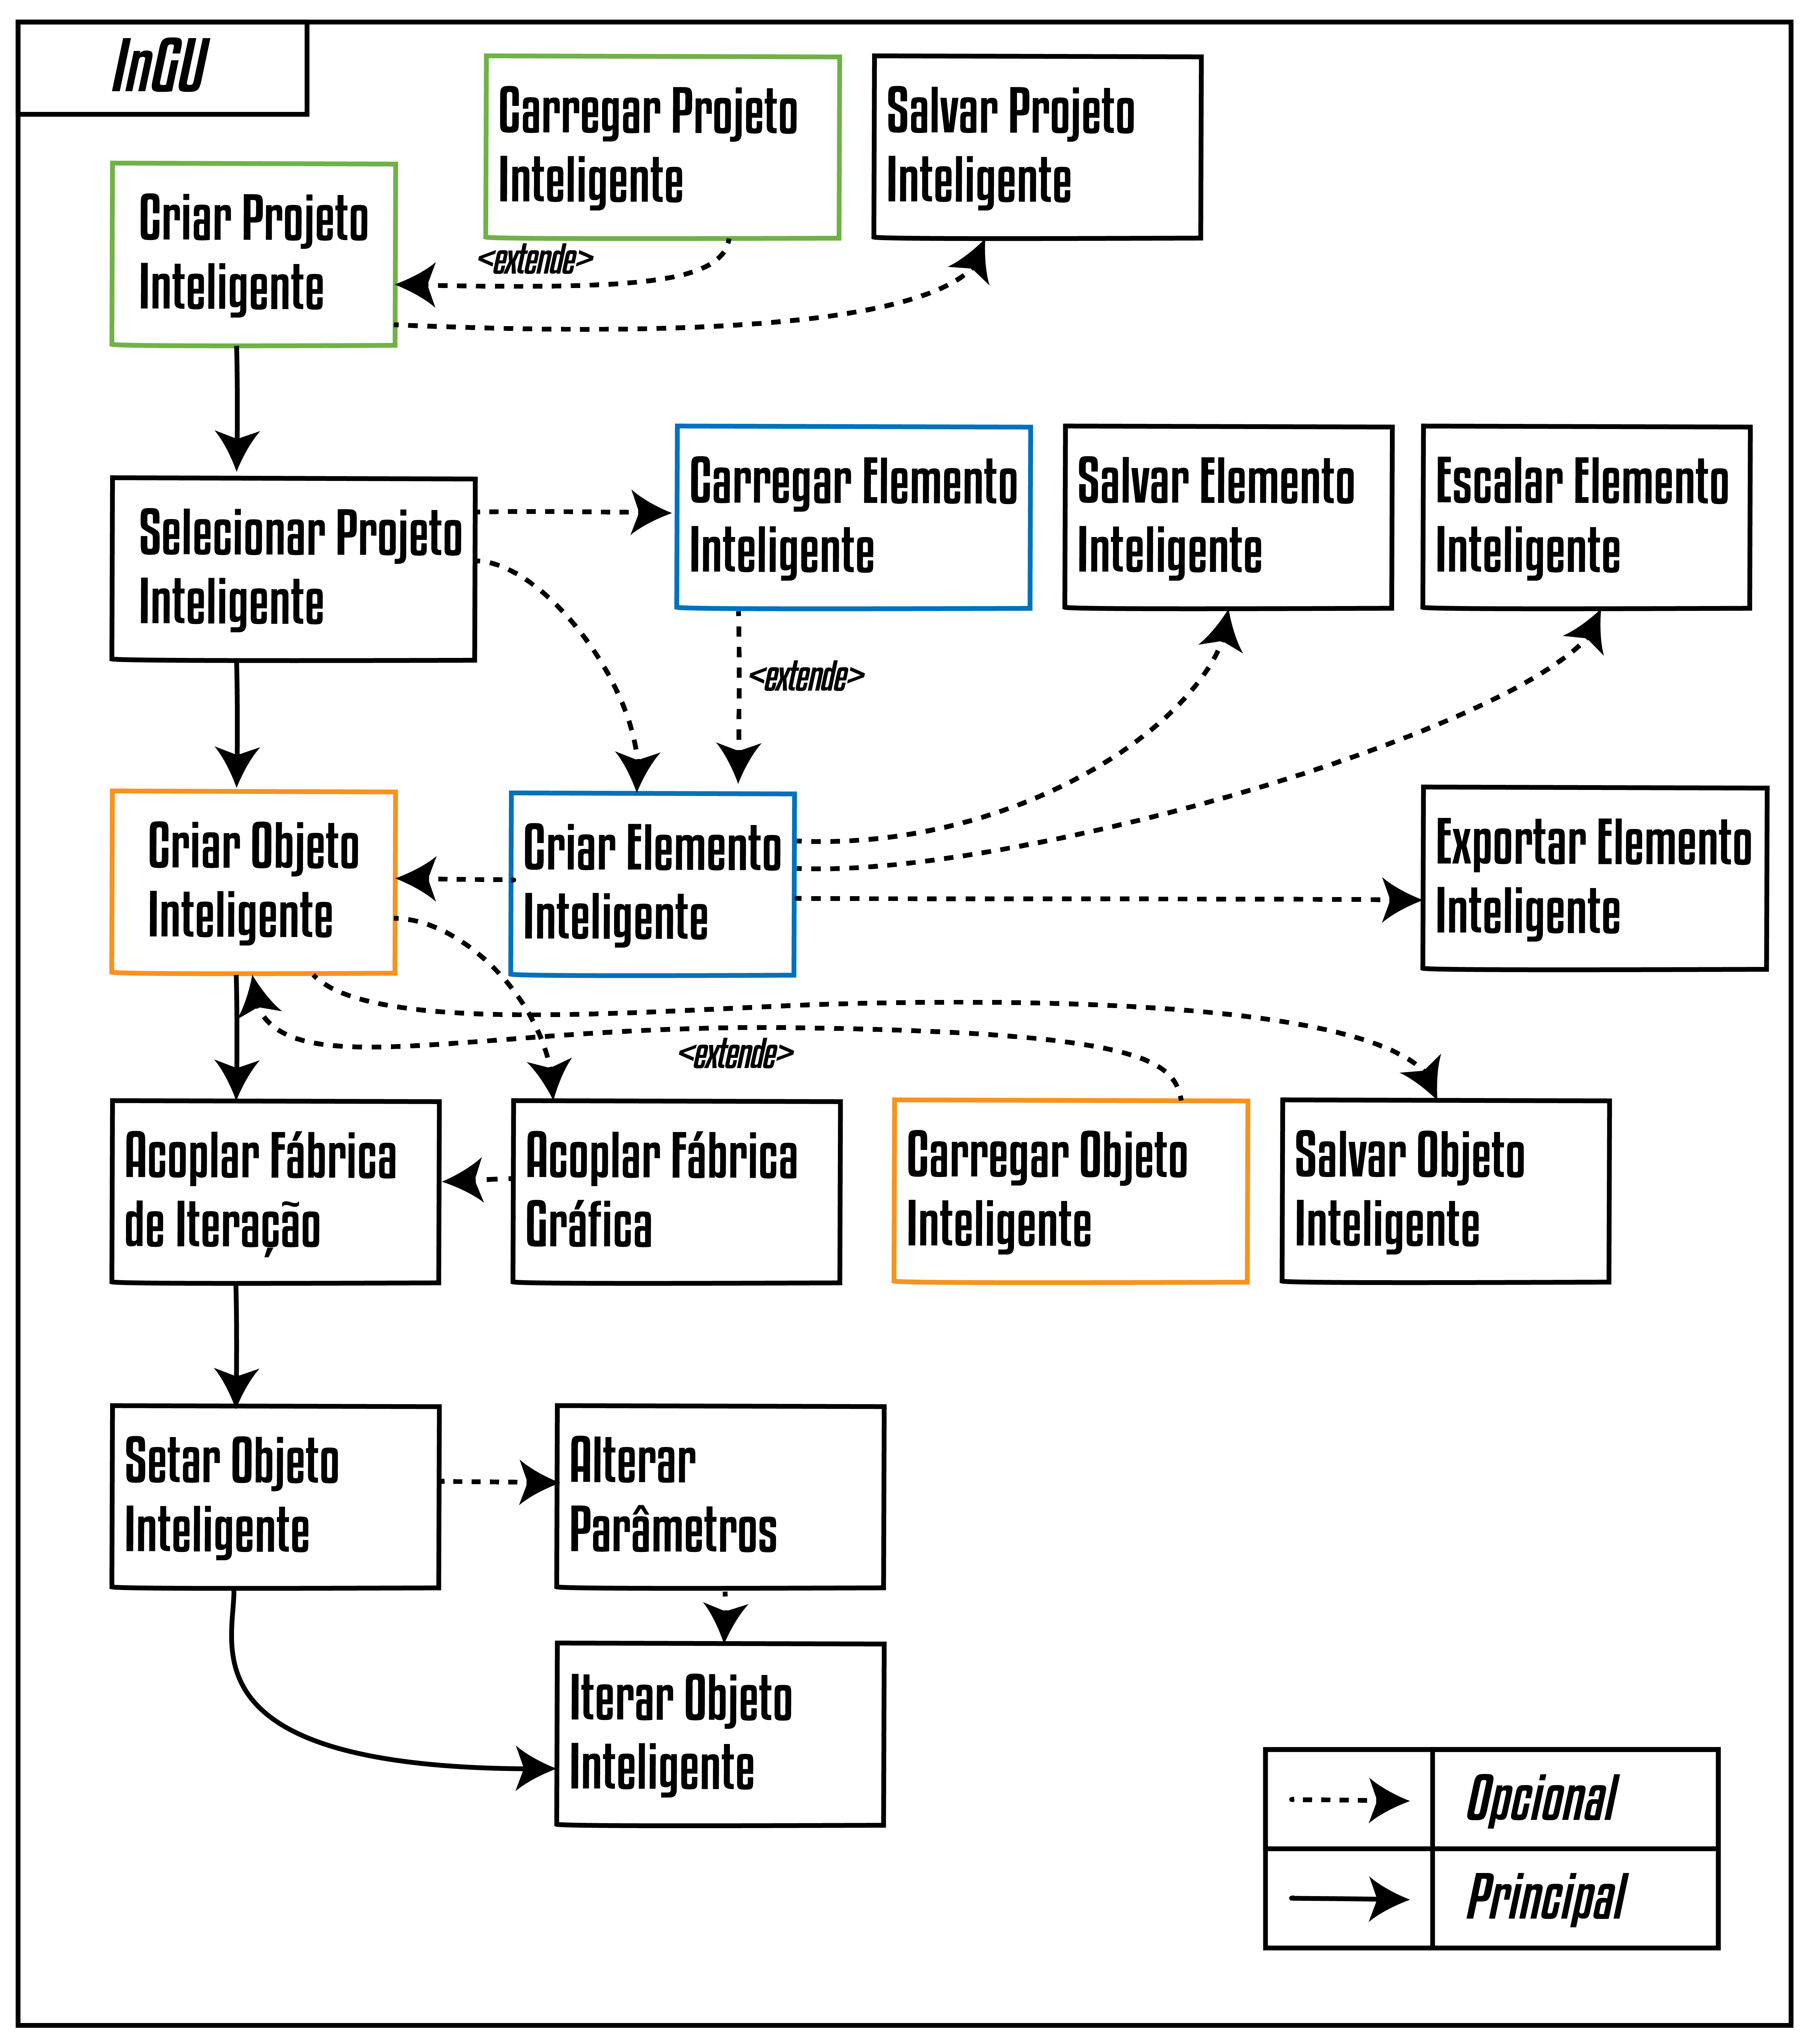
\includegraphics[width=\linewidth]{Figures/CasoDeUso@16x.png}
	\caption{Fluxograma do ambiente computacional InGU, em azul as atividades de criação de elementos inteligentes, em verde as atividades de criação de projetos inteligentes e em laranja as atividades de criação de objetos inteligentes.}
	\label{fig:caso_uso}
\end{figure}

A Figura~\ref{fig:caso_uso} demonstra a principal sequência de atividades executadas para se iterar um objeto inteligente. Como descrito na Seção~\ref{sec:estrutura}, um objeto inteligente recém-criado não pode ser iterado, ele precisa antes ser corretamente configurado. Com este modelo é possível observar a sequência de passos necessárias para se iterar um obejto inteligente.

Primeiramente, é necessário criar um projeto inteligente e selecioná-lo. Cada atividade representada no fluxograma é executada por um comando correspondente, o mesmo fluxo pode ser observado no Anexo~\ref{annex2}. As primeiras linhas de comando representadas neste arquivo de comandos são de criação de projetos.

Ao criar um objeto inteligente, seus elemento inteligentes são juntamente criados, ambas estas funcionalidades estão disponíveis ao usuário uma vez que ele tenha selecionado um projeto. É possível ainda que se cria um objeto inteligente à partir de um elemento inteligente, desta forma é garantida também a igualdade inicial entre os modelos.

Com um objeto criado corretamente é possível adicionar à ele uma fábrica de iteração e uma gráfica. Ao acoplar a fábrica de iteração o método iterativo é liberado, bem como a possibilidade de alterar os parâmetros do objeto inteligente.

Foi adicionada também a possibilidade de se exportar elementos inteligentes, para o caso de alguns elementos inteligentes como \textit{WiseGraphic} isso siginifca a exportação de imagem no formato \textbf{P}ortable \textbf{N}etwork \textbf{G}raphics, ou \textit{png}, com seu comando representado na linha $7$ do Anexo~\ref{annex2}.

Como mencionado anteriormente, a mesma estrutura foi utilizada na construção do ambiente computacional composto por elementos gráficos \textit{IGU}. Desta forma o principal fluxo de uso da interface gráfica foi desenvolvido.

\begin{figure}[!htbp]
	\centering
	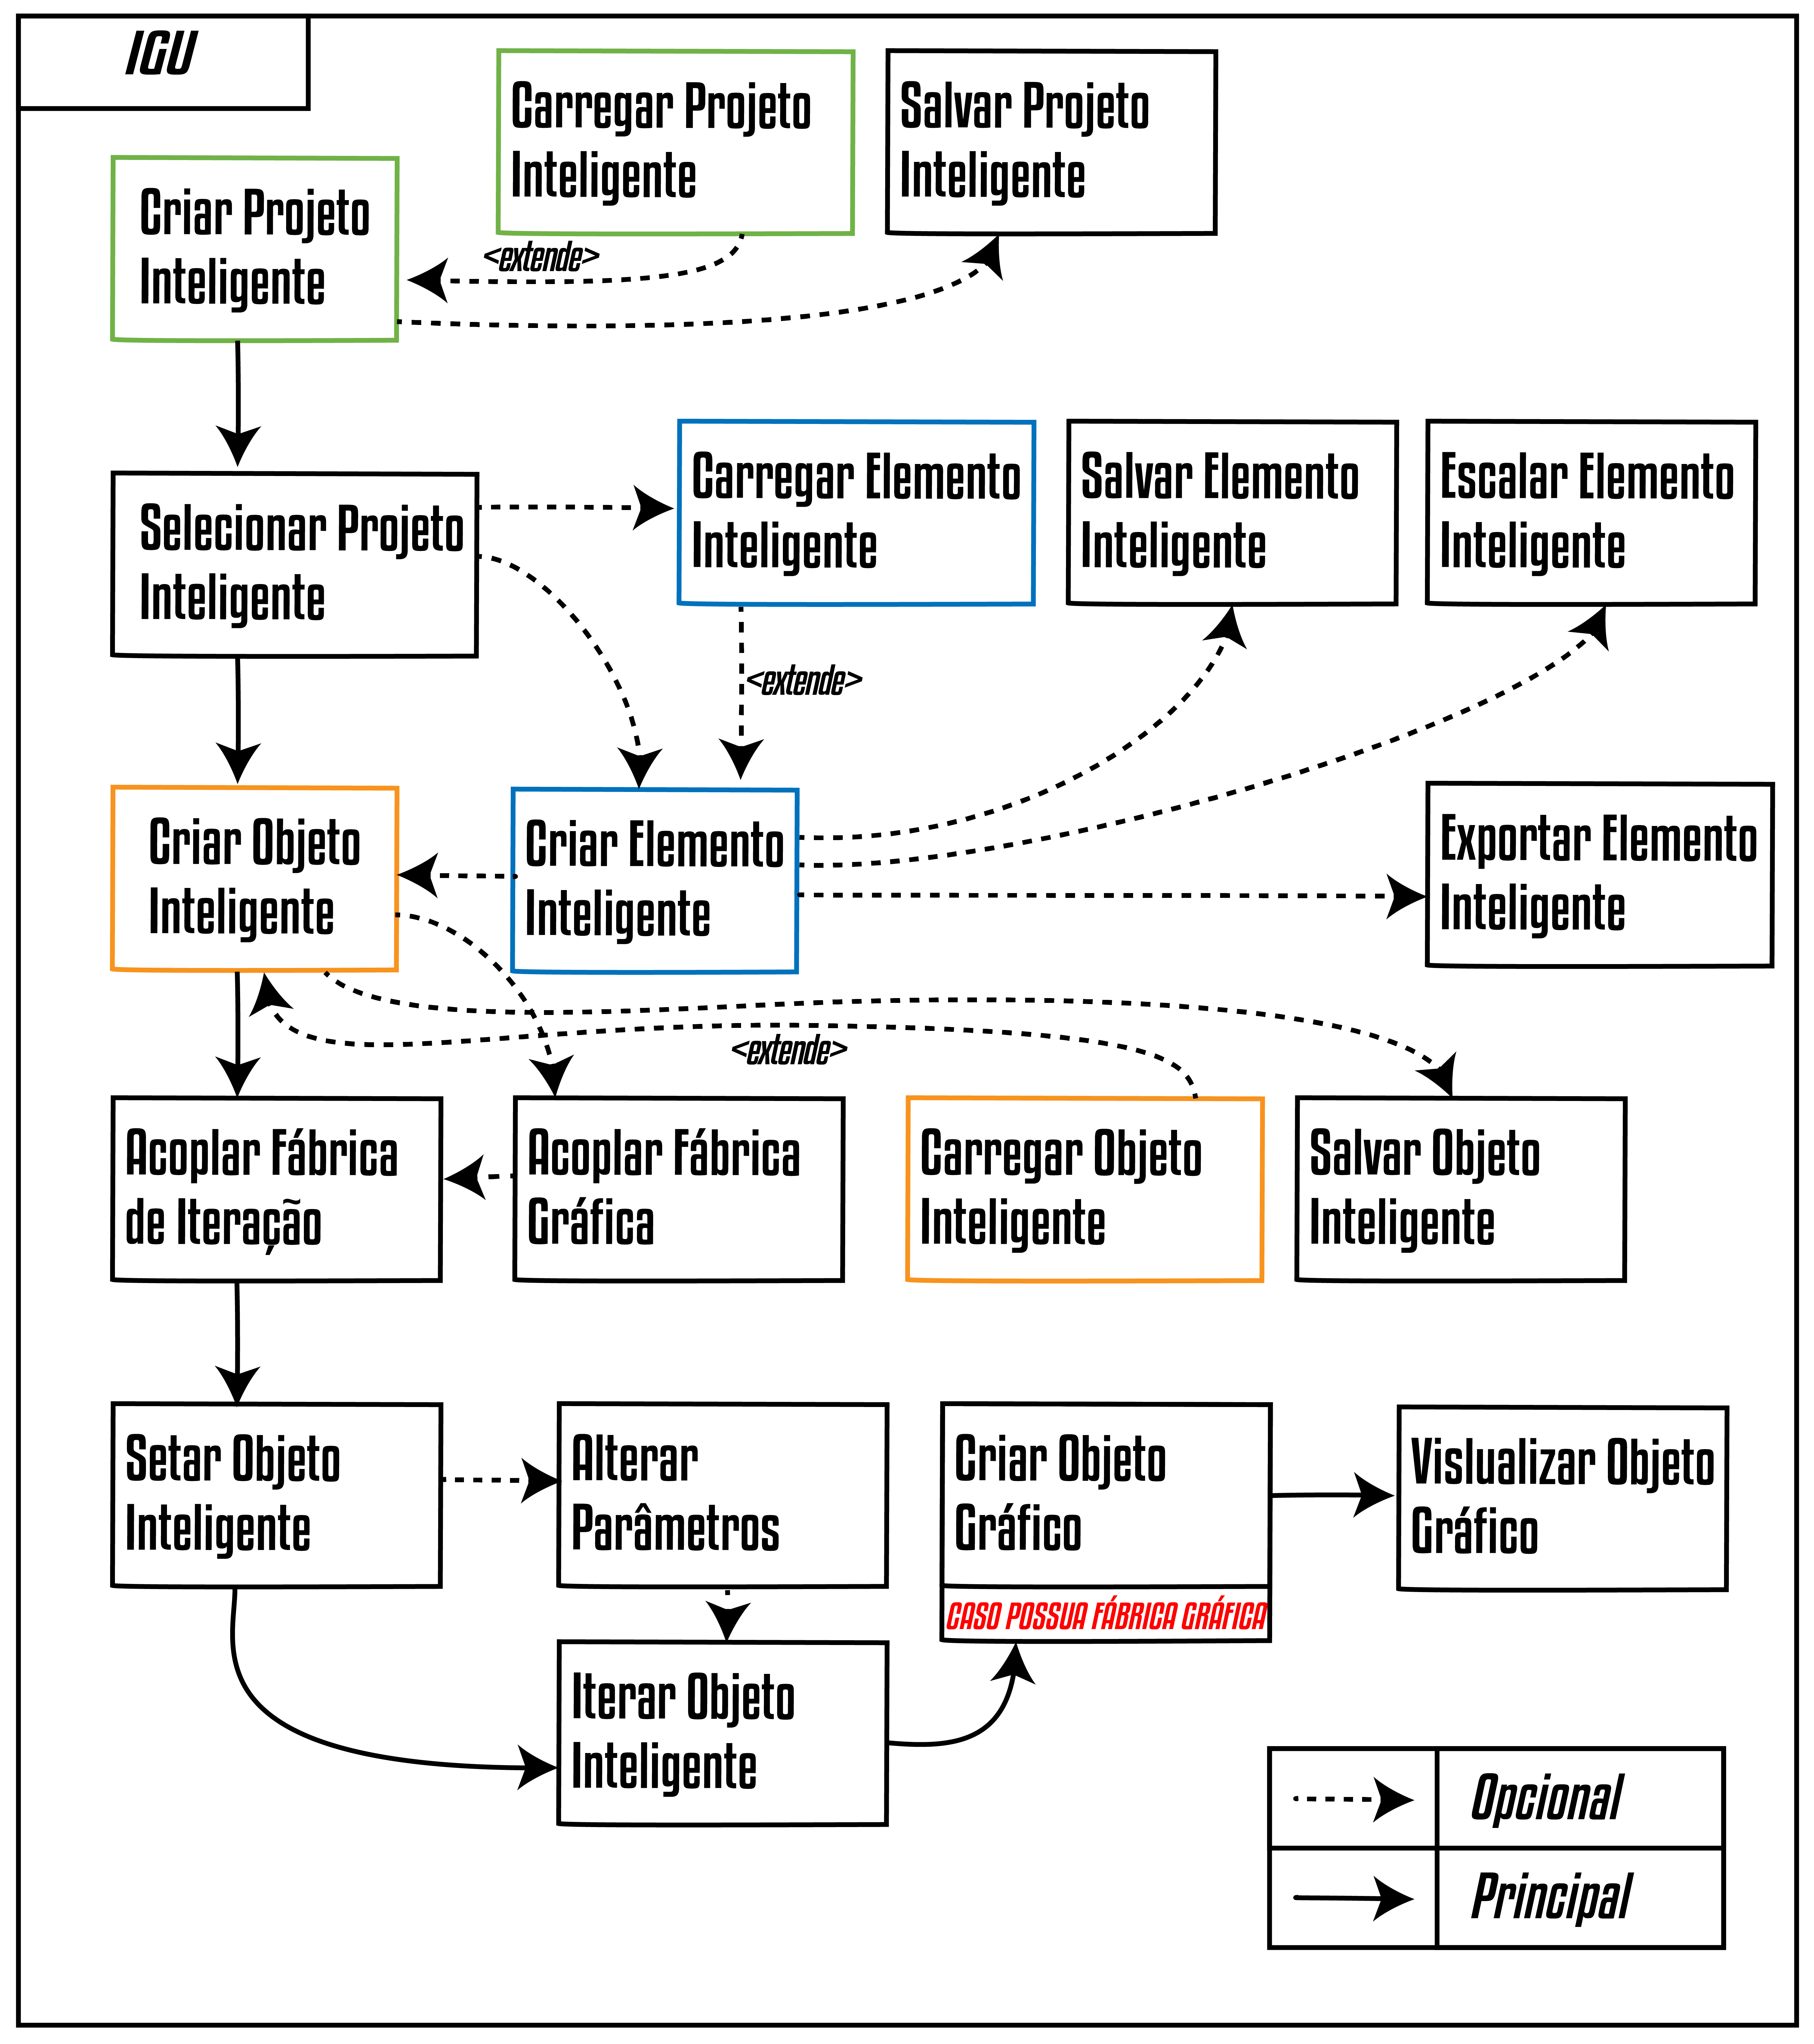
\includegraphics[width=\linewidth]{Figures/CasoDeUso2@16x.png}
	\caption{Fluxo de caso de uso do ambiente computacional IGU.}
	\label{fig:caso_uso2}
\end{figure}

Finalmente, o funcionamento apresentado pela Figura~\ref{fig:caso_uso2} difere do apresentado na Figura~\ref{fig:caso_uso} apenas na visualização dos objetos gráficos disponibilizada pelos elementos gráficos. Isto garante que ambos os ambientes computacionais sejam alterados em uma eventual atualização de código e que tenham funcionamento idêntico.

%--------------------------------------------------------------------------------%
\section{JANELA PRINCIPAL}\label{sec:janela}

O ambiente com interface gráfica foi nomeado de \textbf{I}terador \textbf{G}ráfico \textbf{U}niversal, que também está presente como parte de um projeto \textit{Qt}/\textit{C++}. Diferentemente dos outro ambiente, este possui elementos gráficos. O principal elemento gráfico disponibilizado pela interface gráfico é a janela principal, que é um objeto do tipo \textit{QMainWindow}. Estes objetos são disponibilizados pela biblioteca \textit{Qt} e permitem que um projeto \textit{C++} possua uma interface gráfica utilizando diretivas OpenGL e GLUT (The OpenGL Utility Kit).

Ao abrir o ambiente computacional a tela principal com seus elementos gráficos é exibida.

\begin{figure}[!htbp]
	\centering
	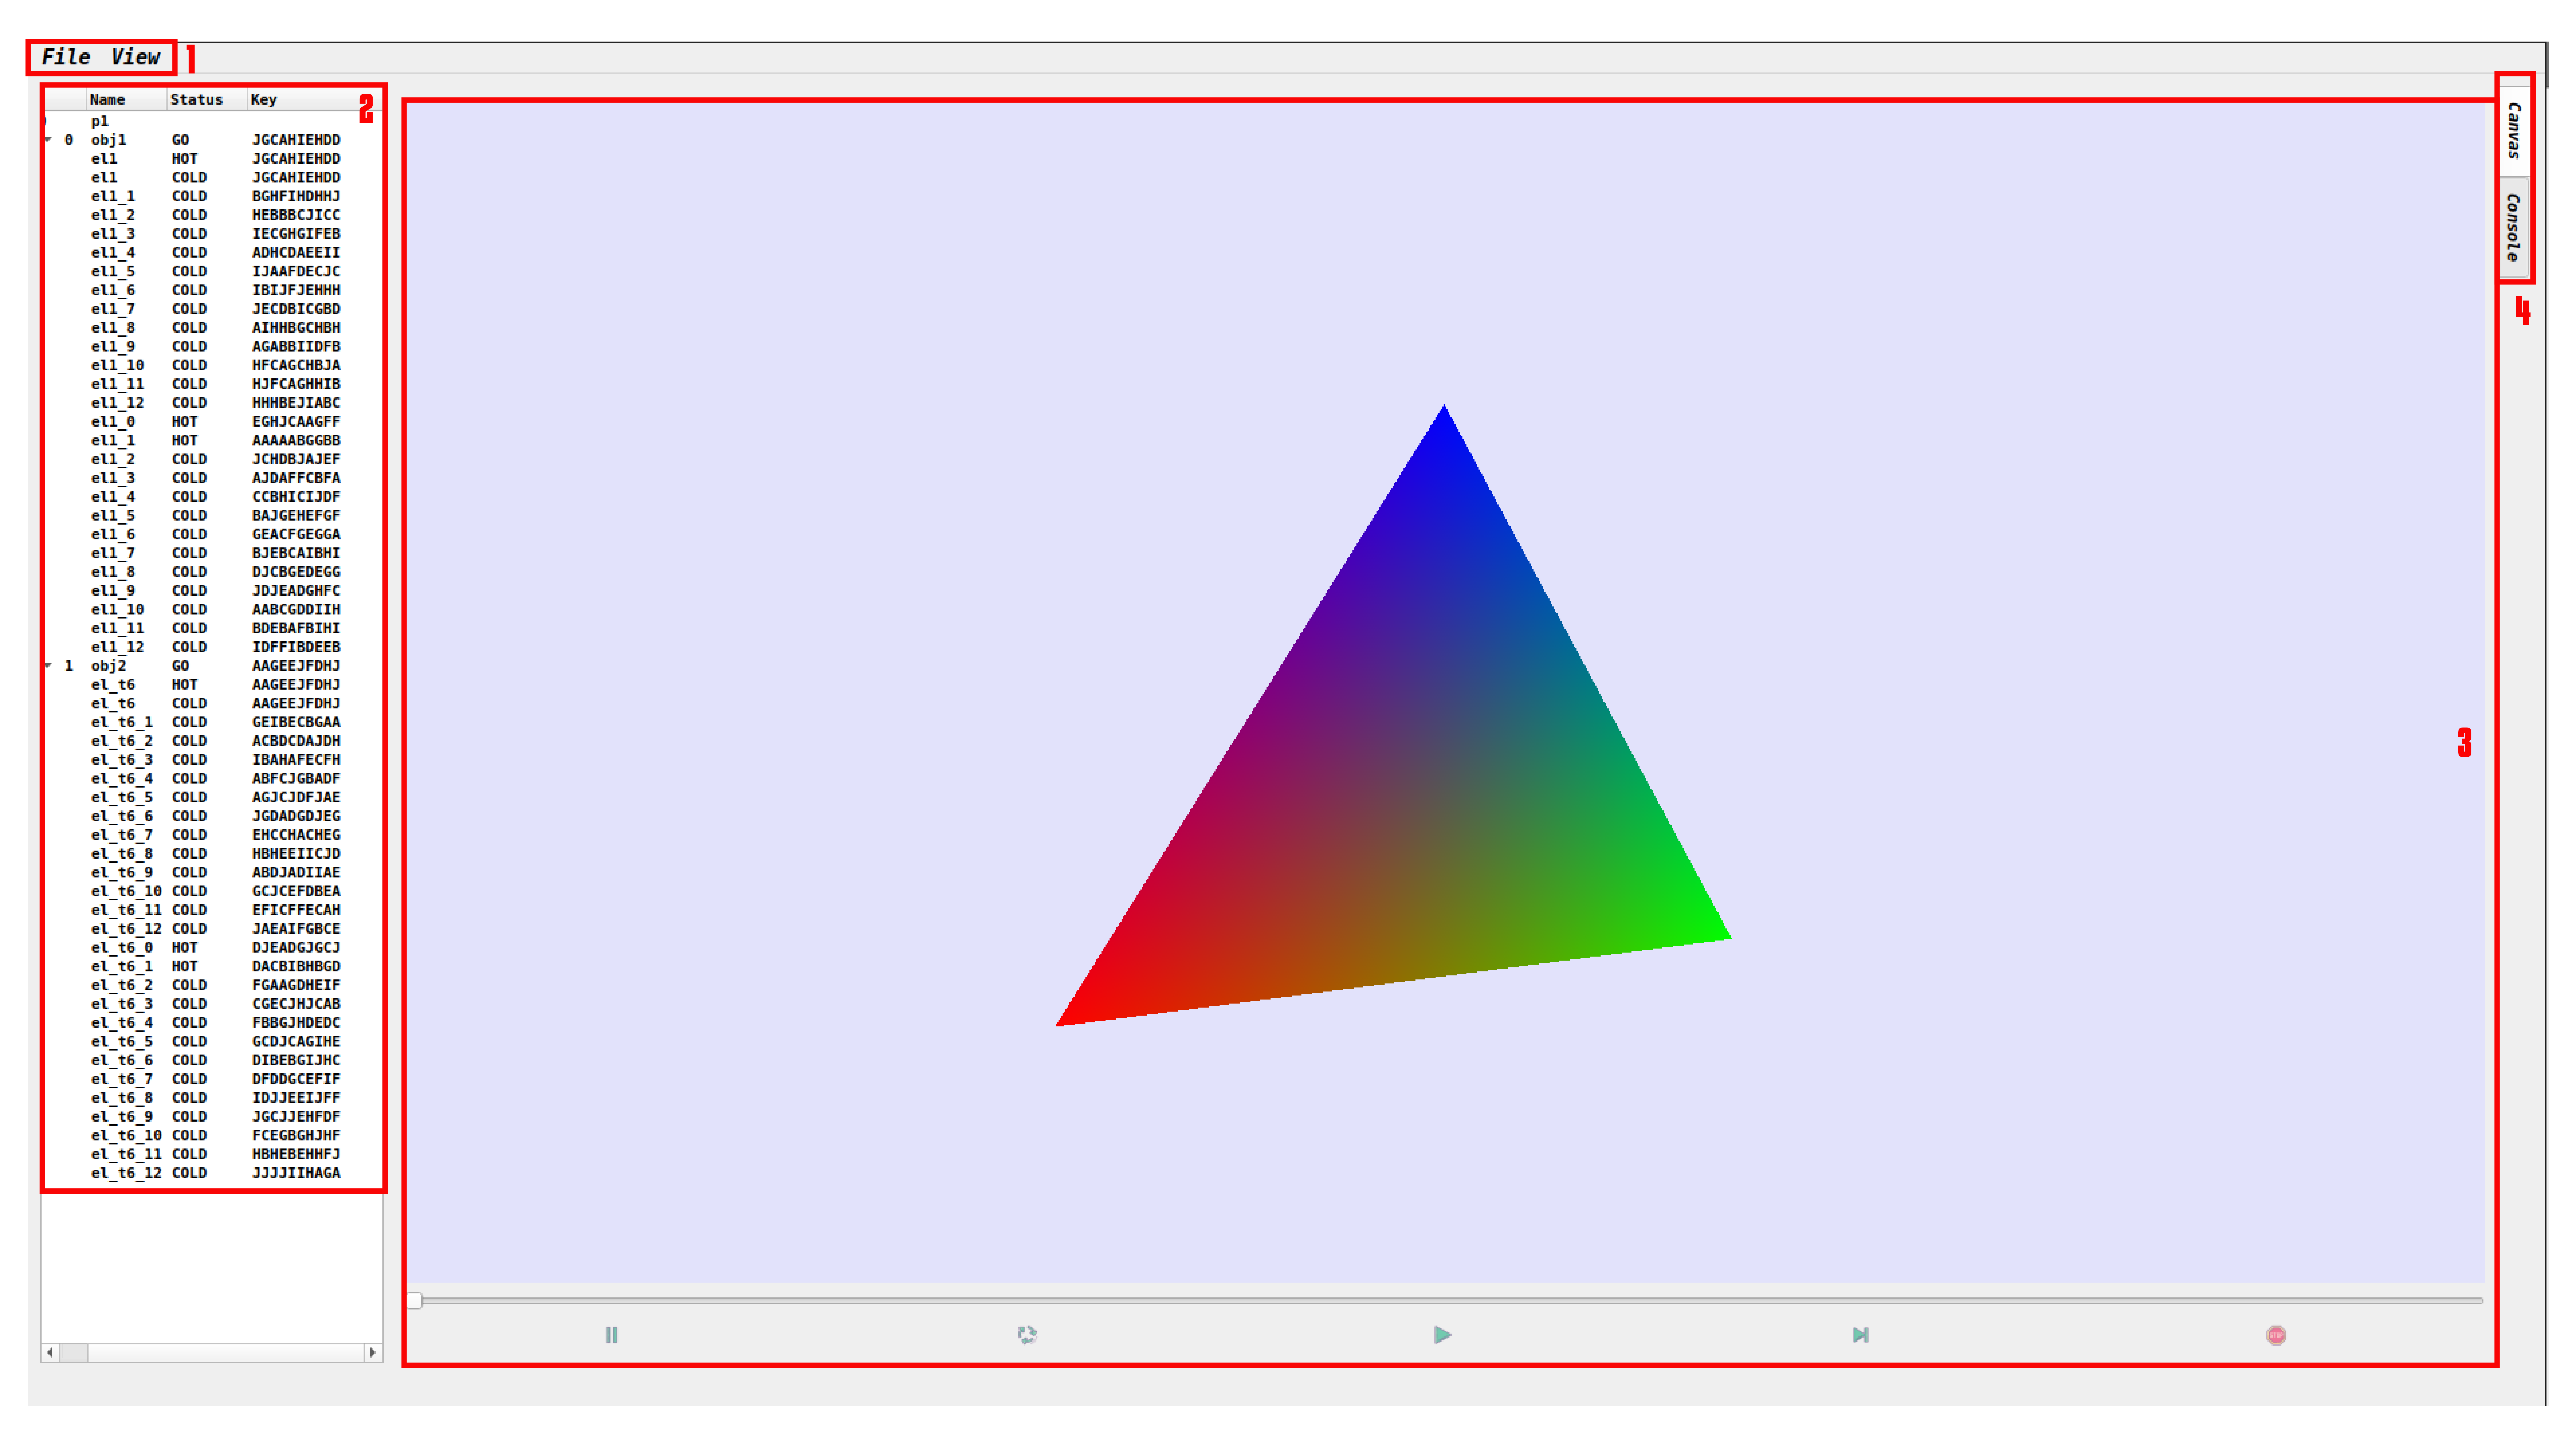
\includegraphics[width=\linewidth]{Figures/IGU_001a.png}
	\caption{Janela principal ambiente computacional IGU. Da esquerda para a direita: 1. Menu principal do programa; 2. Árvore de projetos e seus elementos; 3. Área de trabalho, no caso mostrando OpenGl \textit{Canvas}; 4. Seleção de abas}
	\label{fig:UI}
\end{figure}

A Figura~\ref{fig:UI} demonstra o comportamento inicial da ferramenta computacional. Ao ser aberta o ambiente de trabalho é recuperado, projetos, objetos e elementos são recuperados de um arquivo contido na mesma parta da ferramenta computacional. Este arquivo é salvo toda vez que a ferramenta computacional é encerrada com projetos inteligentes ainda no ambiente. Ainda nesta figura estão representados os principais grupos de elementos gráficos.

As próximas seções discorrem sobre cada grupo de elemento gráfico presente na janela principal da ferramenta computacional e seu funcionamento.

%--------------------------------------------------------------------------------%
\subsection{MENU}\label{sec:menu}

O primeiro grupo são os elementos que compões o menu principal da aplicação. Cada opção do menu é representada por um uma linha de texto, ao selecionar a linha uma ação é executada:

\begin{figure}[!htbp]
	\centering
	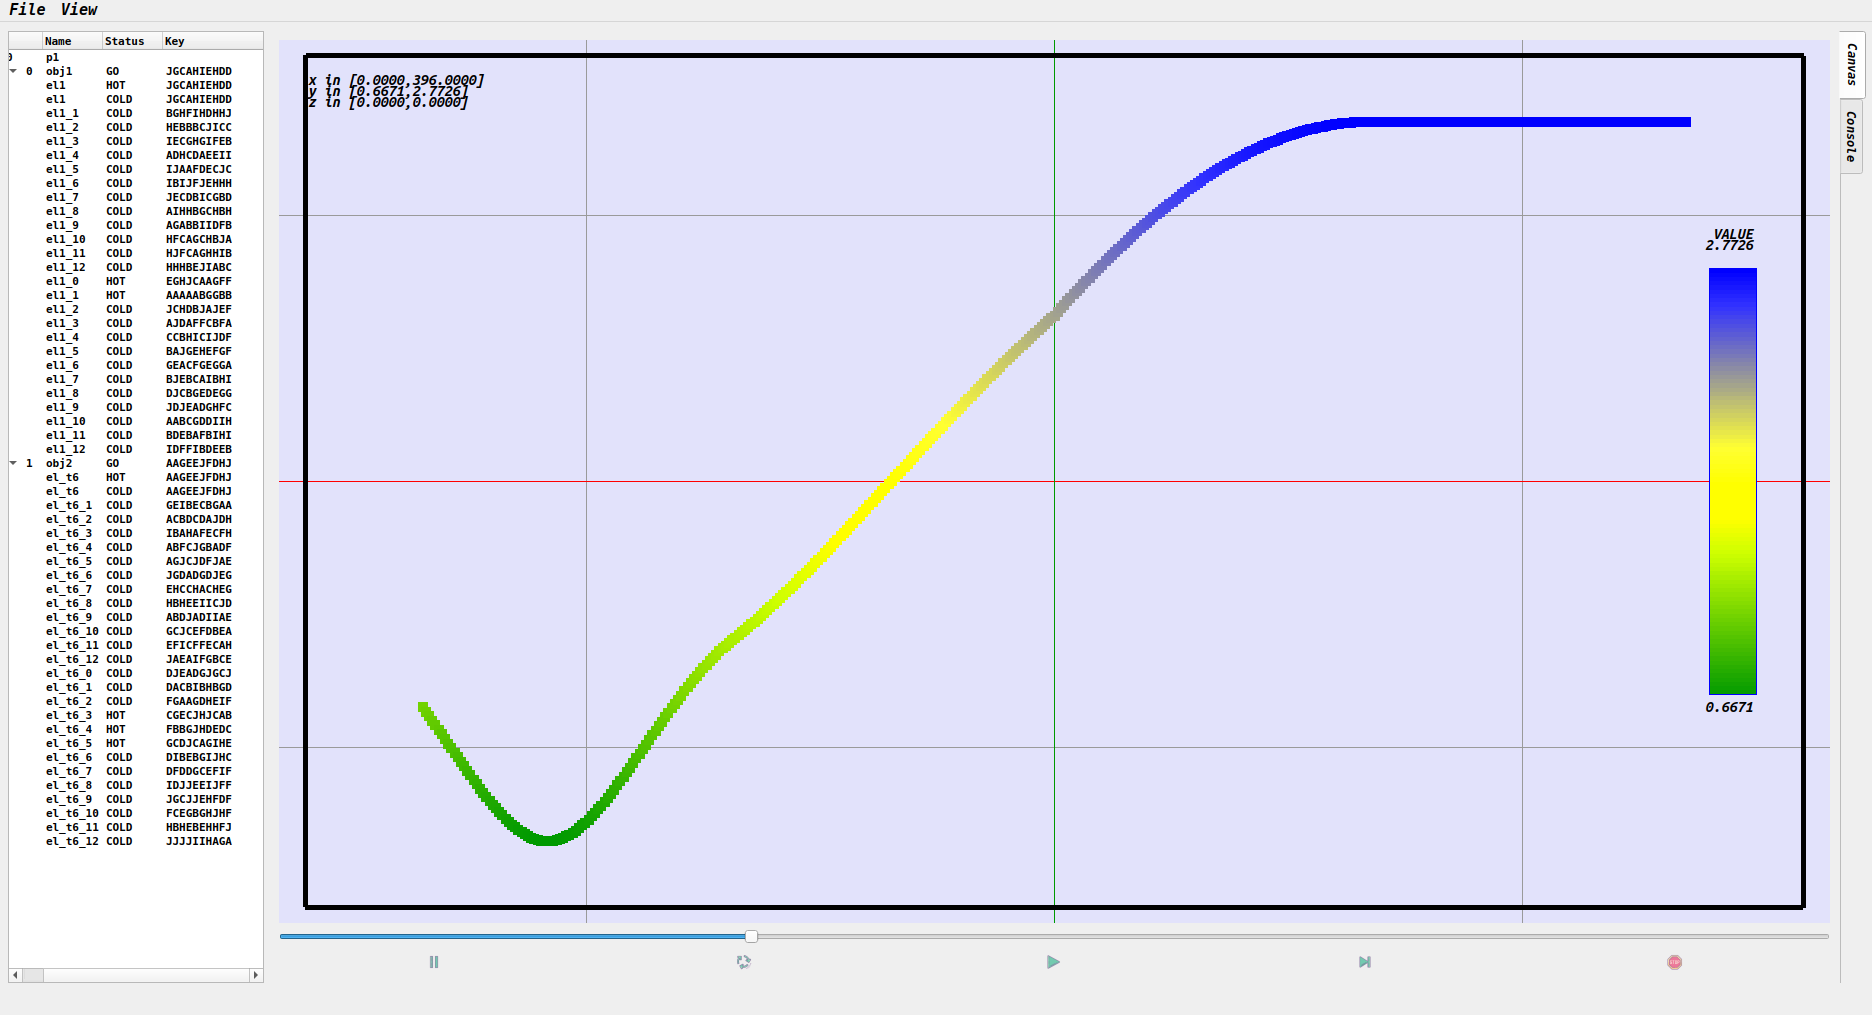
\includegraphics[scale=1]{Figures/IGU_016.png}
	\caption{Opções do menu principal da ferramenta computacional \textit{IGU}}
	\label{fig:menu}
\end{figure}


\begin{itemize}
	\item \textbf{Exit}: Fecha o ambiente computacional.
	\item \textbf{Jobs}: Abre a Janela que exibe os trabalhos inteligentes criados.
	\item \textbf{Open Canvas}: Abre uma nova janela contendo um novo elemento gráfico OpenGL \textit{Canvas}.
\end{itemize}

Ao abrir um novo elemento gráfico \textit{Canvas}, uma nova listagem é exibida ao executar o comando de listar canvas. Isso possibilita que mais de um objeto seja exibido ao mesmo tempo em janelas distintas.

%--------------------------------------------------------------------------------%
\subsection{ABAS \& ÁREA DE TRABALHO}\label{sec:abas}

As abas da janela principal selecionam o elemento de interface gráfica que será exibido na área de trabalho da aplicação.

\begin{figure}[!htbp]
	\centering
	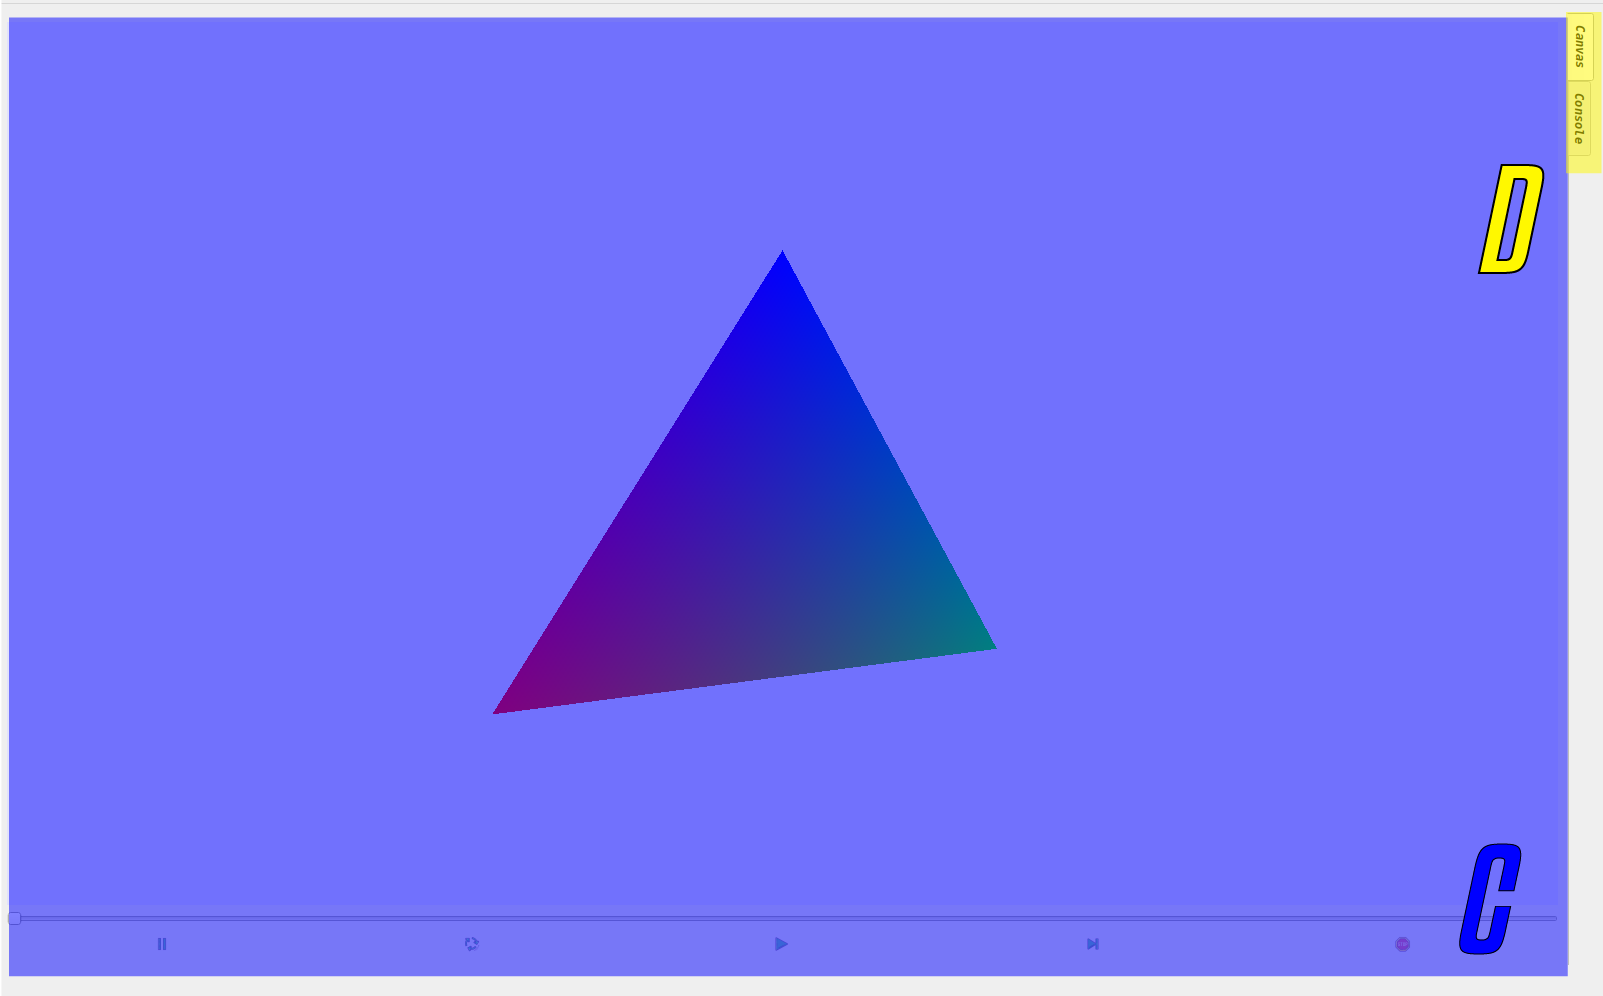
\includegraphics[width=\linewidth]{Figures/IGU_001a_34.png}
	\caption{Opções do menu principal da ferramenta computacional \textit{IGU}}
	\label{fig:abas}
\end{figure}

Ao selecionar uma das abas, os elementos de interface de usuário da área de trabalho são trocados. Estes elementos são objetos do tipo \textit{QWidget}, estes objetos que são divididos em dois ambientes, o \textit{Canvas} e o \textit{Console}. 

Ao selecionar a opção do \textit{Console} um ambiente similar ao disponibilizado pelo ambiente \textit{InGU} é disponibilizado. Utilizando um elemento de exibição textual longa, uma linha de texto como entrada e um botão, os mesmo comandos disponibilizados na Seção~\ref{sec:console} são acessados por estes elementos gráficos. Para executar uma linha de comando basta inserir-la no elemento gráfico e pressionar o botão ou a tecla \textit{Enter}, a resposta será acoplada ao elemento de exibição textual longa.

\begin{figure}
	\centering
	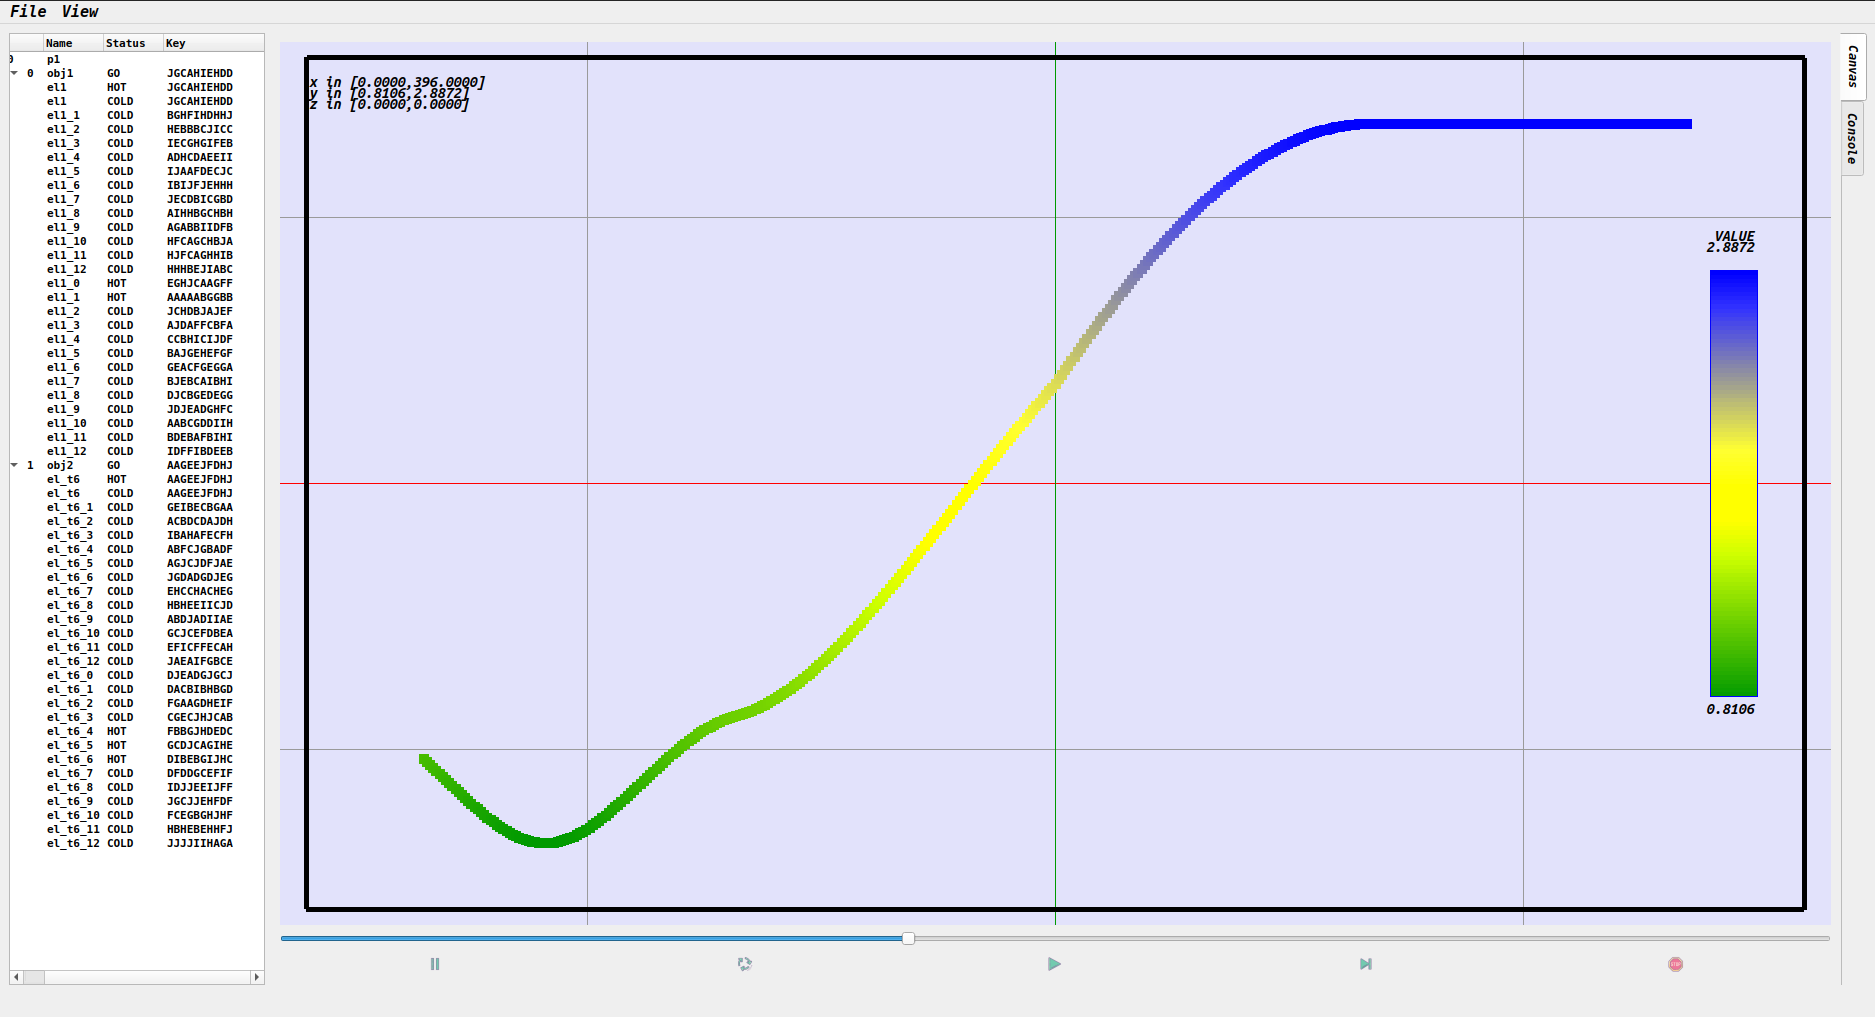
\includegraphics[width=.9\linewidth]{Figures/IGU_017.png}
	\caption{Mudanças gráficas observadas na Área de Trabalho ao trocar a aba selecionada, exibindo o elemento gráfico \textit{Canvas} com a aba \textit{Canvas} selecionada.}
	\label{fig:sfig1}
\end{figure}

\begin{figure}
	\centering
	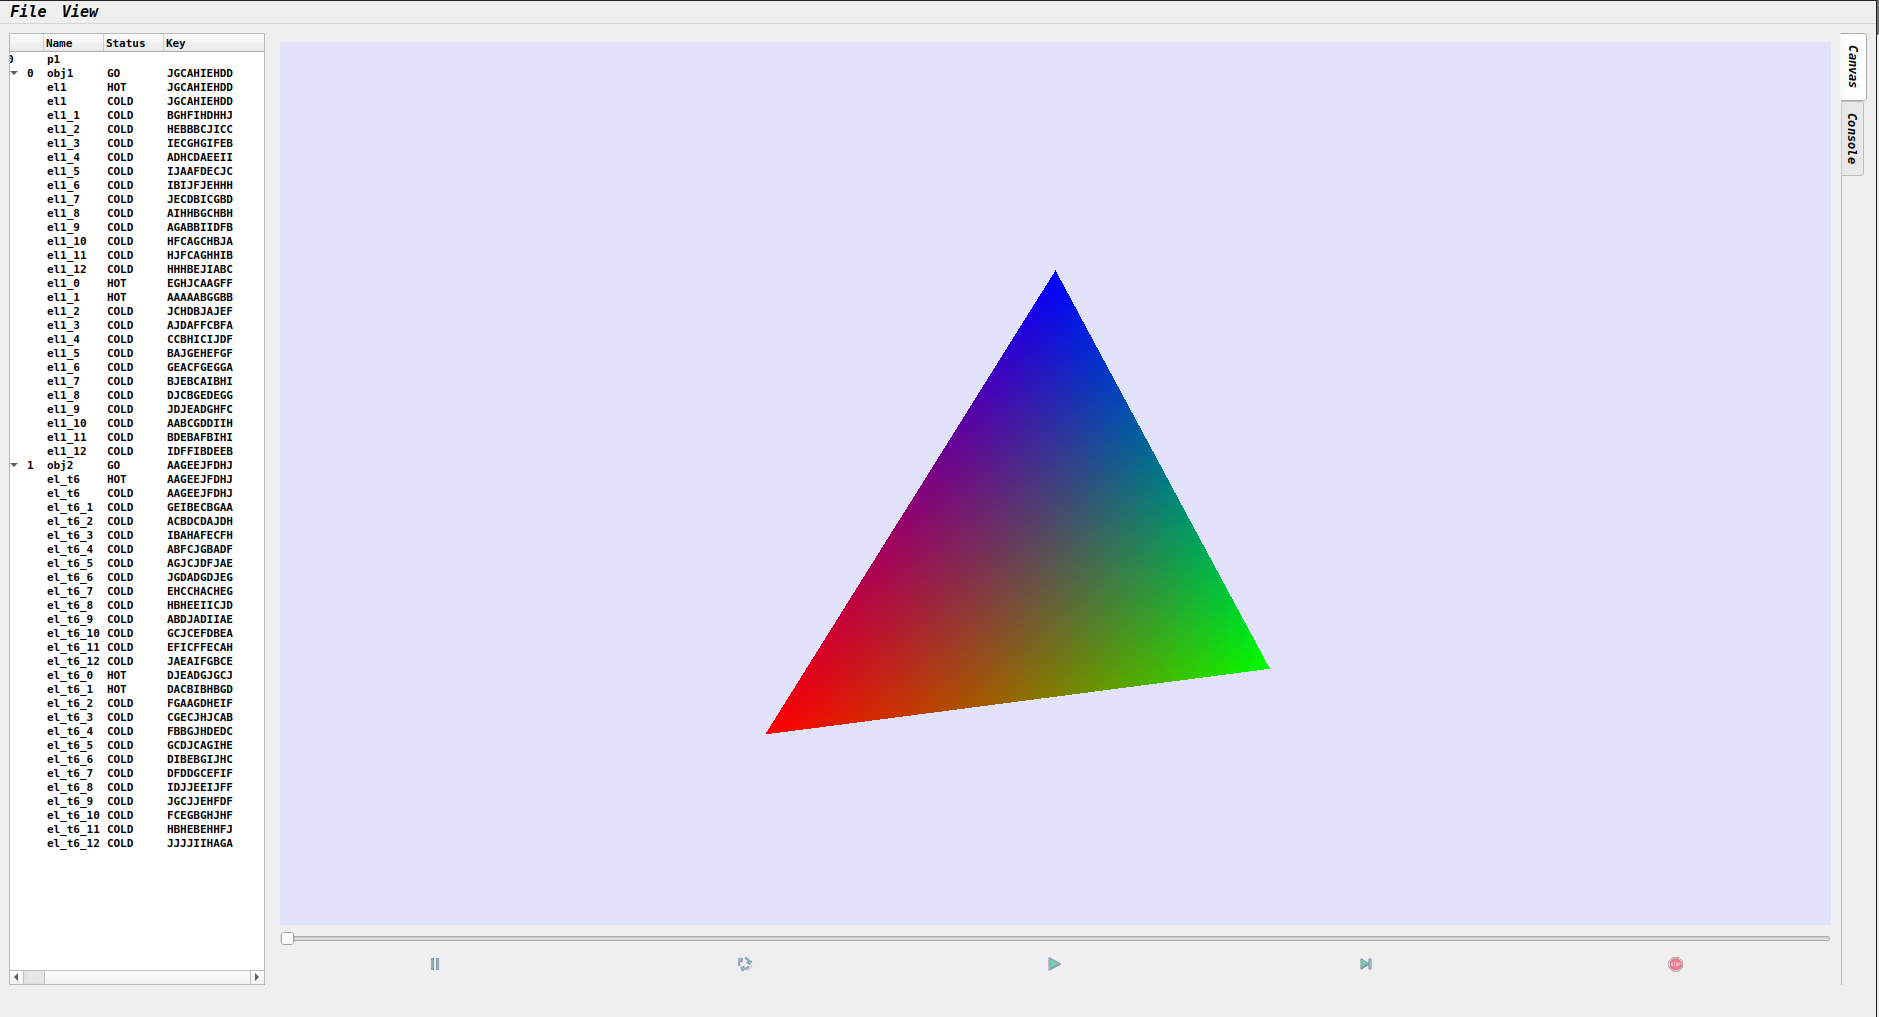
\includegraphics[width=.9\linewidth]{Figures/IGU_001.png}
	\caption{Mudanças gráficas observadas na Área de Trabalho ao trocar a aba selecionada, exibindo o elemento gráfico \textit{Console} com a aba \textit{Console} selecionada.}
	\label{fig:sfig2}
\end{figure}

A Figura~\ref{fig:fig} mostra as áreas de trabalho disponibilizadas ao selecionar uma das abas. Através da opção \textit{Canvas}, o elemento gráfico que contém um \textit{QWidget} cuja principal função é uma tela \textit{OpenGL}. Os objetos gráficos, resultados de iterações podem ser visualizados aqui. O funcionamento desta área de trabalho é descrito pela janela \textit{Canvas} e funciona como um 
reprodutor de vídeo.

As abas foram construídas para realizar todas as funções da ferramenta computacional com seus elementos gráficos. O ciclo de vida da thread \textit{WiseThreadPool} esta diretamente ligado À interface gráfica. Ao utilizar a interface gráfica para percorrer os elementos gráficos, ou executar a animação, irão desencadear chamadas diretas as threads disponibilizadas.

%--------------------------------------------------------------------------------%
\section{ÁRVORE DE PROJETOS}\label{sec:arvore_projetos}

Além da área de trabalho, o elemento gráfico que exibe a árvore de projetos se permanece fixa. Este elemento gráfico é um explorador de árvore \textit{QTreeWidget} que exibe todos os projetos carregados e suas estruturas. Esta árvore permite rapidamente verificar os elementos criados, seus nomes, suas chaves únicas e seu status atual.

\begin{figure}[!htbp]
	\centering
	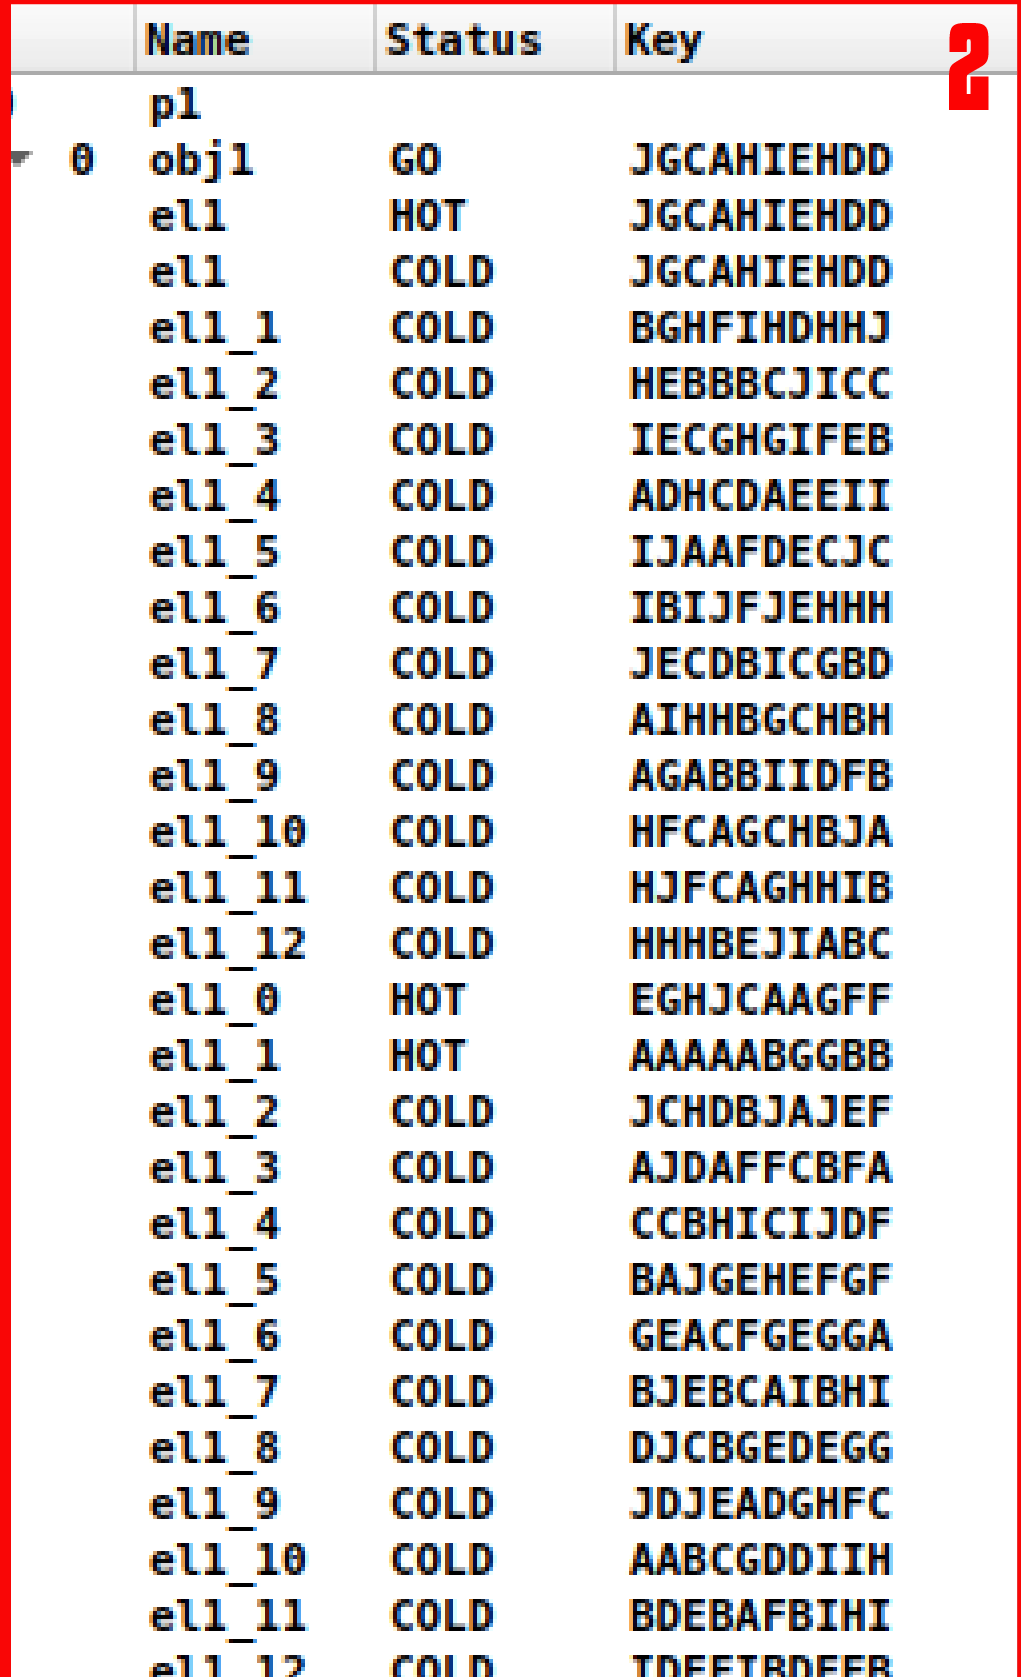
\includegraphics[width=0.4\linewidth]{Figures/IGU_001c.png}
	\caption{Árvore de projetos, na imagem a ferramenta apresenta um projeto inteligente $p1$, um objeto inteligente $obj1$ e seus elementos gráficos e inteligentes.}
	\label{fig:arvores}
\end{figure}

A Figura~\ref{fig:arvores} apresenta o elemento gráfico de uma árvore de projetos com objetos carregados. Na imagem está um projeto nomeado \textit{p1}, um objeto inteligente \textit{obj1} e diversos elementos inteligentes e gráficos. Como visto anteriormente quando o objeto está no estado \textit{GO} significa que ele já foi corretamente configurado e iterado. Dentro deste objeto inteligente estão os elementos inteligentes e gráficos. O primeiro elemento \textit{el1} é o elemento contido na estrutura \textit{Forno} e é o único elemento inteligente no estado \textit{Hot}. Em seguida estão os elementos inteligentes da estrutura \textit{Freezer}, seguidos pelos objetos gráficos.

Através da árvore de projetos é possível observar a troca de estado dos elementos, por exemplo, ao executar a animação os elementos gráficos serão sucessivamente aquecidos. Se observa que a mesma quantidade de elementos gráficos e inteligentes, mantendo a consistência do objeto inteligente, cada passo iterativo com sua respectiva representação gráfica.

%--------------------------------------------------------------------------------%
\section{JANELAS}\label{sec:janelas}

Nesta seção as janelas disponíveis no menu, descrito na Seção~\ref{sec:menu}, são exibidas e seu funcionamento descrito. Existem dois tipos de janelas disponibilizadas pela ferramenta computacional: \textit{Canvas}, que funciona como um reprodutor de vídeo, exibindo elementos gráficos sucessivamente; \textit{Jobs}, exibe todas as demandas criadas pelo programa enviadas à thread inteligente \textit{WiseThreadTool}. Esta última janela pode ser intstanciada apenas uma vez, enquanto diversos \textit{Canvas} podem ser disponibilizados e exibir diferentes objetos.

%--------------------------------------------------------------------------------%
\subsection{JANELA CANVAS}\label{sec:janela_canvas}

A janela e área de trabalho \textit{Canvas} possibilita que o usuário selecione o quadro à ser exibido. Cada quadro representa um objeto do tipo \textit{GraphicObject} que é um componente do modelo gráfico \textit{GraphicModel}. O quadro é selecionado através de uma barra de progresso, além de botões que alteram a animação feita com o objeto gráfico. Estes botões são:

\begin{itemize}
	\item \textbf{Pause}: Pausa a animação do objeto gráfico.
	\item \textbf{Repeat}: Este botão tem um funcionamento liga e desliga, ao ser ligado, quando a animação chegar ao último elemento gráfico retornará ao primeiro.
	\item \textbf{Play}:Este botão também tem um funcionamento liga e desliga, ao ser ligado, o elemento gráfico irá percorrer por todos os quadros da animação.
	\item \textbf{Avançar quadro}: Avança um quadro da animação.
	\item \textbf{Stop}: Caso o \textit{Play} esteja ativo ele é desativado e a tela volta ao primeiro elemento gráfico da animação.
\end{itemize}

Todas as funções do \textit{Canvas} só são disponibilizadas ao usuário depois que um objeto gráfico é ligado à tela \textit{OpenGl}. Neste cenário, quando cada quadro é selecionado é alterado quais objetos gráficos \textit{GraphicObject} estarão no estado aquecido \textit{Hot}. Isto foi feito utilizando a conexão entre objetos \textit{QObjects} e os elementos gráficos \textit{QWidget},desta forma a tela é capaz de acionar diretamente a estrutura do \textit{WiseThreadPool} e selecionar quais elementos debem ser aquecidos e exibidos. A mesma conexão é responsável por enviar a linha de comando da aba \textit{Console} à \textit{WiseThreadPool} para que seja executada e em seguida enviar a mensagem de resposta ao elemento textual.

\begin{figure}[!htbp]
	\centering
	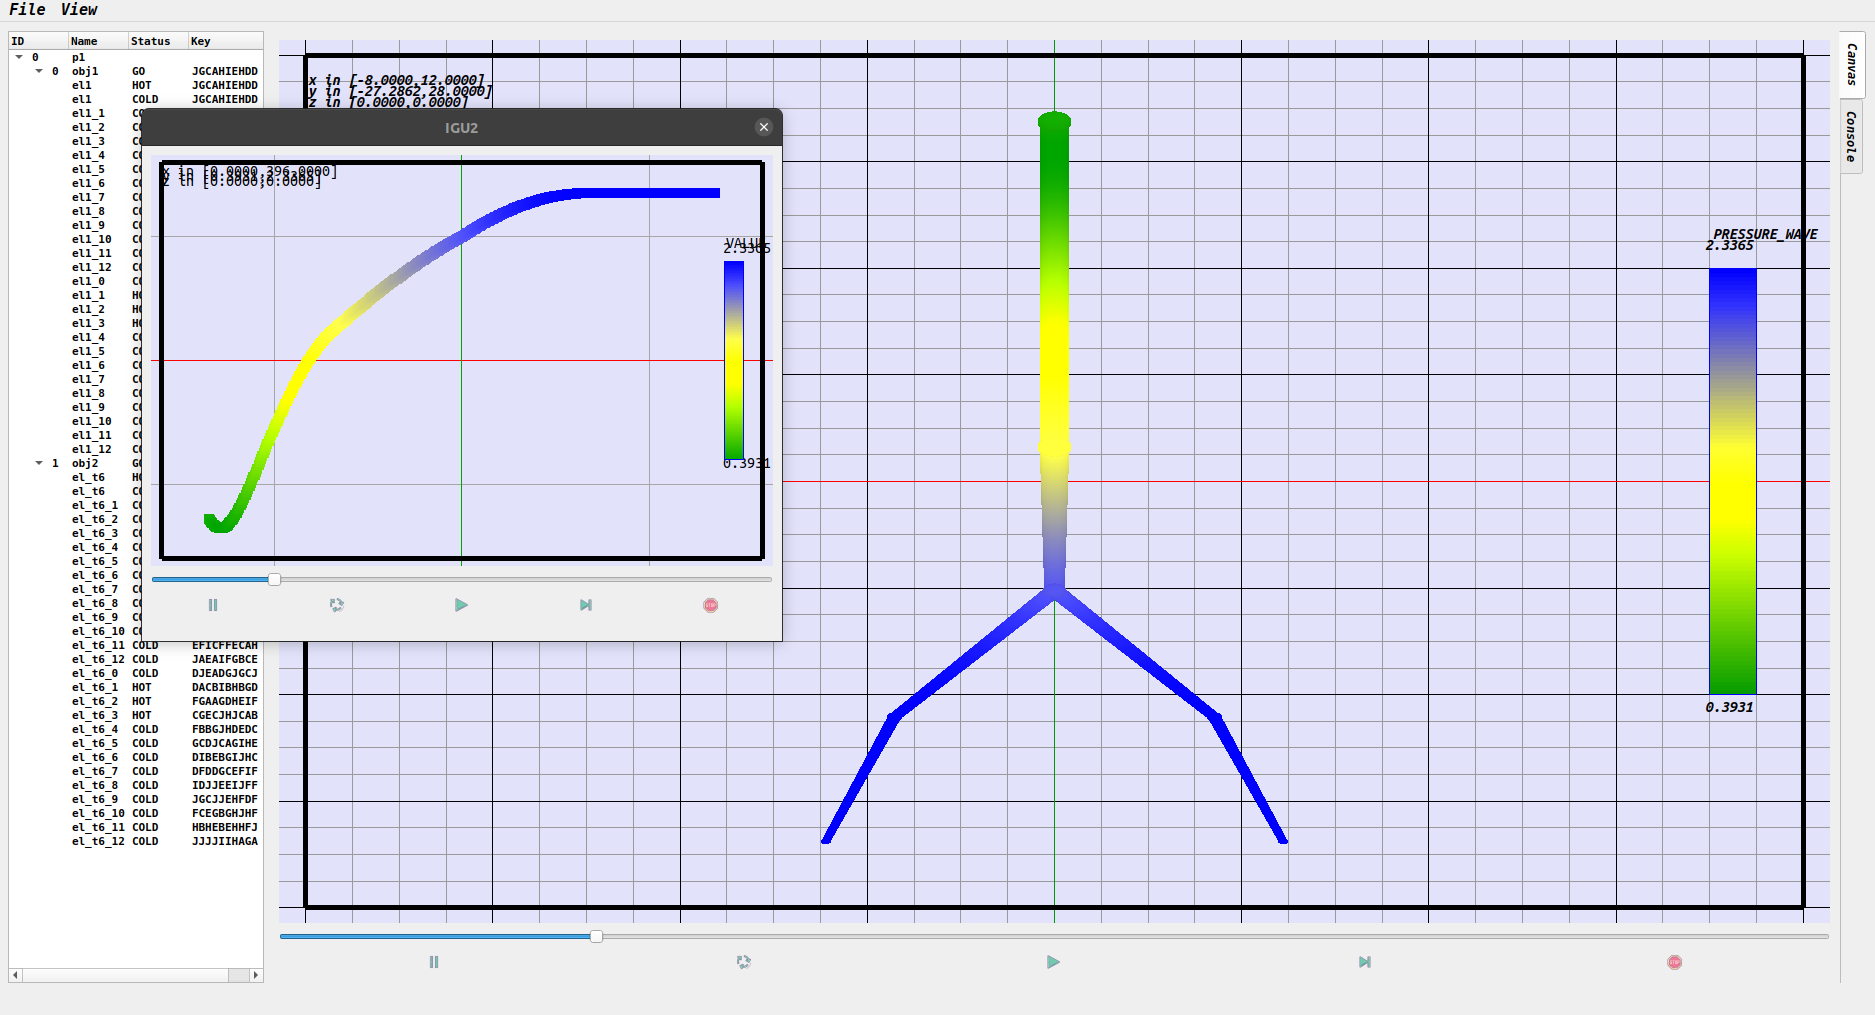
\includegraphics[width=\linewidth]{Figures/IGU_025.png}
	\caption{Janela \textit{Canvas} exibida sobre a área de trabalho \textit{Canvas}, a janela exibindo um gráfico obtido como resultado e a área de trabalho exibindo a árvore arterial estudada.}
	\label{fig:canvas}
\end{figure}

Durante sua execução esta janela irá selecionar o elemento gráfico \textit{GraphicElement} que deve ser exibido, selecionando o elemento através do objeto gráfico \textit{GraphicObject}. Para que o elemento seja exibido corretamente ele precisa estar no estado \textit{Hot}, que representa o momento em que o elemento está corretamente carregado em memória com o modelo geométrico e o parâmetro à ser exibido. Portanto, ao selecionar o elemento à ser exibido o \textit{Canvas} irá criar trabalhos de aquecimento de elementos. A coleção de objetos gráficos \textit{GraphicModel} é encarregada de enviar estes trabalhos a thread inteligente \textit{WiseThreadPool}.

%--------------------------------------------------------------------------------%
\subsection{JANELA JOBS}\label{sec:janela_jobs}

A janela \textit{Jobs} exibe uma listagem compreensiva dos processos inciados e enviados à thread inteligente \textit{WiseThreadPool}, cada comando executado via \textit{Console} ou elemento de interface gráfica irá gerar processos listados nesta janela.

\begin{figure}[!htbp]
	\centering
	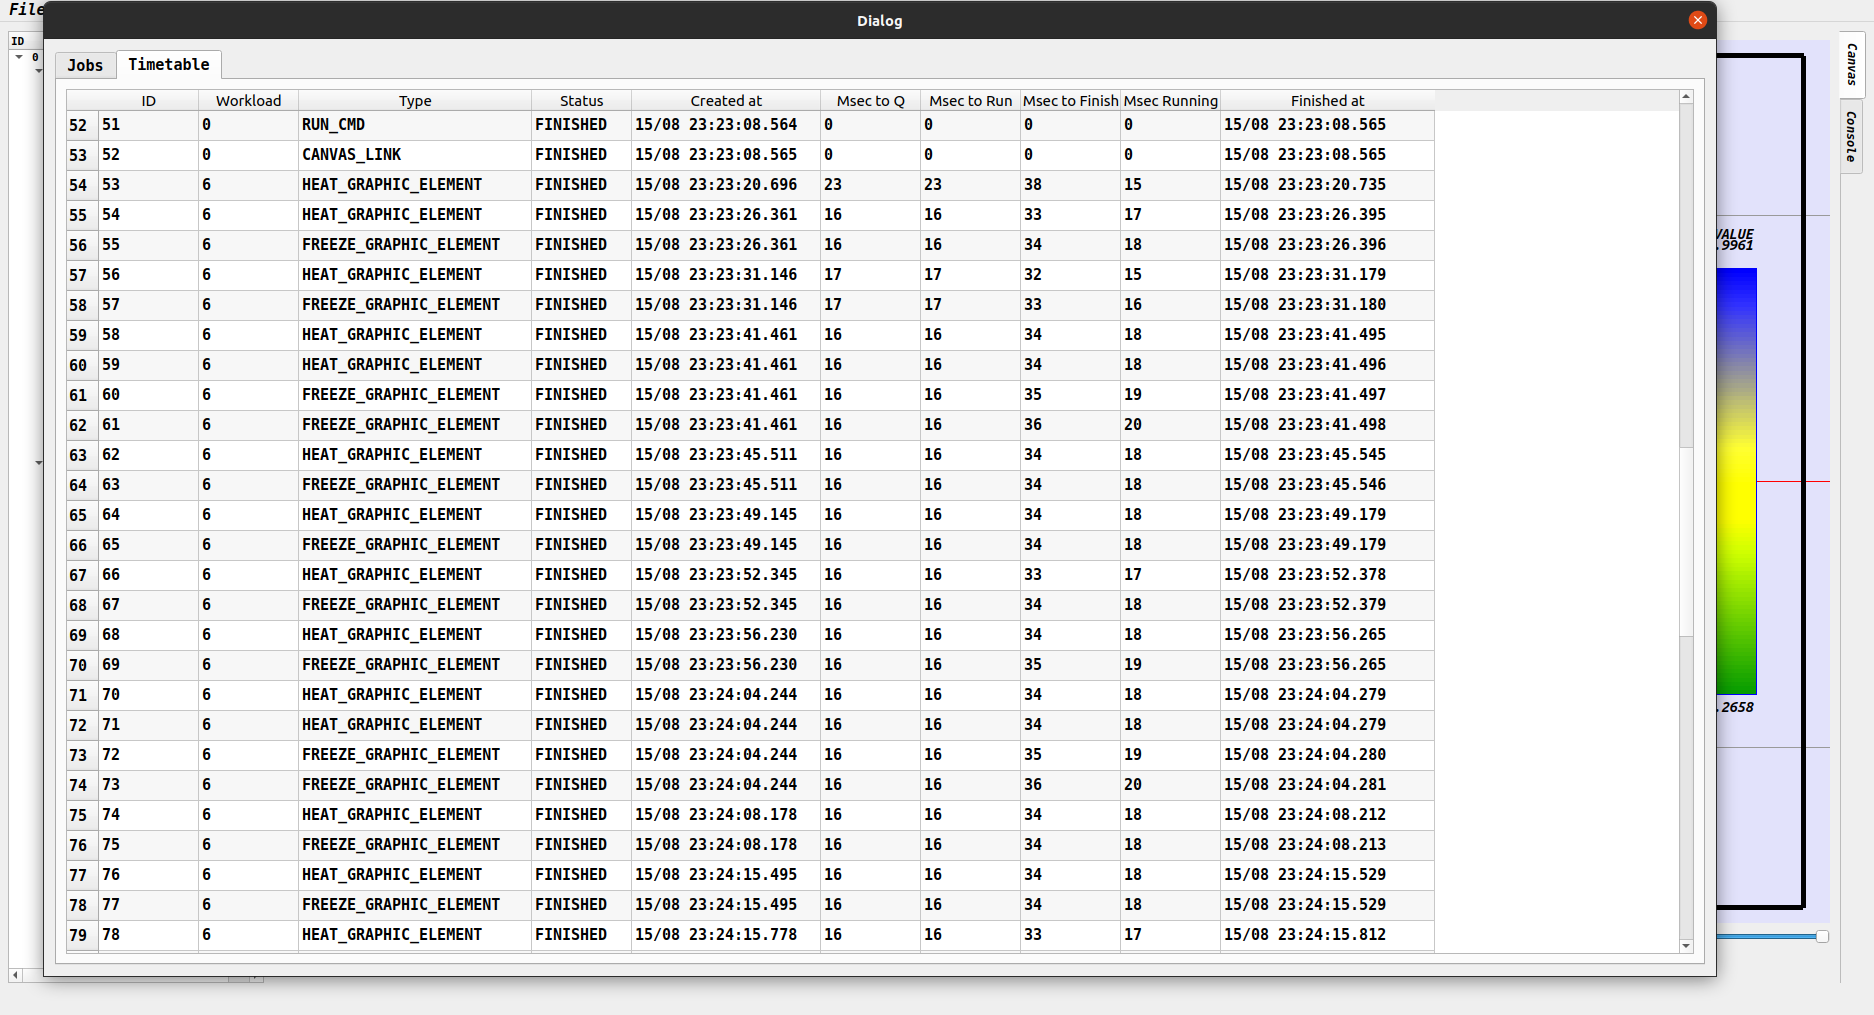
\includegraphics[width=\linewidth]{Figures/IGU_023.png}
	\caption{Janela \textit{Jobs} exibida com a aba \textit{Timetable} selecionada, a janela lista os trabalhos recebidos pela estrutura \textit{WiseThreadPool} e seus tempos de execução.}
	\label{fig:jobs}
\end{figure}

A Figura~\ref{fig:jobs} demonstra a tabela obtida lista todos os trabalhos recebidos pela thread inteligente \textit{WiseThread} e suas propriedades. Cada linha nesta janela representa um \textit{WiseJob}, as colunas descrevem propriedades de cada trabalho:

\begin{itemize}
	\item \textbf{ID}: Número de identificação.
	\item \textbf{Workload}: Número da carga de trabalho.
	\item \textbf{Status}: Estado do trabalho.
	\item \textbf{Created at}: Data de criação.
	\item \textbf{Msec to Q}: Milisegundos do momento da criação até a chegada a fila.
	\item \textbf{Msec to Run}: Milisegundos do momento da criação até a alocação do trabalho em uma thread.
	\item \textbf{Msec to Finish}: Milisegundos do momento da criação até o final de sua execução.
	\item \textbf{Msec Running}: Milisegundos no estado \textit{RUNNING}.
	\item \textbf{Finished at}: Data de finalização.
\end{itemize}

\begin{figure}[!htbp]
	\centering
	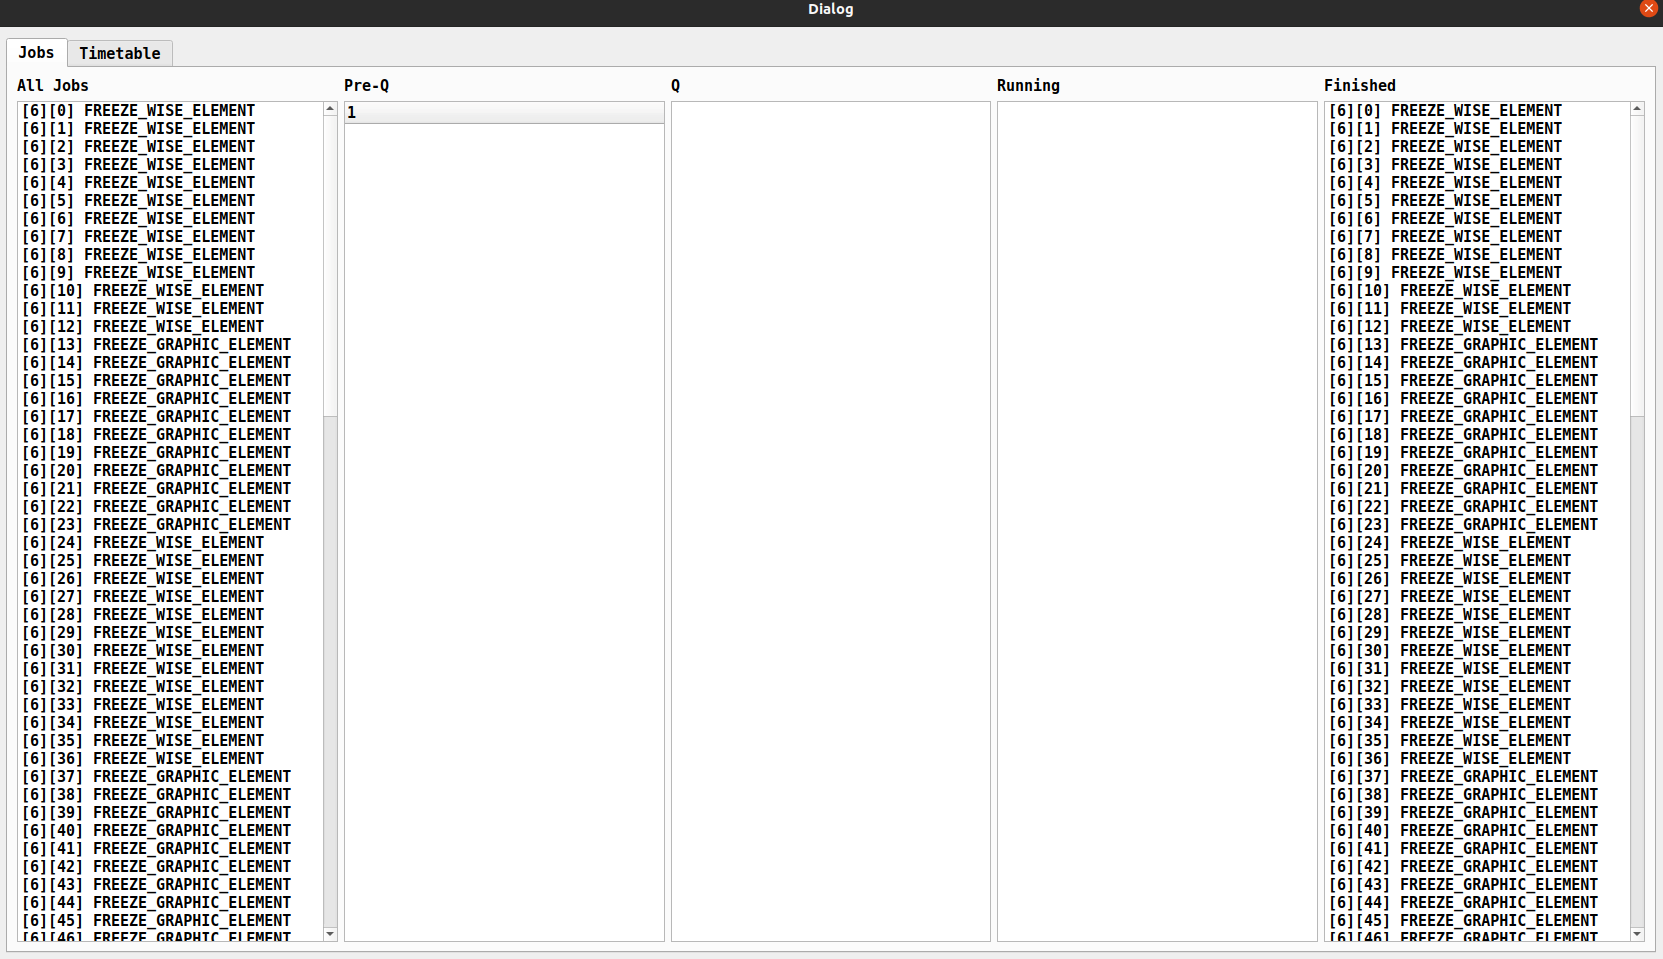
\includegraphics[width=\linewidth]{Figures/IGU_022.png}
	\caption{Janela \textit{Jobs} exibida com a aba \textit{Timetable} selecionada, a janela lista os trabalhos recebidos pela estrutura \textit{WiseThreadPool} e os separa logicamente pelas listas de espera.}
	\label{fig:jobs2}
\end{figure}

A Figura~\ref{fig:jobs2} demonstra as cinco listas exibidas ao selecionar a aba \textit{Timetable} da janela \textit{Jobs}. A primeira lista \textit{All Jobs} lista todos os trabalhos criados e as listas subsequentes listam as listas presentes no gerenciador de threads \textit{WiseThreadPool} descritas na Seção~\ref{sec:trabalhos}. Desta forma é possível verificar os trabalhos que aguardam execução, estão sendo executados e foram finalizados.
\chapter{FERRAMENTA COMPUTACIONAL}\label{sec:ferramenta_computacional}

Nesta seção apresentam-se detalhes da ferramenta computacional desenvolvida para simulação do escoamento sanguíneo em modelos de árvores arteriais. A principal finalidade desta ferramenta é possibilitar a visualização de estruturas das árvores arteriais e após a simulação hemodinâmica,  a visualização das curvas de distribuição do fluxo sanguíneo e pressão.

Esta ferramenta foi desenvolvida em C++ utilizando as bibliotecas do Qt 5.15.0 \cite{QTClasses} e OpenGL \cite{OpenGL}, que ajudam na construção da interface gráfica e na exibição de modelos gráficos, como árvores arteriais e gráficos dos resultados. A ferramenta foi disponibilizada em dois ambientes, o primeiro nomeado de \textit{Iterador Gráfico Universal} (IGU), pois em seu modelo de classes qualquer objeto que implemente a classe \textit{WiseObject} (descrito na Seção~\ref{sec:objeto_inteligente}) está apto para realizar iterações e desenhar-se através de diretivas OpenGL em um elemento de interface gráfica. O segundo ambiente disponibilizado foi nomeado de \textit{Iterador não-Gráfico Universal} (InGU), pois segue a mesma generalização, entretanto é disponibilizada pelo console, não possuindo interface gráfica. Buscou-se no desenvolvimento desta ferramenta alto grau de generalização para que seja possível analisar todos os parâmetros de um objeto facilmente e que ela possua grande versatilidade. \igunew{Além de árvores arteriais a ferramenta possibilita que outros objetos sejam gerados para visualização, qualquer objeto que implemente a classe \textit{GraphicObject} (descrito na Seção~\ref{sec:objeto_grafico}) pode ser visualizado.} A Figura~\ref{fig1:gui} ilustra a ferramenta desenvolvida.

\begin{figure}[!htbp]
	\centering
	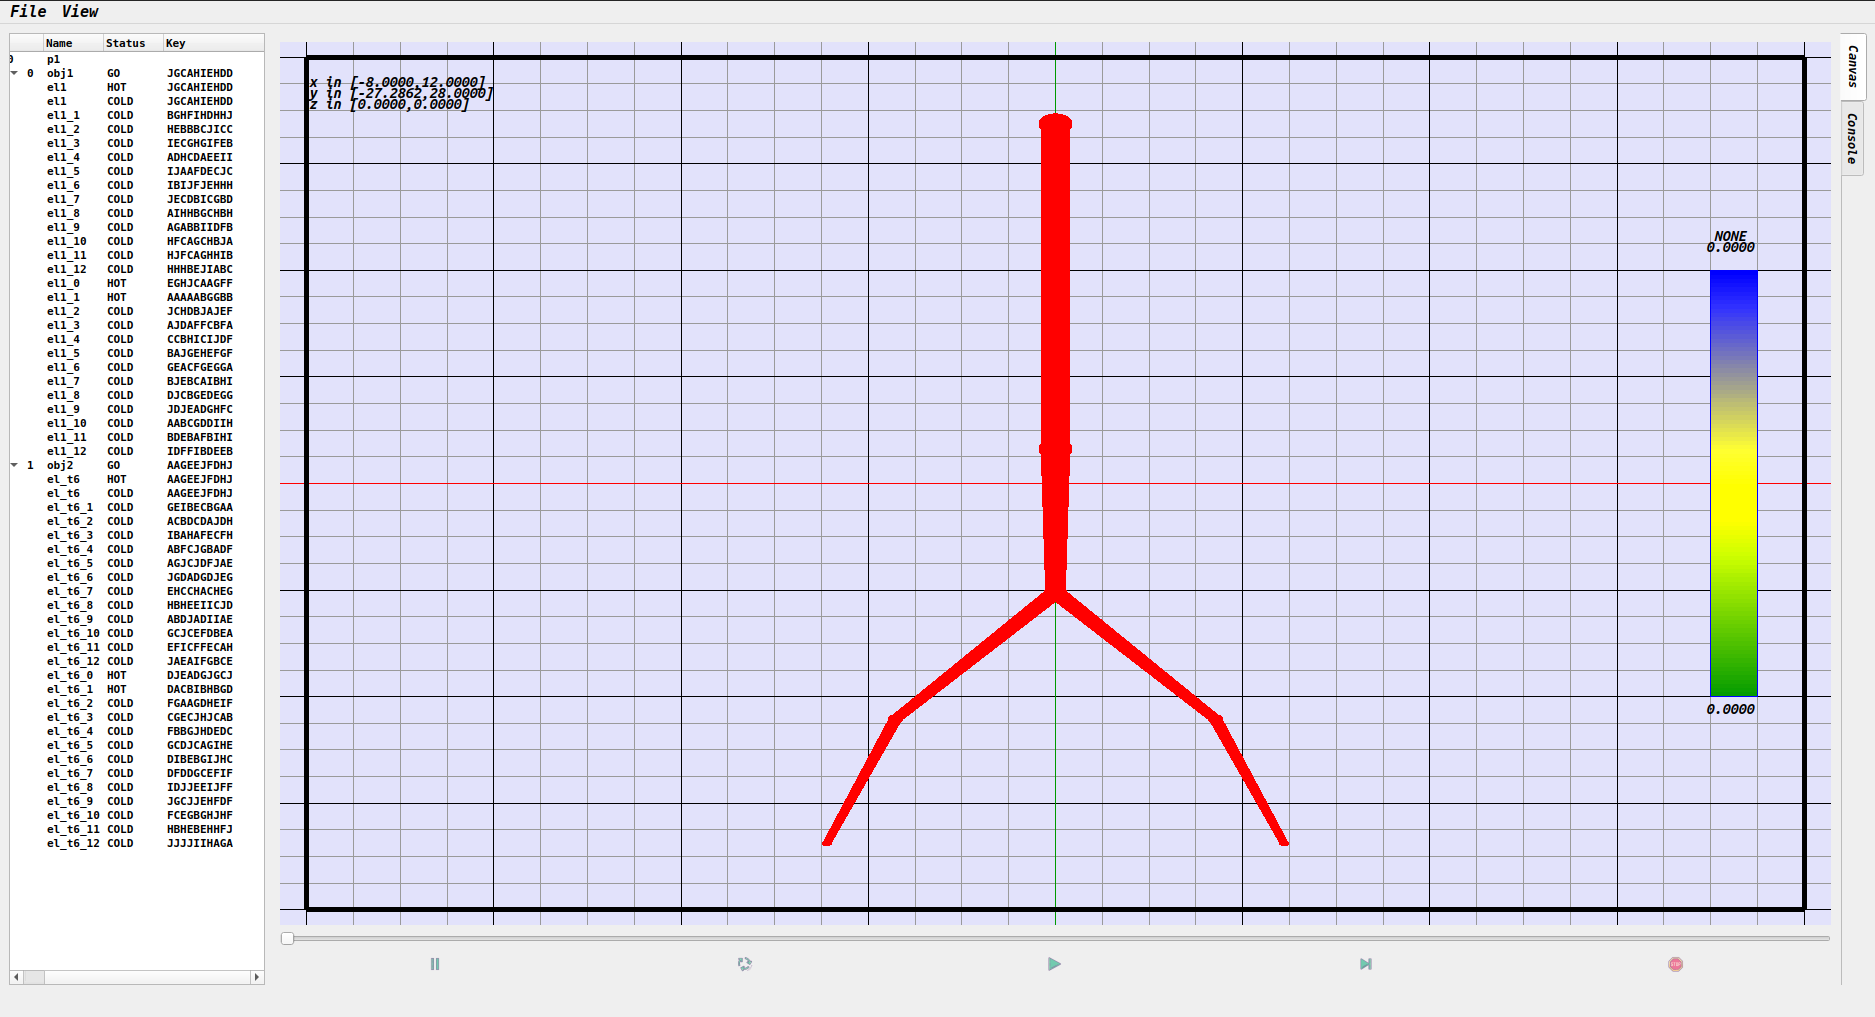
\includegraphics[scale=0.25]{Figures/IGU_002.png}
	\caption{Interface gráfica da ferramenta desenvolvida.}
	\label{fig1:gui}
\end{figure}

Através da modelagem de classes no paradigma do C++ \cite{AlanParker}, foi possível realizar diversas generalizações que ampliam a adaptabilidade dos objetos que podem ser inseridos neste modelo de classes. Na Seção~\ref{sec:estrutura} é proposto um esquema de classes virtuais, ou abstratas, que foram criadas para facilitar o manuseio dos objetos dentro do ambiente computacional e prover funções básicas. 

Uma classe virtual não possui construtor próprio, porque classes virtuais são incompletas. Estas classes possuem métodos virtuais, que por sua vez precisam ser definidos pela classe herdeira. Portanto uma classe virtual funciona como um conjunto de regras que classes herdeiras devem seguir, todas as classes que implementem esta classe virtual devem ter sua própria definição dos métodos virtuais, podendo ter funcionamentos distintos, entretanto recebendo os mesmo parâmetros.  Adicionado este conceito à estrutura de dados, classes virtuais generalizam os objetos e garantem o seu funcionamento, separando as estruturas de acordo com seu propósito em classes.

\igunew{Nesta ferramenta computacional ponteiros foram utilizados na organização destas classes virtuais, quando um ponteiro para uma classe abstrata é definido, é possível que diversas estruturas de dados sejam referencias. Ao referenciar um objeto inteligente \textit{WiseObject} através de um ponteiro é possível acessar os métodos padrões da classe abstrata que irão acessar a implementação de cada objeto. Todos os objetos inteligentes irão ter por definição um método que irá construir a estrutura, mas cada objeto irá construir suas próprias estruturas. Portanto é possível que a ferramenta computacional envie estes dados sem necessariamente reescreve-los na memória, eles são enviados por referência. Este fator foi determinante na escolha da linguagem \textit{C++}, pois um ponteiro é o endereço de memória física, o que permite uma agilidade maior na organização da ferramenta e na utilização destas estruturas pela ferramenta em suas diferentes \textit{threads}.}

%--------------------------------------------------------------------------------%
\section{MODELAGEM COMPUTACIONAL}
\label{sec:algoritmo}
%\textcolor{red}{IGOR: fiz mais uma revisão nesta seção. Cheque se tudo está coerente com o quis dizer após minhas alterações no texto.} \textcolor{green}{OK}

Nesta seção, detalham-se alguns aspectos da estrutura de dados e algoritmos que descrevem os passos para o cálculo das equações da pressão $P$ e fluxo $Q$ definidas em \eqref{21_P} \eqref{23_Q}, respectivamente.

Inicialmente, salientam-se que as Equações~\eqref{27_R} e~\eqref{28_Ye} expõem a necessidade de valores $Y_e(k+1,2j)$ e $Y_e(k+1,2j-1)$ atrelados aos vasos adjacentes na posição distal do vaso $(k,j)$. Por outro lado, o valor da pressão média do vaso $(k,j)$ calculado usando a Equação~\eqref{18_barp} depende de valores  à montante desse vaso, ou seja, do valor $\bar{p}(k-1,s)$. Tendo isto em vista, a estrutura de dados desenvolvida utiliza ponteiros para acessar as propriedades de artérias à montante e a jusante de um vaso do modelo.

Neste trabalho, adotou-se a linguagem de programação C++. Essa linguagem de programação escolhida permite que objetos sejam passados por referência. Ao passar um objeto por referência, o endereço de memória é enviado, dando total acesso aos parâmetros do objeto, este endereço é chamado de ponteiro. Ao enviar o ponteiro do vaso raiz, é possível acessar todo o modelo de árvore arterial. Cada vaso arterial do modelo contém as propriedades apresentadas na Tabela~\ref{tab:info_vaso}, além de ponteiros para os vasos adjacentes. 

\begin{table}[h]
	\begin{tabular}{c|c|c|c}
		\toprule
		\textbf{valores conhecidos} & \textbf{unidade} & \textbf{valores calculados} & \textbf{unidade} \\\midrule
		
		comprimento ($L$) & cm &  velocidade da onda ($c$) & cm/s \\
		
		densidade ($\rho$) & g/cm$^3$ &   beta ($\beta$) & -- \\
		
		módulo de Young ($E$) & g/cms$^2$  & velocidade angular ($\omega$) & rad/s \\
		
		viscosidade ($\mu_0$) & cm$^2$/s &	espessura da parede ($h$) &  $cm$ \\
		
		raio ($r$) & cm  & número de Womersley ($\alpha$) & --- \\
		
		& & admitância característica ($Y$) & $cm^4 s/g $\\
		
		&  & admitância efetiva ($Y_e$) & $cm^4 s/g $\\
		
		&  & coeficiente de reflexão ($R$) & $g /cm^4 s$ \\
		
		& & fator viscoso ($\epsilon$) & -- \\
		
		& & pressão ($P$) & -- \\
		
		&  &	pressão média ($\bar{p}$) & -- \\
		
		& &	fluxo ($Q$) & -- \\
		\hline
	\end{tabular}
	\caption{Propriedades de cada vaso arterial do modelo.}
	\label{tab:info_vaso}
\end{table}

Além das propriedades especificadas na Tabela~\ref{tab:info_vaso}, o vaso possui ainda três ponteiros para os seus vasos adjacentes. Um destes ponteiros, para o vaso adjacente ao seu nó proximal, ou seja, para o seu vaso pai $(k-1,s)$. Os demais ponteiros para os vasos adjacentes ao seu nó distal, ou seja, para seus vasos filhos à esquerda ($esq$) e à direita ($dir$) expressos por $(k+1,2j-1)$ e $(k+1,2j)$, respectivamente. Este arranjo de ponteiros é equivalente a uma árvore duplamente encadeada, onde através de um único ponteiro para um vaso é possível trafegar a árvore nos dois sentidos. Isto é útil quando é necessário acessar propriedades de outro vaso para se determinarem por exemplo, a pressão média, coeficientes de reflexão e admitâncias de um dado vaso.

Os ponteiros permitem também definir se o vaso é a raiz ou uma folha. Caso o ponteiro para o segmento superior $(k-1,s)$ seja igual ao valor da \textit{flag} nula se trata de um vaso raiz. Caso ambos vasos  $(k+1,2j-1)$ e $(k+1,2j)$ sejam iguais ao valor da \textit{flag} nula se trata de vaso folha, isto é, um vaso terminal.

Basicamente, os passos para determinar as ondas de pressão e fluxo que percorrem um modelo de árvore arterial usando o modelo de Duan e Zamir são dados por:

\begin{algorithm}[H]
	\SetAlgoLined
	\Inicio{
		Cálculo da admitância característica $(Y)$ de cada vaso;\\
		Cálculo da admitância efetiva $(Y_e)$  de cada vaso;\\
		Cálculo do coeficiente de reflexão $(R)$  de cada vaso; \\
		Armazenar valor da admitância característica $(Y_r)$ do vaso raiz, isto é, o valor de $Y(1,1)$;\\
		Cálculo da pressão média $(\bar{p})$ em cada vaso;\\
		Cálculo das ondas de pressão e fluxo $P$ e $Q$.
	}
	\caption{Cálculos hemodinâmicos simplificados com passos determinando as ondas de fluxo e pressão.}
	\label{algsimples}
\end{algorithm}

Os passos acima mencionados podem ser organizados no Algoritmo 1. Esse algoritmo tem como entrada: o modelo de árvore arterial ($\mathcal{MAA}$) com seus vasos caracterizados por suas propriedades, a frequência $f$, um fator de escala da viscosidade $\gamma_{\mu}$, o parâmetro da viscoelasticidade da parede $\phi$ e a quantidade de espaçamento para discretização de um vaso $N$.

O Algoritmo 1 proposto tem dois módulos, a saber: $\mathcal{M}_1$ e $\mathcal{M}_2$.

\begin{algorithm}[H]
	\SetAlgoLined
	\Entrada{ $\mathcal{MAA}$, $f$, $\gamma_{\mu}$, $\phi$, $\bar{p}_0$, $N$ }
	\Inicio{
		inicializa vaso $v$ a partir do vaso raiz;\\
		\Se{existe($v$)}{
			Chama $\mathcal{M}_1$ ($v$, $f$, $\gamma_{\mu}$, $\phi_0$) e armazena $Y_r$;
		}
		\Se{existe($Y(1,1)$)}{
			Chama $\mathcal{M}_2$($v$ , $\bar{p}_0$, $Y_r$, $N$);
		}
	}
	\caption{Cálculos hemodinâmicos do modelo de árvore arterial ($\mathcal{MAA}$).}
\end{algorithm}

\igunew{O módulo $\mathcal{M}_1$ realiza o cálculo percorrendo o caminho a partir dos vasos finais até o vaso raiz (estratégia do tipo \textit{bottom-up}), visando} calcular os valores de admitância efetiva ($Y_e$), admitância característica ($Y$) e coeficiente de reflexão ($R$) de cada vaso. Este módulo é definido pelo Algoritmo~\ref{AlgM1}. Necessitam-se das admitâncias efetivas dos vasos à justante do vaso $k$ ($Y_e(k+1,2j-1)$ e $Y_e(k+1,2j)$) estejam definidas. Em vista disso, verifica-se a existência dos vasos à justante do vaso atual tanto a esquerda ($esq$) quanto a direita ($dir$) e caso existam realiza-se uma chamada recursiva. Após o retorno das chamadas recursivas, calculam-se as propriedades do vaso atual. Assim, as propriedades do vasos à jusante do vaso atual serão conhecidas, ou seja, já terão sido determinadas $Y_e(k+1,2j-1)$ e $Y_e(k+1,2j)$.
\newpage

\begin{algorithm}[H]
	$\mathcal{M}_1$ ($v$, $f$, $\gamma_{\mu}$, $\phi$) \\
	\Inicio{
		\Se{existe($v \rightarrow esq$)}{
			$\mathcal{M}_1$ ($v \rightarrow esq$, $f$, $\gamma_{\mu}$, $\phi$);
		}
		\Se{existe($v \rightarrow dir$)}{
			$\mathcal{M}_1$ ($v \rightarrow dir$, $f$, $\gamma_{\mu}$, $\phi$);
		}
		Calcula as propriedades $c$, $\omega$, $\beta$; \\
		\Se{ ($\gamma_{\mu} == 0$) e ($\phi == 0$) }{
			Calcula $Y$;
		}
		\Senao{
			\Se{ ($\gamma_{\mu}~!=~0$) }{
				Calcula $\alpha$, $\epsilon$, $E_v$, $c_v$ e $Y_v$;\\
				Atualiza $E = E_v$, $c = c_v$ e $Y = Y_v$;
			}
			\Se{ ($\phi~!=~0$) }{
				Calcula $E_c$;\\
				Atualize $E = E_c$;
			}
		}
		\Se{($v$ é um vaso terminal)}{
			$Y_e = Y$ e  $R = 0$;
		}
		\Senao{
			Calcula $Y_e$ e $R$;
		}
	}
	\caption{$\mathcal{M}_1$ -- Cálculo das admitâncias e coeficiente de reflexão.}
	\label{AlgM1}
\end{algorithm}

\igunew{O módulo $\mathcal{M}_2$ realiza os cálculos percorrendo o modelo a partir do vaso raiz até os vasos terminais (abordagem do tipo \textit{top-bottom}), visando} calcular o valor da pressão média, pressão e fluxo em cada vaso. Este módulo é expresso no Algoritmo~\ref{AlgoritmoM2}. Como expresso na Equação~\eqref{18_barp}, o valor da pressão média requer o valor da pressão média do vaso à montante $(k-1,s)$. Com isso, inicialmente, se o vaso atual é a artéria de alimentação (raiz), neste caso $\bar{p} = \bar{p}_0$. Caso contrário, calcula-se $\bar{p}$ com a Equação~\eqref{18_barp}. Em seguida, o valor das ondas de pressão e fluxo são obtidas ao longo de cada vaso 1D, que são discretizados. Por fim, a recursão é enviada aos segmentos inferiores, desta forma se garante a existência de um valor $\bar{p}(k-1,s)$.

\begin{algorithm}[H]
	$\mathcal{M}_2$ ($v$, $\bar{p}_0$, $Y_r$, $N$) \\
	\Inicio{
		\Se{ ($v$ é o vaso raiz)}{
			$\bar{p} = \bar{p_0}$;
		}
		\Senao{
			Calcula $\bar{p}$;
		}
		Calcula $P(X_i)$ e $Q(X_i)$, onde $X_i \in [0,1]$; \\
		\Se{existe( $v \rightarrow esq$ )}{
			$\mathcal{M}_2$ ($v \rightarrow esq$, $\bar{p}_0$, $Y_r$, $N$);
		}
		\Se{existe($v \rightarrow dir$)}{
			$\mathcal{M}_2$ ($v \rightarrow dir$, $\bar{p}_0$, $Y_r$, $N$);
		}
	}
	\caption{$\mathcal{M}_2$ -- Cálculo da pressão e fluxo ao longo de cada vaso.}
	\label{AlgoritmoM2}
\end{algorithm}

No Algoritmo \ref{AlgoritmoM2} tem-se que $N$ denota a quantidade de espaçamento $dX$ no intervalo [0,1] para discretização de um vaso. Assim, $dX = 1/N$ e $X_i = i dX (i = 0, 1, \cdot\cdot\cdot, N)$.

%--------------------------------------------------------------------------------%
\section{ESTRUTURA DE DADOS}\label{sec:estrutura}

Nesta seção apresentam-se detalhes da estrutura de dados adotada no funcionamento da ferramenta computacional. Como mencionado na Seção~\ref{sec:algoritmo}~\igunew{, foi empregado uma estrutura para armazenar todas as referências às informações} do modelo geométrico da árvore arterial.

\igunew{Iterar o modelo matemático na ferramenta computacional equivale à aplicar um objeto inteligente a sua fábrica de iteração \textit{WiseIterationFactory}(descrito na Seção~\ref{sec:fabrica}). A fábrica de iteração \textit{DuanAndZamirIterationFactory} acoplada à uma árvore arterial \textit{WiseArterialTree} é equivalente a execução do~\ref{algsimples} em todo o modelo geométrico, definindo a onde de pressão $P$ e fluxo $Q$ em todos os segmentos.}

\igunew{ A ferramenta computacional foi desenvolvida para ser capaz de armazenar, carregar e iterar o modelo matemático e gerar novas estruturas para visualização, a estrutura de dados proposta para a ferramenta precisa realizar estar operações e armazenar corretamente os dados gerados.}

As seções \igunew{contidas nesta Seção de estrututra de dados} descrevem a estrutura de dados genérica, tendo como principal objeto de estudo, o fluxo pulsátil enquanto atravessa uma estrutura de árvore arterial e a visualização de seus resultados. Em versões anteriores, a ferramenta computacional definia seus modelo matemáticos, geométricos e de visualização em apenas uma estrutura abstrata, o que acarretou em classes grandes com difícil manutenção e pouca versatilidade. Isto porque o mesmo objeto ficava responsável por diversas funções, era capaz de se instanciar, iterar e desenhar na tela através de diretivas OpenGL. Portanto, nesta versão da ferramenta computacional as classes foram desenvolvidas para ter propósito único, cujo objetivo é garantir que as classe tenham uma função apenas, garantindo uma classe enxuta e de fácil interpretação.

Com a experiência adquirida previamente três principais fluxos foram identificadas:  A iteração dos objetos, uma vez carregados estes objetos são atualizados por algoritmos, gerando novas versões; O armazenamento dos objetos, os elementos criados no método de iteração podem ser armazenados em uma cache e então recuperados;  \igunew{E a exibição dos objetos, os elementos carregados podem ter seus parâmetros visualizados em um elemento de interface gráfica \textit{OpenGL}. O ciclo iterativo irá gerar ao final uma animação, cada iteração irá gera um quadro desta animação. O objeto inteligente \textit{WiseObject} irá armazenar todos estes quadros, cada quadro representa um elemento inteligente \textit{WiseElement}.} Cada quadro antes de ser exibido precisa ser processado em diretivas OpenGL, o responsável sobre esse processo é o elemento gráfico \textit{GraphicObject}. Igualmente quando se tratam de animações e reproduções de vídeo, somente quadros necessários estarão em memória. 

Finalmente, estas estruturas são utilizadas pela ferramenta computacional possibilitando que modelos geométricos sejam carregados, iterados e então exibidos, sem que haja perda dos quadros ou de algum dado. Os elementos principais da estrutura de dados serão descritos nas seções que se seguem.

%--------------------------------------------------------------------------------%
\subsection{ELEMENTO INTELIGENTE}\label{sec:elemento_inteligente}

Elementos inteligentes são objetos que implementam a classe \textit{WiseElement}, o principal objetivo de um elemento inteligente é manter os dados mais recentes de um modelo geométrico e os dados necessários para o método de iteração. No caso do estudo do fluxo pulsátil consideramos que uma iteração seja a execução completa do algoritmo apresentado na Seção~ \ref{sec:algoritmo} em toda a árvore. Portanto cada elemento inteligente possuirá todas as informações do modelo geométrico de uma árvore arterial, seus segmentos e suas propriedades.

Através das malhas estruturadas e desestruturadas presentes na biblioteca \textit{VTK}(\textit{Visua}-\textit{lization ToolKit})~\cite{VTKUSER} é possível descrever diversas estruturas de dados através de elementos padronizados, como pontos, linhas e células. Utilizando os elementos básicas contidas nestas malhas, variáveis e ferramentas da linguagem a estrutura básica da arquitetura foi criada, presente na Figura~\ref{fig2:wiselement}.

\begin{figure}[!htbp]
	\centering
	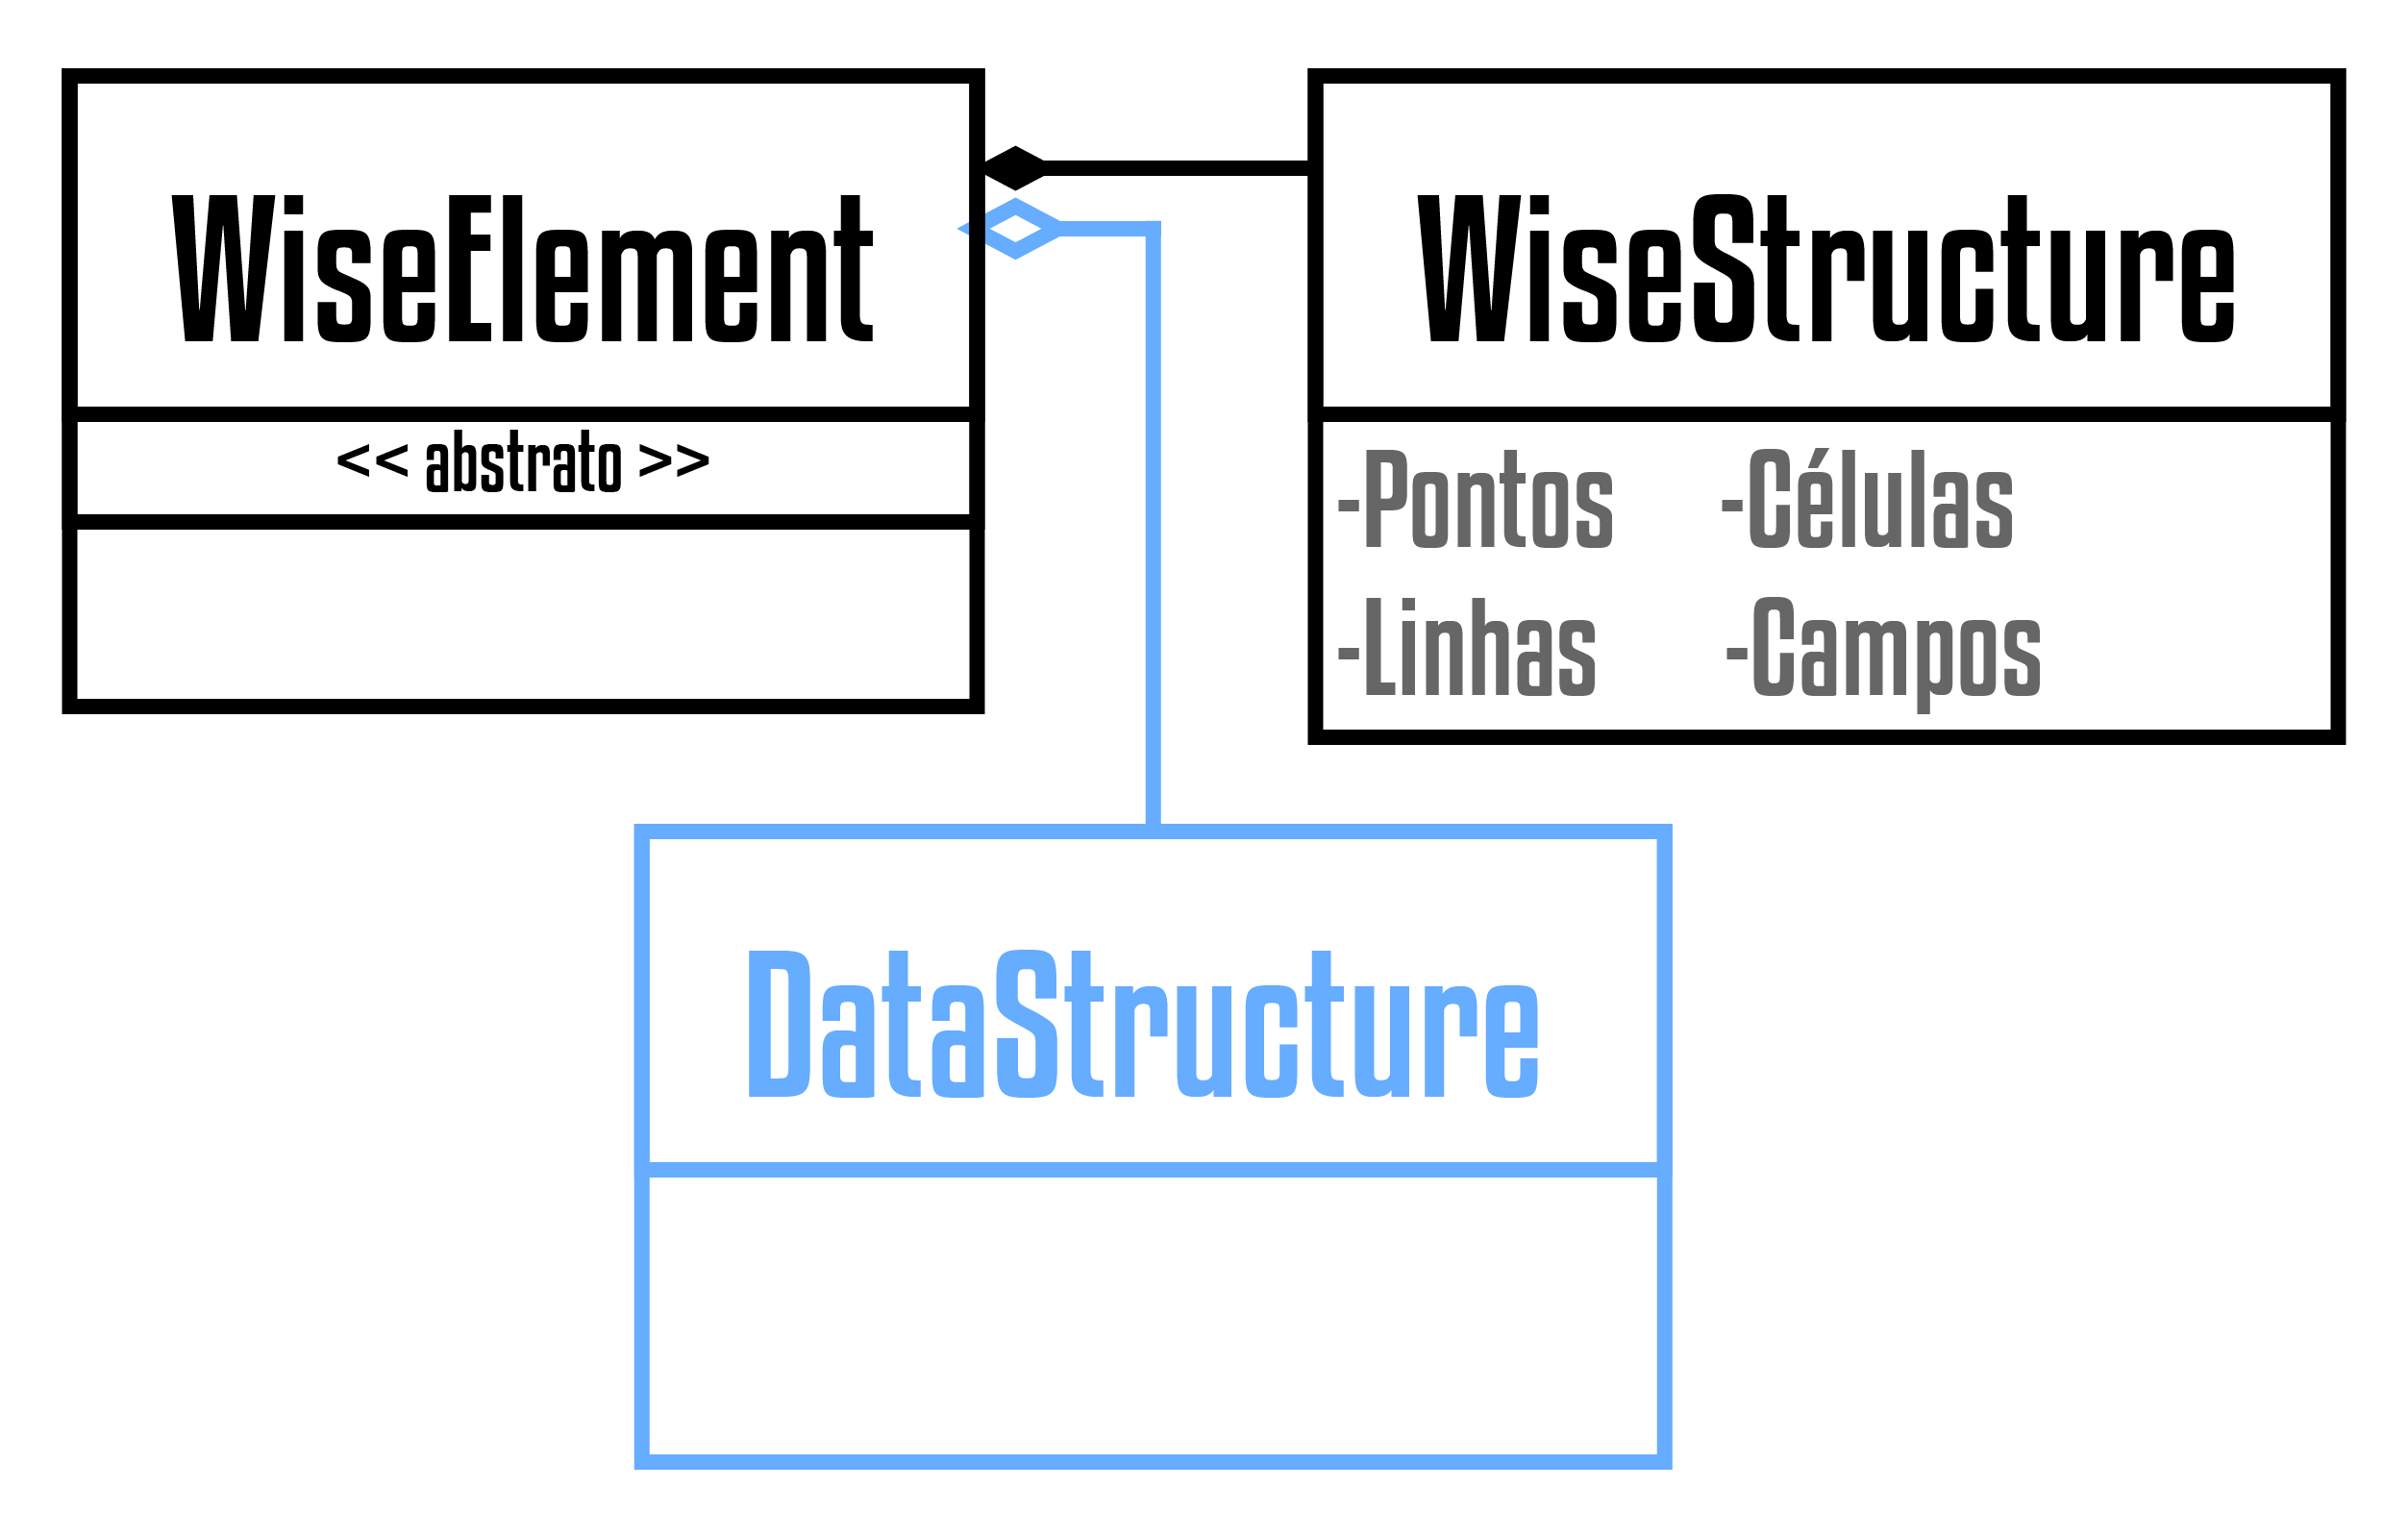
\includegraphics[scale=2]{Figures/WiseElement@16x.png}
	\caption{Representação de classes de um elemento inteligente. \textit{WiseElement} a classe abstrata base e seus componentes: \textit{WiseStructure} representa a estrutura contida em um arquivo VTK e DataStructure representa a estrutura de ponteiros e variáveis utilizadas na iteração. Tingido de azul as estruturas que nem sempre estão presentes.}
	\label{fig2:wiselement}
\end{figure}

A Figura~\ref{fig2:wiselement} mostra que um elemento inteligente é composto por duas outras estruturas: A primeira \textit{WiseStructure}, utiliza pontos, linhas, células e campos para determinar estruturas geométricas; A segunda \textit{DataSructure}, representa os dados abstratos específicos de cada elemento. Estas estruturas são equivalentes entre si, isto é feito para que a primeira estrutura siga um formato padrão de pontos, linhas, células e campos seja mantida. Enquanto dados abstratos equivalentes podem ser utilizados. Os dados mantidos na estrutura padrão \textit{WiseStructure} são utilizados principalmente na leitura e escrita de objetos, portanto são mantidos como vetores que possuem cadeias de caracteres, os dados presentes nesta estrutura podem ser editados pelo usuário. Enquanto os dados abstratos contém a mesma informação contida em variáveis da linguagem, como números inteiros, vetores, ponteiros e outros.

Cada parâmetro de um elemento inteligente representa uma grandeza associada à um componente do modelo geométrico (pontos,  linhas e células) ou ainda sobre todo o modelo (campos). \igunew{Os parâmetros armazenam valores definidos por um nome e uma referência ao modelo geométrico, os raios $r$ de um árvore arterial são dados relacionados à um segmento que é representado por uma linha, como só existe um raio por segmento, somente um valor será armazenado. Os valores da onda de uma onda de pressão $P$ através de um segmento com $X \in [0,1]$ estão relacionados as mesmas linhas, mas são representados por uma sequência de valores. A estrutura de parâmetros permite que sejam armazenados um ou múltiplos valores no mesmo local e os acesse da mesma forma. Ao acessar o valor do raio $r$ de um segmento é recebido um vetor com apenas uma posição e ao acessar a pressão $P$ são esperados $N$ elementos.}

\begin{figure}[!htbp]
	\centering
	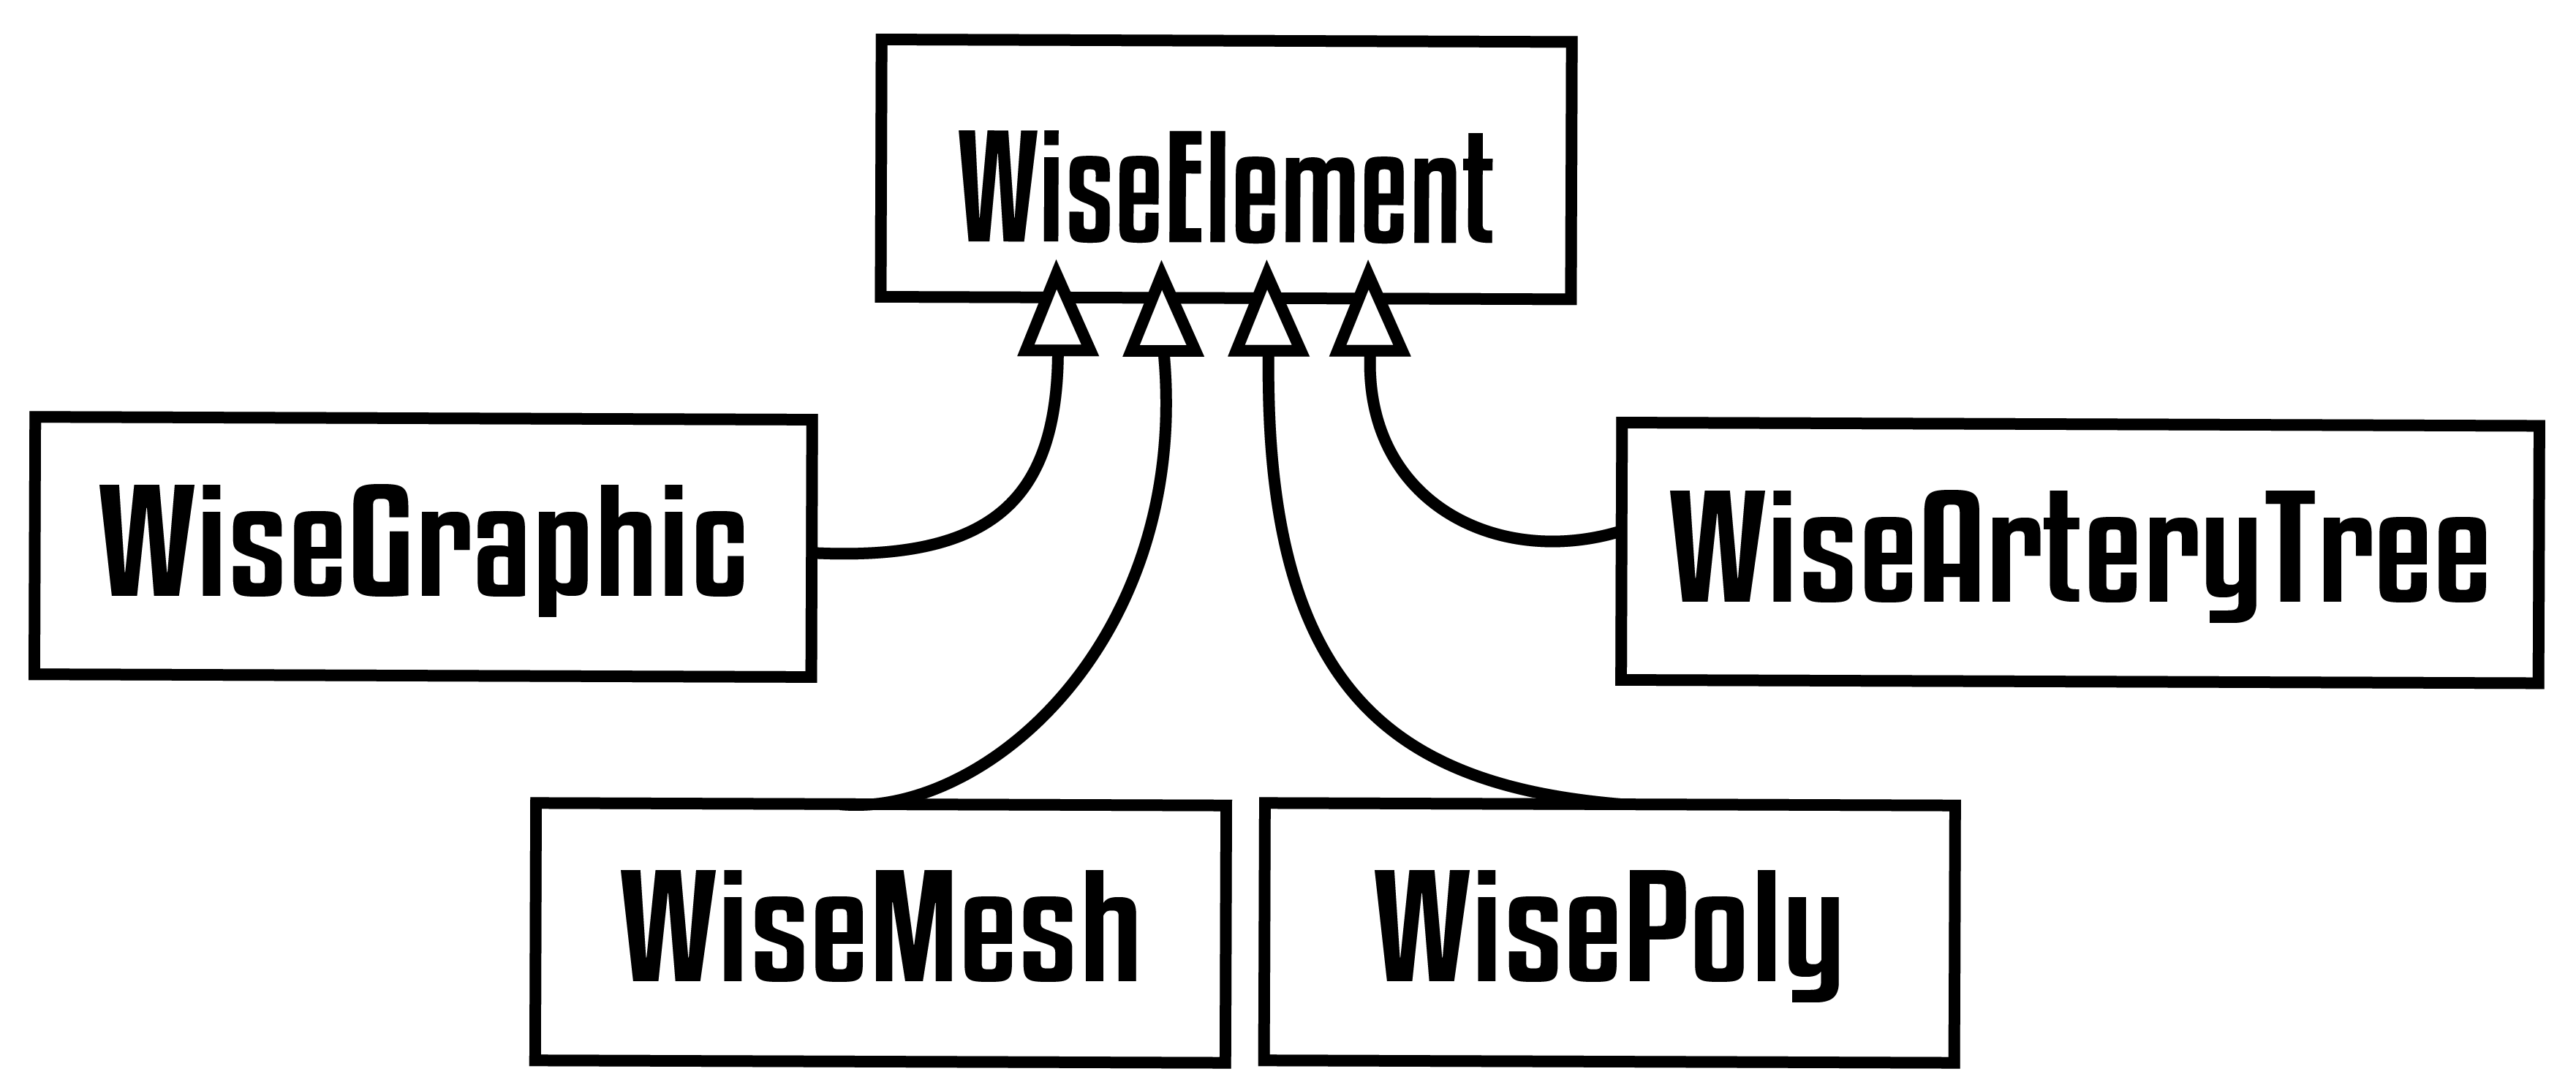
\includegraphics[width=\textwidth]{Figures/WiseElements@16x.png}
	\caption{Tipos de elementos inteligentes. \textit{WiseGraphic}, um gráfico bidimensional. \textit{WiseMesh}, uma malha tridimensional. \textit{WisePoly}, um cubo. \textit{WiseArteryTree}, uma árvore arterial}
	\label{fig2:wiselements}
\end{figure}

Como demonstrado na Figura~\ref{fig2:wiselements} um elemento inteligente é aquele que implementa a classe abstrata \textit{WiseElement}, os dados abstratos \textit{DataStructure} de cada classe podem ser salvos na estrutura padrão \textit{WiseStructure} e utilizados quando necessário. 

O modelo geométrico de uma árvore arterial foi traduzido para o elemento inteligente \textit{WiseArteryTree}, a estrutura inteligente deste elemento conta com pontos e linhas que definem os parâmetros do modelo geométrico na estrutura \textit{WiseStructure}, a estrutura abstrata \textit{DataStructure} conta com ponteiros para cada segmento e grandezas físicas armazenadas em pontos flutuantes de precisão dupla.

\igunew{Foram criadas ainda outros elementos inteligentes, como o gráfico inteligente \textit{WiseGraphic} que representa um gráfico, a malha plana inteligente \textit{WiseMesh} representa um plano e malha em cubo inteligente \textit{WisePoly} representa um cubo.}

O elemento inteligente \textit{WiseGraphic} foi criado para armazenar dados ao longo de uma dimensão, como a pressão ao longo da árvore arterial. Os elementos \textit{WiseMesh} e \textit{WisePoly} foram criados para armazenar dados ao longo de duas dimensões e ao longo de três dimensões, estes dois elementos foram utilizados como exemplo de objetos que podem ser generalizados na ferramenta e visualizados, mudando pouco as estruturas já existentes. O elemento \textit{WiseGraphic} é equivalente à um vetor de valores $(x,v)$, o elemento \textit{WiseMesh} é equivalente à uma matriz de valores $(x,y,v)$ e o elemento \textit{WisePoly} é equivalente uma matriz tridimensional de valores $(x,y,z,v)$, onde $v$ é o valor associado e $(x)$,$(x,y)$ ou $(x,y,z)$ a posição, respectivamente. Através deste modelo, é possível armazenar em um \textit{WiseMesh} o valor $v$ da pressão ao longo de uma árvore arterial na direção $x$ variando a frequência no eixo $y$.

Os elementos inteligentes servem como estruturas de armazenamento padrão que compõem um outro objeto. O ciclo de manipulação desses elementos se divide em três partes: A criação, aonde os objetos podem ser criados à partir de exemplos pré-definidos ou através de um arquivo de entrada \textit{VTK} ou \textit{XML (eXtensible Markup Language)}; A iteração, processo em que o elemento inteligente com todas as estruturas definidas e consistentes é utilizado por um algoritmo; \igunew{A exibição, este último ciclo utiliza os dados armazenados nesta estrutura e gera um objeto para visualização.}

Todo elemento inteligente completo possui uma redundância de dados, podendo ser representado por qualquer uma das duas estruturas que o compõe. A estrutura inteligente, \textit{WiseStructure}, utiliza componentes simples para descrever as estruturas e seus parâmetros. Essa estrutura é a que mais se assemelha à encontrada na arquitetura \textit{VTK}. Por utilizar uma quantidade limitada de diretivas o arquivo proveniente dessa estrutura pode ser rapidamente lido, interpretado e até mesmo exportado.

\begin{figure}[!htbp]
	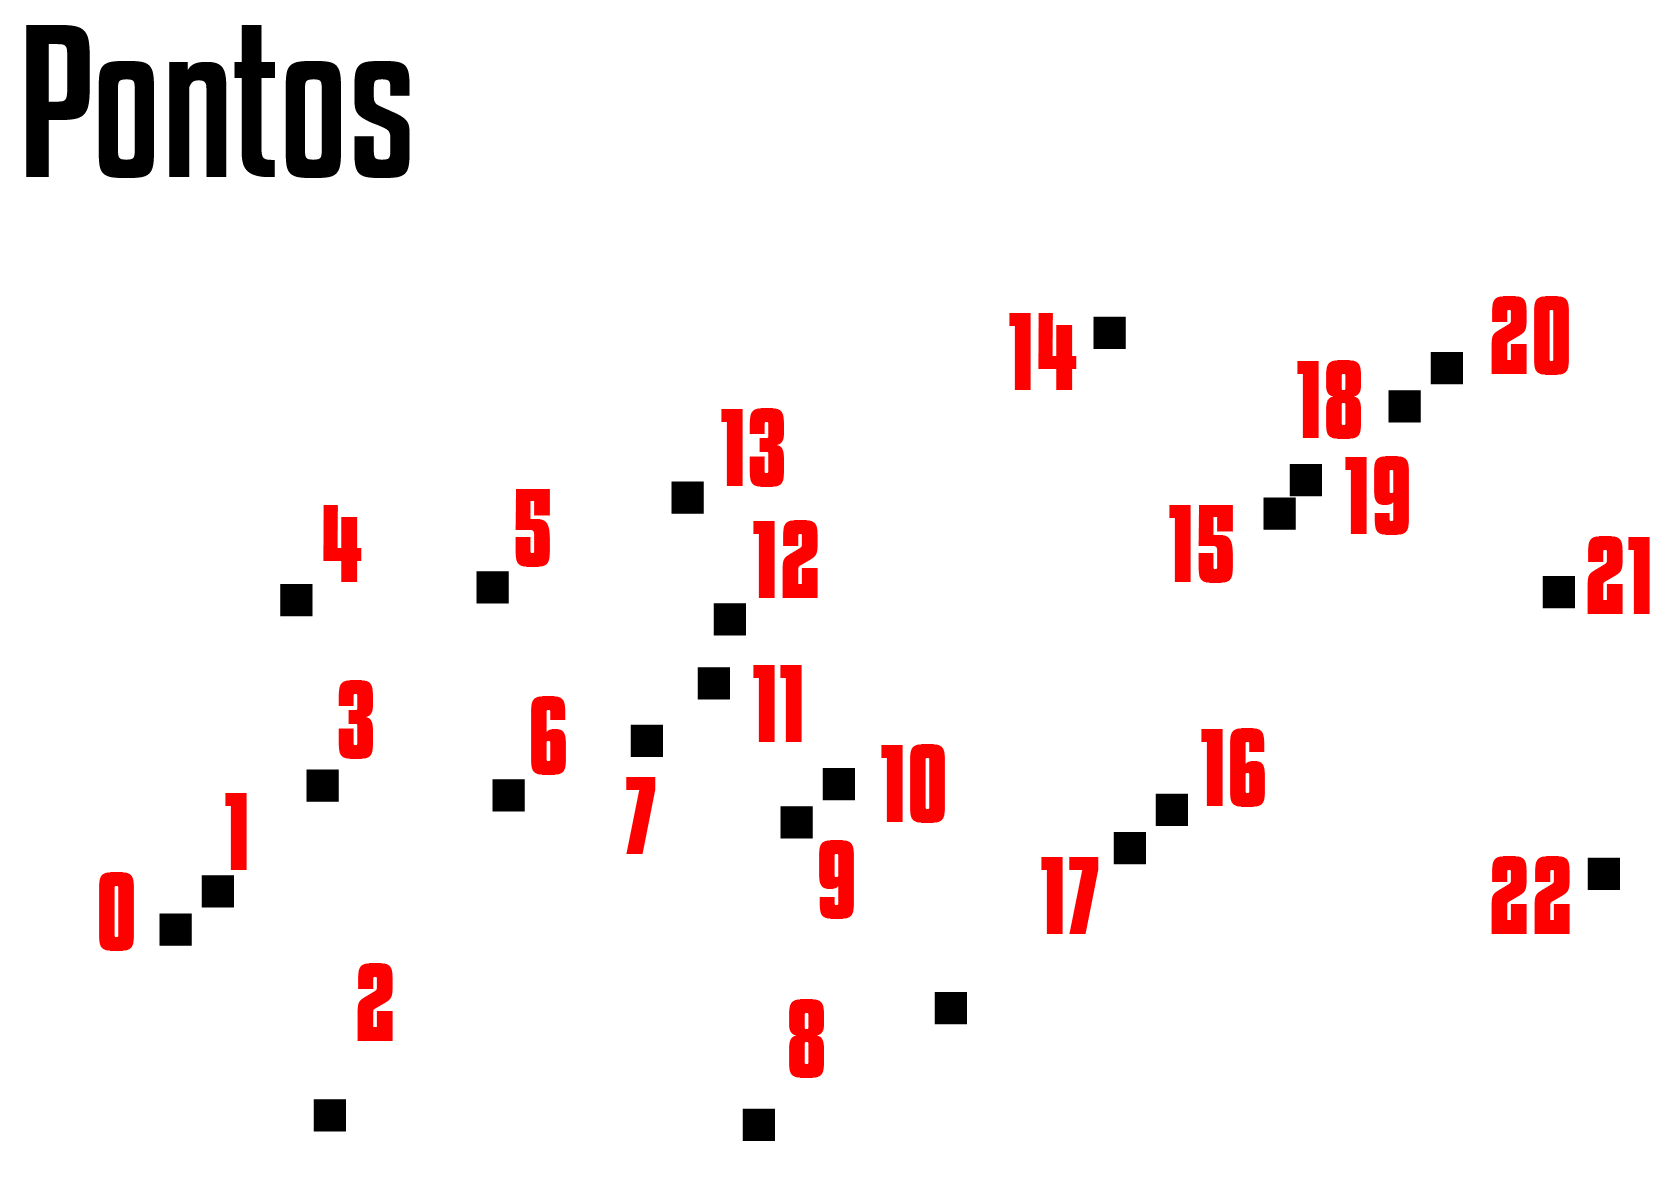
\includegraphics[width=0.5\textwidth]{Figures/WiseElementPoints@16x.png}
	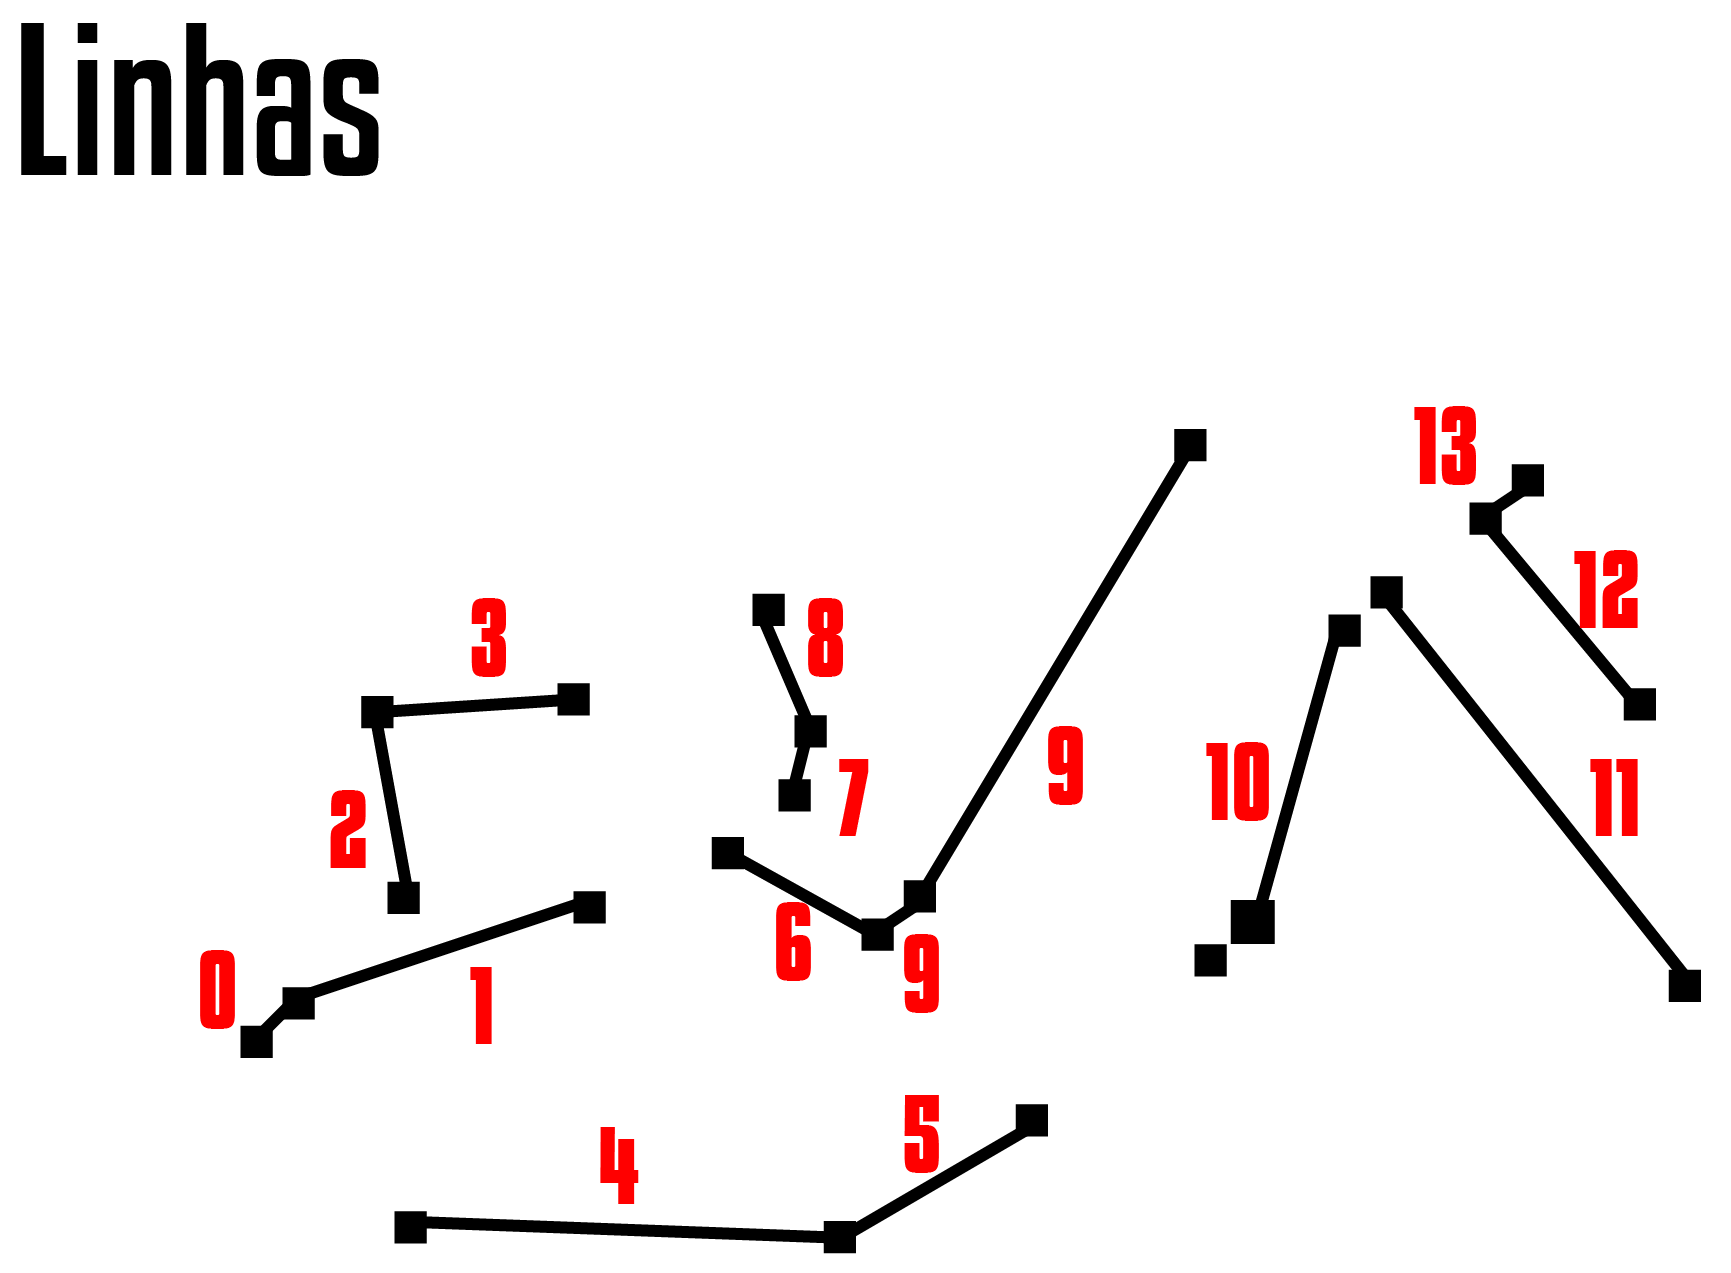
\includegraphics[width=0.5\textwidth]{Figures/WiseElementLines@16x.png}
	
	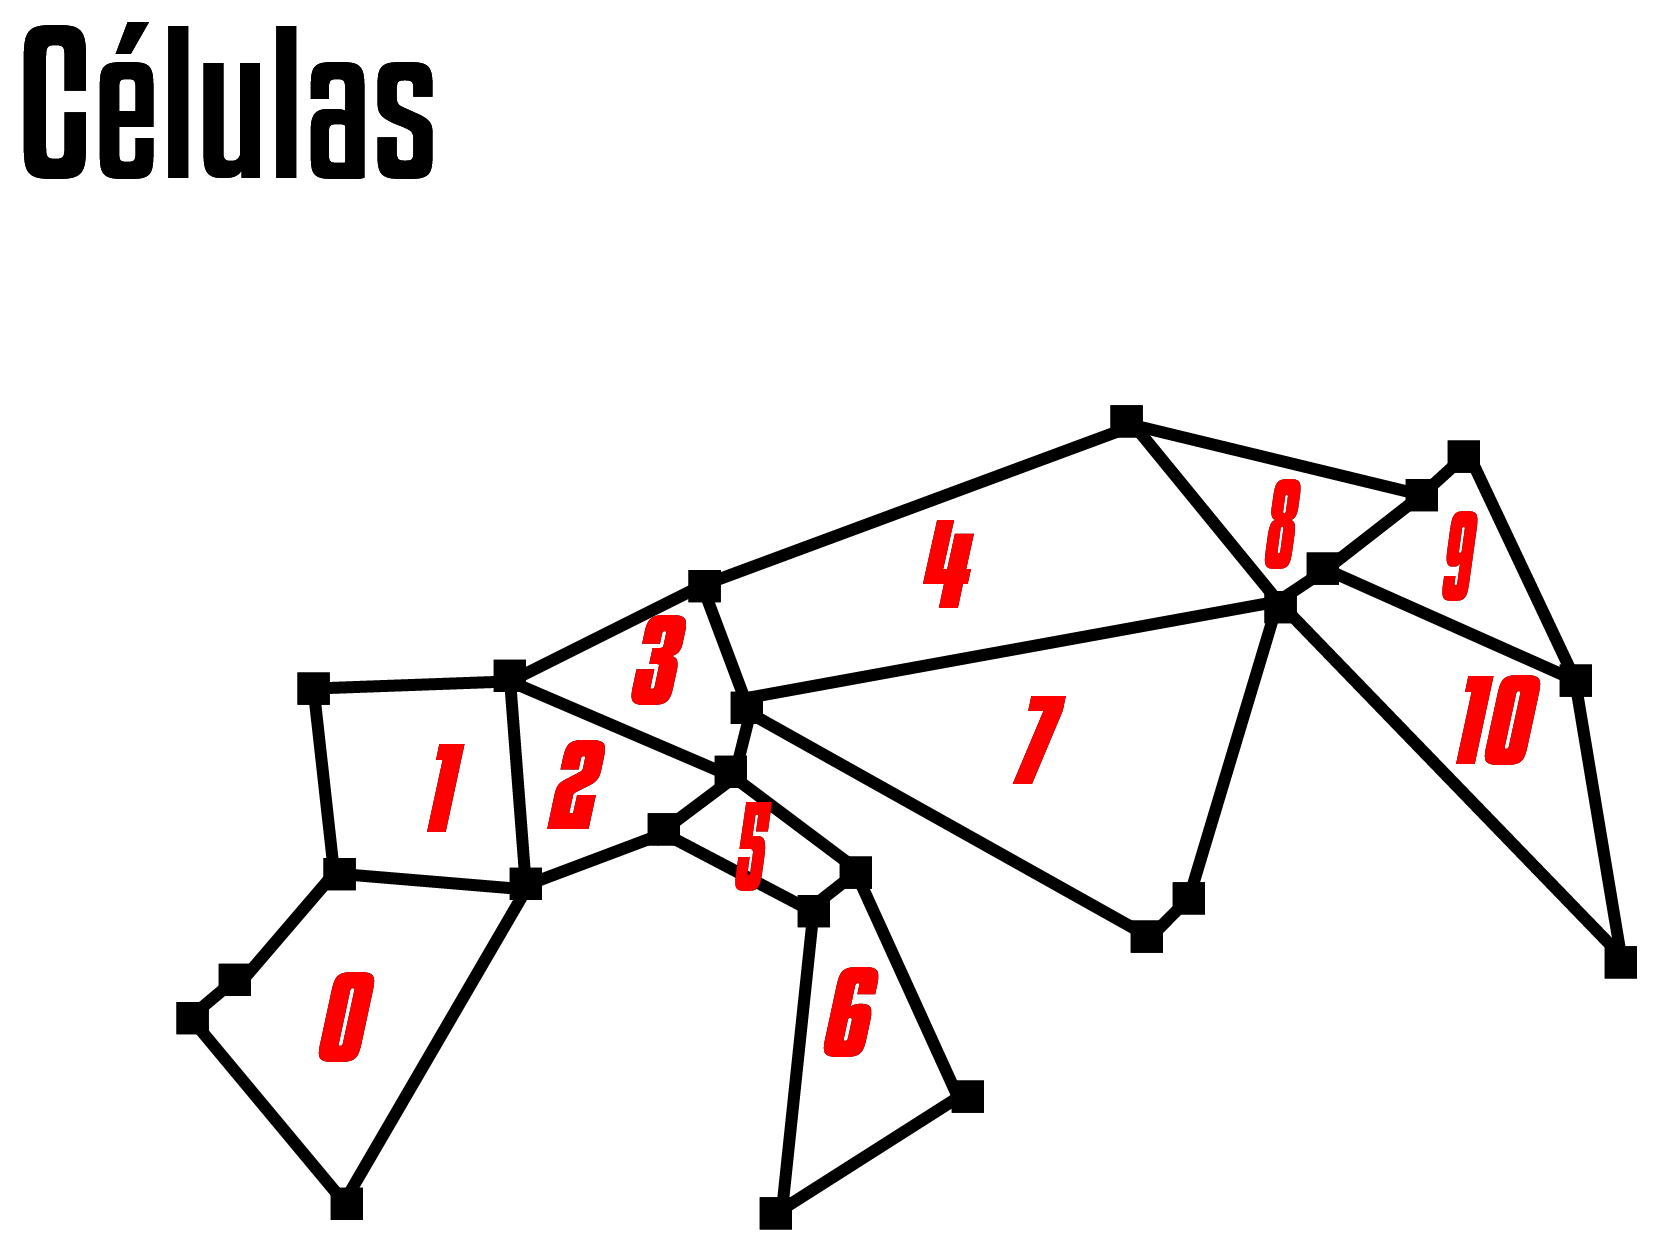
\includegraphics[width=0.5\textwidth]{Figures/WiseElementCells@16x.png}
	\caption{Pontos utilizados na especificação do modelo geométrico. Linhas utilizadas na especificação do modelo geométrico, através dos pontos previamente definidos. Células utilizadas na especificação do modelo geométrico, através dos pontos previamente definidos.}
	\label{fig2:wiselementstructs}
\end{figure}

Os componentes de uma estrutura inteligente são pontos, células, linhas e campos. Pontos demarcam uma posição no espaço, células e linhas representam conjuntos de pontos e os campos são dados gerais da estrutura. Um modelo de pontos e linhas é capaz de representar o mesmo modelo geométrico de uma árvore arterial, basta considerar cada ponto uma bifurcação de vasos e cada segmento de vaso uma linha. Através destes componentes é possível armazenar e acessar dados sobre cada segmento. Para dados gerais do modelo, como a frequência $f$, são utilizados os campos da estrutura inteligente.

A classe \textit{WiseElement} foi desenvolvida para construir a estrutura abstrata (\textit{DataStructure}) à partir das informações contidas na estrutura inteligente (\textit{WiseStructure}), desta forma é importante que a estrutura inteligente possa ser armazenada e recuperada rapidamente. O elemento inteligente é o elemento básico do método de iteração, sendo duplicado antes de ser iterado, gerando novas estruturas inteligente e abstrata idênticas. Imediatamente, a nova estrutura abstrata \textit{DataStructure} é descartada e os dados contidos na nova estrutura inteligente \textit{WiseStructure} são armazenados. Portanto, a estrutura abstrata não estará sempre presente. Seguindo este ciclo de vida, todos os elementos inteligentes obedecem à máquina de estados contida na Figura~\ref{fig3:wiselementstatus}.

\begin{figure}[!htbp]
	\centering
	\includegraphics[scale=1.5]{Figures/WiseElementStatus@16x.png}
	\caption{Máquina de estados que controla o funcionamento de um elemento inteligente.}
	\label{fig3:wiselementstatus}
\end{figure}

A máquina de estados dos elementos inteligentes gerencia o ciclo de vida de todos os elementos inteligentes, elementos inicialmente recebem o estado \textit{Raw}, ou cru, que representa um elemento ainda sem estruturas carregadas ou sem consistência garantida. Uma vez que a estrutura inteligente é inserida e verificada o elemento muda para o status \textit{Warming} ou \textit{Cooling}, respectivamente esquentando ou esfriando, suas estruturas estão representadas na Figura~\ref{fig4:wiselementwarming}.

\begin{figure}[!htbp]
	\centering
	\includegraphics[scale=1.85]{Figures/WiseElementWarming@16x.png}
	\caption{Elemento inteligente enquanto no estado \textit{Warming}, \textit{Raw} e \textit{Cooling}.}
	\label{fig4:wiselementwarming}
\end{figure}

A figura~\ref{fig4:wiselementwarming} mostra as estruturas presentes em elementos no estado \textit{Warming} que é a mesma dos estados \textit{Raw} e \textit{Cooling}. Cada estado possui uma finalidade diferente e representa em que estado estão as informações do elemento inteligente. Elementos no estado \textit{Warming} estão aguardando a construção de sua estrutura abstrata, enquanto elementos  no estado \textit{Cooling} aguardam que seus dados sejam salvos em cache. Finalmente, elementos no estado \textit{Raw} indicam que não é esperada a consistência dos dados.

Inicialmente os elementos inteligentes são criados no estado \textit{Raw}, enquanto os dados do elemento são carregados ele permanecerá neste estado. Ao final do carregamento o objeto trocará de estado para \textit{Warming} ou \textit{Cooling}, que indicam o próximo passo do elemento. Estar no estado \textit{Warming} indica que o objetivo é esquentar o objeto, atingindo o estado \textit{Hot}. Enquanto o estado \textit{Cooling} indica que a estrutura inteligente aguarda resfriamento, atingindo o estado \textit{Cold}. Quando os dados abstratos são criados corretamente para o elemento inteligente seu estado é definido como \textit{Hot}, neste estado todas as informações do objeto estão em memória, sendo este o estado mais pesado do elemento inteligente. Em contraponto, o estado \textit{Cold} indica que a estrutura inteligente foi corretamente armazenada em disco, elementos inteligentes neste estado estão em seu estado mais leve, pois possuem em memória apenas o caminho para a estrutura inteligente armazenada.

Como demonstrado na Figura~\ref{fig3:wiselementstatus}, o estado frio (\textit{Cold}) está associado com o uso de uma cache para estruturas inteligentes. A estrutura do arquivo é equivalente à uma malha estruturada VTK, mas são efetivamente salvos em um arquivo \textit{XML}. Caso sejam novamente carregados por uma mudança de estado ou deletados o arquivo armazenado é deletado. 

\begin{figure}[!htbp]
	\centering
	\includegraphics[scale=1.85]{Figures/WiseElementCold@16x.png}
	\caption{Elemento inteligente enquanto no estado \textit{Cold}.}
	\label{fig5:wiselementcold}
\end{figure}

O estado \textit{Crashed} serve para identificar objetos que não tem mais o funcionamento esperado. Durante a troca de estados do elemento é verificado se as estruturas esperadas estão presentes, caso não estejam o objeto é direcionado à este estado.

Finalmente, o estado \textit{Hot} representa os elementos que possuem todas as estruturas presentes. Isto significa que a estrutura inteligente \textit{WiseStructure} e a estrutura abstrata equivalente \textit{DataStructure} estão presentes e são consistentes.

\begin{figure}[!htbp]
	\centering
	\includegraphics[scale=1.85]{Figures/WiseElementHot@16x.png}
	\caption{Elemento inteligente enquanto no estado \textit{Hot}.}
	\label{fig6:wiseelementhot}
\end{figure}

Para que um elemento possa ser iterado ele precisa estar no estado \textit{Hot}, porque durante a iteração de um elemento inteligente seus dados abstratos são utilizados. A cada passo da iteração a estrutura \textit{DataStructure} é atualizada, exigindo uma atualização da estrutura \textit{WiseStructure}.

Seguindo o conceito de classes com propósito único, os elementos inteligentes são responsáveis apenas por gerir os dados contidos na estrutura inteligente e abstrata. Portanto as funções de criar, iterar e visualizar estas estruturas foram divididas em outras classes.

%--------------------------------------------------------------------------------%
\subsection{FÁBRICA}\label{sec:fabrica} 

Como mencionado anteriormente três principais barreiras foram identificadas armazenamento, iteração e visualização. Nesta seção uma arquitetura de classes que permite a execução de cada passo através do paradigma de Fábricas Dinâmicas~ \cite{factorypattern} é proposta. Uma arquitetura com fábricas permite a criação de instâncias com definições concretas, armazenadas como metadados. Isso facilita a adição de novos objetos que podem ser interpretados sem modificar o código da fábrica em si. Sendo a fábrica também uma classe virtual, três principais tipos de fábricas foram idealizadas, a primeira responsável por criar elementos inteligentes, a  segunda responsável por iterar o elemento e a terceira que cria um elemento gráfico a partir de um elemento inteligente.

\begin{figure}[!htbp]
	\centering
	\includegraphics[width=0.75\textwidth]{Figures/WiseElementWorkflow@16x.png}
	\caption{Arquitetura de classes fábrica e fluxo de trabalho do elemento inteligente \textit{WiseElement}. A fábrica \textit{WiseElementFactory} é responsável por criar o elementos inteligentes, a fábrica \textit{WiseIterationFactory} é reponsável pela iteração do elemento inteligente e a fábrica \textit{GraphicFactory} é responsável por criar as estrturas de visualização. }
	\label{fig2:wiselementsworkflow}
\end{figure}

Primeiramente, a fábrica de elementos inteligentes \textit{WiseElementFactory} é utilizada para a criação de elementos inteligentes, essa fábrica é utilizada para criar um elemento inteligente à partir de parâmetros pré-definidos. Esse tipo de fábrica é também uma classe virtual, seus métodos definem que fábricas de elementos inteligentes possuem três maneiras de executar: Um dos métodos permite a criação de elementos à partir de uma lista de exemplos; Outro método cria um elemento com um arquivo \textit{VTK} ; E, um último que recebe um arquivo \textit{XML} como entrada.

Os métodos de criação de elementos são selecionados através do nome da fábrica e de um dos três métodos de criação. A ferramenta computacional possui uma lista com todas a fábricas disponíveis e as utiliza quando necessário. Devido à forma como os dados são carregados para cada elemento, é necessário que haja uma fábrica para cada tipo de elemento inteligente.

Similarmente, a fábrica \textit{WiseIterationFactory} só pode operar com um tipo específico de elemento inteligente, entretanto é possível que haja mais de uma fábrica de iteração disponível por tipo de elemento inteligente. Desta forma uma árvore arterial pode ser iterada por diferente algoritmos de iteração e o mesmo ocorre com os outros tipos de elementos. Estas fábricas são responsáveis por executar algum algoritmo que utilize o tipo de dados do elemento inteligente. No caso de uma árvore arterial é possível utilizar uma fábrica que irá executar o modelo matemático descrito na Seção~\ref{sec:algoritmo} utilizando os ponteiros para segmentos disponíveis em uma \textit{WiseArteryTree}.

Por último, a fábrica \textit{GraphicFactory} irá criar o objeto gráfico correspondente ao elemento inteligente. Assim como um elemento inteligente um objeto gráfico pode ser salvo em cache.  Um elemento inteligente é composto por todas as linhas, pontos, células e seus valores associados, enquanto um objeto gráfico contém as representações gráficas destas estruturas e permite a visualização destes valores associados. Os elementos estruturais de uma árvore arterial, que são seus pontos e linhas, são traduzidos em esferas e cilindros como visto na Figura~\ref{fig1:gui}. A cor destas esferas e cilindros representam algum valor associado à estrutura, apenas um valor pode ser exibido por vez ao longo da escala de cores, como o fluxo $Q$ ou a pressão $P$. Desta forma os elementos gráficos só exigem que um parâmetro por vez seja armazenado.


%--------------------------------------------------------------------------------%
\subsection{OBJETO INTELIGENTE}\label{sec:objeto_inteligente}

A classe que combina todas as estruturas utilizadas no método de iteração da ferramenta computacional foi nomeada de objeto inteligente \textit{WiseObject}, este objeto preserva todos os passos de de iteração e poupa a quantidade de recursos mantida em memória. A classe é composta por um coleção de elementos inteligentes e objetos gráficos equivalentes entre si. A presença de uma fábrica gráfica é opcional, possibilitando que objetos sejam iterados sem que alguma estrutura seja disponibilizada para visualização. Utilizando a mesma separação de classes com propósito único, fábricas dinâmicas garantem que um objeto inteligente seja criado corretamente. As fábricas presentes na Seção~\ref{sec:fabrica} foram incluídas como propriedades de um objeto inteligente, desta forma estes objetos serão compostos por três fábricas.

O ciclo de vida de um objeto inteligente consiste na sua criação, a iteração de um modelo matemático e, opcionalmente, a exibição de um modelo gráfico. Objetos inteligentes são criados com seu primeiro elemento inteligente. Ao criar um objeto inteligente, sua fábrica adiciona em sua estrutura a fábrica de elementos inteligentes, desta forma objetos inteligentes são capazes de replicar seus elementos inteligentes. No momento da criação, o primeiro elemento é duplicado e uma instância segue para o \textit{Forno}, enquanto a outro segue para o \textit{Freezer}.

O elemento inteligente guardado no \textit{Forno} será o objeto utilizado pelo algoritmo a cada iteração, portanto é sempre o mais recente. A cada ciclo iterativo o elemento contido no \textit{Forno} é duplicado e uma nova instância é adicionada ao \textit{Freezer}, estes elementos aguardam armazenamento.

\begin{figure}[!htbp]
	\centering
	\includegraphics[scale=1.15]{Figures/WiseObject@16x.png}
	\caption{Objeto inteligente \textit{WiseObject} e todos seu componentes:\textit{WiseObjectFactory}, fábrica responsável pela criação de objetos inteligentes; \textit{WiseElementFactory}, fábrica responsável pela criação de elementos inteligentes; \textit{WiseIterationFactory}, fábrica de iteração; \textit{WiseGraphicFactory}, fábrica gráfica; \textit{WiseCollection}, coleção de elementos inteligentes; \textit{GraphicModel}, coleção de objetos gráficos.}
	\label{fig7:wiseobject}
\end{figure}

Através do modelo de classes de um objeto inteligente presente na Figura~\ref{fig7:wiseobject} é possível identificar todos os componentes presentes em um objeto inteligente. O objeto inteligente troca seus elementos de estado automaticamente, a coleção de elementos inteligentes \textit{WiseCollection} irá manter apenas um elemento em memória, o elemento contido no \textit{Forno} que deve permanecer no estado \textit{Hot}. Ao mesmo tempo a coleção irá manter um históricos de elementos armazenados no \textit{Freezer} que devem permanecer no estado \textit{Cold}. É possível que o objeto inteligente volte à um estado anterior, substituindo o elemento presente no \textit{Forno} com algum estado anterior armazenado no \textit{Freezer}, dessa forma o elemento inteligente utilizado no método iterativo será o objeto recuperado. Ao realizar essa operação, a coleção de elementos inteligentes irá recuperar a estrutura inteligente do elemento, alterando seu estado para \textit{Warming}, em seguida irá recriando seus dados abstratos utilizando a fábrica de elementos inteligentes disponível, alterando seu estado para \textit{Hot}. Estas mudanças de estados são descritas pela máquina de estados do objeto inteligente.

\begin{figure}[!htbp]
	\centering
	\includegraphics[scale=2]{Figures/WiseObjectStatus@16x.png}
	\caption{Máquina de estados utilizada pelos objetos inteligentes \textit{WiseObject}.}
	\label{fig7:wiseobjectstatuses}
\end{figure}

As trocas de estado dos objetos inteligentes são causadas por operações do usuário para preparar o objeto para iteração e para executar o método de iteração. Desta forma o usuário pode definir quais fábricas serão inseridas no objeto, parâmetros do modelo geométrico e do experimento e quais trocas de estados devem ser executadas.

Como objetos inteligentes são criados à partir de um elemento inteligente, eles possuem os mesmos métodos de criação. Desta forma, as fábricas de objetos inteligentes \textit{WiseObjectFactory} são compostas por fábricas de elementos inteligentes \textit{WiseElementFactory}. Finalmente, com este modelo de classes duas formas de criar objetos inteligentes foram disponibilizadas, utilizando um elemento inteligente já existente ou os métodos de criação de elementos disponíveis na fábrica de elementos inteligentes.

Em seguida é necessário definir qual será a lógica de iteração do objeto, adicionando uma fábrica de iteração \textit{WiseIterationFactory} compatível. Para o caso de escoamento pulsátil através de uma árvore arterial é necessário se adicionar a fábrica de iteração correspondente ao algoritmo da Seção~\ref{sec:algoritmo} e em seguida definir os parâmetros desejados, como a frequência $f$, a viscosidade $\mu$ e o ângulo de fase $\phi$. Com as alterações concluídas o objeto passa a poder ser iterado, opcionalmente uma fábrica gráfica \textit{GraphicFactory} pode ser inserida. Caso seja incluída, o objeto inteligente passará a gerar objetos gráficos \textit{GraphicObject} a cada iteração.

Inicialmente, um objeto é criado no estado \textit{Ready} com somente seu elemento inicial e uma fábrica do tipo \textit{WiseElementFactory}. Neste estado é esperada a inclusão das fábricas de iteração e gráficas. Uma vez que elas estejam corretamente acopladas ao objeto inteligente, é possível fazer a troca do estado \textit{Ready} para o estado \textit{Set}. Com a mudança de estado, é adicionado à estrutura inteligente \textit{WiseStructure} todos os parâmetros disponibilizados pelas fábricas de iteração e gráfica. Um objeto no estado \textit{Set} indica que o objeto foi corretamente criado, uma fábrica de iteração foi adicionada, possivelmente uma fábrica gráfica, e agora objeto aguarda alterações nestes parâmetros ou execução do método iterativo.

Com os parâmetros definidos e as fábricas devidamente acopladas os objeto está pronto para a iteração. O método iterativo de um objeto inteligente é representado na transição para o estado \textit{Go}. Uma iteração de uma \textit{WiseArteryTree} representa o cálculo dos valores de pressão e fluxo em toda a árvore arterial. Caso algum erro ocorra durante o processamento de dados o objeto se desloca para o estado \textit{Crashed}, assim como elementos inteligentes. É possível também finalizar a execução de um objeto inteligente o enviando para o estado \textit{Finished}, neste estado o objeto não poderá ser iterado novamente. Para que parâmetros da iteração possam ser alterados sem que se perda elementos inteligentes até então definidos, é possível que um objeto no estado \textit{Go} seja resetado e retorne para o estado \textit{Set}.

%--------------------------------------------------------------------------------%
\subsection{OBJETO GRÁFICO}\label{sec:objeto_grafico}


Quando o objeto inteligente \textit{WiseObject} estiver corretamente carregado e uma fábrica gráfica \textit{GraphicFactory} for adicionada à sua estrutura o primeiro objeto gráfico \textit{GraphicObject} de sua coleção será criado. Assim como o elemento inteligente representa uma iteração, um objeto gráfico representa um ciclo iterativo. Enquanto a estrutura responsável por elementos inteligentes, \textit{WiseCollection}, é responsável por manter os últimos dados de iteração aquecidos, a coleção de objetos gráficos \textit{GraphicModel} mantém o objeto que está sendo exibido por alguma tela e os mais próximos. As coleções tem como objetivo manter seus elementos e realizar trocas de estados quando necessário. No caso dos elementos inteligentes, somente o último objeto é necessário e isso não muda, no contexto dos objetos gráficos apenas o objeto exibido em um elemento da interface de usuário e seus vizinhos serão mantidos em memória.

\begin{figure}[!htbp]
	\centering
	\includegraphics[scale=2]{Figures/GraphicModel@16x.png}
	\caption{Modelo gráfico \textit{GraphicModel}, contém uma coleção de objetos gráficos.}
	\label{fig7:graphicmodel}
\end{figure}

Presente na Figura~\ref{fig7:graphicmodel} estão os componentes que permitem armazenar todos os quadros da animação final. Quando um objeto \textit{WiseObject} está corretamente configurado com uma instância de fábrica gráfica \textit{GraphicFactory}, seu método iterativo é atrelado à criação de objetos gráficos. Isso permite que o objeto iterado crie um elemento inteligente \textit{WiseElement} e um objeto gráfico \textit{GraphicObject} à cada iteração.

\begin{figure}[!htbp]
	\centering
	\includegraphics[scale=2]{Figures/GraphicObjects@16x.png}
	\caption{Tipos de objetos gráficos \textit{GraphicObjects}.}
	\label{fig7:graphicobjects}
\end{figure}

Cada objeto gráfico se desenha através de diretivas OpenGL, o formato do modelo geométrico é apresentado ao usuário através das formas desenhadas, enquanto algum parâmetro do elemento inteligente \textit{WiseElement} é visualizado através de uma escala de cores.

Os objetos gráficos contidos na Figura~\ref{fig7:graphicobjects} possuem métodos específicos para se desenhar utilizando um gradiente de cores e formas geométricas padrão, bidimensionais ou tridimensionais. Cada forma geométrica utilizada é representada por elementos gráficos \textit{GraphicElement}. A cada iteração  a fabrica utilizará o elemento inteligente contido na estrutura \textit{Forno}, retirando a informação do elemento inteligente mais atual. Cada objeto gráfico possui um valor máximo e mínimo que é vinculado ao gradiente cores, com isso as cores representam os valores armazenados em cada objeto gráfico.

\begin{figure}[!htbp]
	\centering
	\includegraphics[scale=2]{Figures/GraphicElements@16x.png}
	\caption{Tipos de elementos gráficos \textit{GraphicElements}. \textit{Point}, um ponto. \textit{Line}, uma linha. \textit{Quad}, um quadrado. \textit{Cube}, um cubo. \textit{Cylinder}, um cilindro. \textit{Sphere}, uma esfera.}
	\label{fig7:graphicelements}
\end{figure}

Os elementos gráficos podem ser utilizados por qualquer tipo de objeto gráfico. A representação geométrica de uma árvore arterial é construída utilizando cilindros e esferas, que representam segmentos de vaso e terminais, respectivamente. Por padrão, os cilindros receberão uma lista de valores da pressão $P(X) \forall X \in [0,1]$, enquanto as esferas receberão os valores da pressão $P(X)$ quando $X=0$ ou $X=1$, condicionado a escolha do nó distal($X=1$) ou o nó proximal($X=0$).  Assim como os objetos inteligentes \textit{WiseObject} têm seus tipos definidos pelo tipo de elemento inteligente que o compõe, o objeto gráfico \textit{GraphicObject} tem seu tipo definido pelo elemento inteligente que representa, com sua fábrica própria.

Apesar do objeto gráfico \textit{GraphicObject} ser uma redundância dos dados armazenados em um elemento inteligente \textit{WiseElement}, ele é menor, podendo ser carregado e armazenado mais rapidamente. O objetivo das estruturas nesta seção é permitir que diversos objetos gráficos \textit{GraphicObjects} possam ser armazenados  e rapidamente carregados em memória. Os objetos gráficos em sequência representam uma animação que pode ser visualizada através da interface gráfica. 


%--------------------------------------------------------------------------------%
\subsection{PROJETO INTELIGENTE}\label{sec:projeto}

Os projetos inteligentes \textit{WiseProject} são os escopos de trabalho da ferramenta computacional, sendo utilizada na organização dos objetos dentro da ferramenta computacional. O primeiro passo para se utilizar a ferramenta é criar um projeto inteligente que irá conter todos os objetos e elementos inteligentes criados.


\begin{figure}[!htbp]
	\centering
	\includegraphics[scale=2]{Figures/WiseProject@16x.png}
	\caption{Projeto inteligente \textit{WiseProject} e seus componentes, uma lista de objetos inteligentes \textit{WiseObject} e uma lista de elementos inteligentes \textit{WiseElement}.}
	\label{fig7:project}
\end{figure}

Como demonstrado na Figura~\ref{fig7:project}, os projetos inteligentes são representados por duas coleções, uma de elementos inteligentes \textit{WiseElement} e outra de objetos inteligentes \textit{WiseObject}. Os comandos recebidos pela ferramenta computacional terão efeito apenas sobre um projeto inteligente e suas coleções. Por exemplo, quando um elemento inteligente for utilizado na criação de um objeto inteligente eles devem estar no mesmo projeto inteligente.

Os projetos inteligentes são estrutura organizacionais, uma vez que um comando é executado sobre objetos de um projeto, esses objetos são bloqueados pelo projeto. Ao excluir um projeto, todas as demandas devem ser finalizadas. Finalmente, as estruturas dos projetos podem ser salvas e carregadas, portanto estas estruturas servem também para armazenar experimentos inteiros e seus resultados.

%--------------------------------------------------------------------------------%
\subsection{FÁBRICA DE PROJETO}\label{sec:fabrica_projeto} 

O conceito de fábrica foi adicionado ao projeto para padronizar a construção de objetos, inclusa neste conceito, a fábrica de projetos \textit{WiseProjectFactory} é responsável pela construção de projetos. Diferentemente das outras fábricas, a fábrica de projetos inteligentes contém todas as fábricas suportadas pela ferramenta computacional.

\begin{figure}[!htbp]
	\centering
	\includegraphics[scale=1.5]{Figures/WiseProjectFactory@16x.png}
	\caption{Fábrica de projetos inteligentes \textit{WiseProjectFactory} e seus componentes, fábricas de elementos inteligentes \textit{WiseElementFactories}, fábricas de objetos inteligentes \textit{WiseObjectFactories}, fábrica de objetos gráficos \textit{GraphicObjectFactories}, fábricas de elementos gráficos \textit{GraphicElementFactories} e fábricas de iteração \textit{WiseIterationFactories} .}
	\label{fig7:projectfactory}
\end{figure}

Como é possível observa na Figura~\ref{fig7:projectfactory}, a fábrica de projetos inteligentes é composta de outras coleções de fábricas, agrupadas pelo tipo de estrutura que criam. Nesta classe estão as fábricas de elementos inteligentes \textit{WiseElement}, objetos inteligentes \textit{WiseObject}, objetos gráficos \textit{GraphicObject}, elementos gráficos \textit{GraphicElement} e iteração \textit{WiseIterationFactory}. Por exemplo, quando um projeto contendo diversas árvores arteriais e gráficos é carregado ele é construído pela fábrica de projetos. A fábrica de projetos irá reconhecer o formato de cada estrutura e encaminhar para a fábrica correspondente.

\begin{figure}
	\begin{tabular}{cc}
		\includegraphics[width=0.5\linewidth]{Figures/WiseElementFactories@16x.png} &   \includegraphics[width=0.5\linewidth]{Figures/WiseObjectFactories@16x.png} \\
		(a) Fábricas de elementos inteligentes & (b) Fábricas de objetos inteligentes \\[6pt]
		\includegraphics[width=0.5\linewidth]{Figures/GraphicObjectFactories@16x.png} &   \includegraphics[width=0.5\linewidth]{Figures/GraphicElementFactories@16x.png} \\
		(c) Fábricas de objetos gráficos & (d) Fábricas de elementos gráficos \\[6pt]
		\multicolumn{2}{c}{\includegraphics[width=0.5\linewidth]{Figures/WiseIterationFactories@16x.png} }\\
		\multicolumn{2}{c}{(e) Fábricas de iteração}
	\end{tabular}
	\caption{Todas as fábricas que compõem uma fábrica de projeto.}
	\label{tab:factories} 
\end{figure}

 As fábricas de iteração descritas na Figura~\ref{tab:factories} foram criadas para resolver o modelo matemático descrito na Seção~\ref{sec:modelo_matematico} e extrair o seu resultado. A fábrica de iteração estática \textit{StaticIterationFactory} é uma fábrica que não altera o objeto inteligente no processo de iteração, esta é a única classe de iteração que pode ser utilizada em mais de um tipo de objeto, podendo ser executada em qualquer tipo de objeto inteligente.

O modelo do escoamento pulsátil proposto está presenta na fábrica de iteração \textit{DuanAndZamirIterationFactory}, esta fábrica é responsável por utilizar a estrutura de uma árvore arterial \textit{WiseArteryTree} e aplicar o modelo matemático. Finalmente, a fábrica de iteração \textit{WiseObjectDataReadIterationFactory} é uma fábrica responsável por armazenar os resultados obtidos a cada iteração e armazenar em uma estrutura do tipo \textit{WiseMesh}.

%--------------------------------------------------------------------------------%
\subsection{THREADS INTELIGENTES}\label{sec:threads}

Até o momento as estruturas foram construídas utilizando conceitos padrões da linguagem C++, herança de propriedades através do polimorfismo, ponteiros, classes virtuais e fábricas dinâmicas. Nesta seção o conceito de programação paralela e divisão de tarefas entre threads acoplado à ferramenta computacional é proposto. Observou-se que as estruturas possuem comportamentos padronizados e que um objeto inteligente é autônomo, ele sozinho é capaz de se armazenar, reconstruir, iterar e ocasionalmente se desenhar. Imaginando um cenário em que diversos objetos inteligente estão iterando, as tarefas foram dividas em três tipos de \textit{Threads}, primeiramente trabalhos de leitura e escrita, em seguida a iteração dos objetos. Desta forma computadores \textit{multi-thread} podem fazer uso de suas threads e permitir que mais de um objeto realize suas tarefas por vez.

Ao longo da pesquisa esta estrutura foi agregada as bibliotecas comuns do Qt 5.15.0 \cite{QTClasses}, em um primeiro momento para facilitar a visualização dos resultados através dos elementos gráficos de interface de usuários disponibilizados. Em seguida, permitiu o processamento de elementos de forma paralela. Com isso um modelo que suportasse o processamento distribuído utilizando classes \textit{QThreads} que possuem tarefas concorrentes foi construído.


\begin{figure}[!htbp]
	\centering
	\includegraphics[width=\linewidth]{Figures/WiseThreadPool@16x.png}
	\caption{Modelo de Threads. \textit{WiseThreadPool}, responsável por orquestrar o funcionamento das demais threads, bem como os objetos contidos em um projeto \textit{WiseProject}. \textit{WiseIO}, thread responsável por processos de leitura e escrita. \textit{WiseConsole}, thread responsável por interpretar os comandos de texto e os traduzir-los na chamada de métodos. \textit{WiseProcessor}, thread responsável por realizar o método iterativo de um objeto inteligente \textit{WiseObject}}
	\label{fig7:threads}
\end{figure}

As tarefas se dividem em três principais grupos: tarefas auxiliares, tarefas de leitura/escrita e trabalhos de iteração. O principal trabalho auxiliar é interpretar os comandos recebidos pelo programa e então criar a instância de trabalho inteligente \textit{WiseJob}. Sendo os grupos de tarefas mais custosos os de tarefas de escrita/leitura e iteração, se dividiram em threads específicas, \textit{WiseIO} e \textit{WiseProcessor} respectivamente.

Os objetos distribuídos \textit{threads} contidos na Figura~\ref{fig7:threads} possuem um ciclo próprio, portanto executam tarefas assíncronas e precisam de tratamento adequado. O sistema de sinais e fendas disponibilizado pelas bibliotecas comuns do Qt permitem que as \textit{threads} se comuniquem assincronamente através do envio de mensagens. Estas mensagens são chamadas de trabalhos inteligentes \textit{WiseJobs}, cada uma possuindo sua atividade relacionada e objeto relacionado. Uma vez criados, os trabalhos inteligentes são alocados à sua respectiva categoria de \textit{thread} passando por um balanceamento executado pelo gerenciador de threads \textit{WiseThreadPool}. Enquanto o processamento é feito, todos os dados relativos ao processamento são bloqueados, isso previne a sobrescrita de dados quando há mais de uma thread trabalhando.

O gerenciador de threads \textit{WiseThreadPool} é composto por \textit{threads} que executam os trabalhos e por projetos inteligentes \textit{WiseProject} que criam trabalhos \textit{WiseJobs}. Ao executar um comando de texto, a linha de entrada será recebida pelo gerenciador e o primeiro trabalho inteligente \textit{WiseJob} será criado. Em seguida será interpretado por \textit{threads} do grupo de tarefas auxiliares \textit{WiseConsole}, caso seja um trabalho de leitura, escrita ou iteração um trabalho inteligente associado será criado e enviado ao gerenciador de \textit{threads}. Caso não seja um trabalho desses tipos ele será executado na thread atual e o trabalho inteligente finalizado. O console inteligente \textit{WiseConsole} funciona como interpretador principal dos comando e das mensagens, ao receber uma linha de texto este objeto irá analisar seu conteúdo e executar a ação correspondente.

\begin{figure}[!htbp]
	\centering
	\includegraphics[width=\linewidth]{Figures/WiseThreaPoolCMD.png}
	\caption{Modelo de Threads ao receber uma linha de comando da interface de usuário.}
	\label{fig8:threads}
\end{figure}

Quando se trata de um comando de escrita ou leitura, a thread \textit{WiseIO} é utilizada, ao receber esse tipo de comando o console inteligente irá listar o trabalho no gerenciador de threads \textit{WiseThreadPool}. O gerenciador irá balancear as requisições entre as threads e em seguida o gerenciador de threads irá aguardar uma mensagem, indicando o final da execução do trabalho. Quando um objeto inteligente \textit{WiseObject} é iterado um elemento inteligente é criado na estrutura \textit{Freezer}, gerando uma requisição através de um trabalho inteligente. Portanto a thread \textit{WiseIO} é muito utilizada no ciclo de vida de um elemento inteligente, gerenciando o processo de armazenamento e reconstrução do elemento. É esta estrutura que efetivamente aquece e resfria elementos inteligentes.

\begin{figure}[!htbp]
	\centering
	\includegraphics[width=\linewidth]{Figures/WiseThreadPoolHeating@16x.png}
	\caption{Modelo de Threads ao receber um comando de escrita/leitura.}
	\label{fig9:threads}
\end{figure}

Os trabalhos de iteração funcionam da mesma forma que as de leitura ou escrita, entretanto são enviadas a threads \textit{WiseProcessor}. Estas \textit{threads} não possuem lógicas muito complexas, elas são responsáveis apenas por gerenciar os objetos e executar os métodos requisitados, por este motivo os objetos inteligentes e elementos inteligentes possuem métodos abstratos e seguem esses conjuntos de regras, para que uma estrutura que desconheça o seu funcionamento ou suas estruturas internas sejam capazes de executar métodos padrões. 

Mesmo com a arquitetura de threads inclusa na ferramenta computacional ainda é possível que ela seja executada em plataformas de thread única, neste caso mais threads inteligentes não farão diferença, pois apesar dos trabalhos ainda serem dividos em threads diferentes, elas serão executadas no mesmo núcleo de processamento. As threads inteligentes têm um impacto maior nas atividades de escrita e leitura, isto porque o objeto inteligente está divido em várias estruturas menores que são armazenadas e acessadas constantemente, principalmente no caso de uma animação gráfica.

Ainda dentro do gerenciador de threads inteligentes existem quatro listas de espera:

\begin{itemize}
	\item \textbf{Pre-Queue (Pre-Q)}: Lista de pré-seleção. Nesta estrutura os trabalhos são agrupados por grupo de trabalho e ordenadas por data de criação.
	\item \textbf{Queue (Q)}: Lista de espera, para trabalhos que aguardam sua alocação em threads adequadas.
	\item \textbf{Running}: Lista de trabalhos que já foram enviados às suas respectivas threads e aguardam resposta.
	\item \textbf{Finished}: Lista de trabalhos que já terminaram o seu ciclo de execução.
\end{itemize}

No momento de criação os objetos são adicionados à lista \textit{Pre-Q}. A cada ciclo da thread \textit{WiseThreadPool} trabalhos da lista \textit{Pre-Queue} são enviados a lista de espera \textit{Queue}, os trabalhos de cada carga de trabalho são selecionados e enviados caso não haja pré-requisitos. Como exceção está a carga de trabalho utilizada pela ferramenta para armazenar e recuperar objetos rapidamente, para isto foi reservada a carga de trabalho $w = 6$.

Os trabalhos na lista de espera \textit{Queue} são balanceados entre as threads disponíveis utilizando uma distribuição uniforme. Uma vez alocados, os trabalhos passam para a lista de trabalhos \textit{Running}, que contém os trabalhos em execução.

Finalmente, ao final da execução em uma thread separada, a estrutura armazena os trabalhos finalizados em uma lista \textit{Finished}, estes finalizaram seu processamento em uma thread concorrente e uma resposta foi recebida pelo gerenciador de threads.

%--------------------------------------------------------------------------------%
\subsection{TRABALHOS INTELIGENTES}\label{sec:trabalhos}

Para que a comunicação entre as threads inteligentes \textit{WiseThreads} seja feita de forma padronizada e possa ser estendida futuramente. Ao receber alguma demanda, o gerenciador de thread inteligentes \textit{WiseThreadPool} irá criar um objeto do tipo \textit{WiseJob}, este objeto contém os seguinte parâmetros:

\begin{itemize}
	\item \textbf{ID}: Número de identificação único.
	\item \textbf{Workload}: Núemero de carga de trabalho.
	\item \textbf{Arg}: Cadeia de caracteres opcional, pode conter parâmetros para a execução do trabalho.
	\item \textbf{Type}: Tipo de trabalho.
	\item \textbf{Status}: Estado do trabalho.
	\item \textbf{Antecessors}: Lista de trabalhos que antecedem este na ordem de chamada.
	\item \textbf{Pre-requisites}: Lista de trabalhos que antecedem este na ordem de execução, ou seja, precisam ser finalizados antes.
	\item \textbf{Ponteiros}: O trabalho do tipo \textit{WiseJob} pode ter um ponteiro para estruturas da ferramenta computacional.
\end{itemize}

O número de identificação do trabalho é único e incremental, a carga de trabalho representa o grupo em que o trabalho irá executar. Ao executar a leitura de um arquivo de entrada, cada linha do arquivo irá ser interpretada como um comando e adicionada ao mesmo grupo de trabalho e vinculada ao último comando pela lista de antecessores \textit{Antecessors}, desta forma é garantido que eles serão executados em ordem.

O tipo \textit{Type} do trabalho inteligente é um identificador dado ao trabalho após sua interpretação inicial. Este identificador permite às threads determinar qual a composição do objeto e quais parâmetros para execução foram preenchidos, como ponteiros e linhas de entrada. 

\begin{figure}[!htbp]
	\centering
	\includegraphics[width=\linewidth]{Figures/WiseJobStatus@16x.png}
	\caption{Máquina de estados utilizadas por trabalhos inteligentes \textit{WiseJobs}.}
	\label{fig9:wise_jobs}
\end{figure}

Os estados de um trabalho inteligente são ditados pela sua máquina de estados representada na Figura~\ref{fig9:wise_jobs}. Os estados desta máquina indicam em qual estrutura da \textit{WiseThreadPool} o trabalho está e se seu funcionamento é adequado. O estado \textit{Setting} indica que o trabalho foi criado e está na lista de seleção \textit{Pre-Q}; O estado \textit{Queued} significa que o trabalho foi adicionado à fila de espera e aguarda execução; O estado \textit{Running} indica que o trablho está sendo executado; O estado \textit{Finished} indica que o trabalho foi finalizado corretamente; E, o estado \textit{Zombie} indica que o trabalho não foi finalizado corretamente. 

Os objetos de trabalho inteligente servem como mensagens de comunicação entre as threads. Através desta estrutura objetos do tipo \textit{QObject} podem se comunicar e executar a requisição de trabalhos complexo. Isto foi feito para permitir que estruturas \textit{QWidget}, que são elementos gráficos da interface de usuário e herdam da classe \textit{QObject}, pudessem enviar mensagens diretamente ao gerenciador de threads.

%-------------------------------------------------------------------------------------------%
\section{INTERFACE DE USUÁRIO}\label{sec:userinterface}

Nesta seção apresentam-se detalhes da interface escolhida para facilitar o uso da ferramenta computacional. A interface de usuário foi concebida para permitir o controle de todas as estruturas descritas na Seção~\ref{sec:estrutura} com todos os seus recursos gráficos extraídos. A interface se divide em dois ambientes: Um console, que permite uma interação textual e acesso as mesmas funcionalidades de iteração; E uma janela com elementos gráficos capazes de exibir os resultados gráficos obtidos. 

\begin{figure}[!htbp]
	\centering
	\includegraphics[width=\linewidth]{Figures/IGU_002.png}
	\caption{Interface de usuário gráfica.}
	\label{fig10:UI}
\end{figure}

Ambas as interfaces foram construídas para manipular objetos inteligentes e suas estruturas, por isto ambas possuem instâncias do gerenciador de threads inteligentes descritos na Seção~\ref{sec:estrutura}. O console se trata de um envio direto de mensagens para a thread \textit{WiseConsole}, que é efetivamente o console. Nas próximas seções os diferentes ambientes da ferramenta computacional serão descritos. Cada ambiente representa um projeto \textit{Qt}/\textit{C++} distinto, entretanto dividem as mesmas classes.

%-------------------------------------------------------------------------------------------%
\section{CONSOLE}\label{sec:console}

O ambiente de console da ferramenta computacional consiste em um projeto \textit{Qt}/\textit{C++} sem interface gráfica. O projeto foi intitulado \textit{InGU} ou \textbf{I}terador \textbf{n}ão-\textbf{G}ráfico \textbf{U}niversal, porque o ambiente apesar de não conter os elementos para a visualização dos elementos gráficos, é capaz de criar as estruturas gráficas para visualização futura.  No console as bibliotecas gráficas do OpenGL não foram incluídas no processo de compilação, portanto ambientes sem recursos gráficos são capazes de compilar e executar a ferramenta computacional através deste ambiente.

\begin{figure}[!htbp]
	\centering
	\includegraphics[width=\linewidth]{Figures/InGU.png}
	\caption{Estrutura do projeto que compõe o ambiente computacional InGU.}
	\label{fig10:console}
\end{figure}

No anexo estão as sequências de instruções necessárias para compilar todos os projetos da ferramenta computacional. Ao ser compilado, um executável InGU contendo o projeto console é gerado. Ao ser executado, o console corresponde do sistema operacional irá ser aberto com o cabeçalho da ferramenta e aguardará entrada de texto.

\begin{figure}[!htbp]
	\centering
	\includegraphics[scale=0.45]{Figures/InGU_console.png}
	\caption{Captura de tela com a execução do ambiente computacional InGU em um console.}
	\label{fig11:ajuda}
\end{figure}

Para executar um comando, basta inserir uma linha de texto e apertar a tecla \textit{Enter}.  Ao capturar a linha de texto, o programa de console irá na verdade redirecionar o comando para a estrutura \textit{WiseThreadPool}, que por sua vez irá alocar uma thread do tipo \textit{WiseConsole} para interpretar a mensagem. Este comportamento é o mesmo apresentado na Seção~\ref{sec:threads}. Uma lista de comandos foi disponibilizada e está acessível através do comando \textit{help}. Ao enviar este comando para o console uma lista com todos as possíveis entradas será exibida. Nas próximas seções estes comandos, suas entradas, seu escopo e thread responsável serão descritos, esta thread irá executar a tarefa. 

%--------------------------------------------------------------------------------%
\subsection{AJUDA}\label{sec:help}

O comando de ajuda é o primeiro comando da interface e foi feito para listar todas as entradas possíveis do programa. Ao receber este comando a thread \textit{WiseConsole} envia o texto pré-definido com todos os comandos.

\begin{center}
	\begin{table}[!htbp]
		\begin{tabular}{|c|m{0.6\textwidth}|}
			\hline
			\textbf{Linha de Comando} & \multicolumn{1}{c|}{help} \\
			\hline
			\textbf{Escopo} & \multicolumn{1}{c|}{nenhum} \\
			\hline
			\textbf{Thread Responsável} & \multicolumn{1}{c|}{WiseConsole} \\
			\hline
			\textbf{Entrada} & Nenhuma \\
			\hline
		\end{tabular}
		\caption{Descrição do comando ajuda.}
		\label{tab:help}
	\end{table}
\end{center}

Ao executar o comando, o usuário receberá uma lista de comandos divididos em escopos específicos. Os escopos foram criados para agrupar comandos por área de atuação, comandos auxiliares, como o comando de ajuda, são os comandos que não alteram as estruturas e exibem informações auxiliares ao usuário.


\begin{figure}[!htbp]
	\centering
	\includegraphics[scale=0.45]{Figures/InGU_help.png}
	\caption{Captura de tela com a execução do ambiente computacional InGU em um console.}
	\label{fig10:ajuda}
\end{figure}


%--------------------------------------------------------------------------------%
\subsection{LER ARQUIVO DE ENTRADA}\label{sec:read_cmds}


O comando ler arquivo de comandos irá receber o endereço de um arquivo local, este arquivo deve conter um comando por linha, um exemplo pode ser encontrado no Anexo~\ref{annex2}. Para este tipo de comando um \textit{WiseJob} contendo a linha de comando e qual a sequência de trabalhos que deve ser executada. Por se tratar de uma leitura de arquivo de comando, a thread \textit{WiseIO} será responsável por ler o arquivo e criar os trabalhos com os comandos subsequentes. Estes novos comandos irão passar novamente pela interpretação de uma thread do tipo \textit{WiseConsole} e em seguida executados.

\begin{center}
	\begin{table}[!htbp]
		\begin{tabular}{|c|c|m{0.6\textwidth}|}
			\hline
			\textbf{Linha de Comando} & \multicolumn{2}{c|}{read cmds <file>} \\
			\hline
			\textbf{Escopo} & \multicolumn{1}{c|}{READ} \\
			\hline
			\textbf{Thread Responsável} & \multicolumn{1}{c|}{WiseIO} \\
			\hline
			\textbf{Entrada} & \textbf{<file>} & Caminho para arquivo contendo sequência de comandos. \\
			\hline
		\end{tabular}
		\caption{Descrição do comando ler arquivo de comando.}
		\label{tab:read}
	\end{table}
\end{center}

%--------------------------------------------------------------------------------%
\subsection{BATERIA DE TESTES}\label{sec:test}

O ciclo principal de testes da ferramente se baseia em verificar a consistência de todas as fábricas e do fluxo principal da ferramenta computacional, exceto detalhes gráficos e do processo de iteração. Ao executar a bateria de testes todos os elementos inteligentes \textit{WiseElement} e objetos inteligentes \textit{WiseObject} disponíveis serão testados individualmente. Para isto, uma fábrica de projeto \textit{WiseProjectFactory} irá ser encarregada de criar todos os elementos e objetos inteligentes disponíveis.

Estes testes foram utilizados principalmente no momento do desenvolvimento da ferramenta e garantem que as fábricas de elementos e objetos inteligentes estão funcionando corretamente. Futuramente, caso novas estruturas sejam incluídas, estes testes garantem que todas as classes do projeto foram projetadas corretamente, com isso todas as estruturas que são carregadas pela ferramenta não perdem informação ao serem armazenadas e recuperadas, processo recorrente na ferramenta computacional. Os comandos deste tipo são de responsabilidade da thread \textit{WiseConsole}, que irá criar e executar subcomando, trabalhos \textit{WiseJob} relacionados À uma atividade superior.

\begin{center}
	\begin{table}[!htbp]
		\begin{tabular}{|c|m{0.6\textwidth}|}
			\hline
			\textbf{Linha de Comando} & \multicolumn{1}{c|}{test} \\
			\hline
			\textbf{Escopo} & \multicolumn{1}{c|}{TEST} \\
			\hline
			\textbf{Thread Responsável} & \multicolumn{1}{c|}{WiseConsole} \\
			\hline
			\textbf{Entrada} & Nenhuma \\
			\hline
		\end{tabular}
		\caption{Descrição do comando bateria de testes.}
		\label{tab:test}
	\end{table}
\end{center}

%--------------------------------------------------------------------------------%
\subsection{LISTA DE TESTES}\label{sec:test list}

O comando de listar testes irá enumerar todos os teste possíveis de serem executados pela ferramenta computacional. Assim como o comando de ajuda, este comando irá imprimir no console todas os resultados encontrados.

\begin{center}
	\begin{table}[!htbp]
		\begin{tabular}{|c|m{0.6\textwidth}|}
			\hline
			\textbf{Linha de Comando} & \multicolumn{1}{c|}{test list} \\
			\hline
			\textbf{Escopo} & \multicolumn{1}{c|}{TEST} \\
			\hline
			\textbf{Thread Responsável} & \multicolumn{1}{c|}{WiseConsole} \\
			\hline
			\textbf{Entrada} & Nenhuma \\
			\hline
		\end{tabular}
		\caption{Descrição do comando listar testes.}
		\label{tab:list_test}
	\end{table}
\end{center}

%--------------------------------------------------------------------------------%
\subsection{CASO DE TESTE}\label{sec:case list}

Como visto na Seção~\ref{sec:test list}, os testes são enumerados. Baseando-se nessa lista, é possível selecionar um teste pelo seu número correspondente. Os casos de testes irão gerar uma sequência de comandos à serem interpretados pelo \textit{WiseConsole}, os testes são compostos de comandos que irão criar e deletar estruturas que são finalizados na própria thread \textit{WiseConsole}, entretanto estas estruturas são enviadas para um arquivo externo e então lidas. Estes subcomandos irão ser executados pela thread \textit{WiseIO}. O caso de teste só é dado como consluído quando todos os subcomandos terminam sua execução.

\begin{center}
	\begin{table}[!htbp]
		\begin{tabular}{|c|c|m{0.6\textwidth}|}
			\hline
			\textbf{Linha de Comando} & \multicolumn{2}{c|}{test <test\underline{\space}id>} \\
			\hline
			\textbf{Escopo} & \multicolumn{1}{c|}{TEST} \\
			\hline
			\textbf{Thread Responsável} & \multicolumn{1}{c|}{WiseConsole} \\
			\hline
			\textbf{Entrada} & <test\underline{\space}id> & Número do teste a ser executado \\
			\hline
		\end{tabular}
		\caption{Descrição do comando executar caso de teste.}
		\label{tab:case_test}
	\end{table}
\end{center}

%--------------------------------------------------------------------------------%
\subsection{TESTAR EQUIDADE DE ARQUIVOS}\label{sec:test_file}

Outro comando de teste disponibilizado pela ferramenta computacional é o teste de equidade de arquivos. Este comando utiliza uma chave numérica \textit{test\underline{\space}id} para salvar o resultado do teste, tanto o resultado quanto a quantidade de testes executados com a mesma chave são salvos. Por se tratar da leitura de dois arquivos diferentes esse comando é executado por uma thread do tipo \textit{WiseIO}.

\begin{center}
	\begin{table}[!htbp]
		\begin{tabular}{|c|c|m{0.6\textwidth}|}
			\hline
			\textbf{Linha de Comando} & \multicolumn{2}{c|}{test file <test\underline{\space\space}id> <file1> <file2>} \\
			\hline
			\textbf{Escopo} & \multicolumn{2}{c|}{TEST} \\
			\hline
			\textbf{Thread Responsável} & \multicolumn{2}{c|}{WiseIO} \\
			\hline
			\multirow{3}{*}{\textbf{Entrada}} & <test\underline{\space\space}id> & Chave numérica para armazenar resultado \\
			& <file1> & Caminho para o primeiro arquivo \\
			& <file2> & Caminho para o segundo arquivo \\
			\hline
		\end{tabular}
		\caption{Descrição do comando para testar a equidade de dois arquivos.}
		\label{tab:file_test}
	\end{table}
\end{center}

%--------------------------------------------------------------------------------%
\subsection{CRIAR PROJETO}\label{sec:create_projects}

Para criar um projeto inteligente vazio este comando é utilizado, como entrada ele recebe o nome do projeto. Este comando irá utilizar a fábrica de projetos inteligentes para criar a estrutura vazia do projeto. Ao receber um comando deste a thread \textit{WiseConsole} irá retornar um projeto em branco para seracoplado à \textit{WiseThreadPool}, isto é feito para que outras threads possam receber o mesmo projeto de forma separada.

\begin{center}
	\begin{table}[!htbp]
		\begin{tabular}{|c|c|m{0.6\textwidth}|}
			\hline
			\textbf{Linha de Comando} & \multicolumn{2}{c|}{project create <name>} \\
			\hline
			\textbf{Escopo} & \multicolumn{2}{c|}{PROJECT} \\
			\hline
			\textbf{Thread Responsável} & \multicolumn{2}{c|}{WiseConsole} \\
			\hline
			\textbf{Entrada} & <name> & Nome do projeto a ser criado \\
			\hline
		\end{tabular}
		\caption{Descrição do comando para criar projetos.}
		\label{tab:create_project}
	\end{table}
\end{center}

%--------------------------------------------------------------------------------%
\subsection{USAR PROJETO}\label{sec:use_projects}

Para que a maioria dos comandos funcione é necessário que um projeto esteja selecionado, pois a estrutura do projeto que disponibiliza elementos e objetos inteligentes. Uma vez que projetos tenham sido criados eles podem ser selecionados utilizando o comando de usar projetos

\begin{center}
	\begin{table}[!htbp]
		\begin{tabular}{|c|c|m{0.6\textwidth}|}
			\hline
			\textbf{Linha de Comando} & \multicolumn{2}{c|}{project use <project\underline{\space\space}name>} \\
			\hline
			\textbf{Escopo} & \multicolumn{2}{c|}{PROJECT} \\
			\hline
			\textbf{Thread Responsável} & \multicolumn{2}{c|}{WiseConsole} \\
			\hline
			\textbf{Entrada} & <project\underline{\space\space}name> & Nome do projeto a ser selecionado \\
			\hline
		\end{tabular}
		\caption{Descrição do comando para selecionar projetos.}
		\label{tab:use_project}
	\end{table}
\end{center}

%--------------------------------------------------------------------------------%
\subsection{LISTAR PROJETOS}\label{sec:list_projects}

É possível verificar todos os projetos do ambiente utilizando o comando de listar projetos. Todos os projetos carregados no momento da execução serão exibidos na listagem.

\begin{center}
	\begin{table}[!htbp]
		\begin{tabular}{|c|m{0.6\textwidth}|}
			\hline
			\textbf{Linha de Comando} & \multicolumn{1}{c|}{project list} \\
			\hline
			\textbf{Escopo} & \multicolumn{1}{c|}{PROJECT} \\
			\hline
			\textbf{Thread Responsável} & \multicolumn{1}{c|}{WiseConsole} \\
			\hline
			\textbf{Entrada} & Nenhuma \\
			\hline
		\end{tabular}
		\caption{Descrição do comando listar projetos.}
		\label{tab:list_project}
	\end{table}
\end{center}

%--------------------------------------------------------------------------------%
\subsection{IMPRIMIR PROJETO}\label{sec:print_projects}

O comando de imprimir projetos irá extrair do projeto selecionado sua representação em um arquivo \textit{XML}, este arquivo será impresso como resultado no console. Caso o projeto possua elementos e objetos inteligentes eles também serão impressos na estrutura de saída.

\begin{center}
	\begin{table}[!htbp]
		\begin{tabular}{|c|m{0.6\textwidth}|}
			\hline
			\textbf{Linha de Comando} & \multicolumn{1}{c|}{project print} \\
			\hline
			\textbf{Escopo} & \multicolumn{1}{c|}{PROJECT} \\
			\hline
			\textbf{Thread Responsável} & \multicolumn{1}{c|}{WiseConsole} \\
			\hline
			\textbf{Entrada} & Nenhuma \\
			\hline
		\end{tabular}
		\caption{Descrição do comando imprimir projetos.}
		\label{tab:print_projects}
	\end{table}
\end{center}

%--------------------------------------------------------------------------------%
\subsection{EXCLUIR PROJETO}\label{sec:delete_projects}

Com um projeto selecionado, o comando de exclusão de elementos irá excluir o elemento inteligente do projeto recebendo o nome do elemento como parâmetro de entrada. Este comando será interpretado pela thread \textit{WiseConsole}, que notifica o gerenciador de threads \textit{WiseThreadPool}. O gerenciador só irá aguardar até que o projeto não possua trabalhos em execução para que posso excluí-lo.

\begin{center}
	\begin{table}[!htbp]
		\begin{tabular}{|c|m{0.6\textwidth}|}
			\hline
			\textbf{Linha de Comando} & \multicolumn{1}{c|}{project delete} \\
			\hline
			\textbf{Escopo} & \multicolumn{1}{c|}{PROJECT} \\
			\hline
			\textbf{Thread Responsável} & \multicolumn{1}{c|}{WiseConsole} \\
			\hline
			\textbf{Entrada} & Nenhuma \\
			\hline
		\end{tabular}
		\caption{Descrição do comando excluir projetos.}
		\label{tab:delete_projects}
	\end{table}
\end{center}

%--------------------------------------------------------------------------------%
\subsection{SALVAR PROJETO}\label{sec:save_projects}

O comando de salvar projetos irá extrair do projeto selecionado sua representação em um arquivo \textit{XML}, assim como no processo de impressão do projeto. Este arquivo será impresso em um arquivo externo e por isto é executado pela thread \textit{WiseIO}.

\begin{center}
	\begin{table}[!htbp]
		\begin{tabular}{|c|c|m{0.6\textwidth}|}
			\hline
			\textbf{Linha de Comando} & \multicolumn{2}{c|}{project save <file\underline{\space\space}name>} \\
			\hline
			\textbf{Escopo} & \multicolumn{2}{c|}{PROJECT} \\
			\hline
			\textbf{Thread Responsável} & \multicolumn{2}{c|}{WiseIO} \\
			\hline
			\textbf{Entrada} & <file\underline{\space\space}name> & Caminho do arquivo de saída. \\
			\hline
		\end{tabular}
		\caption{Descrição do comando para salvar projetos.}
		\label{tab:save_project}
	\end{table}
\end{center}

%--------------------------------------------------------------------------------%
\subsection{CARREGAR PROJETO}\label{sec:load_projects}

O comando de carregar projetos irá extrair de um arquivo de entrada no formato \textit{XML} a estrutura de um projeto inteligente. A ferramenta computacional irá utilizar os arquivos de entrada diretamente nas estruturas de Fábrica relacionadas. Caso o projeto possua elementos e objetos inteligentes eles também serão reconstruídos no projeto reconstruído.

\begin{center}
	\begin{table}[!htbp]
		\begin{tabular}{|c|c|m{0.6\textwidth}|}
			\hline
			\textbf{Linha de Comando} & \multicolumn{2}{c|}{project load <filename>} \\
			\hline
			\textbf{Escopo} & \multicolumn{1}{c|}{PROJECT} \\
			\hline
			\textbf{Thread Responsável} & \multicolumn{1}{c|}{WiseIO} \\
			\hline
			\textbf{Entrada} & <filename> & Caminho do arquivo de entrada. \\
			\hline
		\end{tabular}
		\caption{Descrição do comando para carregar projetos.}
		\label{tab:load_project}
	\end{table}
\end{center}

%--------------------------------------------------------------------------------%
\subsection{CRIAR ELEMENTO}\label{sec:create_element}

As fábricas de elementos inteligentes descritas na Seção~\ref{sec:fabricas} são acessadas pelo comando de criar elementos. Este comando recebe como entrada o tipo de elemento inteligente, o nome e o exemplo à ser utilizado. Cada fábrica de elementos possui uma lista de exemplos disponíveis, essa lista é visualizada através do comando de listar exemplos de uma fábrica de elementos.

\begin{center}
	\begin{table}[!htbp]
		\begin{tabular}{|c|c|m{0.6\textwidth}|}
			\hline
			\textbf{Linha de Comando} & \multicolumn{2}{c|}{element create <type> <example> <name> [ARGS]} \\
			\hline
			\textbf{Escopo} & \multicolumn{2}{c|}{ELEMENT} \\
			\hline
			\textbf{Thread Responsável} & \multicolumn{2}{c|}{WiseConsole} \\
			\hline
			\multirow{4}{*}{\textbf{Entrada}} & <type> & Tipo de elemento à ser criado, seleciona a fábrica de elemento à ser utilizada. \\
			
			& <example> & Caminho para o primeiro arquivo. \\
			& <name> & Caminho para o segundo arquivo. \\
			& [ARGS] & Individualmente,  as fábricas podem receber parâmetros para a criação de elementos. \\
			\hline
		\end{tabular}
		\caption{Descrição do comando para criar.}
		\label{tab:create_element}
	\end{table}
\end{center}

%--------------------------------------------------------------------------------%
\subsection{CLONAR ELEMENTO}\label{sec:clone_element}

Assim como o comando de criação de elementos descrito na Seção~\ref{sec:create_element}, a clonagem de elementos também irá acessar as fábricas de elementos. Ao clonar um elemento o seu tipo é selecionado juntamente com a fábrica correspondente, uma vez selecionados a fábrica receberá como parâmetro o elemento inteligente e o nome do novo elemento à ser criado. Portanto o comando de clonagem de elementos poderá ser utilizando com a entrada do nome do elemento inteligente à ser clonado e o nome do novo elemento.

\begin{center}
	\begin{table}[!htbp]
		\begin{tabular}{|c|c|m{0.6\textwidth}|}
			\hline
			\textbf{Linha de Comando} & \multicolumn{2}{c|}{element clone <element\underline{\space\space}name> <name>} \\
			\hline
			\textbf{Escopo} & \multicolumn{2}{c|}{ELEMENT} \\
			\hline
			\textbf{Thread Responsável} & \multicolumn{2}{c|}{WiseConsole} \\
			\hline
			\multirow{2}{*}{\textbf{Entrada}} & <element\underline{\space\space}name> & Nome do elemento à ser clonado. \\
			
			& <name> & Nomo do novo elemento. \\
			\hline
		\end{tabular}
		\caption{Descrição do comando para clonar elementos inteligentes.}
		\label{tab:clone_element}
	\end{table}
\end{center}

%--------------------------------------------------------------------------------%
\subsection{LISTAR ELEMENTOS}\label{sec:list_element}

Com um projeto já selecionada, o comando de listar elementos pode ser utilizado para que o console imprima uma lista com o nome de todos os elementos inteligentes presentes no projeto.

\begin{center}
	\begin{table}[!htbp]
		\begin{tabular}{|c|m{0.6\textwidth}|}
			\hline
			\textbf{Linha de Comando} & \multicolumn{1}{c|}{element list} \\
			\hline
			\textbf{Escopo} & \multicolumn{1}{c|}{ELEMENT} \\
			\hline
			\textbf{Thread Responsável} & \multicolumn{1}{c|}{WiseConsole} \\
			\hline
			\textbf{Entrada} & Nenhuma \\
			\hline
		\end{tabular}
		\caption{Descrição do comando listar elementos.}
		\label{tab:list_element}
	\end{table}
\end{center}

%--------------------------------------------------------------------------------%
\subsection{IMPRIMIR ELEMENTO}\label{sec:print_element}

O comando de imprimir elementos irá extrair do projeto selecionado a representação em um arquivo \textit{XML}, a informação textual deste arquivo será impressa como resultado no console. Para que o comando funcione é necessário que um projeto esteja selecionado e que o nome do elemento à ser impresso seja informado.

\begin{center}
	\begin{table}[!htbp]
		\begin{tabular}{|c|c|m{0.6\textwidth}|}
			\hline
			\textbf{Linha de Comando} & \multicolumn{2}{c|}{element print <element\underline{\space\space}name>} \\
			\hline
			\textbf{Escopo} & \multicolumn{2}{c|}{ELEMENT} \\
			\hline
			\textbf{Thread Responsável} & \multicolumn{2}{c|}{WiseConsole} \\
			\hline
			\textbf{Entrada} & <element\underline{\space\space}name> & Nome do elemento à ser impresso. \\
			\hline
		\end{tabular}
		\caption{Descrição do comando imprimir elementos inteligentes.}
		\label{tab:print_element}
	\end{table}
\end{center}

%--------------------------------------------------------------------------------%
\subsection{EXCLUIR ELEMENTO}\label{sec:delete_element}

O comando de excluir elementos irá remover os dados do elemento da memória.

\begin{center}
	\begin{table}[!htbp]
		\begin{tabular}{|c|c|m{0.6\textwidth}|}
			\hline
			\textbf{Linha de Comando} & \multicolumn{2}{c|}{element delete <element\underline{\space\space}name>} \\
			\hline
			\textbf{Escopo} & \multicolumn{2}{c|}{ELEMENT} \\
			\hline
			\textbf{Thread Responsável} & \multicolumn{2}{c|}{WiseConsole} \\
			\hline
			\textbf{Entrada} & <element\underline{\space\space}name> & Nome do elemento à ser excluído. \\
			\hline
		\end{tabular}
		\caption{Descrição do comando excluir projetos.}
		\label{tab:delete_element}
	\end{table}
\end{center}

%--------------------------------------------------------------------------------%
\subsection{SALVAR ELEMENTO}\label{sec:save_element}

Os elementos inteligentes podem ser exportados em dois formatos, um arquivo \textit{XML} e um arquivo \textit{VTK}. Ambos futuramente podem ser utilizados na reconstrução do elemento inteligente. Como entrada o comando receberá o nome do elemento, o tipo de arquivo à ser escrito e o caminho onde ele deve ser salvo. A saída do comando será o arquivo determinado, à partir deste arquivo é possível reconstruir o elemento completo.

\begin{center}
	\begin{table}[!htbp]
		\begin{tabular}{|c|c|m{0.6\textwidth}|}
			\hline
			\textbf{Linha de Comando} & \multicolumn{2}{c|}{element save <element\underline{\space\space}name> <save\underline{\space\space}type> <filename>} \\
			\hline
			\textbf{Escopo} & \multicolumn{2}{c|}{ELEMENT} \\
			\hline
			\textbf{Thread Responsável} & \multicolumn{2}{c|}{WiseIO} \\
			\hline
			\multirow{3}{*}{\textbf{Entrada}} & <element\underline{\space\space}name> & Nome do elemento inteligente à ser salvo. \\
			& <save\underline{\space\space}type> & Tipo de arquivo à ser exportando, podendo ser \textit{XML} ou \textit{VTK}. \\
			& <filename> & Caminho para o arquivo à ser exportado. \\
			\hline
		\end{tabular}
		\caption{Descrição do comando excluir projetos.}
		\label{tab:save_element}
	\end{table}
\end{center}

%--------------------------------------------------------------------------------%
\subsection{CARREGAR ELEMENTO}\label{sec:load_element}

O comando de carregar elementos irá extrair de um arquivo de entrada no formato \textit{XML} ou \textit{VTK} a estrutura de um elementos inteligente. A ferramenta computacional irá utilizar os arquivos de entrada diretamente na fábrica de elemento inteligente relacionada. Caso seja um arquivo \textit{XML} não será necessário informar o tipo de elemento inteligente à ser construído. Caso contrário o tipo e o nome serão recebidos como parâmetros de entrada.

\begin{center}
	\begin{table}[!htbp]
		\begin{tabular}{|c|c|m{0.6\textwidth}|}
			\hline
			\multirow{3}{*}{\textbf{Linha de Comando}} & \multicolumn{2}{c|}{element load <load\underline{\space\space}type>} \\
			& \multicolumn{2}{c|}{element load <\textbf{VTK}> <filename> <type> <name>} \\
			& \multicolumn{2}{c|}{element load <\textbf{XML}> <filename>} \\
			\hline
			\textbf{Escopo} & \multicolumn{2}{c|}{ELEMENT} \\
			\hline
			\textbf{Thread Responsável} & \multicolumn{2}{c|}{WiseIO} \\
			\hline
			\multirow{3}{*}{\textbf{Entrada}} & <filename> & Caminho para o arquivo de entrada. \\
			& <load\underline{\space\space}type> & Tipo de arquivo à ser carregado, podendo ser \textit{XML} ou \textit{VTK}. \\
			& <type> & Tipo de elemento inteligente à ser criado. \\
			& <name> & Nome do elemento inteligente à ser criado. \\
			\hline
		\end{tabular}
		\caption{Descrição do comando para carregar elementos inteligentes.}
		\label{tab:load_element}
	\end{table}
\end{center}

%--------------------------------------------------------------------------------%
\subsection{LISTAR EXPORTAÇÕES DO ELEMENTO}\label{sec:export_list_element}

Os elementos inteligentes podem ser exportados outros formatos de arquivo. Cada tipo de elemento inteligente possui uma lista de exportações disponíveis, um comando foi inserido para acessar a lista de exportações de um certo objeto.

\begin{center}
	\begin{table}[!htbp]
		\begin{tabular}{|c|c|m{0.6\textwidth}|}
			\hline
			\textbf{Linha de Comando} & \multicolumn{2}{c|}{element export\underline{\space\space}list <element\underline{\space\space}name>}  \\
			\hline
			\textbf{Escopo} & \multicolumn{2}{c|}{ELEMENT} \\
			\hline
			\textbf{Thread Responsável} & \multicolumn{2}{c|}{WiseConsole} \\
			\hline
			\textbf{Entrada} & <element\underline{\space\space}name> & Nome do elemento inteligente à analisado. \\
			\hline
		\end{tabular}
		\caption{Descrição do comando listar exportações de um elemento inteligente.}
		\label{tab:export_list_element}
	\end{table}
\end{center}

%--------------------------------------------------------------------------------%
\subsection{EXPORTAR ELEMENTO}\label{sec:export_element}

A estrutura abstrata dos elementos inteligentes requerem que cada um deles possua o método de exportação, os métodos de exportação podem receber parâmetros diferentes. A principal exportação utilizada foi disponibilizada na classe \textit{WiseGraphic}, este tipo de elemento possui implementada a exportação dos gráficos em arquivos de imagem. Desta forma, possibilitou-se a criação de imagens em um ambiente que não possui interface gráfica.

\begin{center}
	\begin{table}[!htbp]
		\begin{tabular}{|c|c|m{0.6\textwidth}|}
			\hline
			\textbf{Linha de Comando} & \multicolumn{2}{c|}{element export <element\underline{\space\space}name> <export\underline{\space\space}name> [ARGS]} \\
			\hline
			\textbf{Escopo} & \multicolumn{2}{c|}{ELEMENT} \\
			\hline
			\textbf{Thread Responsável} & \multicolumn{2}{c|}{WiseIO} \\
			\hline
			\multirow{3}{*}{\textbf{Entrada}} & <element\underline{\space\space}name> & Nome do elemento à ser exportado. \\
			& <export\underline{\space\space}name> & Tipo de exportação à ser realizada. \\
			& [ARGS] & Os elementos podem receber parâmetros para sua exportação. \\
			\hline
		\end{tabular}
		\caption{Descrição do comando para exportar elementos.}
		\label{tab:export}
	\end{table}
\end{center}

%--------------------------------------------------------------------------------%
\subsection{ESCALAR ELEMENTO}\label{sec:scale_element}

Os dados inseridos em um elemento inteligente podem ser escalados. As informações contidas em pontos, linhas, células e campos podem ser multiplicados por um escalar $f$. Isso permite modelos geométricos que possuam parâmetros em unidades fora do padrão possam ser escaladas. Utilizando o nome do elemento, o tipo e o nome do parâmetro à ser escalado e o valor do escalar $f$ o comando de escalar elementos permite ao usuário dimensionar cada parâmetro individualmente.

\begin{center}
	\begin{table}[!htbp]
		\begin{tabular}{|c|c|m{0.6\textwidth}|}
			\hline
			\textbf{Linha de Comando} & \multicolumn{2}{c|}{element scale <element\underline{\space\space}name> <cell\underline{\space\space}type> <field> <scale>} \\
			\hline
			\textbf{Escopo} & \multicolumn{2}{c|}{ELEMENT} \\
			\hline
			\textbf{Thread Responsável} & \multicolumn{2}{c|}{WiseConsole} \\
			\hline
			\multirow{4}{*}{\textbf{Entrada}} & <type> & Tipo de elemento à ser criado, seleciona a fábrica de elemento à ser utilizada. \\
			
			& <element\underline{\space\space}name> & Nome do elemento à ser exportado. \\
			& <cell\underline{\space\space}type> & Tipo de parâmetro à ser escalado (Ponto,Célula,Linha e Campos). \\
			& <field> & Nome do campo à ser escalado. \\
			& <scale> & Escalar $f$ utilizado ao escalar elemento. \\
			\hline
		\end{tabular}
		\caption{Descrição do comando para escalar elementos.}
		\label{tab:scale_element}
	\end{table}
\end{center}

%--------------------------------------------------------------------------------%
\subsection{DEFINIR PARÂMETRO DE ELEMENTO}\label{sec:set_field_element}

Os dados inseridos em um elemento inteligente podem ser alterados e receber um valor. As informações contidas em pontos, linhas, células e campos podem ser substituídas por um valor de entrada. Isso permite modelos geométricos tenham seus parâmetros editados. Para alterar o parâmetro de um elemento inteligente é necessário adicionar à linha de comando o nome do elemento, o tipo e nome do parâmetro à ser alterado, a posição do valor no vetor do parâmetro e o valor à ser inserido.

\begin{center}
	\begin{table}[!htbp]
		\begin{tabular}{|c|c|m{0.6\textwidth}|}
			\hline
			\textbf{Linha de Comando} & \multicolumn{2}{c|}{element set\underline{\space\space}field <element\underline{\space\space}name> <cell\underline{\space\space}type> <field\underline{\space\space}name> <id> <data>} \\
			\hline
			\textbf{Escopo} & \multicolumn{2}{c|}{ELEMENT} \\
			\hline
			\textbf{Thread Responsável} & \multicolumn{2}{c|}{WiseConsole} \\
			\hline
			\multirow{6}{*}{\textbf{Entrada}} & <type> & Tipo de elemento à ser criado, seleciona a fábrica de elemento à ser utilizada. \\
			
			& <element\underline{\space\space}name> & Nome do elemento à ser definido. \\
			& <cell\underline{\space\space}type> & Tipo de parâmetro à ser escalado (Ponto,Célula,Linha ou Campo). \\
			& <field\underline{\space\space}name> & Nome do campo à ser escalado. \\
			& <id> & Posição do valor no vetor do parâmetro, 0 caso valor único. \\
			& <data> & Valor à ser inserido como parâmetro do elemento inteligente. \\
			\hline
		\end{tabular}
		\caption{Descrição do comando para definir parâmetros de elementos.}
		\label{tab:set_field_element}
	\end{table}
\end{center}

%--------------------------------------------------------------------------------%
\subsection{DEFINIR TODOS OS PARÂMETROS DE ELEMENTO}\label{sec:set_all_field_element}

O comando de definição de todos os valores pertencentes à um parâmetro auxilia no manuseio de parâmetros que possuem múltiplos valores. O comando define todos as posições encontradas no vetor do parâmetro e os altera para o valor de entrada. Para alterar todos os valores de um determinado parâmetro de um elemento inteligente é necessário adicionar à linha de comando o nome do elemento, o tipo e nome do parâmetro à ser alterado e o valor à ser inserido.

\begin{center}
	\begin{table}[!htbp]
		\begin{tabular}{|c|c|m{0.6\textwidth}|}
			\hline
			\textbf{Linha de Comando} & \multicolumn{2}{c|}{element set\underline{\space\space}all\underline{\space\space}field <element\underline{\space\space}name> <cell\underline{\space\space}type> <field\underline{\space\space}name> <data>} \\
			\hline
			\textbf{Escopo} & \multicolumn{2}{c|}{ELEMENT} \\
			\hline
			\textbf{Thread Responsável} & \multicolumn{2}{c|}{WiseConsole} \\
			\hline
			\multirow{5}{*}{\textbf{Entrada}} & <type> & Tipo de elemento à ser criado, seleciona a fábrica de elemento à ser utilizada. \\
			
			& <element\underline{\space\space}name> & Nome do elemento à ser exportado. \\
			& <cell\underline{\space\space}type> & Tipo de parâmetro à ser escalado (POINT,LINE,CELL ou FIELD). \\
			& <field\underline{\space\space}name> & Nome do campo à ser escalado. \\
			& <data> & Valor à ser inserido como parâmetro do elemento inteligente. \\
			\hline
		\end{tabular}
		\caption{Descrição do comando para definir parâmetros de elementos.}
		\label{tab:set_all_field_element}
	\end{table}
\end{center}

%--------------------------------------------------------------------------------%
\subsection{LISTAR FÁBRICAS DE ELEMENTO}\label{sec:list_element_factories}

Para listar todas as fábricas de elemento inteligente \textit{WiseElementFactory} o comando desta seção foi criada. O resultado impresso ao executar este comando é a lista de fábricas disponíveis na classe \textit{WiseElementFactories} acoplada na ferramenta computacional.

Consequentemente os resultados impressos por este comando representam os tipos de elementos inteligentes suportados pela ferramenta computacional.

\begin{center}
	\begin{table}[!htbp]
		\begin{tabular}{|c|m{0.6\textwidth}|}
			\hline
			\textbf{Linha de Comando} & \multicolumn{1}{c|}{element factories list} \\
			\hline
			\textbf{Escopo} & \multicolumn{1}{c|}{ELEMENT} \\
			\hline
			\textbf{Thread Responsável} & \multicolumn{1}{c|}{WiseConsole} \\
			\hline
			\textbf{Entrada} & Nenhuma \\
			\hline
		\end{tabular}
		\caption{Descrição do comando listar fábricas de elemento.}
		\label{tab:list_element_factories}
	\end{table}
\end{center}

%--------------------------------------------------------------------------------%
\subsection{LISTAR EXEMPLOS DISPONÍVEIS DE ELEMENTO}\label{sec:list_example_element_factories}

Para cada tipo de elemento inteligente, ou fábrica inteligente listada pelo comando descrito na Seção~\ref{sec:list_example_element_factories}, existirá uma lista de exemplos disponíveis. Exemplos são elementos inteligentes pré-definidos que podem ser criados a partir do comando de criar elementos descrito na Seção~\ref{sec:create_element}. Para listar os exemplos disponíveis o comando recebe como parâmetro de entrada a fábrica à ser analisada.

\begin{center}
	\begin{table}[!htbp]
		\begin{tabular}{|c|c|m{0.6\textwidth}|}
			\hline
			\textbf{Linha de Comando} & \multicolumn{2}{c|}{element factories examples <factory>} \\
			\hline
			\textbf{Escopo} & \multicolumn{2}{c|}{ELEMENT} \\
			\hline
			\textbf{Thread Responsável} & \multicolumn{2}{c|}{WiseConsole} \\
			\hline
			\textbf{Entrada} & <factory> & Nome da fábrica de elementos inteligente à analisada. \\
			\hline
		\end{tabular}
		\caption{Descrição do comando listar exemplos contidos em determinada fábrica de elemento.}
		\label{tab:list_element_ex_factories}
	\end{table}
\end{center}

%--------------------------------------------------------------------------------%
\subsection{CRIAR OBJETO}\label{sec:create_object}

Assim como o comando de criação de elementos inteligentes, o comando de criação de objetos irá acessar a fábrica de elementos inteligentes \textit{WiseElementFactory}. É possível criar objetos inteligentes de duas formas: A primeira, utilizando um elemento inteligente; A segunda utilizando os exemplos disponibilizados pela fábrica de elementos inteligentes.

Assim como descrito na Seção~\ref{sec:estrutura}, ao criar um objeto inteligente, um elemento inteligente é adicionado à estrutura do \textit{Forno}, enquanto um Clone é acoplado ao \textit{Freezer};

\begin{center}
	\begin{table}[!htbp]
		\begin{tabular}{|c|c|m{0.6\textwidth}|}
			\hline
			\multirow{3}{*}{\textbf{Linha de Comando}} & \multicolumn{2}{c|}{object create <object\underline{\space\space}name> <element\underline{\space\space}name>} \\
			& \multicolumn{2}{c|}{object create <type> <example> <name> <element\underline{\space\space}name> [ARGS]} \\
			\hline
			\textbf{Escopo} & \multicolumn{2}{c|}{OBJECT} \\
			\hline
			\textbf{Thread Responsável} & \multicolumn{2}{c|}{WiseConsole} \\
			\hline
			\multirow{3}{*}{\textbf{Entrada}} & <object\underline{\space\space}name> & Nome do objeto à ser criado. \\
			& <element\underline{\space\space}name> & Nome do elemento à ser utilizado na criação ou do elemento à ser criado a partir do exemplo. \\
			& <type> & Tipo de elemento inteligente à ser criado. \\
			& <name> & Nome do exemplo de elemento inteligente à ser criado. \\
			& [ARGS] & Individualmente,  as fábricas podem receber parâmetros para a criação de elementos. \\
			\hline
		\end{tabular}
		\caption{Descrição do comando para criar objetos inteligentes.}
		\label{tab:create_object}
	\end{table}
\end{center}

%--------------------------------------------------------------------------------%
\subsection{CLONAR OBJETO}\label{sec:clone_object}

Assim como o elemento inteligente, o objeto inteligente pode ser clonado em uma fábrica própria. Através do comando de clonar objetos estes métodos podem ser acessados, basta inserir o nome do objeto à ser clonado. A fábrica correta é acessada verificando o tipo do objeto à ser clonado.

\begin{center}
	\begin{table}[!htbp]
		\begin{tabular}{|c|c|m{0.6\textwidth}|}
			\hline
			\textbf{Linha de Comando} & \multicolumn{2}{c|}{object clonet <object\underline{\space\space}name> <name>} \\
			\hline
			\textbf{Escopo} & \multicolumn{2}{c|}{OBJECT} \\
			\hline
			\textbf{Thread Responsável} & \multicolumn{2}{c|}{WiseConsole} \\
			\hline
			\multirow{2}{*}{\textbf{Entrada}} & <object\underline{\space\space}name> & Nome do objeto à ser clonado. \\
			
			& <name> & Nomo do novo elemento. \\
			\hline
		\end{tabular}
		\caption{Descrição do comando para clonar objetos inteligentes.}
		\label{tab:clone_object}
	\end{table}
\end{center}

%--------------------------------------------------------------------------------%
\subsection{LISTAR OBJETOS}\label{sec:list_object}

Com um projeto já selecionada, o comando de listar objetos pode ser utilizado para que o console imprima uma lista com o nome de todos os objetos inteligentes presentes no projeto.

\begin{center}
	\begin{table}[!htbp]
		\begin{tabular}{|c|m{0.6\textwidth}|}
			\hline
			\textbf{Linha de Comando} & \multicolumn{1}{c|}{object list} \\
			\hline
			\textbf{Escopo} & \multicolumn{1}{c|}{OBJECT} \\
			\hline
			\textbf{Thread Responsável} & \multicolumn{1}{c|}{WiseConsole} \\
			\hline
			\textbf{Entrada} & Nenhuma \\
			\hline
		\end{tabular}
		\caption{Descrição do comando listar elementos.}
		\label{tab:list_object}
	\end{table}
\end{center}

%--------------------------------------------------------------------------------%
\subsection{IMPRIMIR OBJETO}\label{sec:print_object}

O comando de imprimir elementos irá extrair do projeto selecionado a representação em um arquivo \textit{XML}, a informação textual deste arquivo será impressa como resultado no console. Para que o comando funcione é necessário que um projeto esteja selecionado e que o nome do objeto à ser impresso seja informado.

Dentro deste arquivo \textit{XML} estarão todas as estruturas descritas na Seção~\ref{sec:objeto_inteligente}, todos os elementos inteligentes que compõe as estruturas do \textit{Forno} e \textit{Freezer} de detalhes do objeto inteligente, bem como seu tipo e fábricas utilizadas.

\begin{center}
	\begin{table}[!htbp]
		\begin{tabular}{|c|c|m{0.6\textwidth}|}
			\hline
			\textbf{Linha de Comando} & \multicolumn{2}{c|}{object print <object\underline{\space\space}name>} \\
			\hline
			\textbf{Escopo} & \multicolumn{2}{c|}{OBJECT} \\
			\hline
			\textbf{Thread Responsável} & \multicolumn{2}{c|}{WiseConsole} \\
			\hline
			\textbf{Entrada} & <object\underline{\space\space}name> & Nome do objeto à ser impresso. \\
			\hline
		\end{tabular}
		\caption{Descrição do comando imprimir objetos inteligentes.}
		\label{tab:print_object}
	\end{table}
\end{center}

%--------------------------------------------------------------------------------%
\subsection{EXCLUIR OBJETO}\label{sec:delete_object}

Com um projeto selecionado, o comando de exclusão de objetos irá excluir o objeto inteligente do projeto recebendo o nome do objeto como parâmetro de entrada.

\begin{center}
	\begin{table}[!htbp]
		\begin{tabular}{|c|c|m{0.6\textwidth}|}
			\hline
			\textbf{Linha de Comando} & \multicolumn{2}{c|}{object delete <object\underline{\space\space}name>} \\
			\hline
			\textbf{Escopo} & \multicolumn{2}{c|}{OBJECT} \\
			\hline
			\textbf{Thread Responsável} & \multicolumn{2}{c|}{WiseConsole} \\
			\hline
			\textbf{Entrada} & <object\underline{\space\space}name> & Nome do objeto à ser excluído. \\
			\hline
		\end{tabular}
		\caption{Descrição do comando excluir objetos inteligentes.}
		\label{tab:delete_object}
	\end{table}
\end{center}

%--------------------------------------------------------------------------------%
\subsection{SALVAR OBJETO}\label{sec:save_object}

O comando de salvar objetos possibilita que a estrutura complexa de um objeto inteligente, bem como seus componentes, sejam arquivados em um arquivo \textit{XML}. Os objetos salvos podem em seguida ser recuperados. Como entrada o comando de salvar objetos irá receber o nome do objeto à ser salvo e o caminho para o arquivo de saída.

\begin{center}
	\begin{table}[!htbp]
		\begin{tabular}{|c|c|m{0.6\textwidth}|}
			\hline
			\textbf{Linha de Comando} & \multicolumn{2}{c|}{object save <object\underline{\space\space}name> <filename>} \\
			\hline
			\textbf{Escopo} & \multicolumn{2}{c|}{OBJECT} \\
			\hline
			\textbf{Thread Responsável} & \multicolumn{2}{c|}{WiseIO} \\
			\hline
			\multirow{2}{*}{\textbf{Entrada}} & <object\underline{\space\space}name> & Nome do objeto à ser salvo. \\
			& <filename> & Caminho para o arquivo de saída. \\
			\hline
		\end{tabular}
		\caption{Descrição do comando salvar objetos inteligentes.}
		\label{tab:save_object}
	\end{table}
\end{center}


%--------------------------------------------------------------------------------%
\subsection{CARREGAR OBJETO}\label{sec:load_object}

O comando de carregar objetos irá enviar um arquivo de entrada a fábrica de objetos inteligentes \textit{WiseObjectFactory}, que por sua vez irá reconstruir cada componente do objeto com sua fábrica adequada. Isto significa que a coleção de elementos inteligentes e objetos gráficos irá reconstruir cada objeto. O comando recebe como entrada o nome do arquivo apenas, no Anexo~\ref{annex3} há um exemplo de arquivo \textit{XML} contendo um objeto inteligente válido.

\begin{center}
	\begin{table}[!htbp]
		\begin{tabular}{|c|c|m{0.6\textwidth}|}
			\hline
			\textbf{Linha de Comando} & \multicolumn{2}{c|}{object load <filename>} \\
			\hline
			\textbf{Escopo} & \multicolumn{2}{c|}{OBJECT} \\
			\hline
			\textbf{Thread Responsável} & \multicolumn{2}{c|}{WiseIO} \\
			\hline
			\textbf{Entrada} &  <filename> & Caminho para o arquivo de entrada. \\
			\hline
		\end{tabular}
		\caption{Descrição do comando carregar objetos inteligentes.}
		\label{tab:load_object}
	\end{table}
\end{center}

%--------------------------------------------------------------------------------%
\subsection{EXPORTAR OBJETO}\label{sec:export_object}

O comando de exportar objetos funciona da mesma forma que o comando de exportar elementos, isto porque o comando irá exportar o elemento contido na estrutura do \textit{Forno}. Portanto os comandos de listar exportações e o de exportar elemento foram adicionados ao objeto.

\begin{center}
	\begin{table}[!htbp]
		\begin{tabular}{|c|c|m{0.6\textwidth}|}
			\hline
			\multirow{2}{*}{\textbf{Linha de Comando}} & \multicolumn{2}{c|}{object export\underline{\space\space}list <object\underline{\space\space}name>} \\
			& \multicolumn{2}{c|}{object export <object\underline{\space\space}name> <export\underline{\space\space}type> [ARGS]} \\
			\hline
			\textbf{Escopo} & \multicolumn{2}{c|}{OBJECT} \\
			\hline
			\textbf{Thread Responsável} & \multicolumn{2}{c|}{WiseConsole} \\
			\hline
			\multirow{2}{*}{\textbf{Entrada}} &  <object\underline{\space\space}name> & Nome do objeto à ser analisado ou exportado. \\
			&  <export\underline{\space\space}type> & Tipo de exportação à ser realizada. \\
			&  [ARGS] & Argumentos de entrada, específicos de cada exportação. \\
			\hline
		\end{tabular}
		\caption{Descrição dos comandos de exportação elementos contidos no \textit{Forno} de objetos inteligentes.}
		\label{tab:export_object}
	\end{table}
\end{center}

%--------------------------------------------------------------------------------%
\subsection{DEFINIR PARÂMETROS DE OBJETO}\label{sec:set_field_object}

Assim como o comando de exportar objeto atua sobre o elemento contido na estrutura do \textit{Forno}, ao realizar comandos de definição de parâmetros num objeto inteligente o elemento inteligente contido na estrutura do \textit{Forno} que será afetado. Portanto, caso algum ajuste seja feito no modelo geométrico as iterações passadas não sofrerão mudanças, enquanto qualquer iteração nova irá receber a nova informação definida.

\begin{center}
	\begin{table}[!htbp]
		\begin{tabular}{|c|c|m{0.6\textwidth}|}
			\hline
			\multirow{2}{*}{\textbf{Linha de Comando}} & \multicolumn{2}{c|}{object set\underline{\space\space}field <object\underline{\space\space}name> <cell\underline{\space\space}type> <field\underline{\space\space}name> <id> <data>} \\
			& \multicolumn{2}{c|}{object set\underline{\space\space}all\underline{\space\space}field <object\underline{\space\space}name> <cell\underline{\space\space}type> <field\underline{\space\space}name> <data>} \\
			\hline
			\textbf{Escopo} & \multicolumn{2}{c|}{OBJECT} \\
			\hline
			\textbf{Thread Responsável} & \multicolumn{2}{c|}{WiseConsole} \\
			\hline
			\multirow{5}{*}{\textbf{Entrada}} & <object\underline{\space\space}name> & Nome do elemento à ser definido. \\
			& <cell\underline{\space\space}type> & Tipo de parâmetro à ser escalado (Ponto,Célula,Linha ou Campo). \\
			& <field\underline{\space\space}name> & Nome do campo à ser escalado. \\
			& <id> & Posição do valor no vetor do parâmetro, 0 caso valor único. \\
			& <data> & Valor à ser inserido como parâmetro do elemento inteligente. \\
			\hline
		\end{tabular}
		\caption{Descrição dos comandos de exportação elementos contidos no \textit{Forno} de objetos inteligentes.}
		\label{tab:set_field_object}
	\end{table}
\end{center}

%--------------------------------------------------------------------------------%
\subsection{SETAR OBJETO}\label{sec:set_object}

O comando de setar um objeto inteligente tem ligação direta com o seu processo de iteração. Como mencionado na Seção~\ref{sec:estrutura}, os objetos são criados por padrão no estado \textit{Ready}, tendo sido corretamente criados e acoplados de fábricas de iteração e, opcionalmente, gráficas, ele pode ser setado. O comando para setar um objeto inteligente recebe apenas o nome do objeto inteligente e retorna uma mensagem de conclusão.

\begin{center}
	\begin{table}[!htbp]
		\begin{tabular}{|c|c|m{0.6\textwidth}|}
			\hline
			\textbf{Linha de Comando} & \multicolumn{2}{c|}{object set <object\underline{\space\space}name>} \\
			\hline
			\textbf{Escopo} & \multicolumn{2}{c|}{OBJECT} \\
			\hline
			\textbf{Thread Responsável} & \multicolumn{2}{c|}{WiseConsole} \\
			\hline
			\textbf{Entrada} & <object\underline{\space\space}name> & Nome do objeto à ser setado. \\
			\hline
		\end{tabular}
		\caption{Descrição do comando setar objetos inteligentes.}
		\label{tab:set_object}
	\end{table}
\end{center}

%--------------------------------------------------------------------------------%
\subsection{ITERAR OBJETO}\label{sec:go_object}

O comando de iterar objetos irá executar o ciclo de iteração de um objeto que tenha sido corretamente setado. Os objetos inteligentes no estado \textit{Set} podem ter seus parâmetros alterados e corretamente configurados, em seguida passam pelo ciclo de iteração. Ao terminarem o ciclo os objetos inteligentes mudam para o estado \textit{Go}.

\begin{center}
	\begin{table}[!htbp]
		\begin{tabular}{|c|c|m{0.6\textwidth}|}
			\hline
			\textbf{Linha de Comando} & \multicolumn{2}{c|}{object go <object\underline{\space\space}name>} \\
			\hline
			\textbf{Escopo} & \multicolumn{2}{c|}{OBJECT} \\
			\hline
			\textbf{Thread Responsável} & \multicolumn{2}{c|}{WiseProcessor} \\
			\hline
			\textbf{Entrada} & <object\underline{\space\space}name> & Nome do objeto à ser iterado. \\
			\hline
		\end{tabular}
		\caption{Descrição do comando iterar objetos inteligentes.}
		\label{tab:go_objectject}
	\end{table}
\end{center}

%--------------------------------------------------------------------------------%
\subsection{LISTAR FÁBRICAS DE ITERAÇÃO DE OBJETO}\label{sec:iteration_factories_list}

Cada tipo de objeto inteligente possuirá uma lista de fábricas de iteração \textit{WiseIterationFactory} que podem ser acopladas à ele. O comando de listar fábricas de iteração irá receber o nome do objeto inteligente à ser analisado, as fábricas de iteração que forem compatíveis com o objeto serão escritas no console.

\begin{center}
	\begin{table}[!htbp]
		\begin{tabular}{|c|c|m{0.6\textwidth}|}
			\hline
			\textbf{Linha de Comando} & \multicolumn{2}{c|}{object iteration\underline{\space\space}factories list <object\underline{\space\space}name>} \\
			\hline
			\textbf{Escopo} & \multicolumn{2}{c|}{OBJECT} \\
			\hline
			\textbf{Thread Responsável} & \multicolumn{2}{c|}{WiseConsole} \\
			\hline
			\textbf{Entrada} & <object\underline{\space\space}name> & Nome do objeto à ser analisado. \\
			\hline
		\end{tabular}
		\caption{Descrição do comando listar fábricas de iteração.}
		\label{tab:iteration_factories_list}
	\end{table}
\end{center}

%--------------------------------------------------------------------------------%
\subsection{DEFINIR FÁBRICA DE ITERAÇÃO DE OBJETO}\label{sec:iteration_factories_set}

Antes que um objeto posso passar para o estado \textit{Set} ele precisa tem em sua composição uma fábrica de iteração, caso deseje-se um objeto estático, que não mude durante o ciclo iterativo, a fábrica \textit{StaticIterationFactory} deve ser acoplada. O comando para definir a fábrica de iteração irá receber o nome do objeto que irá receber a fábrica e o nome da fábrica à ser adicionada.

\begin{center}
	\begin{table}[!htbp]
		\begin{tabular}{|c|c|m{0.6\textwidth}|}
			\hline
			\textbf{Linha de Comando} & \multicolumn{2}{c|}{object iteration\underline{\space\space}factories set <object\underline{\space\space}name> <factory\underline{\space\space}name>} \\
			\hline
			\textbf{Escopo} & \multicolumn{2}{c|}{OBJECT} \\
			\hline
			\textbf{Thread Responsável} & \multicolumn{2}{c|}{WiseConsole} \\
			\hline
			\multirow{2}{*}{\textbf{Entrada}} & <object\underline{\space\space}name> & Nome do objeto inteligente que irá receber a fábrica. \\
			& <factory\underline{\space\space}name> & Fábrica de iteração à ser inserido no objeto. \\
			\hline
		\end{tabular}
		\caption{Descrição do comando definir fábricas gráficas.}
		\label{tab:iteration_factories_set}
	\end{table}
\end{center}

%--------------------------------------------------------------------------------%
\subsection{LISTAR FÁBRICAS GRÁFICAS DE OBJETO}\label{sec:graphic_factories_list}

Além de fábricas de iteração, objetos inteligentes podem ser compostos por fábricas gráficas. O comando de listar fábricas gráficas irá imprimir no console as fábricas gráficas disponíveis para um determinado objeto inteligente, como dado de entrada o comando irá receber o nome deste objeto.

\begin{center}
	\begin{table}[!htbp]
		\begin{tabular}{|c|c|m{0.6\textwidth}|}
			\hline
			\textbf{Linha de Comando} & \multicolumn{2}{c|}{object graphic\underline{\space\space}factories list <object\underline{\space\space}name>} \\
			\hline
			\textbf{Escopo} & \multicolumn{2}{c|}{OBJECT} \\
			\hline
			\textbf{Thread Responsável} & \multicolumn{2}{c|}{WiseConsole} \\
			\hline
			\textbf{Entrada} & <object\underline{\space\space}name> & Nome do objeto à ser analisado. \\
			\hline
		\end{tabular}
		\caption{Descrição do comando listar fábricas gráficas.}
		\label{tab:graphic_factories_list}
	\end{table}
\end{center}

%--------------------------------------------------------------------------------%
\subsection{DEFINIR FÁBRICA GRÁFICA DE OBJETO}\label{sec:graphic_factories_set}

Uma vez que o objeto inteligente tenha sido criado corretamente ele pode ser acoplado de fábricas de iteração ou gráficas. O comando de definir fábrica gráfica irá acoplar uma fábrica gráfica disponível à um objeto inteligente compatível. Como dados de entrada o comando receberá o nome do objeto inteligente à ser alterado e o nome da fábrica gráfica à ser adicionada.

\begin{center}
	\begin{table}[!htbp]
		\begin{tabular}{|c|c|m{0.6\textwidth}|}
			\hline
			\textbf{Linha de Comando} & \multicolumn{2}{c|}{object graphic\underline{\space\space}factories set <object\underline{\space\space}name> <factory\underline{\space\space}name>} \\
			\hline
			\textbf{Escopo} & \multicolumn{2}{c|}{OBJECT} \\
			\hline
			\textbf{Thread Responsável} & \multicolumn{2}{c|}{WiseConsole} \\
			\hline
			\multirow{2}{*}{\textbf{Entrada}} & <object\underline{\space\space}name> & Nome do objeto inteligente que irá receber a fábrica. \\
			& <factory\underline{\space\space}name> & Fábrica gráfica à ser inserido no objeto. \\
			\hline
		\end{tabular}
		\caption{Descrição do comando definir fábricas gráficas.}
		\label{tab:graphic_factories_set}
	\end{table}
\end{center}

%--------------------------------------------------------------------------------%
\subsection{LISTAR OBJETOS GRÁFICOS}\label{sec:graphic_list}

Uma vez que o objeto gráfico tenha sido corretamente criado e acoplado à uma fábrica gráfica, o seu modelo é disponibilizado numa lista de objetos gráficos. Essa lista irá exibir o nome de todos os objetos que podem ser visualizados e está disponível para visualização através de um comando.

\begin{center}
	\begin{table}[!htbp]
		\begin{tabular}{|c|m{0.6\textwidth}|}
			\hline
			\textbf{Linha de Comando} & graphic list \\
			\hline
			\textbf{Escopo} & \multicolumn{1}{c|}{OBJECT} \\
			\hline
			\textbf{Thread Responsável} & \multicolumn{1}{c|}{WiseConsole} \\
			\hline
			\textbf{Entrada} & Nenhuma. \\
			\hline
		\end{tabular}
		\caption{Descrição do comando listar objetos gráficos.}
		\label{tab:graphic_list}
	\end{table}
\end{center}

%--------------------------------------------------------------------------------%
\subsection{LISTAR CANVAS}\label{sec:canvas_list}

O comando de listar \textit{Canvas} irá nomear todas os elementos gráficos disponíveis. Quando o ambiente \textit{InGU} está sendo executado não existirão elementos gráficos disponíveis, entretanto como veremos à frente o ambiente computacional \textit{IGU} apresentar exatamente as mesmas funcionalidades com elementos gráficos. Ao executar este comando no ambiente computacional com elementos gráficos, cada objeto e seu nome será enviado como resultado.

\begin{center}
	\begin{table}[!htbp]
		\begin{tabular}{|c|m{0.6\textwidth}|}
			\hline
			\textbf{Linha de Comando} & canvas list \\
			\hline
			\textbf{Escopo} & \multicolumn{1}{c|}{GRAPHIC} \\
			\hline
			\textbf{Thread Responsável} & \multicolumn{1}{c|}{WiseConsole} \\
			\hline
			\textbf{Entrada} & Nenhuma. \\
			\hline
		\end{tabular}
		\caption{Descrição do comando listar elementos gráficos \textit{Canvas}.}
		\label{tab:canvas_list}
	\end{table}
\end{center}

%--------------------------------------------------------------------------------%
\subsection{LINK GRÁFICO}\label{sec:graphic_link}

Tendo o conhecimento dos elementos gráficos disponíveis para desenho e das estruturas aptas à sereme desenhadas, é possível que estas estruturas sejam conectadas para que funcionem em conjunto. Ao realizar esta conecção, nomeada de link gráfico, o elemento gráfico passará a exibir o elemento gráfico.

\begin{center}
	\begin{table}[!htbp]
		\begin{tabular}{|c|c|m{0.6\textwidth}|}
			\hline
			\multirow{2}{*}{\textbf{Linha de Comando}} & \multicolumn{2}{c|}{graphic link <graphic\underline{\space\space}name> <canvas\underline{\space\space}name>} \\
			& \multicolumn{2}{c|}{canvas link <canvas\underline{\space\space}name> <graphic\underline{\space\space}name>} \\
			\hline
			\textbf{Escopo} & \multicolumn{2}{c|}{GRAPHIC} \\
			\hline
			\textbf{Thread Responsável} & \multicolumn{2}{c|}{WiseConsole} \\
			\hline
			\multirow{2}{*}{\textbf{Entrada}} &  <graphic\underline{\space\space}name> & Nome do objeto gráfico à ser linkado com elemento gráfico \textit{Canvas}. \\
			& <canvas\underline{\space\space}name> & Nome do \textit{Canvas} à receber objeto gráfico para desenho. \\
			\hline
		\end{tabular}
		\caption{Descrição dos comandos que enviam um objeto gráfico para ser exibido em um elemento gráfico da interface de usuário.}
		\label{tab:graphic_link}
	\end{table}
\end{center}

%--------------------------------------------------------------------------------%
\subsection{TERMINAR LINK GRÁFICO}\label{sec:graphic_purge}

Uma vez que os elementos gráficos começam a ser exibidos em elementos de interface gráfica eles são desenhados continuamente. Para liberar o elemento de interface gráfica e deixá-lo vazio o comando de terminar link gráfico foi utilizado. Como dado de entrada este comando recebe o nome do elemento de interface gráfica.

\begin{center}
	\begin{table}[!htbp]
		\begin{tabular}{|c|c|m{0.6\textwidth}|}
			\hline
			\textbf{Linha de Comando} & \multicolumn{2}{c|}{canvas purge <canvas\underline{\space\space}name>} \\
			\hline
			\textbf{Escopo} & \multicolumn{2}{c|}{GRAPHIC} \\
			\hline
			\textbf{Thread Responsável} & \multicolumn{2}{c|}{WiseConsole} \\
			\hline
			\textbf{Entrada} & <canvas\underline{\space\space}name> & Canvas à ser limpo. \\
			\hline
		\end{tabular}
		\caption{Descrição do comando terminar link gráfico.}
		\label{tab:graphic_purge}
	\end{table}
\end{center}

%--------------------------------------------------------------------------------%
\section{CASO DE USO}\label{sec:caso_de_uso}

O principal objetivo da ferramenta computacional é iterar modelos utilizando alguma lógica pré-definida por algum algoritmo disponível. Através dos comandos descritos na Seção~\ref{sec:console} é possível que estes modelos sejam criados, alterados, iterados e, opcionalmente, visualizados. Com isto o principal fluxo de uso foi disponibilizado.

\begin{figure}[!htbp]
	\centering
	\includegraphics[width=\linewidth]{Figures/CasoDeUso@16x.png}
	\caption{Fluxograma do ambiente computacional InGU, em azul as atividades de criação de elementos inteligentes, em verde as atividades de criação de projetos inteligentes e em laranja as atividades de criação de objetos inteligentes.}
	\label{fig:caso_uso}
\end{figure}

A Figura~\ref{fig:caso_uso} demonstra a principal sequência de atividades executadas para se iterar um objeto inteligente. Como descrito na Seção~\ref{sec:estrutura}, um objeto inteligente recém-criado não pode ser iterado, ele precisa antes ser corretamente configurado. Com este modelo é possível observar a sequência de passos necessárias para se iterar um obejto inteligente.

Primeiramente, é necessário criar um projeto inteligente e selecioná-lo. Cada atividade representada no fluxograma é executada por um comando correspondente, o mesmo fluxo pode ser observado no Anexo~\ref{annex2}. As primeiras linhas de comando representadas neste arquivo de comandos são de criação de projetos.

Ao criar um objeto inteligente, seus elemento inteligentes são juntamente criados, ambas estas funcionalidades estão disponíveis ao usuário uma vez que ele tenha selecionado um projeto. É possível ainda que se cria um objeto inteligente à partir de um elemento inteligente, desta forma é garantida também a igualdade inicial entre os modelos.

Com um objeto criado corretamente é possível adicionar à ele uma fábrica de iteração e uma gráfica. Ao acoplar a fábrica de iteração o método iterativo é liberado, bem como a possibilidade de alterar os parâmetros do objeto inteligente.

Foi adicionada também a possibilidade de se exportar elementos inteligentes, para o caso de alguns elementos inteligentes como \textit{WiseGraphic} isso siginifca a exportação de imagem no formato \textbf{P}ortable \textbf{N}etwork \textbf{G}raphics, ou \textit{png}, com seu comando representado na linha $7$ do Anexo~\ref{annex2}.

Como mencionado anteriormente, a mesma estrutura foi utilizada na construção do ambiente computacional composto por elementos gráficos \textit{IGU}. Desta forma o principal fluxo de uso da interface gráfica foi desenvolvido.

\begin{figure}[!htbp]
	\centering
	\includegraphics[width=\linewidth]{Figures/CasoDeUso2@16x.png}
	\caption{Fluxo de caso de uso do ambiente computacional IGU.}
	\label{fig:caso_uso2}
\end{figure}

Finalmente, o funcionamento apresentado pela Figura~\ref{fig:caso_uso2} difere do apresentado na Figura~\ref{fig:caso_uso} apenas na visualização dos objetos gráficos disponibilizada pelos elementos gráficos. Isto garante que ambos os ambientes computacionais sejam alterados em uma eventual atualização de código e que tenham funcionamento idêntico.

%--------------------------------------------------------------------------------%
\section{JANELA PRINCIPAL}\label{sec:janela}

O ambiente com interface gráfica foi nomeado de \textbf{I}terador \textbf{G}ráfico \textbf{U}niversal, que também está presente como parte de um projeto \textit{Qt}/\textit{C++}. Diferentemente dos outro ambiente, este possui elementos gráficos. O principal elemento gráfico disponibilizado pela interface gráfico é a janela principal, que é um objeto do tipo \textit{QMainWindow}. Estes objetos são disponibilizados pela biblioteca \textit{Qt} e permitem que um projeto \textit{C++} possua uma interface gráfica utilizando diretivas OpenGL e GLUT (The OpenGL Utility Kit).

Ao abrir o ambiente computacional a tela principal com seus elementos gráficos é exibida.

\begin{figure}[!htbp]
	\centering
	\includegraphics[width=\linewidth]{Figures/IGU_001a.png}
	\caption{Janela principal ambiente computacional IGU. Da esquerda para a direita: 1. Menu principal do programa; 2. Árvore de projetos e seus elementos; 3. Área de trabalho, no caso mostrando OpenGl \textit{Canvas}; 4. Seleção de abas}
	\label{fig:UI}
\end{figure}

A Figura~\ref{fig:UI} demonstra o comportamento inicial da ferramenta computacional. Ao ser aberta o ambiente de trabalho é recuperado, projetos, objetos e elementos são recuperados de um arquivo contido na mesma parta da ferramenta computacional. Este arquivo é salvo toda vez que a ferramenta computacional é encerrada com projetos inteligentes ainda no ambiente. Ainda nesta figura estão representados os principais grupos de elementos gráficos.

As próximas seções discorrem sobre cada grupo de elemento gráfico presente na janela principal da ferramenta computacional e seu funcionamento.

%--------------------------------------------------------------------------------%
\subsection{MENU}\label{sec:menu}

O primeiro grupo são os elementos que compões o menu principal da aplicação. Cada opção do menu é representada por um uma linha de texto, ao selecionar a linha uma ação é executada:

\begin{figure}[!htbp]
	\centering
	\includegraphics[scale=1]{Figures/IGU_016.png}
	\caption{Opções do menu principal da ferramenta computacional \textit{IGU}}
	\label{fig:menu}
\end{figure}


\begin{itemize}
	\item \textbf{Exit}: Fecha o ambiente computacional.
	\item \textbf{Jobs}: Abre a Janela que exibe os trabalhos inteligentes criados.
	\item \textbf{Open Canvas}: Abre uma nova janela contendo um novo elemento gráfico OpenGL \textit{Canvas}.
\end{itemize}

Ao abrir um novo elemento gráfico \textit{Canvas}, uma nova listagem é exibida ao executar o comando de listar canvas. Isso possibilita que mais de um objeto seja exibido ao mesmo tempo em janelas distintas.

%--------------------------------------------------------------------------------%
\subsection{ABAS \& ÁREA DE TRABALHO}\label{sec:abas}

As abas da janela principal selecionam o elemento de interface gráfica que será exibido na área de trabalho da aplicação.

\begin{figure}[!htbp]
	\centering
	\includegraphics[width=\linewidth]{Figures/IGU_001a_34.png}
	\caption{Opções do menu principal da ferramenta computacional \textit{IGU}}
	\label{fig:abas}
\end{figure}

Ao selecionar uma das abas, os elementos de interface de usuário da área de trabalho são trocados. Estes elementos são objetos do tipo \textit{QWidget}, estes objetos que são divididos em dois ambientes, o \textit{Canvas} e o \textit{Console}. 

Ao selecionar a opção do \textit{Console} um ambiente similar ao disponibilizado pelo ambiente \textit{InGU} é disponibilizado. Utilizando um elemento de exibição textual longa, uma linha de texto como entrada e um botão, os mesmo comandos disponibilizados na Seção~\ref{sec:console} são acessados por estes elementos gráficos. Para executar uma linha de comando basta inserir-la no elemento gráfico e pressionar o botão ou a tecla \textit{Enter}, a resposta será acoplada ao elemento de exibição textual longa.

\begin{figure}
	\centering
	\includegraphics[width=.9\linewidth]{Figures/IGU_017.png}
	\caption{Mudanças gráficas observadas na Área de Trabalho ao trocar a aba selecionada, exibindo o elemento gráfico \textit{Canvas} com a aba \textit{Canvas} selecionada.}
	\label{fig:sfig1}
\end{figure}

\begin{figure}
	\centering
	\includegraphics[width=.9\linewidth]{Figures/IGU_001.png}
	\caption{Mudanças gráficas observadas na Área de Trabalho ao trocar a aba selecionada, exibindo o elemento gráfico \textit{Console} com a aba \textit{Console} selecionada.}
	\label{fig:sfig2}
\end{figure}

A Figura~\ref{fig:fig} mostra as áreas de trabalho disponibilizadas ao selecionar uma das abas. Através da opção \textit{Canvas}, o elemento gráfico que contém um \textit{QWidget} cuja principal função é uma tela \textit{OpenGL}. Os objetos gráficos, resultados de iterações podem ser visualizados aqui. O funcionamento desta área de trabalho é descrito pela janela \textit{Canvas} e funciona como um 
reprodutor de vídeo.

As abas foram construídas para realizar todas as funções da ferramenta computacional com seus elementos gráficos. O ciclo de vida da thread \textit{WiseThreadPool} esta diretamente ligado À interface gráfica. Ao utilizar a interface gráfica para percorrer os elementos gráficos, ou executar a animação, irão desencadear chamadas diretas as threads disponibilizadas.

%--------------------------------------------------------------------------------%
\section{ÁRVORE DE PROJETOS}\label{sec:arvore_projetos}

Além da área de trabalho, o elemento gráfico que exibe a árvore de projetos se permanece fixa. Este elemento gráfico é um explorador de árvore \textit{QTreeWidget} que exibe todos os projetos carregados e suas estruturas. Esta árvore permite rapidamente verificar os elementos criados, seus nomes, suas chaves únicas e seu status atual.

\begin{figure}[!htbp]
	\centering
	\includegraphics[width=0.4\linewidth]{Figures/IGU_001c.png}
	\caption{Árvore de projetos, na imagem a ferramenta apresenta um projeto inteligente $p1$, um objeto inteligente $obj1$ e seus elementos gráficos e inteligentes.}
	\label{fig:arvores}
\end{figure}

A Figura~\ref{fig:arvores} apresenta o elemento gráfico de uma árvore de projetos com objetos carregados. Na imagem está um projeto nomeado \textit{p1}, um objeto inteligente \textit{obj1} e diversos elementos inteligentes e gráficos. Como visto anteriormente quando o objeto está no estado \textit{GO} significa que ele já foi corretamente configurado e iterado. Dentro deste objeto inteligente estão os elementos inteligentes e gráficos. O primeiro elemento \textit{el1} é o elemento contido na estrutura \textit{Forno} e é o único elemento inteligente no estado \textit{Hot}. Em seguida estão os elementos inteligentes da estrutura \textit{Freezer}, seguidos pelos objetos gráficos.

Através da árvore de projetos é possível observar a troca de estado dos elementos, por exemplo, ao executar a animação os elementos gráficos serão sucessivamente aquecidos. Se observa que a mesma quantidade de elementos gráficos e inteligentes, mantendo a consistência do objeto inteligente, cada passo iterativo com sua respectiva representação gráfica.

%--------------------------------------------------------------------------------%
\section{JANELAS}\label{sec:janelas}

Nesta seção as janelas disponíveis no menu, descrito na Seção~\ref{sec:menu}, são exibidas e seu funcionamento descrito. Existem dois tipos de janelas disponibilizadas pela ferramenta computacional: \textit{Canvas}, que funciona como um reprodutor de vídeo, exibindo elementos gráficos sucessivamente; \textit{Jobs}, exibe todas as demandas criadas pelo programa enviadas à thread inteligente \textit{WiseThreadTool}. Esta última janela pode ser intstanciada apenas uma vez, enquanto diversos \textit{Canvas} podem ser disponibilizados e exibir diferentes objetos.

%--------------------------------------------------------------------------------%
\subsection{JANELA CANVAS}\label{sec:janela_canvas}

A janela e área de trabalho \textit{Canvas} possibilita que o usuário selecione o quadro à ser exibido. Cada quadro representa um objeto do tipo \textit{GraphicObject} que é um componente do modelo gráfico \textit{GraphicModel}. O quadro é selecionado através de uma barra de progresso, além de botões que alteram a animação feita com o objeto gráfico. Estes botões são:

\begin{itemize}
	\item \textbf{Pause}: Pausa a animação do objeto gráfico.
	\item \textbf{Repeat}: Este botão tem um funcionamento liga e desliga, ao ser ligado, quando a animação chegar ao último elemento gráfico retornará ao primeiro.
	\item \textbf{Play}:Este botão também tem um funcionamento liga e desliga, ao ser ligado, o elemento gráfico irá percorrer por todos os quadros da animação.
	\item \textbf{Avançar quadro}: Avança um quadro da animação.
	\item \textbf{Stop}: Caso o \textit{Play} esteja ativo ele é desativado e a tela volta ao primeiro elemento gráfico da animação.
\end{itemize}

Todas as funções do \textit{Canvas} só são disponibilizadas ao usuário depois que um objeto gráfico é ligado à tela \textit{OpenGl}. Neste cenário, quando cada quadro é selecionado é alterado quais objetos gráficos \textit{GraphicObject} estarão no estado aquecido \textit{Hot}. Isto foi feito utilizando a conexão entre objetos \textit{QObjects} e os elementos gráficos \textit{QWidget},desta forma a tela é capaz de acionar diretamente a estrutura do \textit{WiseThreadPool} e selecionar quais elementos debem ser aquecidos e exibidos. A mesma conexão é responsável por enviar a linha de comando da aba \textit{Console} à \textit{WiseThreadPool} para que seja executada e em seguida enviar a mensagem de resposta ao elemento textual.

\begin{figure}[!htbp]
	\centering
	\includegraphics[width=\linewidth]{Figures/IGU_025.png}
	\caption{Janela \textit{Canvas} exibida sobre a área de trabalho \textit{Canvas}, a janela exibindo um gráfico obtido como resultado e a área de trabalho exibindo a árvore arterial estudada.}
	\label{fig:canvas}
\end{figure}

Durante sua execução esta janela irá selecionar o elemento gráfico \textit{GraphicElement} que deve ser exibido, selecionando o elemento através do objeto gráfico \textit{GraphicObject}. Para que o elemento seja exibido corretamente ele precisa estar no estado \textit{Hot}, que representa o momento em que o elemento está corretamente carregado em memória com o modelo geométrico e o parâmetro à ser exibido. Portanto, ao selecionar o elemento à ser exibido o \textit{Canvas} irá criar trabalhos de aquecimento de elementos. A coleção de objetos gráficos \textit{GraphicModel} é encarregada de enviar estes trabalhos a thread inteligente \textit{WiseThreadPool}.

%--------------------------------------------------------------------------------%
\subsection{JANELA JOBS}\label{sec:janela_jobs}

A janela \textit{Jobs} exibe uma listagem compreensiva dos processos inciados e enviados à thread inteligente \textit{WiseThreadPool}, cada comando executado via \textit{Console} ou elemento de interface gráfica irá gerar processos listados nesta janela.

\begin{figure}[!htbp]
	\centering
	\includegraphics[width=\linewidth]{Figures/IGU_023.png}
	\caption{Janela \textit{Jobs} exibida com a aba \textit{Timetable} selecionada, a janela lista os trabalhos recebidos pela estrutura \textit{WiseThreadPool} e seus tempos de execução.}
	\label{fig:jobs}
\end{figure}

A Figura~\ref{fig:jobs} demonstra a tabela obtida lista todos os trabalhos recebidos pela thread inteligente \textit{WiseThread} e suas propriedades. Cada linha nesta janela representa um \textit{WiseJob}, as colunas descrevem propriedades de cada trabalho:

\begin{itemize}
	\item \textbf{ID}: Número de identificação.
	\item \textbf{Workload}: Número da carga de trabalho.
	\item \textbf{Status}: Estado do trabalho.
	\item \textbf{Created at}: Data de criação.
	\item \textbf{Msec to Q}: Milisegundos do momento da criação até a chegada a fila.
	\item \textbf{Msec to Run}: Milisegundos do momento da criação até a alocação do trabalho em uma thread.
	\item \textbf{Msec to Finish}: Milisegundos do momento da criação até o final de sua execução.
	\item \textbf{Msec Running}: Milisegundos no estado \textit{RUNNING}.
	\item \textbf{Finished at}: Data de finalização.
\end{itemize}

\begin{figure}[!htbp]
	\centering
	\includegraphics[width=\linewidth]{Figures/IGU_022.png}
	\caption{Janela \textit{Jobs} exibida com a aba \textit{Timetable} selecionada, a janela lista os trabalhos recebidos pela estrutura \textit{WiseThreadPool} e os separa logicamente pelas listas de espera.}
	\label{fig:jobs2}
\end{figure}

A Figura~\ref{fig:jobs2} demonstra as cinco listas exibidas ao selecionar a aba \textit{Timetable} da janela \textit{Jobs}. A primeira lista \textit{All Jobs} lista todos os trabalhos criados e as listas subsequentes listam as listas presentes no gerenciador de threads \textit{WiseThreadPool} descritas na Seção~\ref{sec:trabalhos}. Desta forma é possível verificar os trabalhos que aguardam execução, estão sendo executados e foram finalizados.

%-------------------------------------------------------------------------------------------%

\chapter{RESULTADOS OBTIDOS}\label{sec:resultados}
\justifying

%\begin{itemize}
%	\item \textcolor{red}{IGOR: já fiz uma primeira revisão deste capítulo e indico em vermelho o que deve fazer para melhorar este capítulo. Tudo que acrescentar ou mudar coloque em azul.} \textcolor{green}{OK}
%	\item \textcolor{red}{IGOR: não está aparecendo a numeração das Figuras no caption. Algo de errado está acontecendo no modelo que está utilizando.} \textcolor{green}{OK}
%	\item \textcolor{red}{IGOR: está errada a citação do trabalho do método de Duan e Zamir (1995), não é a citação que colocou \cite{Duan}.}\textcolor{green}{\textbf{OK}}
%\end{itemize}

Neste capítulo, resultados obtidos com a ferramenta computacional construída são apresentados.

%--------------------------------------------------------------------------------%
\section{SIMULAÇÕES HEMODINÂMICAS}\label{sec:simulacoes}

 Nesta seção, apresentam-se resultados obtidos atrabés das simulações do modelo matemático de Duan e Zamir~\cite{Duan1992} usando a ferramenta computacional desenvolvida tanto no ambiente InGU quanto no ambiente IGU. As simulações realizadas aqui tratam da propagação de uma onda harmônica simples ao longo de uma árvore, onde reflexões de onda modificam a amplitude da onda de pressão enquanto ela avança. 
 
 A escolha de uma onda harmônica simples neste estudo possibilita investigar os efeitos da frequência, fluido viscoso e viscoelasticidade da parede do segmento de vaso.

Considerou-se também neste estudo um modelo de árvore arterial canina como ilustrado na Figura~\ref{fig:arvore-canina}. As propriedades dos segmentos foram escolhidas oriundas dos dados de Fung~\cite{fung2013biomechanics} e são descritas na Tabela~\ref{tab1:proprerty}. 

\begin{figure}[!htbp]
	\centering
	\includegraphics[scale=0.8]{Figures/tree_canine.png}
	\caption{Representação do modelo de árvore arterial canina (figura adaptada de~\cite{Duan}).}
	\label{fig:arvore-canina}
\end{figure}

\begin{table}[!htbp]
	\caption{Propriedades dos vasos do modelo de árvore arterial~\cite{Duan,Fung}}
	\centering{}
	\begin{tabular}{c|c|c|c|c|c}
		\toprule 
		Artéria	& Comprimento & Densidade & Viscosidade  & Diâmetro & Módulo de  \\ 
		& ($cm$) & $\rho$ ($g/cm^3$) & $\mu_0$ ($g/cm s$) & ($cm$) & Young ($dyn/cm^2$) \\ 
		\midrule 
		Aorta & 25 & $0,960$ & 0,0385 & 1,3 &4,8 $\times 10^6$ \\ 
		Descendente &  & &  & & \\ 
		\hline 
		Aorta & 11 & $1,134$ & 0,0449 & 0,9 & 1,0 $\times 10^7$ \\
		Abdominal &  & &  & &  \\ 
		\hline 
		Ilíaca & 12 & $1,172$ & 0,0472 & 0,6 & 1,0 $\times 10^7$\\ 
		\hline 
		Femoral & 10 & $1,235$ & 0,0494 & 0,4 & 1,0 $\times 10^7$\\ 
		\bottomrule 
	\end{tabular} 
	\label{tab1:proprerty}
\end{table}

Nas simulações realizadas, calculou-se a distribuição de amplitude de pressão ao longo da árvore arterial (Figura~\ref{fig:arvore-canina}). Os resultados foram obtidos para quatro diferentes frequên\-cias e três diferentes cenários de escoamento/segmento: (i) escoamento viscoso em segmento puramente elástico (cenário 1 da Seção~\ref{sec:cenario}), (ii) escoamento invíscido em segmento viscoelástico (cenário 2) e (iii) escoamento viscoso em segmento viscoelástico (cenário 3). 

Os resultados obtidos nas simulações são mostrados nas Figuras~\ref{fig3a:arterial-tree}, \ref{fig3b:arterial-tree}, \ref{fig4a:arterial-tree}, \ref{fig4b:arterial-tree}, \ref{fig5a:arterial-tree} envolvendo a amplitude da pressão ao longo do modelo de árvore arterial. Nestas figuras, o comprimento de cada segmento arterial foi dimensionado para $1,0$, de modo que o comprimento adimensional total da árvore é $4,0$. O comprimento real é $58$ cm. A amplitude da pressão também foi escalada pela pressão de entrada $P_o = 1$, e os resultados finais são portanto mostrados em termos de amplitude de pressão adimensional $|P|$ versus a distância adimensional $X$ do início da árvore.


%--------------------------------------------------------------------------------%
\subsection{ESCOAMENTO VISCOSO}\label{sec:cenario1}

Nas Figuras~\ref{fig3a:arterial-tree} e \ref{fig3b:arterial-tree}, o efeito da viscosidade do fluido é examinado separadamente conside\-ran\-do-se o escoamento em vasos puramente elásticos com quatro valores diferentes de viscosidade do fluido, ou seja, $\mu = 0$; $0,5 \mu_0$; $1,0 \mu_0$ e $1,5 \mu_0$, onde $\mu_0$ é o valor base da viscosidade da Tabela~\ref{tab1:proprerty}. Observa-se que o efeito da viscosidade do fluido é reduzir o aumento global na amplitude da onda de pressão causada pelas reflexões das ondas à medida que a onda se desloca na direção à jusante. Além disso, modera os picos locais na distribuição de pressão.

\begin{figure}[!htbp]
	\centering
	(a) \\
	\includegraphics[scale=0.7]{Figures/fig3_P_f3_65_visc_NEW.png}\\
	(b)\\
	\includegraphics[scale=0.7]{Figures/fig3_P_f7_30_visc_NEW.png}\\
	\caption{Amplitude da pressão $|P|$ ao longo da árvore arterial considerando diferentes viscosidade do fluido $\mu$ e frequências: (a) $f$ = 3,65 Hz, (b)  $f$ = 7,30 Hz. }
	\label{fig3a:arterial-tree}%
\end{figure}

\begin{figure}[!htbp]
	\centering
	(a) $f$ = 10,95 Hz\\
	\includegraphics[scale=0.7]{Figures/fig3_P_f10_95_visc_NEW.png}\\
	(b) $f$ = 14,60 Hz\\
	\includegraphics[scale=0.7]{Figures/fig3_P_f14_60_visc_NEW.png}\\
	\caption{Amplitude da pressão $|P|$ ao longo da árvore arterial considerando diferentes viscosidade do fluido $\mu$ e frequências: (a) $f$ = 10,95 Hz, (b)  $f$ = 14,60 Hz. }
	\label{fig3b:arterial-tree}%
\end{figure}

%--------------------------------------------------------------------------------%
\subsection{VASO VISCOELÁSTICO}\label{sec:cenario2}

Nas Figuras~\ref{fig4a:arterial-tree} e \ref{fig4b:arterial-tree}, o efeito da viscoelasticidade da parede do vaso é considerado separadamente considerando-se o escoamento invíscido e tomando-se quatro valores diferentes da viscoelasticidade da parede do vaso. O modelo viscoelástico proposto utilizado para fins destes cálculos é apresentado no cenário 2 da Seção~\ref{sec:cenario}, no qual a viscoelasticidade da parede do vaso é representada por um módulo de Young complexo. Estas figuras mostram os resultados para $\phi_0$ = $0^o$, $4^o$, $8^o$ e $12^o$. Quando $\phi_0$ = $0^o$, tem-se um valor representando uma parede puramente elástica e para $\phi_0> 0$ tem-se a representação da viscoelasticidade. Nota-se a partir destas figuras que o efeito da viscoelasticidade, como o da viscosidade do fluido, é amortecer o aumento global da amplitude da onda de pressão causada pelas reflexões das ondas à medida que a onda se desloca na direção à jusante, bem como moderar os picos locais na distribuição de pressão. 

\begin{figure}[!htbp]
	\centering
	(a) $f$ = 3,65 Hz \\
	\includegraphics[scale=0.7]{Figures/fig4_P_f3_65_viscoelasticity_NEW.png}\\
	(b)  $f$ = 7,30 Hz\\
	\includegraphics[scale=0.7]{Figures/fig4_P_f7_30_viscoelasticity_NEW.png}\\
	\caption{Amplitude da pressão $|P|$ ao longo da árvore arterial considerando diferentes valores de viscoelasticidade $\phi_0$ e frequências: $f$ = 3,65 Hz e  $f$ = 7,30 Hz. }
	\label{fig4a:arterial-tree}%
\end{figure}

\begin{figure}[!htbp]
	\centering
	(a) $f$ = 10,95 Hz\\
	\includegraphics[scale=0.7]{Figures/fig4_P_f10_95_viscoelasticity_NEW.png}\\
	(b) $f$ = 14,60 Hz\\
	\includegraphics[scale=0.7]{Figures/fig4_P_f14_60_viscoelasticity_NEW.png}\\
	\caption{Amplitude da pressão $|P|$ ao longo da árvore arterial considerando diferentes valores de viscoelasticidade $\phi_0$ e frequências: $f$ = 10,95 Hz e $f$ = 14,60 Hz.}
	\label{fig4b:arterial-tree}%
\end{figure}

%--------------------------------------------------------------------------------%
\subsection{ESCOAMENTO VISCOSO EM VASO VISCOELÁSTICO}\label{sec:cenario3}

Nas Figuras~\ref{fig5a:arterial-tree}, \ref{fig5b:arterial-tree}, o efeito da viscoelasticidade da parede do segmento é adicionada ao efeito do escoamento viscoso, adotando dois valores diferentes da viscoelasticidade e dois valores de viscosidade. O modelo utilizado no cenário 3 é a soma dos efeitos apresentados na Seção~\ref{sec:cenario}, adicionando o fator viscoso e o módulo de Young complexo. Estas figuras mostram o resultado para $\phi_0$ = $0^o$, $8^o$ e com as viscosidades $\mu = 0$ e $0,5 \mu_0$. Ao visualizar os efeitos da viscoelasticidade e viscosidade na amplitude da onda de Pressão $P$, é observado o amortecimento global da amplitude de onda de pressão, somado à moderação dos picos locais na distribuição de pressão. Entretanto, o efeito somado dos fenômenos causa um amortecimento mais eficaz que o visto nos outros cenários.

\begin{figure}[!htbp]
	\centering
	(a) \\
	\includegraphics[scale=0.7]{Figures/fig5_P_f3_65_viscoelasticity_viscosity_NEW.png}\\
	(b)\\
	\includegraphics[scale=0.7]{Figures/fig5_P_f7_30_viscoelasticity_viscosity_NEW.png}\\
	\caption{Amplitude da pressão $|P|$ ao longo da árvore arterial considerando diferentes valores de viscoelasticidade $\phi_0$ e frequências: (a) $f$ = 3,65 Hz, (b)  $f$ = 7,30 Hz. }
	\label{fig5a:arterial-tree}%
\end{figure}

\begin{figure}[!htbp]
	\centering
	(a) $f$ = 10,95 Hz\\
	\includegraphics[scale=0.7]{Figures/fig5_P_f10_95_viscoelasticity_viscosity_NEW.png}\\
	(b) $f$ = 14,60 Hz\\
	\includegraphics[scale=0.7]{Figures/fig5_P_f14_60_viscoelasticity_viscosity.png}\\
	\caption{Amplitude da pressão $|P|$ ao longo da árvore arterial considerando diferentes valores de viscoelasticidade $\phi_0$ e frequências: (a) $f$ = 10,95 Hz, (b) $f$ = 14,60 Hz.}
	\label{fig5b:arterial-tree}%
\end{figure}

%--------------------------------------------------------------------------------%
\section{ANÁLISES DE DESEMPENHO DA FERRAMENTA COMPUTACIONAL}\label{sec:resultados2}
\justifying

Nesta seção, apresentam-se resultados obtidos com a implementação da ferramenta computacional em seus dois ambientes \textit{IGU} e \textit{InGU}. As simulações realizadas aqui tratam da aplicação da ferramenta na obtenção de resultados do escoamento pulsátil em um modelo de árvore arterial. Os resultados de ambas as versões serão apresentados e comparados com a versão anteriormente apresentada.

Na Figura~\ref{fig:cmake}, tem-se selecionado o arquivo \textit{CMakeLists.txt} é o responsável por interpretar o projeto \textit{Qt} e corretamente compilar as bibliotecas necessárias. Na interface \textit{IDE} do \textit{QtCreator}, este arquivo contém as instruções para compilar todos os ambientes deste trabalho e um ambiente com a versão \textit{alpha} da ferramenta computacional \textit{IGU0}. A versão \textit{alpha} da ferramenta computacional \textit{IGU} exporta seus resultados em arquivos \textit{VTK}, que podem ser lidos pela nova versão da ferramenta ou ainda utilizados em outro ambiente.


\begin{figure}[!htbp]
	\centering
	\includegraphics[scale=1.5]{Figures/cmake_print.png}
	\caption{Representação do projeto aberto através do arquivo \textit{CMakeLists.txt} na interface \textit{IDE} do \textit{QtCreator}.}
	\label{fig:cmake}
\end{figure}


Ao abrir o arquivo do projeto é possível verificar a existência de três projetos à serem compilados: (1) \textit{IGU0}, contendo a versão \textit{alpha} do programa com interface; (2) \textit{IGU}, que é a versão atual da ferramenta com interface gráfica apresentada neste trabalho; e (3) \textit{InGU} que é a versão atual da ferramenta sem uma interface gráfica. Podemos ver estes projetos presentes na Figura~\ref{fig:cmake}.

Ao executar a versão \textit{alpha}, ferramenta computacional uma estrutura de dados sem o conceito de Fábricas e classes de propósito único é utilizada no processo de compilação. Por outro lado, os ambientes \textit{IGU} e \textit{InGU} utilizam as mesmas classes e a mesma estrutura de dados.


\begin{figure}[!htbp]
	\centering
	\includegraphics[width=\linewidth]{Figures/IGU_old2.png}
	\caption{Ferramenta computacional \textit{IGU0}.}
	\label{fig:IGU-old}
\end{figure}

Na Figura~\ref{fig:IGU-old} pode ser observado que a interface gráfica do usuário possui duas telas de \textit{Canvas} e diversos botões na janela principal. O funcionamento desta interface é muito similar ao da nova interface, entretanto está muito mais ligada exclusivamente à simulação do escoamento pulsátil. Dois \textit{Canvas} possibilitam a exibição de uma árvore arterial e seu gráfico ao mesmo tempo com a propriedade hemodinâmica calculada (no exemplo, a pressão ao longo dos vasos), entretanto fixa estes dois elementos na janela principal. Com o esquema de janelas desenvolvido no ambiente \textit{IGU} é possível que diversos objetos gráficos sejam exibidos ao mesmo tempo e estas janelas escaladas independentemente.

A estrutura de dados do ambiente \textit{IGU0} não apresenta os conceitos de fábrica e é incapaz de armazenar todos os estados do modelo geométrico. Logo, caso se deseje recuperar um estado anterior é necessário reiniciar o experimento.

No ambiente \textit{IGU0}, o processo iterativo dos modelos estava atrelada ao uso da interface de usuário, sem a possibilidade de executar uma sequência de comandos de uma só vez. Portanto, não é possível mensurar claramente o tempo de execução de um trabalho no ambiente \textit{IGU0}, porque o seu processo de configuração requer interação com a interface de usuário. Através dos comandos disponibilizados na Seção~\ref{sec:console}, presentes nos ambientes \textit{IGU} e \textit{InGU}, é possível que objetos inteligentes executem uma bateria de comandos e tenha seu desempenho mensurado e analisado.

Finalmente, como visto na Seção~\ref{sec:threads}, a ferramenta (\textit{IGU} e \textit{InGU}) utiliza a \textit{thread} \textit{WiseProcessor} para processar o objeto \textit{WiseObject}. Este recurso permite que ferramenta execute o ciclo de iteração sem afetas o funcionamento da interface gráfica de usuário ou bloquear seus processos e funcionalidades.

Para quantificar o desempenho trazido da ferramenta computacional \textit{INGU}, um experimento foi realizado. Este experimento consistiu no cálculo da distribuição da amplitude de pressão ao longo da árvore arterial (ver Figura~\ref{fig:arvore-canina}) considerando diferentes parâmetros: (i) viscosidade $\mu$, (ii) ângulo de faze $\phi$ e (iii) frequência $f$. Em suma, os três cenários da Seção~\ref{sec:resultados} são aqui contemplados. O experimento foi executado em uma máquina com o processador \textit{Intel Core I9-9900K@3.60GHz} com $4GB@2300MHz$ de memória RAM disponíveis. Para medir o tempo de execução o ambiente computacional \textit{InGU}, por não possuir interface gráfica demonstrou ser o mais rápido durante os testes. O tempo de execução no ambiente \textit{IGU} é em média o dobro do obtido no ambiente \textit{InGU}.

\begin{table}[!htbp]
	\caption{Parâmetros de entrada utilizados no teste de carga.}
	\centering{}
	\begin{tabular}{c|c}
		\toprule 
		Frequência	& $f \in \{3,65;7,30;10,95;14,60\}$  \\
		\midrule 
		Viscosidade	& $\mu \in \{0;0,5\mu_0;1,0\mu_0;1,5\mu_0\}$    \\ 
		\midrule 
		Ângulo de Fase	& $\phi_0 \in \{0{\circ},4{\circ},8{\circ},12{\circ}\}$  \\ 
		\bottomrule 
	\end{tabular} 
	\label{tab1:entrada}
\end{table}

Na Tabela~\ref{tab1:entrada}, apresentam-se os parâmetros de entrada utilizados para testar o desempenho da ferramenta \textit{InGU}. O objetivo é realizar $64$ iterações combinando os parâmetros de entrada e armazenar o tempo de execução. Cada iteração irá executar o experimento com uma combinação dos três parâmetros de entrada.

O gerenciador de \textit{threads} \textit{WiseThreadPool} é o responsável por gerenciar a quantidade de \textit{threads} utilizada pela ferramenta. Primeiramente, observou-se que a simulação do modelo matemático para um determinado conjunto de parâmetros possui uma média tempo de execução de $30 ms$, enquanto uma operação de escrita e leitura demora entre $100$ e $300 ms$. Como o ciclo de iteração de um objeto \textit{WiseObject} envolve diretamente operações de escrita e leitura, estas foram as \textit{threads} escolhidas para serem duplicadas. \textit{Threads} do tipo \textit{WiseConsole} e \textit{WiseProcessor} requerem uma quantidade maior de trabalhos para que se obtenha algum aumento de desempenho. No experimento escolhido o aumento da quantidade destas \textit{threads} implica diretamente no aumento do tempo de execução devido à comunicação entre elas.




\begin{figure}[!htbp]
	\centering
	\includegraphics[width=\linewidth]{Figures/INGU.png}
	\caption{Ferramenta computacional \textit{InGU} executando o comando de leitura de arquivo de entrada.}
	\label{fig:INGU}
\end{figure}

Para executar o teste um arquivo de entrada com uma lista de comandos, assim como o Anexo~\ref{annex2}, foi confeccionado para criar a estrutura, realizar os cálculos, salvar os resultados e limpar o ambiente. O ambiente computacional \textit{InGU} permite sua execução com parâmetros de entrada. Ao executar o comando \textit{./INGU read cmds arquivo} o ambiente computacional executa o comando de leitura de arquivo de entrada e finaliza o programa. A Figura~\ref{fig:INGU} mostra este comportamento.

Para que as \textit{threads} aumentem o desempenho, os comando precisam ser divididos em cargas de trabalho. Os comandos recebidos pela ferramenta são executados de forma sequencial dentro de seus respectivos grupos de trabalho. Utilizando objetos \textit{WiseObject} distintos, grupos de trabalho diferentes podem ser executados simultaneamente. Com isto, o experimento foi dividido em $4$ grupos numerados assim $\{1,2,4,8\}$. Para cada grupo, utilizou-se a seguinte quantidade de \textit{threads} $t \in \{1,2,4,8\}$. Como as cargas de trabalho não compartilham objetos \textit{WiseObject}, o uso de mais cargas afeta diretamente a quantidade de memória utilizada pela ferramenta computacional. Os resultados do experimento realizado são apresentados a seguir.


%--------------------------------------------------------------------------------%
\subsection{ANÁLISE DE DESEMPENHO DE THREADS}\label{sec:cenario4}

Na Tabela~\ref{tab1:medium} estão registrados os tempos médios de execução do experimento, utilizando $10$ amostras.

\begin{table}[!htbp]
	\caption{Tempo de execução média em milissegundos $(ms)$ do ciclo de iteração com diferentes arranjos de \textit{threads}, em negrito os melhores tempos.}
	\centering{}
	\begin{tabular}{c|c|c|c|c}
		\toprule 
		\textbf{Cargas de Trabalho}	& $1$ & $2$ & $4$  & $8$\\ 
		\midrule 
		\textbf{1 Thread} & 7854,4 &	4475,4 &	2810,6 &	2453,6\\ 
		\midrule 
		\textbf{2 Threads} & \textbf{5078,8} &	\textbf{3543,6} &	2885,8 &	2564,4\\ 
		\midrule 
		\textbf{4 Threads} & 5232,4 &	3286 &	\textbf{2239,8} &	\textbf{1959,6}\\ 
		\midrule 
		\textbf{8 Threads} & 7677 &	4545,4 &	2887,8 &	2452,6
		
		\\ 
		\bottomrule 
	\end{tabular} 
	\label{tab1:medium}
\end{table}

Com estes tempos de execução, construiu-se a Tabela~\ref{tab1:speedup} contendo o cálculo do ganho de performance ao duplicar o número de \textit{threads}. O ganho de desempenho \textit{speed up} $S_th$ é dado por:

\begin{equation}
	S_th = \frac{t_{th-1}}{t_{th}},
	\label{eq:speedup1}
\end{equation}
onde $th \in \{1,2,4,8\}$ indica a quantidade de \textit{threads}.

\begin{table}[!htbp]
\caption{\textit{Speed up} do ciclo de iteração com diferentes arranjos de \textit{threads}, em negrito os maiores aumentos de desempenho.}
\centering{}
\begin{tabular}{c|c|c|c|c}
	\toprule 
	\textbf{Cargas de Trabalho}	& $1$ & $2$ & $4$  & $8$\\ 
	\midrule 
	\textbf{2 Threads} & \textbf{1,54650} &	\textbf{1,26295} & 0,97394 &	0,95679\\ 
	\midrule 
	\textbf{4 Threads} & 0,970641 &	1,07839 &	\textbf{1,28841} & \textbf{1,30863}\\ 
	\midrule 
	\textbf{8 Threads} & 0,68156 &	0,72292 & 0,77560 & 0,79898
	\\ 
	\bottomrule 
\end{tabular} 
\label{tab1:speedup}
\end{table}

Ao duplicar o número de \textit{threads} é esperado um \textit{speed up} de $2$, entretanto a comunicação entre as \textit{threads} não permite que este número seja alcançado. Após uma quantidade de \textit{threads} este número passa a cair com a adição de novas \textit{threads}. Observa-se também na Tabela~\ref{tab1:speedup} que reorganizar o experimento em cargas de trabalho aumenta a velocidade da execução até mesmo em sistema com apenas uma \textit{thread}.

Os resultados obtidos com $2$ e $4$ \textit{threads} foram os melhores. Com esta quantidade de \textit{threads} e com o aumento da quantidade de cargas de trabalho é possível melhorar significativamente o desempenho da ferramenta. Com $8$ \textit{threads}, a ferramenta apresenta um tempo médio de execução baixo mesmo com uma quantidade maior de trabalhos.

%--------------------------------------------------------------------------------%
\subsection{ANÁLISE DE CARGA DE TRABALHO}\label{sec:cenario5}

Com os mesmos resultados de tempo apresentados na Tabela~\ref{tab1:medium}, foi calculada a melhora de desempenho pela utilização de uma quantidade maior de cargas de trabalho $(w)$. O ganho de desempenho \textit{speed up} $S_w$ apresentado na Tabela~\ref{tab1:speedup2} quantifica é dado por:

\begin{equation}
	S_w = \frac{t_{w-1}}{t_{w}},
	\label{eq:speedup2}
\end{equation}
onde $w \in \{1,2,4,8\}$ denota a quantidade cargas de trabalho.

\begin{table}[!htbp]
\caption{\textit{Speed up} do ciclo de iteração com diferentes arranjos de cargas de trabalho $w$, em negrito os melhores aumentos de desempenho.}
\centering{}
\begin{tabular}{c|c|c|c}
	\toprule 
	\textbf{Cargas de Trabalho} & $2$ & $4$  & $8$\\ 
	\midrule 
	\textbf{1 Thread} & \textbf{1,755} &	\textbf{1,5923} &	\textbf{1,1455} \\ 
	\midrule 
	\textbf{2 Threads} & 1,4332 &	1,2279 & 1,1253\\ 
	\midrule 
	\textbf{4 Threads} & 1,5923 &	1,4671 &	1,143\\ 
	\midrule 
	\textbf{8 Threads} & 1,689 &	1,574 & 1,1774	\\ 
	\bottomrule 
\end{tabular} 
\label{tab1:speedup2}
\end{table}

Ao duplicar o número de cargas de trabalho $w$ é observada uma melhora expressiva no ambiente executado com uma \textit{thread}, mostrando que a ferramenta é capaz de tirar proveito dos recursos da máquina mesmo que não hajam diversos núcleos de processamento disponíveis. Diferentemente do \textit{speed up} calculado no aumento de \textit{threads}, neste caso há sempre uma melhora de desempenho.



%-----------------------------------------------------------------------------------------%

\chapter{CONCLUSÕES E TRABALHOS FUTUROS}\label{sec:conclusoes}
\justifying

%\textcolor{red}{IGOR: já fiz uma primeira revisão deste capítulo e indico em vermelho o que deve fazer para melhorar este capítulo. Tudo que acrescentar ou mudar coloque em azul.} \textcolor{green}{OK}
%\textcolor{blue}{XXXXXXXXXXXXX}.

Este trabalho apresenta uma ferramenta computacional construída para simulação hemodinâmica de modelos de árvores arteriais 1D. Ela contempla o ambiente de interface gráfica (\textit{IGU}) e de console (\textit{InGU}). Simulações hemodinâmicas e análise de desempenho foram realizadas para verificar o potencial da ferramenta.

Em relação a hemodinâmica, os resultados apresentados na Seção~\ref{sec:simulacoes} estão de acordo com aqueles obtidos por Duan e Zamir\textcolor{blue}{ \cite{Duan1992} } considerando a propagação de uma onda harmônica simples nos três cenários abordados nas simulações. 

As curvas mostram a ocorrência de picos de pressão ao longo de um modelo árvore arterial. Além disso, como a viscosidade sanguínea, frequência e viscoelasticidade da parede do vaso afetam a onda de pressão.

No tocante ao desempenho computacional, foi calculado ganho de desempenho (\textit{speed up}) tanto levando em conta o número de threads quanto à carga de trabalho. Percebeu-se que a divisão das tarefas em \textit{threads} aumenta o desempenho mas como este aumento também significa um aumento de comunicação entre as \textit{threads}, limitando o ganho de desempenho. Enquanto a divisão de tarefas em cargas de trabalho permite um ganho considerável, mas requer uma quantidade grande de memória disponível.

A ferramenta construída está disponibilizada no repositório de código aberto Bitbucket:

\begin{itemize}
	\item \textbf{Link para Repositório}: \href{http://bit.ly/2KwZ4np}{http://bit.ly/2KwZ4np} coloque também depois do link (acesso em 25/08/2022)
\end{itemize}

As informações necessárias para compilar a ferramenta computacional e seus ambientes estão inclusas no Anexo A e na página inicial do repositório.

%\textcolor{red}{IGOR: escreva um parágrafo destacando propriedades/características e potencialidades da sua ferramenta computacional. Talvez você poderá recuperar ou utilizar algo do parágrafo abaixo.} \textcolor{green}{OK}

%\textcolor{blue}{A ferramenta simula e analisa modelos de árvores arteriais, podendo ser compilada nos Sistemas Operacionais: Windows e Ubuntu(Unix). O modelo de classes permite a fácil adição e configuração do ambiente para executar este experimento sobre diferentes cenários ou até mesmo outros experimentos. Os modelos podem ter sua análise e gráficos gerados automaticamente através dos comandos da ferramenta computacional. O código possibilita o processamento concorrente de diversos modelos em um mesmo ambiente. Cada uma destas contribuições resultou numa ferramenta robusta,  ferramenta esta que além de analisar corretamente as variações de fluxo e pressão através de um modelo de árvore arterial, possibilita que as simulações sejam facilmente ajustadas e analisadas, com ou sem interface gráfica.}

%\textcolor{red}{IGOR: o parágrafo acima descreve a ferramenta descrita no Capítulo 3? Este parágrafo representa a descrição da ferramenta.} \textcolor{green}{OK}

Como trabalhos futuros, destacam-se:
\begin{itemize}
	\item Analisar hemodinamicamente modelos de árvores gerados no contexto do método CCO (\emph{Constrained Constructive Optimization}) \cite{Karch1999,Queiroz2013,Queiroz2015,Brito2017};
	\item Investigar a influência da escolha parâmetros na resposta do modelo matemático de Duan e Zamir, tais como: módulo de Young e espessura do vaso;
	\item Analisar o resultado hemodinâmico utilizando um outro esquema iterativo;
	\item Calibrar estrutura de \textit{threads} para suportar experimentos maiores e poussir um \textit{overhead} de comunicação menor;
	%\item \textcolor{red} {IGOR: descreva algo que poderia ser interessante agregar na ferramenta, pode ser mais de uma coisa (coloque em item)} \textcolor{green}{OK}.
\end{itemize}

\begin{appendices}
	%-----------------------------------------------------------------------------------------%
	\chapter{PROCESSO DE COMPILAÇÃO}\label{annex1}
	%-----------------------------------------------------------------------------------------%
	\section{INSTALAR QT}\label{qt}
		
		Rodar os comandos para baixar o arquivo da versão da biblioteca Qt e a instala.
		
	\begin{itemize}
		\item wget http://download.qt.io/official\underline{\space\space}releases/qt/5.15/5.15.0/qt-opensource-linux-x64-5.15.0.run
		\item chmod +x qt-opensource-linux-x64-5.15.0.run
		\item ./qt-opensource-linux-x64-5.15.0.run
	\end{itemize}
	
	
	Ou os comandos para buscar as mesma bibliotecas via \textit{apt-get}:
	
	\begin{itemize}
		\item sudo apt-get install qtbase5-dev
		\item sudo apt-get install qtdeclarative5-dev
	\end{itemize}

	Instalar a biblioteca \textit{Qt} de acordo com as instruções dadas pelo guia de instalação, instalar \textit{Qt Creator} caso se deseje alterar o código-fonte.
	
	%-----------------------------------------------------------------------------------------%
	\section{INSTALAR BIBLIOTECAS SECUNDÁRIAS}\label{secondary_libs}
	
	Outras bibliotecas menores também são necessárias para compilar corretamente a ferramenta computacional, o comando abaixo instala todas elas:
	
	\begin{itemize}
		\item sudo apt-get install build-essential
		\item sudo apt-get install libfontconfig1
		\item sudo apt-get install mesa-common-dev
		\item sudo apt-get install libglu1-mesa-dev -y
		\item sudo apt-get install freeglut3-dev
		\item sudo apt-get install libflann-dev
	\end{itemize}
	
	%-----------------------------------------------------------------------------------------%
	\section{CLONAR \& COMPILAR REPOSITÓRIO}\label{compile}
	
	git clone https://MrBlackPower@bitbucket.org/MrBlackPower/igu.git
	
	
	
	%-----------------------------------------------------------------------------------------%
	\subsection{COMPILAR COM QTCREATOR}\label{qtcreator}
	
	\begin{enumerate}
		\item Abrir pasta do projeto \textit{Project}
		\begin{itemize}
			\item Selecionar arquivo CMakeLists.txt
			\item Configura projeto para ser compilado.
			\item Escolher o ambiente computacional desejado e rodar o projeto.
		\end{itemize}
	\end{enumerate}
	
	%-----------------------------------------------------------------------------------------%
	\subsection{OUTROS}\label{cmake}
	
	Caso o erro "\textit{cannot find -lGL}" permaneça, rode os seguintes comandos:
	
	\begin{itemize}
		\item sudo rm /usr/lib/x86\underline{\space\space}64-linux-gnu/libGL.so
		\item sudo ln -s /usr/lib/libGL.so.1 /usr/lib/x86\underline{\space\space}64-linux-gnu/libGL.so
	\end{itemize}
	
	
	
	%-----------------------------------------------------------------------------------------%
	\chapter{FORMATO DE ARQUIVO DE COMANDOS}\label{annex2}
	
	\begin{algorithm}[H]
		\SetAlgoLined
		object create artery\underline{\space\space}tree DUAN\underline{\space\space}AND\underline{\space\space}ZAMIR obj\underline{\space\space}t5 el\underline{\space\space}t5 \\
		object iteration\underline{\space\space}factories set obj\underline{\space\space}t5 DUAN\underline{\space\space}AND\underline{\space\space}ZAMIR \\
		object set obj\underline{\space\space}t5 \\
		object set\underline{\space\space}field obj\underline{\space\space}t5 FIELD FREQUENCY 0 3.65 \\
		object set\underline{\space\space}field obj\underline{\space\space}t5 FIELD ARTERY\underline{\space\space}CHOOSE\underline{\space\space}MODE 0 HIGHEST \\
		object go obj\underline{\space\space}t5 \\
		object create graphic BLANK obj\underline{\space\space}t6 el\underline{\space\space}t6 \\
		object iteration\underline{\space\space}factories set obj\underline{\space\space}t6 OBJECT\underline{\space\space}READ \\
		object set obj\underline{\space\space}t6 \\
		object set\underline{\space\space}field obj\underline{\space\space}t6 FIELD READ\underline{\space\space}ELEMENT\underline{\space\space}NAME 0 obj\underline{\space\space}t5 \\
		object set\underline{\space\space}field obj\underline{\space\space}t6 FIELD READ\underline{\space\space}FIELD 0 PRESSURE\underline{\space\space}WAVE \\
		object set\underline{\space\space}field obj\underline{\space\space}t6 FIELD READ\underline{\space\space}CELL\underline{\space\space}TYPE 0 FIELD \\
		object go obj\underline{\space\space}t6 \\
		object export obj\underline{\space\space}t6 IMAGE\underline{\space\space}PNG pressure\underline{\space\space}3\underline{\space\space}65.png \\
		object set\underline{\space\space}field obj\underline{\space\space}t6 FIELD READ\underline{\space\space}FIELD 0 FLOW\underline{\space\space}WAVE \\
		object go obj\underline{\space\space}t6 \\
		object export obj\underline{\space\space}t6 IMAGE\underline{\space\space}PNG flow\underline{\space\space}3\underline{\space\space}65.png \\
		object set\underline{\space\space}field obj\underline{\space\space}t5 FIELD FREQUENCY 0 7.30 \\
		object go obj\underline{\space\space}t5 \\
		object set\underline{\space\space}field obj\underline{\space\space}t6 FIELD READ\underline{\space\space}FIELD 0 PRESSURE\underline{\space\space}WAVE \\
		object set\underline{\space\space}field obj\underline{\space\space}t6 FIELD READ\underline{\space\space}CELL\underline{\space\space}TYPE 0 FIELD \\
		object go obj\underline{\space\space}t6 \\
		object export obj\underline{\space\space}t6 IMAGE\underline{\space\space}PNG pressure\underline{\space\space}7\underline{\space\space}30.png \\
		object set\underline{\space\space}field obj\underline{\space\space}t6 FIELD READ\underline{\space\space}FIELD 0 FLOW\underline{\space\space}WAVE \\
		object go obj\underline{\space\space}t6 \\
		
		\caption{Cálculos hemodinâmicos do modelo de árvore arterial ($\mathcal{MAA}$) em comandos que a ferramenta computacional é capaz de processar.}
	\end{algorithm}
	
	\newpage
	\begin{algorithm}[H]
		\SetAlgoLined
		object export obj\underline{\space\space}t6 IMAGE\underline{\space\space}PNG flow\underline{\space\space}7\underline{\space\space}30.png \\
		object set\underline{\space\space}field obj\underline{\space\space}t5 FIELD FREQUENCY 0 10.95 \\
		object go obj\underline{\space\space}t5 \\
		object set\underline{\space\space}field obj\underline{\space\space}t6 FIELD READ\underline{\space\space}FIELD 0 PRESSURE\underline{\space\space}WAVE \\
		object set\underline{\space\space}field obj\underline{\space\space}t6 FIELD READ\underline{\space\space}CELL\underline{\space\space}TYPE 0 FIELD \\
		object go obj\underline{\space\space}t6 \\
		object export obj\underline{\space\space}t6 IMAGE\underline{\space\space}PNG pressure\underline{\space\space}10\underline{\space\space}95.png \\
		object set\underline{\space\space}field obj\underline{\space\space}t6 FIELD READ\underline{\space\space}FIELD 0 FLOW\underline{\space\space}WAVE \\
		object go obj\underline{\space\space}t6 \\
		object export obj\underline{\space\space}t6 IMAGE\underline{\space\space}PNG flow\underline{\space\space}10\underline{\space\space}95.png \\
		object set\underline{\space\space}field obj\underline{\space\space}t5 FIELD FREQUENCY 0 14.60 \\
		object go obj\underline{\space\space}t5 \\
		object set\underline{\space\space}field obj\underline{\space\space}t6 FIELD READ\underline{\space\space}FIELD 0 PRESSURE\underline{\space\space}WAVE \\
		object set\underline{\space\space}field obj\underline{\space\space}t6 FIELD READ\underline{\space\space}CELL\underline{\space\space}TYPE 0 FIELD \\
		object go obj\underline{\space\space}t6 \\
		object export obj\underline{\space\space}t6 IMAGE\underline{\space\space}PNG pressure\underline{\space\space}14\underline{\space\space}60.png \\
		object set\underline{\space\space}field obj\underline{\space\space}t6 FIELD READ\underline{\space\space}FIELD 0 FLOW\underline{\space\space}WAVE \\
		object go obj\underline{\space\space}t6 \\
		object export obj\underline{\space\space}t6 IMAGE\underline{\space\space}PNG flow\underline{\space\space}14\underline{\space\space}60.png \\
		object delete obj\underline{\space\space}t6 \\
		object delete obj\underline{\space\space}t5 \\
		\caption{Cálculos hemodinâmicos do modelo de árvore arterial ($\mathcal{MAA}$) em comandos que a ferramenta computacional é capaz de processar.}
	\end{algorithm}
	
	%-----------------------------------------------------------------------------------------%
	\chapter{FORMATO DE ARQUIVO DE ELEMENTO INTELIGENTE}\label{annex3}
	
	\lstset{language=XML}
	\begin{lstlisting}
	<WISE_ELEMENT>
		<!-- XML for Wise Element el1 -->
		<ELEMENT_PARAMS NAME="el1" FILENAME_VTK="wise_el1_ACJHBFGCGG_0_0.vtk" FILENAME_XML="wise_el1_ACJHBFGCGG_0_0.xml" TYPE="GRAPHIC" ELEMENT_KEY="ACJHBFGCGG" ID="0" DT="1.000000" MODEL_TIME="0.000000" INSTANCE="0" STATUS="HOT" />
		<WISE_STRUCTURE>
			<!-- XML for Wise Object el1 -->
			<STRUCTURE_PARAMETERS NAME="el1" STRUCTURE_ID="0" STRUCTURE_KEY="DGJJGJBJAH" N_POINTS="101" N_CELLS="0" N_LINES="0" N_FIELDS="0" MAX_X="360" MAX_Y="100" MAX_Z="0" MIN_X="0" MIN_Y="-1" MIN_Z="0" IMPORTED="0" IMPORT_TYPE="3" IMPORT_FILENAME="UNTITLED" />
			<STRUCTURE>
				<POINTS>
				<POINT ID="0" X="0.0000000000" Y="0.0000000000" Z="0.0000000000" />
				...
				<POINT ID="100" X="360.0000000000" Y="0.0000000000" Z="0.0000000000" />
				</POINTS>
				<LINES />
				<CELLS />
			</STRUCTURE>
			<DATA>
				<POINT_DATA>
					<INFO NAME="VALUE" TYPE="DOUBLE">
					<DATA VALUE="0.0000000000" />
					...
					<DATA VALUE="0.0000000000" />
					</INFO>
				</POINT_DATA>
				<CELL_DATA />
				<LINE_DATA />
				<FIELD />
			</DATA>
		</WISE_STRUCTURE>
	</WISE_ELEMENT
	\end{lstlisting}
	
	%-----------------------------------------------------------------------------------------%
	\chapter{FORMATO DE ARQUIVO DE OBJETO INTELIGENTE}\label{annex4}
	
	\lstset{language=XML}
	\begin{lstlisting}
	<WISE_OBJECT>
	<!-- XML for Wise Object obj1 -->
	<OBJECT_PARAMS NAME="obj1" STATUS="GO" TYPE="ARTERY_TREE" DT="1.000000" MODEL_TIME="0.000000" FRAMES="0" ITERATIONS="0" ITERATION_FACTORY_SET="1" ITERATION_FACTORY="DUAN_AND_ZAMIR" GRAPHIC_FACTORY_SET="1" GRAPHIC_FACTORY="GRAPHIC_ARTERY_TREE_FACTORY" GRAPHIC_MODEL_SET="1" />
	<WISE_COLLECTION>
	<COLLECTION_PARAMS ID="0" N="13" />
	<WISE_OVEN>
	<WISE_ELEMENT>
	<!-- XML for Wise Element el1 -->
	<ELEMENT_PARAMS NAME="el1" FILENAME_VTK="wise_el1_JGCAHIEHDD_0_0.vtk" FILENAME_XML="wise_el1_JGCAHIEHDD_0_0.xml" TYPE="ARTERY_TREE" ELEMENT_KEY="JGCAHIEHDD" ID="0" DT="1.000000" MODEL_TIME="12.000000" ITERATION="0" STATUS="HOT" />
	<WISE_STRUCTURE>
	<!-- XML for Wise Object el1 -->
	<STRUCTURE_PARAMETERS NAME="el1" STRUCTURE_ID="0" STRUCTURE_KEY="HDAGBBBCJC" N_POINTS="7" N_CELLS="0" N_LINES="0" N_FIELDS="0" MAX_X="12" MAX_Y="28" MAX_Z="0" MIN_X="-8" MIN_Y="-27" MIN_Z="0" IMPORTED="0" IMPORT_TYPE="3" IMPORT_FILENAME="UNTITLED" />
	<STRUCTURE>
	<POINTS>
	<POINT ID="0" X="2.0000000000" Y="28.0000000000" Z="0.0000000000" />
	<POINT ID="1" X="2.0000000000" Y="3.0000000000" Z="0.0000000000" />
	<POINT ID="2" X="2.0000000000" Y="-8.0000000000" Z="0.0000000000" />
	<POINT ID="3" X="-5.0000000000" Y="-17.7467940000" Z="0.0000000000" />
	<POINT ID="4" X="-8.0000000000" Y="-27.2861860000" Z="0.0000000000" />
	<POINT ID="5" X="9.0000000000" Y="-17.7467940000" Z="0.0000000000" />
	<POINT ID="6" X="12.0000000000" Y="-27.2861860000" Z="0.0000000000" />
	</POINTS>
	<LINES>
	<LINE ID="0" A="0" B="1" />
	<LINE ID="1" A="1" B="2" />
	<LINE ID="2" A="2" B="3" />
	<LINE ID="3" A="3" B="4" />
	<LINE ID="4" A="2" B="5" />
	<LINE ID="5" A="5" B="6" />
	</LINES>
	<CELLS />
	</STRUCTURE>
	<DATA>
	<POINT_DATA />
	<CELL_DATA>
	<INFO NAME="RADIUS" TYPE="DOUBLE">
	<DATA VALUE="0.6500000000" />
	...
	<DATA VALUE="0.2000000000" />
	</INFO>
	<INFO NAME="DENSITY" TYPE="DOUBLE">
	<DATA VALUE="0.9600000000" />
	...
	<DATA VALUE="1.2350000000" />
	</INFO>
	<INFO NAME="YOUNG_MODULUS" TYPE="DOUBLE">
	<DATA VALUE="4800000.0000000000" />
	...
	<DATA VALUE="10000000.0000000000" />
	</INFO>
	<INFO NAME="VISCOSITY" TYPE="DOUBLE">
	<DATA VALUE="0.0385000000" />
	...
	<DATA VALUE="0.0494000000" />
	</INFO>
	<INFO NAME="ALPHA" TYPE="DOUBLE">
	<DATA VALUE="-1.0000000000" />
	...
	<DATA VALUE="-1.0000000000" />
	</INFO>
	<INFO NAME="WAVE_SPEED" TYPE="DOUBLE">
	<DATA VALUE="500.0000000000" />
	...
	<DATA VALUE="636.2847629758" />
	</INFO>
	<INFO NAME="WALL_THICKNESS" TYPE="DOUBLE">
	<DATA VALUE="0.0650000000" />
	...
	<DATA VALUE="0.0200000000" />
	</INFO>
	<INFO NAME="LENGTH" TYPE="DOUBLE">
	<DATA VALUE="25.0000000000" />
	...
	<DATA VALUE="9.9999999865" />
	</INFO>
	<INFO NAME="PHI" TYPE="DOUBLE">
	<DATA VALUE="0.0000000000" />
	...
	<DATA VALUE="0.0000000000" />
	</INFO>
	<INFO NAME="ANGULAR_FREQUENCY" TYPE="DOUBLE">
	<DATA VALUE="86.0010988920" />
	...
	<DATA VALUE="86.0010988920" />
	</INFO>
	<INFO NAME="BETA_ABS" TYPE="DOUBLE">
	<DATA VALUE="4.3000549446" />
	...
	<DATA VALUE="1.3516133621" />
	</INFO>
	<INFO NAME="BETA_REAL" TYPE="DOUBLE">
	<DATA VALUE="4.3000549446" />
	...
	<DATA VALUE="1.3516133621" />
	</INFO>
	<INFO NAME="BETA_IMAGE" TYPE="DOUBLE">
	<DATA VALUE="0.0000000000" />
	...
	<DATA VALUE="0.0000000000" />
	</INFO>
	<INFO NAME="VISCOUS_WAVE_SPEED_ABS" TYPE="DOUBLE">
	<DATA VALUE="1.0000000000" />
	...
	<DATA VALUE="1.0000000000" />
	</INFO>
	<INFO NAME="VISCOUS_WAVE_SPEED_REAL" TYPE="DOUBLE">
	<DATA VALUE="-1.0000000000" />
	...
	<DATA VALUE="-1.0000000000" />
	</INFO>
	<INFO NAME="VISCOUS_WAVE_SPEED_IMAGE" TYPE="DOUBLE">
	<DATA VALUE="0.0000000000" />
	...
	<DATA VALUE="0.0000000000" />
	</INFO>
	<INFO NAME="VISCOUS_YOUNG_MODULUS_ABS" TYPE="DOUBLE">
	<DATA VALUE="1.0000000000" />
	...
	<DATA VALUE="1.0000000000" />
	</INFO>
	<INFO NAME="VISCOUS_YOUNG_MODULUS_REAL" TYPE="DOUBLE">
	<DATA VALUE="-1.0000000000" />
	...
	<DATA VALUE="-1.0000000000" />
	</INFO>
	<INFO NAME="VISCOUS_YOUNG_MODULUS_IMAGE" TYPE="DOUBLE">
	<DATA VALUE="0.0000000000" />
	...
	<DATA VALUE="0.0000000000" />
	</INFO>
	<INFO NAME="FLOW_ABS" TYPE="DOUBLE">
	<DATA VALUE="0.2712788317" />
	...
	<DATA VALUE="0.1154357112" />
	</INFO>
	<INFO NAME="FLOW_REAL" TYPE="DOUBLE">
	<DATA VALUE="-0.0642456722" />
	...
	<DATA VALUE="-0.0862382822" />
	</INFO>
	<INFO NAME="FLOW_IMAGE" TYPE="DOUBLE">
	<DATA VALUE="0.2635615642" />
	...
	<DATA VALUE="-0.0767356639" />
	</INFO>
	<INFO NAME="FLOW_WAVE" TYPE="VECTOR">
	<DATA VALUE="0.0043418095 0.0042507071 0.0041518920 0.0040455728 0.0039319766 0.0038113495 0.0036839567 0.0035500842 0.0034100397 0.0032641549 0.0031127882 0.0029563287 0.0027952022 0.0026298798 0.0024608902 0.0022888384 0.0021144345 0.0019385376 0.0017622264 0.0015869140 0.0014145382 0.0012478823 0.0010911088 0.0009505832 0.0008358491 0.0007597172 0.0007349176 0.0007666319 0.0008483353 0.0009669300 0.0011099295 0.0012682282 0.0014357897 0.0016086623 0.0017841919 0.0019605202 0.0021362844 0.0023104383 0.0024821444 0.0026507080 0.0028155347 0.0029761038 0.0031319507 0.0032826544 0.0034278298 0.0035671222 0.0037002030 0.0038267672 0.0039465316 0.0040592334 0.0041646288 0.0042624931 0.0043526199 0.0044348206 0.0045089248 0.0045747794 0.0046322496 0.0046812177 0.0047215841 0.0047532669 0.0047762019 0.0047903426 0.0047956605 0.0047921449 0.0047798028 0.0047586593 0.0047287569 0.0046901564 0.0046429360 0.0045871919 0.0045230378 0.0044506052 0.0043700434 0.0042815193 0.0041852177 0.0040813415 0.0039701115 0.0038517676 0.0037265686 0.0035947936 0.0034567429 0.0033127400 0.0031631342 0.0030083040 0.0028486623 0.0026846642 0.0025168177 0.0023457001 0.0021719832 0.0019964706 0.0018201591 0.0016443352 0.0014707365 0.0013018221 0.0011412251 0.0009944780 0.0008699883 0.0007796313 0.0007368490 0.0007501554" />
	...
	</WISE_OBJECT>
	\end{lstlisting}
	
\end{appendices}


%Em trabalhos futuros temos a realização de testes com uma maior número de instâncias incluindo instâncias maiores, com mais pontos de demanda e chaves.



%%%%%%%%%%%%%%%%%%%%%%%%%%%%%%%%%%%%%%%
\singlespacing
%\bibliographystyle{abbrv}
%\bibliographystyle{abnt-alf}

\bibliographystyle{abntex2-alf}
\bibliography{referencias}
% \singlespacing
%\bibliographystyle{ufjfStyle}
% \bibliography{referencias}

%%%%%%%%%%%%%%%%%%%%%%%%%%%%%%%%%%%%%%%%%%%%%%%%

\end{document}
